\documentclass[letterpaper,11pt]{report}
\usepackage{float,captdef,multicol}
\usepackage{amssymb,amsmath,amsfonts,fancybox}
\usepackage[spanish,es-tabla]{babel}
\usepackage[utf8]{inputenc}
\usepackage[colorlinks]{hyperref}
\usepackage{graphicx}
\usepackage{cancel}
\usepackage{marginnote}

\renewcommand*{\marginnotevadjust}{-0.1cm}
\renewcommand*{\marginfont}{\footnotesize}
\usepackage[right=4.5cm,left=2cm,top=3cm,bottom=3.0cm]{geometry}

%\usepackage[notref]{showkeys} % muestra los labels de las referencias.

\spanishdecimal{.}

\begin{document}

\sffamily

\thispagestyle{empty}
\begin{center}

\

\vspace{6.5cm}

\rule{15cm}{0.1cm}

\vspace{1.5cm}

{\huge \textsc{\textbf{ELECTRODINÁMICA}}}

\vspace{1.5cm}

\rule{15cm}{0.1cm}

\vspace{1.5cm}

Versión del \today

\end{center}

\newpage
\thispagestyle{empty}
\ \\
\newpage
\setcounter{page}{1}
\pagenumbering{roman}

\pagestyle{plain}
\chapter*{Prefacio}
\addcontentsline{toc}{chapter}{Prefacio}
\bigskip
\bigskip
\bigskip
\bigskip
\bigskip
\bigskip


\emph{Este apunte ha sido escrito principalmente por \href{https://google.com/+GuillermoRubilar}{G. Rubilar} a partir de (e inspirado en) los cursos dictados por el Prof. Enrique Oelker en el \href{http://www.fisica.udec.cl/}{Departamento de Física} de la \href{www.udec.cl}{Universidad de Concepción}, y ha contado con las contribuciones de F. Izaurieta, E. Rodriguez, J. Saez, C. Salas, O. Jiménez, F. Torres, P. Mella, J. Oliva, P. Utreras, J. Villegas, P. Muñoz, M.A. Solís y A. Maldonado.}

\bigskip


\bigskip

Esta obra ha sido publicada bajo una \href{https://github.com/gfrubi/electrodinamica/blob/master/LICENSE}{licencia GPL v3}. El código fuente (pdf)\LaTeX, así como las figuras en formato editable están disponibles en el \href{https://github.com/gfrubi/electrodinamica}{repositorio GitHub del proyecto}.
\bigskip
\bigskip
\bigskip
\bigskip
\bigskip
\bigskip



\emph{\textquotedblleft ...Así, nosotros los mortales, somos
inmortales en lo que creamos en común."}

\begin{flushright}
Albert Einstein.
\end{flushright}

\newpage

\tableofcontents
\pagenumbering{arabic}
\setcounter{page}{1}

\chapter{Electrostática}
\pagenumbering{arabic}
\setcounter{page}{1}

\section{Introducción y conceptos fundamentales}

Uno de los conceptos fundamentales para la descripción de los fenómenos electromagnéticos es el de \textit{carga eléctrica}. La carga eléctrica es una propiedad física de los cuerpos, atribuida a ellos precisamente para diferenciar (o, en general, describir) su comportamiento en las interacciones electromagnéticas. La experiencia ha mostrado que es posible describir las propiedades de la interacción electromagnética (por ejemplo, atracción, repulsión, o ausencia de fuerza) si se asume que la magnitud física llamada carga eléctrica puede adoptar valores positivos, negativos (o nulos), y que es una propiedad aditiva (es decir, que la carga eléctrica total de un sistema formado por otras cargas es la suma algebraica de las cargas constituyentes).

En general, la interacción electromagnética entre cargas puede ser bastante complicada. Por ejemplo, la fuerza que una carga ejerce sobre otra depende en general no sólo de la distancia entre ellas, sino también de sus velocidades y aceleraciones relativas, y presenta además efectos ``de retardo'' (esto quiere decir que la fuerza que una carga experimenta debido a la otra no depende de la posición, velocidad y aceleración de la otra en el mismo instante, sino que en tiempos anteriores). Por esto, comenzaremos estudiando el caso más simple en que el sistema de cargas consideradas es \textit{estacionario}. En esta situación los efectos de retardo y la dependencia con las velocidades y aceleraciones desaparecen, de modo que \textbf{las fuerzas electrostáticas dependen sólo de las distancias entre las cargas}.


\subsection{Ley de Coulomb}

En 1785 Coulomb\footnote{Charles Augustin de Coulomb: físico e ingeniero francés (1736-1806). Ver \url{http://es.wikipedia.org/wiki/Charles-Augustin_de_Coulomb}.} \textit{establece experimentalmente} que la fuerza entre dos cargas muy pequeñas (comparadas con la distancia que las separa, ``puntuales'') es \textit{aproximadamente}  proporcional a la magnitud de las cargas, inversamente proporcional al cuadrado de la distancia entre ellas y en la dirección que las
une. Finalmente el sentido de la fuerza es tal que dos cargas de igual signo se repelen y dos de signos opuestos se atraen. Este resultado experimental, y por consiguiente necesariamente aproximado, es la base de la teoría de la interacción electrostática. Esta teoría \textit{asume} entonces que la fuerza entre cargas muy pequeñas (``puntuales'') es \textit{exactamente} inversamente proporcional al cuadrado de la distancia que las separa y en la dirección de la línea que los une, de modo que
\begin{center}
\begin{figure}[H]
\centerline{\includegraphics[height=4cm]{fig/fig-Coulomb.pdf}}
\caption{Fuerza electrostática entre dos cargas puntuales.}
\label{fig:Coulomb}
\end{figure}
\end{center}
\begin{equation}
F_i\propto \underbrace{\frac{qq'}{\left\vert \vec{x}-\vec{x}'\right\vert^2}}_\text{magnitud}\cdot \underbrace{\frac{x_i-x_i'}{\left\vert \vec{x}-\vec{x}'\right\vert }}_\text{vector unitario}.
\end{equation}
Podemos por tanto escribir
\begin{equation}
F_i=k\frac{qq'}{\left\vert \vec x-\vec x'\right\vert^2}
\cdot\frac{x_i-x_i'}{\left\vert \vec x-\vec x'\right\vert }.
\end{equation}
El valor de la constante $k$ depende del sistema de unidades usado para medir la magnitud de las cargas eléctricas. Aquí utilizaremos el sistema internacional SI (MKSA) donde la constante $k$ es \textit{denotada} como\footnote{En el \textbf{sistema gaussiano de unidades} (cgs) se define $k:=1$ de modo que la unidad de carga no es independiente: $[q]\stackrel{\text{cgs}}{=}cm^{3/2}g^{1/2}s^{-1}$. Esta unidad es llamada una \textit{unidad electrostática} (esu) o un \textit{statCoulomb}.}%
\begin{equation}
k:=\frac{1}{4\pi\varepsilon_0},
\end{equation}
y donde $\varepsilon_0$ se conoce como la \textit{permitividad del vac\'{\i}o}, y entonces
\begin{equation}\marginnote{Ley de Coulomb}
\boxed{F_i=\frac{qq'}{4\pi\varepsilon_0}\frac{\left(  x_i-x_i^{\prime
}\right)  }{\left\vert \vec x-\vec x'\right\vert ^3}.}\label{leycoulomb}%
\end{equation}
En el sistema SI, la constante
$k$ tiene el valor
\begin{equation}
k=c^2\times 10^{-7}\ Nm^2C^{-2},
\end{equation}
en que $c$ es la \textit{velocidad de la luz en el vac\'{\i}o}. Su valor es $c=2.99792458\times 10^{8}\,ms^{-1}$. Con esto $k\approx 9.0\times
10^{9}\,Nm^2C^{-2}$, $\varepsilon _0\approx 8.854\times 10^{-12}
\,C^2N^{-1}m^{-2}$. Para una discusión de los distintos sistemas de unidades usados en la teoría elecromagnética, ver el apéndice \ref{appuni}.

La expresión \eqref{leycoulomb} es conocida como \textbf{ley de Coulomb}. Adicionalmente, se \textit{asume} que la fuerza que ejerce un conjunto de $N$ cargas puntuales $q^{(\alpha)}$, $\alpha=1,\cdots N$, en posiciones $x^{(\alpha)}_i$ sobre una carga $q$ con posición $x_i$ es
\begin{equation}
F_i   =\sum_{\alpha=1}^{N}\frac{qq^{(\alpha)}}{4\pi\varepsilon_0}\frac{\left(
x_i-x^{(\alpha)}_i\right)  }{\left\vert  \vec x-\vec x^{(\alpha)}\right\vert^3}
=\frac{q}{4\pi\varepsilon_0}\sum_{\alpha=1}^{N}q^{(\alpha)}\frac{\left(
x_i-x^{(\alpha)}_i\right) }{\left\vert  \vec x-\vec
x^{(\alpha)}\right\vert^3}.\label{leycoulomb-discre}
\end{equation}

El suponer que esta fuerza sea la suma (vectorial) de las fuerzas individuales que actuaría sobre la carga $q$ debido a cada una de las cargas $q^{(\alpha)}$ es llamado \textbf{principio de superposición}. Note que, como su nombre lo indica, este es un \textit{principio} en el que se basa la teoría electromagnética, ya que no es \textit{necesario a priori} que la interacción electrostática respete esta propiedad. En otras palabras, podría ocurrir (o haber ocurrido) que la fuerza que dos cargas ejercen sobre una tercera no fuese \textit{exactamente} la suma vectorial de las fuerzas que cada una de ellas ejerce individualmente. Por ejemplo, hoy sabemos que esto último es lo que efectivamente ocurre con la interacción gravitacional (!`\textit{no} satisface el principio de superposición!). En la teoría electromagnética se asume que la superposición es satisfecha en forma exacta. Como veremos, una consecuencia de este principio es que las ecuaciones que relacionan los campos eléctricos (y sus respectivas fuerzas) con las distribuciones de carga que las producen están descritas por \textit{ecuaciones} (diferenciales y/o integrales) \textit{lineales}.


Para una \textit{distribución continua de cargas} podemos considerar un elemento de
volumen $dV'$ conteniendo una carga $dq'=\rho(x')dV'$, donde $\rho(x')$ es
la densidad (volumétrica) de carga (carga por unidad de volumen). Usando el
principio de superposición podemos escribir la fuerza total que esta
distribución ejerce sobre una carga (puntual) de prueba $q$ como
\begin{align}
F_i  &= \int_V dF_i \\
& =\int_V\frac{q}{4\pi\varepsilon_0}\frac{\left(  x_i-x_i^{\prime
}\right)  }{\left\vert \vec x-\vec x'\right\vert ^3}dq^{\prime},
\end{align}
es decir,
\begin{equation}\marginnote{Fza. sobre carga puntual}
F_i  =\frac{q}{4\pi\varepsilon_0}\int_V\rho(x')\frac{\left(x_i-x_i'\right)
}{\left\vert \vec x-\vec x'\right\vert
^3}dV' .\label{leycoulomb-conti}
\end{equation}
Análogamente, podemos describir cargas distribuidas en (regiones que puedan
aproximarse por) una superficie y/o curva usando la \textit{densidad superficial de
carga} $\sigma(x')$ (carga por unidad de área) y/o la \textit{densidad lineal de carga} $\lambda(x')$ (carga por unidad de longitud), de modo que $dq'=\sigma(x')dS$
y $dq'=\lambda(x')d\ell$, respectivamente.

\subsection{Campo eléctrico}
El campo eléctrico $E_i(\vec{x})$ en un punto $x_i$ es definido operacionalmente como la fuerza por unidad de carga \textit{sobre una carga muy pequeña en tamaño y magnitud} (``carga de prueba puntual'') $q$ situada en la posición $x_i$, es decir,
\begin{equation}
E_i(\vec x):=\lim_{q\rightarrow0}\frac{F_i}{q}.
\end{equation}

Note que el proceso límite ${q\rightarrow0}$ es necesario puesto que el uso de una carga $q$ de forma y magnitud arbitraria en general (mediante la interacción coulombiana) \textit{modificará la distribución de cargas original}. Si la carga $q$ es cada vez más pequeña en extensión y magnitud, entonces ésta modificará cada vez menos la distribución de carga original. En el límite ${q\rightarrow0}$, que ciertamente es una abstracción ya que en la práctica no existen cargas puntuales, ni tampoco cargas de magnitud arbitrariamente pequeña, el cuociente $F_i/q$ será independiente de la carga de prueba usada, y describirá por lo tanto una cantidad dependiente sólo de la distribución de cargas considerada como ``fuente". Esto permite entonces considerar al campo eléctrico como el campo \textit{generado por la distribución de cargas}.

Con estas consideraciones, tenemos entonces que el campo eléctrico generado por un una distribución volumétrica de cargas:
\begin{equation}\marginnote{C. eléctrico, distribución}
\boxed{E_i(\vec x)=\frac{1}{4\pi\varepsilon_0}\int_V\rho(x')\frac{\left(
x_i-x_i'\right)  }{\left\vert \vec x-\vec x'\right\vert
^3}dV'.} \label{cerho}
\end{equation}

En el caso idealizado de un conjunto de cargas puntuales $q^{(\alpha)}$, tendremos
\begin{equation}\marginnote{C. eléctrico, cargas puntuales}
E_i(\vec x)=\frac{1}{4\pi\varepsilon_0}\sum_{\alpha=1
}^{N}q^{(\alpha)}\frac{\left(  x_i-x^{(\alpha)}_i\right)  }{\left\vert
\vec x-\vec x^{(\alpha)}\right\vert ^3}.\label{campelectr}
\end{equation}

En general, preferiremos la descripción de la distribución de cargas en términos de la densidad volumétrica $\rho(\vec{x})$, ya que a partir de ella podemos recobrar rápidamente los otros casos de interés. Por ejemplo, podemos recobrar el resultado para el conjunto de cargas puntuales \eqref{campelectr} a partir de 
\eqref{cerho} si consideramos
\begin{equation}
\rho(\vec x)=\sum_{\alpha=1}^{N}q^{(\alpha)}\delta^{(3)}\left(\vec x-\vec
x^{(\alpha)}\right).
\label{conti-discre}
\end{equation}

\subsection{Líneas de campo eléctrico}
En electrodinámica es útil introducir el concepto de \textit{líneas de campo}. En el caso electrostático, asociado a cada configuración de campo eléctrico, descrito por el campo $E_i(\vec{x})$, es posible definir \textbf{líneas de campo eléctrico}. Cada una de estas curvas, puede modelarse usando una parametrización de la forma $x_i=x_i(\lambda)$, donde $\lambda$ es un parámetro real. Las líneas de campo son definidas como aquellas tales que sus vectores tangentes en cada punto son paralelos al vector campo eléctrico. Esto es equivalente a la condición,
\begin{equation}\marginnote{Líneas de campo}
\frac{dx_i}{d\lambda}(\lambda)=E_i(\vec{x}(\lambda)). \label{dlc}
\end{equation}

Note que, en general, es posible considerar un factor adicional al lado derecho de esta expresión (por ejemplo, $\alpha(\lambda)E_i(\vec{x}(\lambda))$ en lugar de $E_i(\vec{x}(\lambda))$), sin embargo la función $\alpha(\lambda)$ puede siempre ser ``normalizada'' al valor $1$ redefiniendo convenientemente el parámetro para describir la curva.

Más explícitamente, la condición (\ref{dlc}) adopta, en coordenadas cartesianas y en tres dimensiones, la forma 
\begin{align}
\frac{dx}{d\lambda}(\lambda) &= {E_x}(x(\lambda),y(\lambda),z(\lambda)), \\
\frac{dy}{d\lambda}(\lambda) &= {E_y}(x(\lambda),y(\lambda),z(\lambda)),\\
\frac{dz}{d\lambda}(\lambda) &= E_z(x(\lambda),y(\lambda),z(\lambda)),
\end{align}
de modo que define, dadas las componentes del campo $E_x(x,y,z)$, $E_y(x,y,z)$ y $E_y(x,y,z)$, un sistema de 3 ecuaciones diferenciales ordinarias acopladas, de primer orden, y en genreal no-lineal, para las incógnitas $x(\lambda),y(\lambda)$ y $z(\lambda)$.

Una línea de campo particular queda determinada por la solución del sistema de ecuaciones que satisface una determinada condición inicial, por ejemplo $\vec{x}(0)=\vec{x}_0$, donde $\vec{x}_0$ es un punto dado del espacio. La correspondiente solución $\vec{x}(\lambda;\vec{x}_0)$ describirá la línea de campo que pasa por el punto $\vec{x}_0$. Para algunos ejemplos, ver la figura\footnote{Figuras generadas usando VectorFieldPlot \cite{VFP}.} \ref{fig-E}.

\begin{center}
\begin{figure}[H]
\centerline{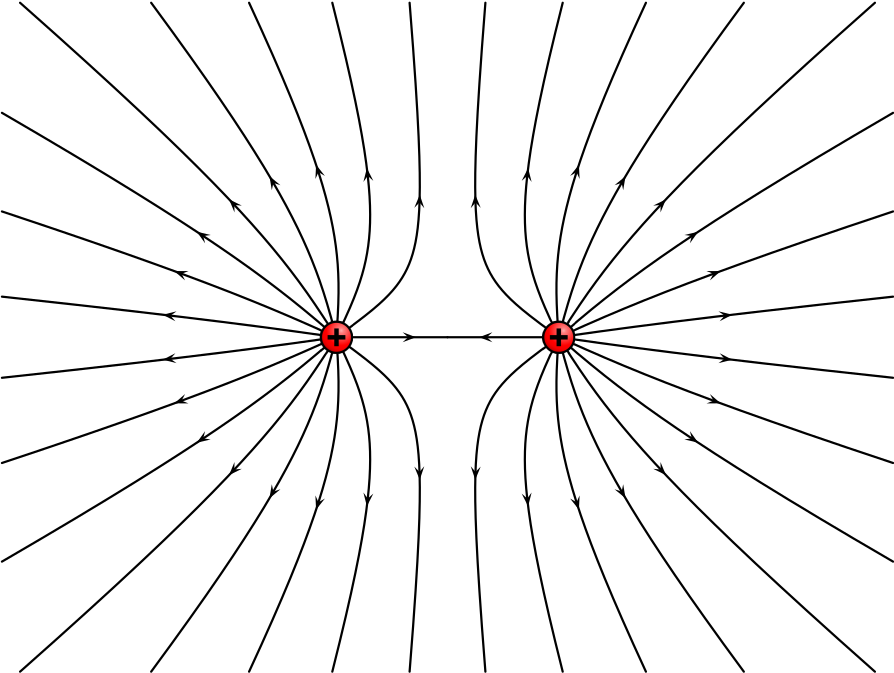
\includegraphics[height=4cm]{fig/fig-E-01.pdf}\hfill 
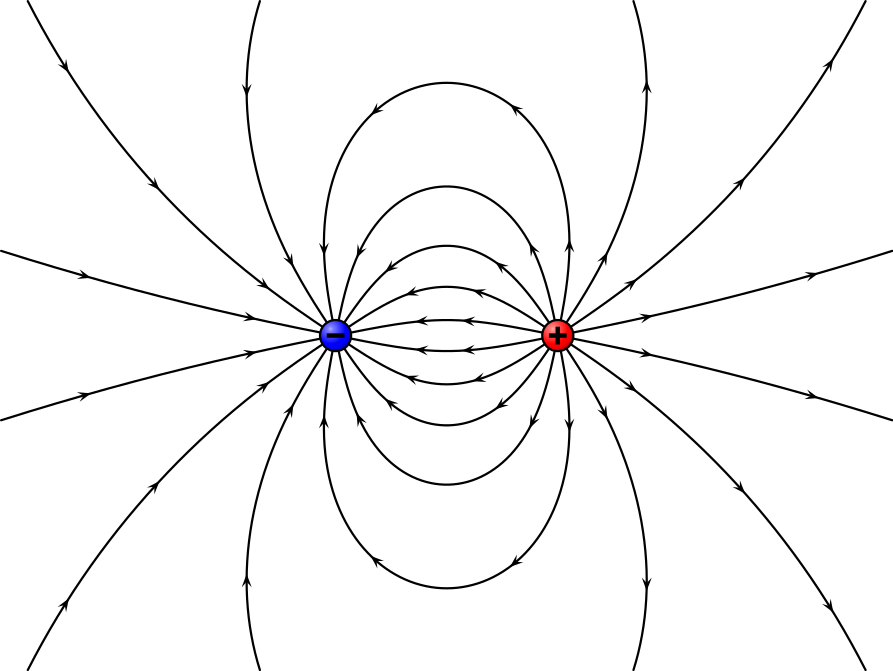
\includegraphics[height=4cm]{fig/fig-E-02.pdf}\hfill
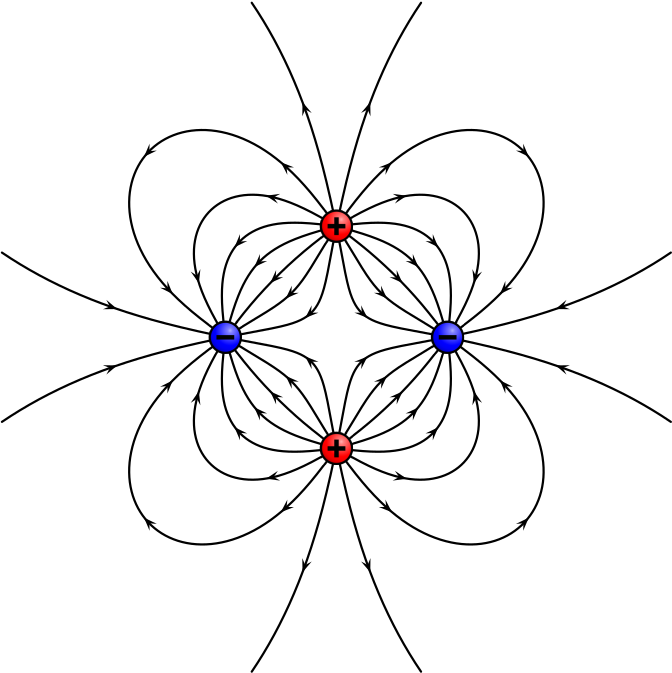
\includegraphics[height=4cm]{fig/fig-E-03.pdf}}
\caption{Ejemplos simples de líneas de campo eléctrico.}
\label{fig-E}
\end{figure}
\end{center}
\subsection{Potencial eléctrico}
Usando la identidad 
\begin{equation}
\frac{x_i-x_i'}{\left\vert \vec x-\vec x'\right\vert ^3}\equiv
-\partial_i\left( \frac{1}{\left\vert \vec x-\vec x'\right\vert
}\right), \label{id01}
\end{equation}
podemos escribir (\ref{cerho}) como
\begin{align}
E_i  & =\frac{1}{4\pi\varepsilon_0}\int_V\rho(x')\frac{\left(x_i-x_i'\right)
}{\left\vert \vec x-\vec x'\right\vert^3} dV' \\
&
=-\frac{1}{4\pi\varepsilon_0}\int_V\rho(x')\partial_i\left(\frac{1}{\left\vert
\vec x-\vec x'\right\vert }\right)  dV' \label{ein}\\
& =-\partial_i\left[\frac{1}{4\pi\varepsilon_0}\int_V\frac{\rho
(x')}{\left\vert \vec x-\vec x'\right\vert }dV'\right] \\
& =-\partial_i\phi ,
\end{align}
es decir,
\begin{equation}\marginnote{Campo a partir de potencial}
\boxed{\vec{E}(x)=-\vec\nabla\phi (x),} \label{E=nablaphi}
\end{equation}
donde hemos definido el \textbf{potencial eléctrico} $\phi(\vec x)$ por
\begin{equation}\marginnote{Potencial electrostático}
\boxed{\phi(\vec x):=\frac{1}{4\pi\varepsilon_0}\int_V\frac{\rho(\vec x')}{
\left\vert \vec x-\vec x'\right\vert }dV' +\text{constante}.}\label{perho}
\end{equation}

Note que es posible agregar una constante arbitraria a la definición del potencial. Por otro lado, es directo verificar que, como consecuencia directa de (\ref{E=nablaphi}), todo campo eléctrostático es irrotacional, es decir, su rotor es nulo:
\begin{equation}\marginnote{C. eléctrico irrotacional}
\boxed{\vec\nabla\times\vec{E}=\vec{0}.} \label{rotE0}
\end{equation}

Usando (\ref{E=nablaphi}), podemos expresar el potencial electrostático como una integral de línea del campo eléctrico:
\begin{equation}\marginnote{Potencial a partir de campo}
 \boxed{\phi(\vec{x})=\phi(\vec{x}_0)-\int_{\vec{x}_0}^{\vec{x}} \vec{E}\cdot
d\vec{x}.} \label{phiintE}
\end{equation}

Debido a (\ref{rotE0}) la integral (\ref{phiintE}) es independiente de la trayectoria que une los puntos $\vec{x}_0$ y $\vec{x}$, o equivalentemente,
\begin{equation}\marginnote{C. eléctrico sin circulación}
 \boxed{\oint_{\cal C}\vec{E}\cdot d\vec{x}=0,} \label{ointE0}
\end{equation}
para toda curva cerrada $\cal C$. Note además que de esta propiedad se desprende que las líneas de campo electrostático no pueden ser cerradas. En efecto, si existiese una línea de campo eléctrico cerrada ${\cal C}$, entonces podemos evaluar $\oint_{\cal C}\vec{E}\cdot d\vec{x}$ (la ``circulación del campo $\vec{E}$") sobre esta curva. Pero sobre una línea de campo se satisface (\ref{dlc}), de modo que
\begin{align}
\oint_{\cal C}\vec{E}\cdot d\vec{x} &= \oint_{\cal C}\frac{d\vec{x}}{d\lambda}\cdot d\vec{x} \\
&= \oint_{\cal C}\frac{d\vec{x}}{d\lambda}\cdot \frac{d\vec{x}}{d\lambda}\,d\lambda \\
&= \oint_{\cal C}\left|\frac{d\vec{x}}{d\lambda}\right|^2 d\lambda \\
&>0 ,
\end{align}
en contradicción con (\ref{ointE0}).

Note que como consecuencia de (\ref{E=nablaphi}) o, equivalentemente, de (\ref{phiintE}) el vector campo eléctrico es siempre \textit{normal a las superficies equipotenciales} (definidas como aquellos puntos que satisfacen $\phi(\vec{x})=\text{cte.}$) y su \textit{sentido es siempre hacia regiones de menor potencial}.

\section{Ley de Gauss}
Usando (\ref{ein}) podemos calcular la divergencia del campo eléctrico:
\begin{eqnarray}
\partial_iE_i &=&-\partial_i\left[
\frac{1}{4\pi\varepsilon_0}\int_V\rho(x')\partial_i\left(\frac{1}{\left\vert
\vec x-\vec x'\right\vert }\right)  dV'\right] \\
&=&-
\frac{1}{4\pi\varepsilon_0}\int_V\rho(x')\partial_i\partial_i\left(\frac{1}{
\left\vert \vec x-\vec x'\right\vert }\right)  dV' \\
&=&-
\frac{1}{4\pi\varepsilon_0}\int_V\rho(x')\nabla^2\left(\frac{1}{\left\vert
\vec x-\vec x'\right\vert }\right)  dV' \\
&=&-
\frac{1}{4\pi\varepsilon_0}\int_V\rho(x')\left[-4\pi\delta^{(3)}(x_i-x_i')\right]
dV' \\
&=& \frac{1}{\varepsilon_0}\int_V\rho(x')\delta^{(3)}(x_i-x_i')\, dV' \\
&=& \frac{1}{\varepsilon_0}\rho(x).
\end{eqnarray}
Obtenemos así la \textbf{forma diferencial de la ley de Gauss}\footnote{Carl Friedrich Gauss, (1777-1855): matemático, astrónomo y físico alemán, ver \url{http://es.wikipedia.org/wiki/Carl_Friedrich_Gauss}.}:
\begin{equation}\marginnote{Ley de Gauss diferencial}
\boxed{\partial_iE_i =\frac{1}{\varepsilon_0}\rho(x).} \label{leygauss-dif}
\end{equation}
Usando el teorema de la divergencia (de Gauss!) para un volumen $V$ arbitrario
con borde $S=\partial V$, obtenemos
\begin{eqnarray}
\int_V\partial_iE_i\,dV  &=&\frac{1}{\varepsilon_0}\int_V\rho(x)dV ,\\
\oint_S E_idS_i &=&\frac{1}{\varepsilon_0}q_V,
\end{eqnarray}
donde $q_V$ es la carga neta en el volumen $V$. En notación vectorial:
\begin{equation}\marginnote{Ley de Gauss integral}
\boxed{\oint_S \vec{E}\cdot d\vec{S} =\frac{1}{\varepsilon_0}q_V .}
\end{equation}

Esta es la \textbf{forma integral de la ley de Gauss}. Es importante recordar que la ley de Gauss en su forma integral es válida \textit{para todo volumen} $V$ y su correspondiente superficie ``gaussiana"\, $\partial V$. Debido a esta propiedad, la forma integral de la ley de Gauss resulta particularmente eficiente para determinar campos eléctricos en situaciones altamente simétricas, donde es posible elegir el volumen de modo que $\vec{E}$ sea \textit{constante} sobre $\partial V$ (o al menos, sobre partes de $\partial V$).

\subsection{Ejemplo: Plano infinito de densidad de carga constante}
\begin{equation}
\vec{E}(x)=\left\{\begin{array}{rl}\frac{\sigma}{2\varepsilon_0}\hat{x},& x>0 \\
-\frac{\sigma}{2\varepsilon_0}\hat{x},& x<0 \end{array}\right. .
\end{equation}

\subsection{Ejemplo: Cascarón esférico}
Consideremos primero el caso en el que una carga total $Q$ está distribuida uniformemente ($\rho=\rho_{\rm i}=\text{ cte.}$) en el interior de un cascarón esférico, de radios interior $a$ y exterior $b$.
La densidad interior $\rho_{\rm i}$ es dada por
\begin{equation}
\rho_{\rm i} = \frac{3Q}{4\pi(b^3-a^3)},
\end{equation}
por lo que la densidad, como función dependiente de la posición (o, en este caso el radio), es de la forma
\begin{equation}
\rho(r)=\left\{\begin{array}{cl}
0, & r<a\\
\rho_{\rm i}, & a\le r\le b,\\
0, & r>b
\end{array}\right.
\end{equation}
\begin{figure}[!h]
\centerline{\includegraphics[height=6cm]{fig/fig-esfera-hueca-densidad.pdf}}
\caption{Densidad volumétrica como función del radio.}
\label{fig_ehd}
\end{figure}
El campo eléctrico puede calcularse fácilmente usando la ley de Gauss, obteniendo
\begin{equation}
E(r)=\frac{Q}{4\pi\varepsilon_0}\times\left\{\begin{array}{cl}
0, & r<a\\
\frac{(r^3-a^3)}{r^2(b^3-a^3)}, & a\le r\le b,\\
\frac{1}{r^2}, & r>b
\end{array}\right.
\end{equation}
\begin{figure}[!h]
\centerline{\includegraphics[height=6cm]{fig/fig-esfera-hueca-campo.pdf}}
\caption{Magnitud del campo eléctrico como función del radio.}
\label{fig_ehc}
\end{figure}

El potencial, luego de imponer las condiciones de continuidad en $r=a$ y $r=b$ y elegir $\phi(r\to\infty)=0$ es dado por
\begin{equation}
\phi(r)=\frac{Q}{4\pi\varepsilon_0}\times\left\{\begin{array}{cl}
\frac{3(b^2-a^2)}{2(b^3-a^3)}, & r<a\\
-\frac{(2a^3+r^3)}{2r(b^3-a^3)}+\frac{3b^2}{2(b^3-a^3)}, & a\le r\le b,\\
\frac{1}{r}, & r>b
\end{array}\right.
\end{equation}
\begin{figure}[!h]
\centerline{\includegraphics[height=6cm]{fig/fig-esfera-hueca-potencial.pdf}}
\caption{Potencial eléctrico como función del radio.}
\label{fig_ehp}
\end{figure}

Estos gráficos fueron creados con el código contenido en \href{https://github.com/gfrubi/electrodinamica/blob/master/notebooks/esfera-cargada.ipynb}{este notebook}, en el que además puede variar los valores de $a$ y $b$.

\subsection{Ecuación de Poisson y Laplace}
Usando (\ref{E=nablaphi}) y (\ref{leygauss-dif}) obtenemos
\begin{equation}
\partial_iE_i  =-\partial_i\partial_i\phi=\frac{\rho}{\varepsilon_0},
\end{equation}
es decir, el potencial eléctrico satisface la \textbf{ecuación de
Poisson}\footnote{Siméon Denis Poisson (1781-1840): matemático francés, ver \url{http://es.wikipedia.org/wiki/Sim\%C3\%A9on_Denis_Poisson}.}:
\begin{equation}\marginnote{Ec. de Poisson}
\boxed{\nabla^2\phi=-\frac{\rho}{\varepsilon_0}.}\label{poisson}
\end{equation}

Como consecuencia, el potencial electrostático en una región libre de cargas
satisface la \textbf{ecuación de Laplace}\footnote{Pierre Simon Laplace (1749-1827): matemático, físico y astrónomo francés, \url{http://es.wikipedia.org/wiki/Laplace} .}:
\begin{equation}\marginnote{Ec. de Laplace}
\boxed{\nabla^2\phi=0.}\label{ecLap}
\end{equation}



\section{Condiciones de frontera para el campo eléctrico en una
interfase}\label{secCBE}

La figura \ref{DSCE1} muestra la interfase entre dos regiones separadas por una
superficie $S$ que posee una densidad superficial de carga $\sigma(x)$.
\begin{figure}[!h]
\centerline{\includegraphics[height=6cm]{fig/fig-superficie-frontera.pdf}}
\caption{Condiciones de frontera para el campo eléctrico.}
\label{DSCE1}
\end{figure}
Para estudiar las condiciones que el campo eléctrico satisface en esta
interfase, aplicamos primero la ley de Gauss, a la superficie gaussiana de la
figura \ref{DSCE2}:
\begin{figure}[!h]
\centerline{\includegraphics[height=5cm]{fig/fig-condicion-borde-electrico-01.pdf}}
\caption{Condición de frontera para la componente normal del campo eléctrico.}
\label{DSCE2}
\end{figure}
\begin{eqnarray}
\oint_{S} \vec{E}\cdot d\vec{S}&=&\int_{S_1}
\vec{E}_1\cdot d\vec{S}+\int_{S_2} \vec{E}_2 \cdot d\vec{S}+\int_{S_3}
\vec{E}\cdot d\vec{S}\\
&=& -(\vec{E}_1\cdot\hat{n})\Delta S+(\vec{E}_2\cdot\hat{n})\Delta S+0\\
&=& \frac{\sigma S}{\varepsilon_0},
\end{eqnarray}
donde $\Delta S$ es una superficie, cuyo \textit{vector unitario $\hat{n}$ está dirigido
desde la cara $1$ hacia la cara $2$}, que contiene una densidad de carga
$\sigma(\vec{x})$ $\left[ C/m^2\right]  $, y los campos eléctricos a
cada lado de la superficie son como se indica en la figura.

Por tanto, obtenemos
\begin{equation}\marginnote{Discontinuidad comp. normal}
\boxed{\vec{E}_2\cdot\hat{n}-\vec{E}_1\cdot\hat{n}=\frac{\sigma}
{\varepsilon_0}.}\label{saltoEn}
\end{equation}

Por otro lado, aplicando (\ref{ointE0}) a la curva de la figura \ref{DSCE3} obtenemos:
\begin{figure}[!h]
\centerline{\includegraphics[height=5cm]{fig/fig-condicion-borde-electrico-02.pdf}}
\caption{Condición de frontera para la componente tangencial del campo eléctrico.}
\label{DSCE3}
\end{figure}
\begin{eqnarray}
 \oint_{\cal C} \vec{E}\cdot d\vec{x}&=&\int_{{\cal C}_1} \vec{E}\cdot
d\vec{x}+\int_{{\cal C}_2} \vec{E}\cdot d\vec{x}+\int_{{\cal C}_3}
\vec{E}\cdot d\vec{x}+\int_{{\cal C}_4} \vec{E}\cdot d\vec{x} \\
&=& -(\vec{E}_1\cdot\hat{t})\ell +(\vec{E}_2\cdot\hat{t})\ell +0+0 \\
&=& 0.
\end{eqnarray}
De aquí encontramos que
\begin{equation}\marginnote{Continuidad comp. tangencial}
 \boxed{\vec{E}_2\cdot\hat{t}=\vec{E}_1\cdot\hat{t}.} \label{Etconst}
\end{equation}
Ya que la dirección del vector $\hat{t}$ es arbitraria (pero siempre
tangencial a la superficie $S$), la condición (\ref{Etconst}) implica que
 \textit{las componentes tangenciales (2 componentes linealmente idependientes) del campo eléctrico permanecen inalteradas
al cruzar la superficie} $S$.

\subsection{Conductores}

Los \textbf{conductores} son materiales que, aunque estén
eléctricamente neutros a nivel macros\-có\-pi\-co, poseen
una enorme cantidad de electrones ``libres'' (es decir,  no ligados a
los átomos, y que pueden moverse a través del conductor tan pronto como
exista un campo eléctrico que induzca su movimiento)
aptos para conducir la electricidad. La carga de estos electrones es
neutralizada (a escala macroscópica) por la de los protones que están en los n\'{u}cleos, que pueden considerarse fijos. Como ejemplo de conductores podemos mencionar a los metales y a los electrolitos (cambién conocidos como \textbf{soluciones iónicas}).

Si un conductor es cargado, o está en presencia de cargas externas, los electrones rápidamente\footnote{Como veremos más adelante el \textit{tiempo de relajación} es del orden de $\tau=\varepsilon/\sigma$ donde $\varepsilon$ es la \textit{constante dieléctrica} del material y $\sigma$ su \textit{conductividad}. Por ejemplo, para el cobre $\tau\approx 10^{-19}$s.} se desplazan hasta una situación de \textit{equilibrio}, es decir, un \textit{estado estacionario}. En este
estado el campo eléctrico (macroscópico) en el interior del conductor debe anularse ya que de otro modo la fuerza sobre ellos sería no nula, induciendo
movimiento. Por tanto, en situación estacionaria $\vec{E}=\vec{0}$ en el
\textit{interior} de los conductores. Como consecuencia de la ley de Gauss, la
densidad de carga en el interior del conductor se anula cuando éste
alcanza su estado estacionario. En otras palabras, \textit{un conductor en estado estacionario distribuye su carga neta sobre su superficie}.

Aplicando las condiciones de borde (\ref{saltoEn}) y (\ref{Etconst}) a la
interfase del conductor, y tomando en cuenta que en este caso
$\vec{E}_1=\vec{0}$, encontramos que \textit{en cada punto de la superficie (exterior) del conductor}
\begin{equation}\marginnote{Campo fuera de conductor}
 \vec{E}_2(x)=\frac{\sigma(x)}{\varepsilon_0}\hat{n}(x), \label{Econd}
\end{equation}
es decir, que el campo eléctrico es normal a la superficie, y proporcional a la densidad de carga en cada punto de ésta. El potencial eléctrico, por otro lado, es necesariamente constante tanto dentro del conductor como sobre su superficie.

\subsection{Sobre (dis)continuidad de los campos}
 Idealmente, al menos clásica y macroscópicamente, la distribución de carga descrita por la densidad volumétrica $\rho(\vec{x})$ debiese ser una función \textit{finita y continua} en todo punto. Como consecuencia, el campo eléctrico y el potencial serían, de acuerdo a (\ref{cerho}) y (\ref{perho}), también funciones finitas y contínuas. Sin embargo, comúnmente es \textit{conveniente} idealizar la distribución de cargas, considerando que ésta está limitada a una superficie bidimensional (es decir, de sección transversal despreciable). Este caso corresponde a considerar una densidad volumétrica $\rho$ singular (discontinua y divergente)\footnote{Por ejemplo, la densidad volumétrica correspondiente a una carga distribuida en todo el plano $xy$, con densidad superficial de carga $\sigma(x,y)$ puede escribirse como $\rho(x,y,z)=\sigma(x,y)\delta(z)$.}. En este caso, el campo eléctrico poseerá, en general, \textit{discontinuidades} en la superficie donde $\rho$ es singular, tal como analizamos en la sección \ref{secCBE}, pero será \textit{finito en todo punto}. El potencial, por otro lado, será una \textit{función continua y diferenciable por tramos}. En resumen, para distribuciones de carga singulares que incluyan distribuciones superficiales de carga, el potencial puede siempre considerarse como una función continua, el campo eléctrico (proporcional a las derivadas del potencial) puede tener discontinuidades, mientras que las segundas derivadas del potencial (proporcionales a las primeras derivadas del campo eléctrico y, a través de la ecuación de Poisson (\ref{poisson}), ligadas a la densidad volumétrica de carga) pueden poseer regiones (superficies) singulares. En el caso de que la distribución de carga se modele incluyendo cargas puntuales o líneas de carga, el potencial ya no será finito en todo punto.


\section{Solución de la ecuación de Laplace}
\subsection{Coordenadas Esféricas}
Una solución general (finita sobre el eje $z$) de la ecuación de Laplace en coordenadas esféricas puede escribirse como:
\begin{equation}
  \boxed{\phi(r,\theta,\varphi) = \sum_{l=0}^\infty\sum_{m=-l}^l\left[
  A_{lm}  r^l + B_{lm}  r^{-(l+1)}\right]  Y_{lm}(\theta,\varphi),}
  \label{est31b}
\end{equation}
donde $A_{lm}$ y $B_{lm}$ son coeficientes constantes. Note que estos
coeficientes son en general complejos.

Si, como caso particular, el potencial tiene simetría axial, es decir no
depende de la coordenada $\varphi$, entonces la expansión se reduce a
\begin{eqnarray}
  \phi(r,\theta) &=& \sum_{l=0}^\infty\left[
  A_{l0}  r^l + B_{l0}  r^{-(l+1)}\right]  Y_{l0}(\theta,\varphi) \\
&=&\sum_{l=0}^\infty\left[  A_{l0}  r^l + B_{l0}
r^{-(l+1)}\right]\sqrt{\frac{2l+1}{4\pi}}\,P_l(\cos\theta) ,
\end{eqnarray}
o, equivalentemente,
\begin{equation}\label{phiaxial}
\boxed{\phi(r,\theta)=\sum_{l=0}^\infty\left[  a_l\,  r^l +
\frac{b_l}{r^{l+1}}\right]\,P_l(\cos\theta),}
\end{equation}
donde $a_l$ y $b_l$ son nuevos coeficientes reales constantes.

\subsubsection{Ejemplo: Esfera conductora en un campo eléctrico externo homogéneo}\label{sec:esfcond}

Consideramos una esfera conductora de radio $R$ ubicada en un campo externo inicial homogéneo $\vec{E}_0$. Elegimos los ejes coordenados de modo que el origen coincida con el centro de la esfera y el eje $z$ con la dirección del campo externo, es decir, $\vec{E}_0=E_0\hat{z}$.

Luego de ubicar la esfera en el campo externo, las cargas libres en ella se reacomodan rápidamente. En la situación estacionaria final el campo eléctrico en el interior de la esfera es nulo, es decir, $\vec{E}=0$ para $r<R$. Como consecuencia directa $\phi=\text{cte.}$ para $r<R$. Podemos elegir esta constante igual a cero, de modo que
\begin{equation}
\phi(r,\theta)\stackrel{!}{=}0, \qquad r<R.
\end{equation}

Por otro lado, de acuerdo a (\ref{Econd}) el campo eléctrico en la superficie externa del conductor es radial, y proporcional a la densidad de carga $\sigma$. Debido que el sistema es simétrico bajo rotaciones en torno a la dirección de $\vec{E}$, tendremos que $\phi=\phi(r,\theta)$ y $\sigma=\sigma(\theta)$. Finalmente, fuera de la esfera el potencial satisface la ec. de Laplace, por lo que éste debe tener la forma general (\ref{phiaxial}). Por lo tanto, para determinar el potencial en todo punto basta determinar los coeficientes (constantes) $a_l$ y $b_l$.

Una condición necesaria es que asimptóticamente, es decir, para $r\to\infty$, el campo debe tender al campo externo inicial ya que los efectos de las cargas inducidas en la esfera serán cada vez menores en puntos cada vez más alejados, es decir, $\vec{E}\to\vec{E}_0 $. Esta condición es equivalente a 
\begin{equation}
\phi\to -E_0z+\alpha=-E_0r\cos\theta+\alpha,
\end{equation}
donde $\alpha$ es una constante a determinar. Aplicando esta condición a la expansión (\ref{phiaxial}) encontramos que necesariamente
\begin{equation}
a_0=\alpha, \qquad a_1=-E_0, \qquad a_2=a_3=\cdots =0,
\end{equation}
por lo que el potencial en todo punto  fuera de la esfera se reduce a 
\begin{equation}
\phi(r,\theta)=\alpha -E_0 r\cos\theta +
\sum_{l=0}^\infty\frac{b_l}{r^{l+1}}P_l(\cos\theta), \qquad r\ge R.
\end{equation}

Como el potencial es una función contínua, debemos tener que
\begin{equation}
\phi(R,\theta)=\alpha -E_0 R\cos\theta +
\sum_{l=0}^\infty\frac{b_l}{R^{l+1}}P_l(\cos\theta)=0, \qquad \forall \theta.
\end{equation}

De aquí, y ya que los polinomios de Legendre son funciones linealmente independientes, encontramos que necesariamente
\begin{equation}
\alpha+\frac{b_0}{R}=0, \qquad -E_0R+\frac{b_1}{R^2}=0, \qquad b_2=b_3=\cdots =0.
\end{equation}

Con esto, el potencial se reduce a
\begin{equation}\label{phialpha}
\phi(r,\theta)=\alpha -E_0 r\cos\theta -\alpha\frac{R}{r}+E_0 \frac{R^3}{r^2}\cos\theta. 
\end{equation}

Finalmente, debemos determinar la constante $\alpha$, que es proporcional a la carga neta de la esfera. En efecto, usando (\ref{Econd}) podemos calcular la densidad superficial de carga en la esfera:
\begin{align}
\sigma(\theta) &= \varepsilon_0\, \vec{E}(R,\theta)\cdot\hat{r} \\
&= -\varepsilon_0 \frac{\partial\phi}{\partial r}(R,\theta) \\
&= -\varepsilon_0\left[-E_0\cos\theta+\frac{\alpha}{R}-2E_0\cos\theta\right]\\
&= \varepsilon_0\left[3E_0\cos\theta-\frac{\alpha}{R}\right].
\end{align}

La carga neta de la esfera es entonces
\begin{align}
Q &= \oint_S\sigma(\theta)\,dS \\
&= 2\pi R^2 \int_0^\pi \sigma(\theta)\sin\theta\,d\theta \\
&= 2\pi \varepsilon_0R^2 \int_0^\pi \left[3E_0\cos\theta-\frac{\alpha}{R}\right] \sin\theta\,d\theta \\
&= 2\pi \varepsilon_0R^2 \left[ 0-\frac{2\alpha}{R}\right] \\
&= -4\pi \varepsilon_0R \alpha .
\end{align}

En otras palabras, 
\begin{equation}
\alpha=-\frac{Q}{4\pi \varepsilon_0}\frac{1}{R}.
\end{equation}
Con este resultado, el potencial (\ref{phialpha}) puede escribirse como 
\begin{equation}
\phi(r,\theta)=-\frac{Q}{4\pi\varepsilon_0 R}+\frac{Q}{4\pi\varepsilon_0}\frac{1}{r} -E_0 \left(1-\frac{R^3}{r^3}\right)r\cos\theta.
\end{equation}

Como vemos, los primeros dos términos son independientes del campo externo y representan el potencial de la carga neta de la esfera (que hemos supuesto aislada). El tercer término es el campo externo inicial y por lo tanto el último término describe el campo eléctrico inducido producto de la polarización de la esfera conductora.
\begin{figure}[!h]
\centerline{\includegraphics[height=5.5cm]{fig/fig-esfera-conductora-campo-externo.pdf}
\hspace{1cm}
\includegraphics[height=5.5cm]{fig/fig-esfera-conductora-campo-externo-2.pdf}}
\caption{Campo eléctrico de una esfera conductora neutra en un campo eléctrico externo. El gráfico de la izquierda (normalizado) fue creado usando \href{https://github.com/gfrubi/electrodinamica/blob/master/figuras-editables/fig-esfera-conductora-campo-externo-raw.py}{este script} Python. La figura de la derecha fue generada usando \href{http://commons.wikimedia.org/wiki/User:Geek3/VectorFieldPlot}{VectorFieldPlot}, a partir de \href{http://commons.wikimedia.org/wiki/File:VFPt_superconductor_ball_E-field.svg}{este} archivo original.}
\label{fig:ecce}
\end{figure}

El campo eléctrico es entonces dado por
\begin{equation}
\vec{E}(r,\theta) = E_r\hat{r}+E_\theta\hat{\theta},
\end{equation}
con 
\begin{equation}
E_r = -\frac{\partial\phi}{\partial r} = \frac{Q}{4\pi\varepsilon_0}\frac{1}{r^2}+E_0 \left(1+2\frac{R^3}{r^3}\right)\cos\theta, \quad E_\theta = -\frac{1}{r}\frac{\partial\phi}{\partial\theta} =-E_0 \left(1-\frac{R^3}{r^3}\right)\sin\theta .
\end{equation}
En la figura \ref{fig:ecce} se muestra la forma de este campo, en el caso en que $Q=0$.


%\subsection{Coordenadas Cilíndricas}

%\subsection{Coordenadas Cartesianas}

 \section{Solución de la ecuación de Poisson} 
 \subsection{Solución en términos de Funciones de Green*}\label{Green}
 La ecuación de Poisson \eqref{poisson} para el potencial es una \textit{EDP lineal elíptica inhomogénea}. Una forma de encontrar soluciones de este tipo de ecuaciones es usando el método de las \textbf{funciones de Green}. En nuestro caso, se dice que $G(\vec{x},\vec{x}')$ es una función de Green del operador Laplaciano si satisface
\begin{equation}\label{EDPG}
\nabla^2G(\vec{x}',\vec{x})=\delta^{(3)}(\vec{x}-\vec{x}').
\end{equation} 

Si se conoce una función de Green entonces la solución de la ecuación de Poisson para el potencial en una región $V$ puede expresarse de la forma siguiente:
\begin{align}
\phi(\vec{x}) &= -\frac{1}{\varepsilon_0}\int_VG(\vec{x},\vec{x}')\rho(\vec{x}')dV'+\oint_{\partial V}\left[\phi(\vec{x}')\vec\nabla' G(\vec{x},\vec{x}')-G(\vec{x},\vec{x}')\vec\nabla'\phi(\vec{x}')\right]\cdot d\vec{S}' \\
&=  -\frac{1}{\varepsilon_0}\int_VG(\vec{x},\vec{x}') \rho(\vec{x}')dV'+\oint_{\partial V}\left[\phi(\vec{x}')\frac{\partial G}{\partial n'}(\vec{x},\vec{x}')-G(\vec{x},\vec{x}')\frac{\partial\phi}{\partial n'}(\vec{x}')\right]dS'
\end{align}

Introduciendo el campo eléctrico en el segundo término del lado derecho podemos escribir
\begin{equation}\label{solPoisson}
\phi(\vec{x})= -\frac{1}{\varepsilon_0}\int_VG(\vec{x},\vec{x}') \rho(\vec{x}')dV'+\oint_{\partial V}\left[\phi(\vec{x}')\frac{\partial G}{\partial n'}(\vec{x},\vec{x}')+G(\vec{x},\vec{x}')E_n(\vec{x}')\right]dS',
\end{equation}
donde $E_n:=\vec{E}\cdot\hat{n}$ es la componente del campo eléctrico normal a la superficie $\partial V$ (con $\hat{n}$ orientado hacia el exterior del volumen $V$).

Por otro lado, la función de Green no es única. Si $G_1(\vec{x},\vec{x}')$ es una función de Green entonces $G_2(\vec{x},\vec{x}')=G_1(\vec{x},\vec{x}')+H(\vec{x},\vec{x}')$ también lo será si $H$ es una solución del problema homogéneo: en nuestro caso de la ecuación de Laplace, $\nabla^2H(\vec{x},\vec{x}')=0$. Esta arbitrariedad en la definición de la función de Green es de hecho una ventaja, puesto que en general no se tiene información \textit{simultánea} del potencial y la componente normal del campo en la frontera $\partial V$. Por esto, es conveniente elegir una función de Green de modo que los términos del lado derecho de \eqref{solPoisson} puedan efectivamente ser evaluados. Por ejemplo, si se conoce el potencial\footnote{condición de borde tipo Dirichlet.} en $\partial V$ (típicamente, en situaciones donde $\partial V$ coincide con la superfice de conductores conectados a baterías suministrando una diferencia de potencial conocida) entonces es conveniente usar una \textit{función de Green que se anule en la frontera}, $G(\vec{x},\vec{x}')=0$, $\forall$ $\vec{x}'\in\partial V$. En este caso, la solución se reduce a
\begin{equation}\label{solPoissonDirichlet}
\phi(\vec{x})= -\frac{1}{\varepsilon_0}\int_VG(\vec{x},\vec{x}') \rho(\vec{x}')dV'+\oint_{\partial V}\phi(\vec{x}')\frac{\partial G}{\partial n'}(\vec{x},\vec{x}')dS',
\end{equation}

 Por otro lado, si se conoce la componente normal del campo en la frontera\footnote{condición de borde tipo Neumann.} (por ejemplo, en situaciones donde se dispone de información sobre la densidad de carga superficial en $\partial V$) entonces parece conveniente usar una función de Green tal que su derivada normal sobre la frontera sea nula. Lamentablemente, esta condición \textit{no es posible de implementar} ya que necesariamente\footnote{Use el teorema de Gauss sobre la integral de volumen de \eqref{EDPG} para verificar esto!.} debe cumplirse que
\begin{equation}\label{intGn}
\oint_{\partial V}\frac{\partial G}{\partial n'}dS'=1.
\end{equation}

Una condición un poco menos restrictiva, y factible de implementar consistentemente, es imponer que la derivada normal de la función de Green sea \textit{constante en la frontera}. Entonces, \eqref{intGn} requiere que
\begin{equation}
\frac{\partial G}{\partial n'}(\vec{x},\vec{x}')=\frac{1}{S}, \qquad \vec{x}'\in\partial V,
\end{equation}
donde $S$ es el área total de la frontera, $S:=\oint_{\partial V} dS$. En este caso, la solución para el potencial adopta la forma
\begin{equation}
\phi(\vec{x})= \left\langle\phi\right\rangle_S-\frac{1}{\varepsilon_0}\int_VG(\vec{x},\vec{x}') \rho(\vec{x}')dV'+\oint_{\partial V}G(\vec{x},\vec{x}')E_n(\vec{x}')dS',
\end{equation}
donde
\begin{equation}
\left\langle\phi\right\rangle_S:=\frac{1}{S}\oint_{\partial V}\phi(\vec{x}')\,dS'
\end{equation}
es el \textit{valor promedio del potencial sobre} $\partial V$.

Finalmente, la función de Green más conocida del operador Laplaciano es dada por
\begin{equation}
G(\vec{x}-\vec{x}')=-\frac{1}{4\pi}\frac{1}{|\vec{x}-\vec{x}'|}.
\end{equation}
Esta función de Green particular posee las propiedades adicionales de ser \textit{simétrica bajo rotaciones respecto al punto $\vec{x}'$}, \textit{depender sólo de la diferencia $\vec{x}-\vec{x}'$} y de \textit{anularse en el infinito} (para todo valor finito de $\vec{x}'$). Debido a estas propiedades esta función de Green está directamente relacionada con la solución de la ecuación de Poisson en el caso en que la región $V$ cubre todo el espacio y se asume que el campo eléctrico se anula en el infinito\footnote{más rápido que $1/r$, es decir, tal que $\lim_{|x|\to\infty}|\vec{E}|r=0$.}, de modo que el potencial se reduce a
\begin{equation}
\phi(\vec{x})= \left\langle\phi\right\rangle_\infty+\frac{1}{4\pi\varepsilon_0}\int_V\frac{\rho(\vec{x}')}{|\vec{x}-\vec{x}'|}dV'.
\end{equation}

\subsection{Unicidad de la solución}\label{sec:uniP}
A continuación probaremos que \textit{la solución de la ecuación de Poisson es única} (salvo una constante aditiva), en una región $V$, para valores dados del potencial \textit{o de la componente normal del campo} en la frontera\footnote{Condiciones de borde tipo Dirichlet o tipo Neumann, respectivamente.} $\partial V$. Para esto, suponemos que existen dos soluciones distintas de \eqref{poisson} en $V$, $\phi_1(\vec{x})$ y $\phi_1(\vec{x})$, que \textit{satisfacen las mismas condiciones de borde}, es decir, su valor es conocido en $\partial V$, o bien su derivada normal es conocida en esta frontera.

Definimos la diferencia $U(\vec{x}):=\phi_1(\vec{x})-\phi_2(\vec{x})$ que será entonces una solución de la ecuación de Laplace, $\nabla^2U=0$. En la frontera $\partial V$ esta función satisface $U=0$ o bien ${\partial U}/{\partial n}=0$, ya que asumimos que $\phi_1$ y $\phi_2$ satisfacen las mismas condiciones de borde (tipo Dirichlet, o bien tipo Neumann). Usamos ahora la identidad\footnote{Esta identidad es un caso particular de la así llamada \textit{primera identidad de Green}.}
\begin{equation}
 \int_V\left[\left|\vec\nabla U\right|^2+U\nabla^2U\right]  \,dV
 \equiv\oint_SU\frac{\partial U}{\partial n}\,dS,
 \end{equation}
que puede ser verificada fácilmente usando el teorema de Gauss. En nuestro caso, dada la EDP y las condiciones de borde que $U$ satisface, la identidad implica que
\begin{equation}
 \int_V\left|\vec\nabla U\right|^2dV=0.
\end{equation}

Como consecuencia, la función $U$ debe ser \textit{constante}\footnote{En principio, esto sería válido excepto (a lo sumo) en un conjunto de medida cero. Sin embargo, esta posibilidad queda descartada si el potencial es una función continua.}, por lo que las dos soluciones $\phi_1$ y $\phi_2$ sólo pueden diferir por una constante, representando la misma solución física\footnote{Más aún, para condiciones de borde tipo Dirichlet, esta constante es necesariamente nula.}.

Es importante notar que este resultado implica que, en general, es inconsistente intentar encontrar una solución de la ecuación de Poisson \textit{imponiendo simultáneamente el valor del potencial y de su derivada normal en la frontera}.

Note que los teoremas anteriores implican que el campo eléctrostático en una región $V$ queda totalmente determinado por la densidad de carga en el interior del volumen $V$, y por las condiciones de borde en la frontera $\partial V$. Una de las múltiples consecuencias de este hecho es que el campo al interior de un volumen de forma arbitraria, cuya frontera es mantenida a un potencial fijo (por ejemplo, por medio de un conductor puesto ``a tierra'') es \textit{independiente de la distribución de cargas en el exterior}. De esta forma, es posible aislar una región de las influencias eléctricas externas (``\href{https://es.wikipedia.org/wiki/Jaula_de_Faraday}{jaula de Faraday}'').


\section{Método de las imágenes}
Como vimos la sección \ref{sec:uniP}, la solución de la ecuación de Poisson, que determina el potencial electrostático y por lo tanto también el campo eléctrico, es única dadas las condiciones de borde apropiadas. Debido a esto, si
obtenemos, \textit{por cualquier método}, una solución que respete las condiciones de
borde dadas, ésta es \textit{la} solución del problema en ese volumen. El \textit{método de
las imágenes} suministra un procedimiento para encontrar una solución en
casos donde el sistema contiene conductores (perfectos) a potencial constante
(típicamente, ``puestos a tierra'') y la geometría de los conductores y las
cargas es simple. Para ello, se introducen \textit{cargas ficticias} en
posiciones apropiadas \textit{fuera de nuestro volumen $V$ de interés} tales que el campo creado por el sistema de cargas reales
+ ficticias satisface las condiciones de borde.

En otras palabras, el método de las imágenes se basa en el hecho que la
solución para el campo eléctrico en una región finita $V$ con una
distribución de carga conocida y potenciales dados en su superficie
$\partial V$ pueden ser los mismos (\underline{en $V$}) que los campos generados por la
misma distribución de carga en $V$ \textit{y por otra distribución de carga
diferente fuera de $V$}. Por esto, para solucionar el problema ``real'', en el
que la distribución de carga en $V$ y los potenciales en $\partial V$ son conocidos, se
puede considerar el problema ``ficticio'' de encontrar las cargas ``imagenes''
fuera de $V$ tales que la distribución de cargas total (reales e imágenes)
satisfaga las condiciones de contorno en $\partial V$. Los campos así encontrados son
solución del problema original, dentro (pero \underline{no} fuera) de $V$. Como veremos, el método de las imágenes básicamente provee un método heurístico para encontrar la función de Green apropiada a las condiciones de borde de un cierto problema físico.



\subsection{Conductor plano y carga puntual}
\begin{figure}[!h]
\centerline{\includegraphics[height=6cm]{fig/fig-carga-imagen-01.pdf}}
\caption{Conductor plano, carga real $q$ e imagen $q'$.}
\label{ci01}
\end{figure}
Consideremos la situación donde una carga puntual $q$ se encuentra a una distancia $d$ de un plano conductor (infinito) ``puesto a tierra'' (de modo que su potencial es igual al potencial en el infinito, elegido como $\phi_\infty=0$). Eligiendo los ejes coordenados como lo indica la figura \ref{ci01}, tendremos que en la situación estacionaria $\phi(x)=0$ para $x\le 0$. 

El potencial no es simplemente el de la carga puntual $\phi_{\rm puntual} = {q}/{4\pi\epsilon_0 r}$, puesto que la presencia de la carga $q$ induce una cierta distribución de carga en la superficie del conductor. Luego, el potencial total es debido en parte a $q$ y en otra parte a la distribución de carga inducida. Pero, ¿cómo calculamos el potencial si no conocemos cuánta carga es inducida y cómo esta se distribuye? 

Desde un punto de vista matemático, nuestro problema es resolver la ecuación de Poisson en la región $x>0$, con una carga puntual $q$ situada en $\vec{x}_q=d\hat{x}$ sujeta a las condiciones de contorno: a) $\phi = 0 $ en $x=0$ (pues el conductor está puesto a tierra), y b) $\phi\rightarrow 0$ lejos de la carga (cuando $x^2 + y^2 + z^2 \gg d^2$). Usando el método de las imágenes resolvemos el problema equivalente obtenido al reemplazar el plano conductor por una carga ficticia (imagen) $q'$ ubicada en la posición $x=-d'<0$. El potencial de la configuración de carga real más carga imagen es entonces
\begin{equation}
 \phi(x)=\frac{1}{4\pi\varepsilon_0}\left[\frac{q}{\sqrt{(x-d)^2+y^2+z^2}}+\frac
{q'}{\sqrt{(x+d')^2+y^2+z^2}}\right].
\end{equation}
La condición que $\phi=0$ sobre el plano, es decir, para todo punto con $x=0$,
se satisface sólo si
\begin{equation}
 d'=d, \qquad q'=-q.
\end{equation}
Por lo tanto, la solución para el potencial en todo punto con $x\ge 0$ es dada por
\begin{equation}\label{phicpplano}
 \phi(x)=\frac{q}{4\pi\varepsilon_0}\left[\frac{1}{\sqrt{(x-d)^2+y^2+z^2}}-\frac
{1}{\sqrt{(x+d)^2+y^2+z^2}}\right], \qquad x\ge 0.
\end{equation}
Note que esta solución define un potencial no nulo para la región $x < 0$. Sin embargo, esto no afecta la solución del problema original, pues nuestra región de interés es la región $x \ge 0$.
\begin{center}
\begin{figure}[H]
\centerline{\includegraphics[height=4.5cm]{fig/fig-metodo-imagen-plano-01.pdf}
\hspace{2cm}
\includegraphics[height=4.5cm]{fig/fig-metodo-imagen-plano-02.pdf}}
\caption{Campo eléctrico de plano conductor (puesto a Tierra) y carga puntual. 
Figuras adaptadas de  \href{http://commons.wikimedia.org/wiki/File:VFPt_image_charge_plane_horizontal.svg}{este} y \href{http://commons.wikimedia.org/wiki/File:VFPt_image_charge_plane.svg}{este} archivo original.}
\label{fig:pyc}
\end{figure}
\end{center}
La densidad de carga inducida en el conductor puede calcularse usando
\begin{equation}
 \sigma(y,z)=\varepsilon_0
\vec{E}\cdot\hat{n}=-\varepsilon_0\left.(\partial_x\phi)\right|_{x=0}
\end{equation}
que, luego de algo de álgebra, resulta ser
\begin{equation}
 \sigma(y,z)=-\frac{q}{2\pi}\frac{d}{(d^2+y^2+z^2)^{3/2}}.
\end{equation}
Con esto, podemos calcular la carga total inducida sobre el conductor,
\begin{equation}
Q_{\rm ind} = \int \sigma(y,z) dS.
\end{equation}
La integral resulta más simple de calcular en coordenadas polares, ya que
\begin{equation}
Q_{\rm ind} = \int_0^{2\pi} \int_0^\infty \dfrac{-qd}{2\pi (r^2 + d^2)^{3/2}} \ r  dr  d\varphi = \left. \dfrac{qd}{\sqrt{r^2 + d^2}} \right|_{0}^{\infty} = -q,
\end{equation}
lo que es consistente con nuestra elección inicial para el valor de la carga imagen $q'$.

Por otro lado, la fuerza que ejerce el plano sobre la carga puede ser calculada usando
\begin{equation}
\vec{F}_q=q\vec{E}',
\end{equation}
donde $\vec{E}'$ es el campo \textit{externo} que actúa sobre $q$, es decir, el campo
determinado por el potencial
\begin{equation}
 \phi'(x)=-\frac{q}{4\pi\varepsilon_0}\frac{1}{\sqrt{(x+d)^2+y^2+z^2}},
\qquad x>0,
\end{equation}
evaluado en la posición en que se ubica la carga $q$, es decir,
\begin{eqnarray}
 \vec{F}_q&=&-q(\vec{\nabla}\phi')|_{\vec{x}_q} \\
&=&-\frac{q^2}{16\pi\varepsilon_0d^2}\,\hat{x}.
\end{eqnarray}
Note que esta fuerza es la misma que ejerce(ría) la carga imagen sobre la carga real.

\subsubsection{Función de Green asociada}
En la sección anterior hemos situado el sistema coordenado de modo que la carga tenía posicion $d\hat{x}$. Podemos reescribir el resultado para una carga puntual ubicada en una posición arbitraria $\vec{x}'$ en $V$. Manteniendo el origen del sistema de coordenadas en algún punto del plano, podemos entonces escribir la posición \textit{de la carga imágen} como
\begin{equation}
\vec{x}'_{\rm i} = \vec{x}'-2(\vec{x}'\cdot\hat{n})\hat{n},
\end{equation}
donde $\hat{n}$ es el vector unitario perpendicular a la superficie del conductor. Con esto, potencial \eqref{phicpplano} puede ser escrito en la forma siguiente:
\begin{align}
\phi(\vec{x}) &= \frac{q}{4\pi\varepsilon_0}\left[\frac{1}{\left|\vec{x}-\vec{x}'\right|}-\frac{1}{\left|\vec{x}-\vec{x}'_{\rm i}\right|}\right] \\
&= \frac{q}{4\pi\varepsilon_0}\left[\frac{1}{\left|\vec{x}-\vec{x}'\right|}-\frac{1}{\left|\vec{x}-\vec{x}'+2(\vec{x}'\cdot\hat{n})\hat{n}\right|}\right]
\end{align}

Si ahora definimos
\begin{align}
G(\vec{x},\vec{x}') &:= -\frac{\varepsilon_0}{q}\phi(\vec{x}) \\
&= -\frac{1}{4\pi}\left[\frac{1}{\left|\vec{x}-\vec{x}'\right|}-\frac{1}{\left|\vec{x}-\vec{x}'+2(\vec{x}'\cdot\hat{n})\hat{n}\right|}\right], \label{Greenplano}
\end{align}
entonces esta función satisface todas las propiedades de una función de Green en el dominio $V$, con condiciones de borde tipo Dirichlet nulas en su frontera::
\begin{itemize}
\item $\nabla^2G(\vec{x},\vec{x}')=\delta^{(3)}(\vec{x}-\vec{x}')$, $\forall \vec{x}\in V$.
\item $G(\vec{x},\vec{x}')=0$, $\forall \vec{x}\in \partial V$.
\item $G(\vec{x},\vec{x}')=G(\vec{x}',\vec{x})$.
\end{itemize}

Como consecuencia, podemos usar esta función para encontrar una forma analítica para el potencial \textit{en una situación física más general}: el campo fuera de un conductor plano muy grande puesto a tierra, con una districión de carga arbitraria de densidad $\rho(\vec{x})$, en el mismo dominio $V$ (es decir, fuera del conductor). La solución en este caso, ver la expresión \ref{solPoissonDirichlet} en la sección \ref{Green}, es de la forma
\begin{equation}
\phi(\vec{x}) = -\frac{1}{\varepsilon_0}\int_VG(\vec{x},\vec{x}') \rho(\vec{x}')dV',
\end{equation}
con la función de Green dada en \ref{Greenplano}.
\subsection{Conductor esférico}
\begin{figure}[!h]
\centerline{\includegraphics[height=6cm]{fig/fig-carga-imagen-02.pdf}}
\caption{Conductor esférico, carga real $q$ e imagen $q'$.}
\label{ci02}
\end{figure}
En este caso, consideramos el sistema formado por un conductor esférico, de radio $a$, ``puesto a tierra", de modo que su potencial $\phi=\phi_\infty\stackrel{!}{=}0$, y una carga puntual $q$ ubicada a una distancia $d$ del centro del conductor. El campo eléctrico fuera del conductor es equivalente al campo producido por la carga real $q$ y una carga imagen de magnitud $q'$ ubicada dentro de la esfera, a una distancia $d'$ de su centro. 

En efecto, el potencial de la carga real y la carga imagen, de acuerdo a las posiciones indicadas en la figura \ref{ci02}, es dado por
\begin{equation}
 \phi(r,\theta)=\frac{1}{4\pi\varepsilon_0}\left[\frac{q}{\sqrt{
r^2+d^2-2dr\cos\theta } } +\frac{q'}{\sqrt{r^2+d'^2-2d'r\cos\theta}}\right]
\end{equation}
Puede verificarse rápidamente que la condición que $\phi=0$ sobre la esfera, para todo punto con $r=a$, se satisface sólo si
\begin{equation}
 d'=\frac{a^2}{d}, \qquad q'=-q\frac{a}{d}.
\end{equation}
Por lo tanto, la solución para el potencial en todo punto exterior a la
esfera conductora es dada por
\begin{equation}\label{phice}
 \phi(r,\theta)=\frac{q}{4\pi\varepsilon_0}\left[\frac{1}{\sqrt{
r^2+d^2-2dr\cos\theta}}
-\frac{a}{\sqrt{a^4+r^2d^2-2a^2dr\cos\theta}}\right], \qquad r\ge a .
\end{equation}
\begin{center}
\begin{figure}[H]
\centerline{\includegraphics[height=5cm]{fig/fig-metodo-imagen-esfera-01.pdf}
\hspace{2cm}\includegraphics[height=5cm]{fig/fig-metodo-imagen-esfera-02.pdf}}
\caption{Campo eléctrico de esfera conductora (puesta a Tierra) y carga puntual. 
Figuras adaptadas a partir de  \href{http://commons.wikimedia.org/wiki/File:VFPt_metal_ball_grounded.svg}{este} y \href{http://commons.wikimedia.org/wiki/File:VFPt_metal_ball_grounded_transparent.svg}{este} archivo original.}
\label{fig:eyc}
\end{figure}
\end{center}
La densidad de carga inducida en la esfera conductora puede calcularse usando
\begin{equation}\label{sce}
 \sigma(\theta)=\varepsilon_0\vec{E}\cdot\hat{n}
=-\varepsilon_0\left.(\partial_r\phi)\right|_{r=a}.
\end{equation}
Reemplazando (\ref{phice}) en (\ref{sce}) encontramos que
\begin{equation}
 \sigma(\theta)=-\frac{q}{4\pi}\frac{1}{ad}\frac{1-\frac{a^2}{d^2
}}{\left[1+\left(\frac{a}{d}\right)^2-2\left(\frac{a}{d}\right)\cos\theta\right]
^{3/2}}.
\end{equation}
La carga total inducida en la esfera es entonces
\begin{equation}
 Q_{\rm ind}=\oint\sigma\,dS=2\pi
a^2\int_0^\pi\sigma(\theta)\sin\theta\,d\theta=-q\frac{a}{d}.
\end{equation}
Note que necesariamente la esfera debe tener una carga neta (igual a la carga imagen) para que $\phi=0$ en su superficie.

Finalmente, la fuerza que la esfera ejerce sobre la carga es dada por
\begin{equation}
\vec{F}_q=-\frac{q^2}{4\pi\varepsilon_0}\frac{a}{d}\frac{1}{(d'-d)^2}\,
\hat{z}=-\frac { q^2 }{4\pi\varepsilon_0}\frac{ad}{(a^2-d^2)^2}\,\hat{z}.
\end{equation}

\subsection{Conductor Cilíndrico}
\begin{figure}[!h]
\centerline{\includegraphics[height=6cm]{fig/fig-metodo-imagenes-cilindros-01.pdf}}
\caption{Conductor cilíndrico, líneas de densidad $\lambda$ y $-\lambda$.}
\label{ci03}
\end{figure}
Consideremos ahora el campo generado por dos líneas (infinitas) de carga, con
densidades lineales de carga $\lambda$ y $-\lambda$, situadas en $x=+d$ y
$x=-d$, respectivamente. Ver figura \ref{ci03}.

El potencial en un punto cualquiera fuera de las líneas de carga es dado por
\begin{equation}
 \phi(x,y)=\frac{\lambda}{2\pi\varepsilon_0}\ln\left(\frac{r_1}{r_2}
\right)=\frac{\lambda}{4\pi\varepsilon_0}\ln\left(\frac{r_1^2}{r_2^2}
\right)=\frac{\lambda}{4\pi\varepsilon_0}\ln\left(\frac{(x+d)^2+y^2}{
(x-d)^2+y^2}\right).
\end{equation}

Estudiemos la ubicación de las superficies equipotenciales de esta
configuración de cargas. Por simplicidad (de cálculo), consideraremos las superficies con $\phi=\phi_0=\text{cte.}$, con
\begin{equation}
 \phi_0:=\frac{\lambda}{2\pi\varepsilon_0}\ln M, \label{phi0M}
\end{equation}
donde $M>0$ es una constante adimensional.  Con esto, las superficies $\phi=\phi_0$
corresponden a los puntos que satisfacen
\begin{equation}
 \frac{(x+d)^2+y^2}{(x-d)^2+y^2}=M^2. \label{equip1}
\end{equation}
Luego de un poco de álgebra encontramos que, si $M\neq 1$, (\ref{equip1}) es
equivalente a
\begin{equation}
 \left[x-\frac{d(1+M^2)}{M^2-1}\right]^2+y^2=\frac{4M^2d^2}{(1-M^2)^2},
\end{equation}
que es la ecuación de un cilindro (una circunsferencia en el plano $xy$),
centrado en las coordenadas $(x_{\rm c},y_c)$ y con radio $R$, dados por
\begin{equation}
 x_{\rm c}=\frac{d(1+M^2)}{M^2-1}, \qquad y_c=0, \qquad R=\frac{2Md}{|1-M^2|}.
\label{cilim}
\end{equation}
Vemos de aquí que (asumiendo $\lambda>0$) $x_{\rm c}<-d$ y $\phi_0<0$ si $M<1$,
mientras que $x_{\rm c}>d$ y $\phi_0>0$ si $M>1$.

Por otro lado, si $M=1$, entonces la superficie equipotencial es el plano
definido por $x=0$, es decir, el plano $yz$.

De estos resultados, vemos que las superficies equipotenciales del sistema de
cargas analizado son cilíndros centrados sobre el eje $x$ (a ambos lados del
plano $yz$ eje) y un plano a potencial nulo en $x=0$. Ver figura \ref{ci04}.
%
%Usando el método de las imágenes podemos usar este resultado para encontrar el campo en el exterior de un cilindro conductor, en el caso en que fuera de éste se ubica una  línea de carga paralela a su eje. Si 

Esta información puede ser usada, por ejemplo, para encontrar el campo
electrostático entre un plano y un cilindro, a una diferencia de potencial
dada $V$. Si el plano se encuentra en $x=0$, a potencial nulo y el cilindro, de
radio $R$, se ubicado en $x_{\rm c}>R$, entonces el campo puede ser determinado
considerando \textit{ambas líneas de carga como ficticias}. De las relaciones
(\ref{phi0M}), con $\phi_0=V$, y (\ref{cilim}) podemos entonces encontrar la
constante $M$, así como la posición, $d$, y magnitud $\lambda$ de las líneas
de cargas ficticias del problema equivalente, en función de los datos $V$,
$x_0$ y $R$. Considerando que $V>0$, es decir, el potencial sobre el cilindro es mayor que sobre el plano y, de acuerdo a la figura \ref{ci04} el cilíndro está a la derecha del plano\footnote{Si $V<0$ la situación es similar, luego de una reflexión respecto al plano $x=0$.} ($x_{\rm x}>0$). Luego de algo de álgebra, obtenemos
\begin{equation}
 M=\frac{x_{\rm c}}{R}+\sqrt{\left(\frac{x_{\rm c}}{R}\right)^2-1}, \qquad
d=\frac{R(M^2-1)}{2M}, \qquad \lambda=\frac{2\pi\varepsilon_0V}{\ln M}.
\end{equation}
\begin{figure}[!h]
\centerline{\includegraphics[height=6cm]{fig/fig-metodo-imagenes-cilindros-02.pdf}
\hspace{1cm}
\includegraphics[height=6cm]{fig/fig-metodo-imagenes-cilindros-03.pdf}}
\caption{Superficies equipotenciales y líneas de campo. Código Python de la figura de la derecha disponible \href{https://github.com/gfrubi/electrodinamica/blob/master/figuras-editables/fig-metodo-imagenes-cilindros-03.py}{aquí}.}
\label{ci04}
\end{figure}

\section{Energía potencial eléctrica de cargas en un campo externo}
Como consecuencia de (\ref{E=nablaphi}), la fuerza electrostática es
\textit{conservativa}, pues puede derivarse de una energía potencial (o,
equivalentemente, el trabajo es independiente de la trayectoria, ya que el campo
eléctrico es irrotacional):
\begin{equation}
\boxed{F_i=qE_i=-q\partial_i\phi .}
\end{equation}
Definimos la \textbf{energ\'{\i}a potencial eléctrica} de una carga $q$ ubicada en un punto $x$ con campo eléctrico (externo) descrito por el potencial $\phi(x)$ por
\begin{equation}
\boxed{U(x):=q\phi(x),} \label{Uqphi}
\end{equation}
de modo
que
\begin{equation}
\boxed{F_i(x)=-(\partial_iU)(x) .}
\end{equation}
Como toda energía potencial, la energía potencial eléctrica es una
cantidad bien definida salvo una constante aditiva arbitraria. Como
consecuencia, \textit{sólo las diferencias de energía potencial tienen
significado físico inambiguo} (pueden en principio ser medidas). Esta característica se
ilustra más claramente si consideramos el trabajo realizado por un campo
eléctrico sobre una carga $q$ al desplazarse ésta desde el punto $A$ hasta el
punto $B$:
\begin{equation}\label{WABDU}
W_{A\rightarrow B}=\int_A^B F_i\, dx_i=-\int_A^B
\partial_iU\,dx_i=-\left.U\right|_A^B=-\Delta U=-q\Delta\phi=-q(\phi_B-\phi_A).
\end{equation}

Como consecuencia, una partícula cargada de masa $m$ y carga $q$ moviéndose en el campo eléctrico externo descrito por el potencial $\phi$ tendrá una energía mecánica $E=K+U=m\vec{v}^2/2+q\phi$, que será constante si no existen otras fuerzas actuando, es decir,
\begin{equation}
E=\frac{1}{2}m\vec{v}^2+q\phi(x)=\text{cte.}
\end{equation}

Podemos generalizar la expresión \eqref{Uqphi} para el caso de una distribución contínua de cargas \textit{de prueba}, en un campo \textit{externo}. En otras palabras, \textit{despreciamos el campo que las mismas cargas producen}. Por simple superposición encontramos que la energía potencial de una distribución de cargas descritas por la densidad $\rho(\vec{x})$ en un campo \textit{externo} $\phi(\vec{x})$ es dado por
\begin{equation} \label{Urhophiext}
U=\int \rho(\vec{x})\,\phi(\vec{x})\,dV.
\end{equation}

%\subsection{Ejemplo}
\section{Energía potencial de un sistema de cargas}  \label{ed3_1}

\subsection{Energía potencial de un conjunto de cargas puntuales}
\label{ed3_1_1}

Consideremos ahora el problema de determinar la \textit{energía potencial total de un
conjunto de $N$ cargas puntuales}, pero \textit{ahora tomando en cuenta el campo que ellas mismas generan}. Cada carga $q^{(\alpha)}$ posee una energía
potencial $U^{(\alpha\beta)}$ asociada al campo eléctrico producido por cada una de las \textit{otras cargas}  $q^{(\beta)}$, con $\beta\ne \alpha$. Aquí $\alpha,\beta=1,\cdots, N$.

Además, el potencial eléctrico en el punto $\vec{x}$, generado por la carga $q^{(\beta)}$
ubicada en el punto $\vec{x}^{(\beta)}$, es dado por
\begin{equation}
\phi^{(\beta)}(\vec{x})=\frac{1}{4\pi\varepsilon_0}\,\frac{q^{(\beta)}}{|\vec{x}
-\vec{x}^{(\beta)}|} ,
\end{equation}
de modo que
\begin{equation} \label{eq3.1.3}
U^{(\alpha\beta)}=q^{(\alpha)}\,\phi^{(\beta)}(\vec{x}^{(\beta)})=\frac{1}{4\pi\varepsilon_0}\,\frac{q^{(\alpha)}\,q^{(\beta)}}{|\vec{x}^{(\alpha)}-\vec{x}^{(\beta)}|}.
\end{equation}
Vemos de (\ref{eq3.1.3}) que $U^{(\alpha\beta)}=U^{(\beta\alpha)}$, es decir, la energía potencial de la carga $\alpha$-ésima debido al campo producido por la carga
$\beta$-ésima es igual a la energía potencial de la $\beta$-ésima debido al campo
de la $\alpha$-ésima.

Además,  $U^{(\alpha\beta)}\to 0$, cuando  $|\vec{x}^{(\alpha)}|\to\infty$
ó $|\vec{x}^{(\beta)}|\to\infty$. Entonces, de acuerdo a \eqref{WABDU}, \textit{podemos interpretar $U^{(\alpha\beta)}$ como la energía (trabajo) que se necesita para traer la carga
$q^{(\alpha)}$ desde el infinito hasta la posición $\vec{x}^{(\alpha)}$, en el campo
eléctrico producido por la carga $q^{(\beta)}$, fija en $\vec{x}^{(\beta)}$}, o
vicecersa.

Para calcular la energía potencial eléctrica total de un sistema de muchas cargas
puntuales, ``construimos'' el sistema, carga por carga, trayéndolas desde el
infinito (donde la interacción mutua es despreciable): Primero consideramos que la carga $q^{(1)}$ es transportada desde
el infinito hasta su posición final $\vec{x}^{(1)}$. Para esto no se requiere
trabajo alguno ya que no existe campo eléctrico preexistente que actúe sobre
esta carga. Como segundo paso, traemos la carga $q^{(2)}$ desde el infinito
hasta su posición final $\vec{x}^{(2)}$. Este proceso requiere una energía
dada por $U^{(21)}$. En el siguiente paso, traemos $q^{(3)}$ desde el
infinito hasta $\vec{x}^{(3)}$, manteniendo fijas las cargas $q^{(1)}$ y
$q^{(2)}$. La energía requerida para este paso es $U^{(31)}+U^{(32)}$. Hasta
el momento la energía total requerida para formar el sistema de 3 cargas es
$U^{(21)}+U^{(31)}+U^{(32)}=U^{(12)}+U^{(13)}+U^{(23)}$. Continuando
este proceso encontramos que \textit{la energía potencial eléctrica total de un
sistema de $N$ cargas} $q^{(\alpha)}$, con posiciones $\vec{x}^{(\alpha)}$ es dado por
\begin{equation} \label{eq3.1.4}
U=\sum_{\alpha,\beta\,(\alpha>\beta)}^N U^{(\alpha\beta)}=\frac{1}{4\pi\varepsilon_0}\,
\sum_{\alpha,\beta\,(\alpha>\beta)}^N \frac{q^{(\alpha)}\,q^{(\beta)}}{|\vec{x}^{(\alpha)}-\vec{x}^{(\beta)}|}.
\end{equation}
Alternativamente, ya que $U^{(\alpha\beta)}=U^{(\beta\alpha)}$, podemos escribir
$U=({1}/{2})\sum_{\alpha,\beta\,(\alpha\ne \beta)}^N U^{(\alpha\beta)}$, de modo que
\begin{equation} \label{eq3.1.5}\marginnote{Energía sist. cargas puntuales}
\boxed{U=\frac{1}{8\pi\varepsilon_0}\,
\sum_{\alpha,\beta\,(\alpha\ne \beta)}^N \frac{q^{(\alpha)}\,q^{(\beta)}}{|\vec{x}^{(\alpha)}-\vec{x}^{(\beta)}|}.}
\end{equation}
En términos del \textit{potencial eléctrostático total en el punto $\vec{x}^{(\alpha)}$
debido a todas las otras cargas} $q^{(\beta)}$ ($\beta\ne \alpha$),
\begin{equation}
\phi'(\vec{x}^{(\alpha)})=\frac{1}{4\pi\varepsilon_0}\,
\sum_{\beta\,(\beta\ne \alpha)}^N \frac{q^{(\beta)}}{|\vec{x}^{(\alpha)}-\vec{x}^{(\beta)}|},
\end{equation}
tenemos que
\begin{equation}\label{Wqphi}
\boxed{U= \frac{1}{2}\,\sum_{\alpha=1}^N q^{(\alpha)}\,\phi'(\vec{x}^{(\alpha)}).}
\end{equation}

\subsection{Energía potencial de una distribución continua de cargas} \label{ed3_1_2}
En el caso de una \textit{distribución continua} de carga descrita por una densidad de carga $\rho(\vec{x})$, requerimos una expresión similar a la encontrada en la sección anterior para cargas puntuales. En el límite continuo, esperamos poder reemplazar $q^{(\alpha)}\to dq=\rho(\vec{x})\,dV$. Por otro lado, podríamos esperar que el potencial $\phi'(x^{(\alpha)})$ tienda simplemente al potencial de la distribución continua de carga, evaluado en el punto $\vec{x}$, es decir, $\phi'(x^{(\alpha)})\to\phi(\vec{x})$, ya que no tiene sentido hacer distinción, en el caso de una distribución continua, entre el campo $\phi'$ (es decir, el potencial producido por las cargas del sistema localizadas en puntos $\vec{x}'\neq\vec{x}$) y el simplemente el potencial $\phi(\vec{x})$. 

De este modo, obtenemos
\begin{equation}\marginnote{Energía de dist. continua}
\boxed{U= \frac{1}{2}\,\int\rho(\vec{x})\,\phi(\vec{x})\,dV.} \label{Urhophi}
\end{equation}

Es importante entender la diferencia entre \eqref{Urhophiext} y \eqref{Urhophi}. La primera expresión representa la energía potencial de una distribución de cargas \textit{en un campo externo}, \textit{despreciando el campo que ellas mismas producen} (cargas ``de prueba"), mientras que la segunda representa \textit{la energía potencial total contenida en un sistema de cargas debido su propio campo}. En otras palabras, los potenciales involucrados en \eqref{Urhophiext} y \eqref{Urhophi} son de naturaleza distinta: en la primera expresión representa el potencial externo, y en la segunda el potencial generado por las propias cargas. \textit{Sólo en el segundo caso el potencial está relacionado con la densidad por medio de la ecuación de Poisson}.

Además, si bien al aplicar la integral \eqref{Urhophi} al caso de distribuciones continuas y finitas de carga se obtienen resultados finitos, al intentar aplicarla al caso de una carga \textit{puntual} (o conjuntos de cargas puntuales) se encuentra un resultado \textit{divergente}. Esto, sin embargo, es usualmente interpretado asumiendo que  una carga puntual es una \textit{idealización}: el límite en que el tamaño de la carga es nulo.
En la práctica, consideraremos a \eqref{Urhophi} como la expresión general para la energía de una distribución general de cargas, mientras que para un conjunto de cargas puntuales usaremos (\ref{eq3.1.5}) o, alternativamente, (\ref{Wqphi}).

\subsubsection{Derivación alternativa}
Podemos derivar la expresión \eqref{Urhophi} considerando el proceso de ``construcción'' del sistema en que la densidad es aumentada paulatinamente desde 0 hasta $\rho(\vec{x})$. Si en un instante dado la densidad es, en cada punto, una fracción $\lambda$ ($0\le\lambda\le 1$) de la densidad total, es decir, si la densidad es $\lambda\rho(\vec{x})$, entonces el potencial generado por esta densidad es $\phi_\lambda(\vec{x})=\lambda\phi(\vec{x})$, ya que las la ecuación que determina el potencial a partir de la densidad de carga (la ec. de Poisson (\ref{poisson})) es lineal. Entonces el trabajo necesario para aumentar la fracción de carga desde $\lambda$ hasta $\lambda+d\lambda$ es el trabajo necesario para transportar las cargas $dq=d\lambda\,\rho(\vec{x})dV$ desde el infinito hasta sus posiciones finales, en el campo $\phi_\lambda(\vec{x})$. Por lo tanto, el trabajo total requerido para aumentar la densidad de carga en una fracción $d\lambda$ es dado por:
\begin{align}
dW &= \int_V dq\,\phi_\lambda(\vec{x}) \\
&= \int_V \left[d\lambda\,\rho(\vec{x})\,dV\right]\left[\lambda\phi(\vec{x})\right] \\
&= \lambda d\lambda\,\int_V \rho(\vec{x})\phi(\vec{x}) \,dV . \label{dWlambda}
\end{align}
La energía requerida en el proceso completo de ``construcción'' del sistema de cargas es entonces la suma de los trabajos de la forma (\ref{dWlambda}) desde $\lambda=0$ hasta $\lambda=1$, es decir,
\begin{equation}
U=\int_0^1dW,
\end{equation}
que lleva nuevamente a la expresión \eqref{Urhophi}.

\subsubsection{Energía de un sistema de cargas formado por dos subsistemas}
Si tenemos un sistema de cargas que pueda ser separado en dos subsistemas, el primero con densidad de carga $\rho_1(x)$ que genera un potencial $\phi_1(x)$, y el segundo con densidad $\rho_2(x)$ y potencial $\phi_1(x)$, entonces 
\begin{equation}
\rho(x)=\rho_1(x)+\rho_2(x),
\end{equation}
ya suponemos que las regiones donde $\rho_2(x)$ y $\rho_2(x)$ son no nulas son disjuntas. Además, en un punto cualquiera el potencial es dado por
\begin{equation}
\phi(x)=\phi_1(x)+\phi_2(x).
\end{equation}
Reemplazando estas expresiones en nuestro resultado general \eqref{Urhophi} encontramos que  la energía del sistema completo puede ser escrita como
\begin{equation}
U=U_1+U_2+U_{\rm int}
\end{equation}
\begin{equation}
U_1= \frac{1}{2}\,\int\rho_1(\vec{x})\,\phi_1(\vec{x})\,dV ,\qquad U_2= \frac{1}{2}\,\int\rho_2(\vec{x})\,\phi_2(\vec{x})\,dV,
\end{equation}
\begin{align}
U_{\rm int} =& \int \rho_1(x)\phi_2(x)\,dV = \int \rho_2(x)\phi_1(x)\,dV.
\end{align}
La energía $U_{\rm int}$ puede ser interpretada, de acuerdo a nuestro resultado \eqref{Urhophiext}, como la \textbf{energía potencial de las cargas en el subsistema 1 debido al campo (externo) generado por el subsistema 2}, o bien como la \textbf{energía potencial de las cargas en el subsistema 2 debido al campo (externo) generado por el subsistema 1}, o simplemente como la \textbf{energía de interacción}.


\subsubsection{Energía en función del campo eléctrico}

Podemos expresar la energía \eqref{Urhophi} en términos del campo eléctrico,
usando la ley de Gauss (\ref{leygauss-dif}):
\begin{eqnarray}
U&=&\frac{1}{2}\,\int\rho(\vec{x})\,\phi(\vec{x})\,dV \\
&=&\frac{\varepsilon_0}{2}\,\int(\partial_i E_i)\,\phi\,dV\\
&=&\frac{\varepsilon_0}{2}\,\int\left[
\partial_i(E_i\phi)-E_i\partial_i\phi\right] dV\\
&=&\frac{\varepsilon_0}{2}\left[\oint
E_i\phi\,dS_i-\int E_i\partial_i\phi\, dV\right]\\
&=&\frac{\varepsilon_0}{2}\left[0+\int E_iE_i\, dV\right]\\
&=&\frac{\varepsilon_0}{2}\int \vec{E}^2\, dV.
\end{eqnarray}
En este cálculo, hemos considerado que la integral de volumen se extiende sobre
todo el espacio, y que el campo eléctrico se anula suficientemente rápido en
el infinito, de forma tal que la integral de superficie es nula\footnote{La integral tiende a cero si $\phi$ decae más rápido que $1/\sqrt{r}$ para $r\to\infty$. Esta condición es siempre satisfecha para distribuciones compactas de carga, donde se tiene de hecho que $\phi$ decae al menos como $1/r$.}. Con esto,
obtenemos
\begin{equation} \label{UuE}
\boxed{U=\int u_E(\vec{x})\,dV, \qquad u_E(\vec{x}):=\frac{\varepsilon_0}{2}\,
\vec{E}^2(\vec{x}) .}
\end{equation}
De esta forma, podemos calcular la energía (potencial) electrostática de una
distribución de carga como la integral de una \textit{densidad de energía}
$u_E(\vec{x})$. Comparando (\ref{UuE}) con (\ref{eq3.1.5}) vemos que la
energía potencial de un sistema de cargas puede interpretarse alternativamente
como la \textit{energía almacenada en el campo eléctrico} del sistema de
cargas, a través de la densidad de energía $u_E(\vec{x})$.

\subsubsection{Ejemplo}
\begin{figure}[!h]
\centerline{\includegraphics[height=4cm]{fig/fig-condensador-01.pdf}}
\caption{Energía almacenada en un condensador de placas paralelas.}
\label{fig:cpp}
\end{figure}
Considere un condensador de placas paralelas, como se muestra en la figura \ref{fig:cpp}. Despreciando efectos de borde, es decir, considerando que dentro de la región limitada por las placas en campo eléctrico es homogéneo y fuera de ella es nulo, y además despreciando el espesor de las placas, podemos modelar la densidad de carga como
\begin{equation}
\rho(\vec{x})=\sigma\delta(x)-\sigma\delta(x-d), 
\end{equation}
para todo $(y,z)$ en la región delimitada por las placas. 

El campo eléctrico entre las placas (que puede obtenerse fácilmente usando la ley de Gauss) es dado por
\begin{equation}
\vec{E}=\frac{\sigma}{\varepsilon_0}\hat{x}=E\hat{x}, \qquad 0<x<d,
\end{equation}
donde $\sigma$ es la densidad total de carga por unidad de superficie (en cada placa ubicada en $x=0$). Con esto, podemos evaluar la energía \eqref{UuE} (el campo eléctrico sólo es no nulo entre las placas, que encierrar un volumen $V=Ad$):
\begin{equation} 
U=\int u_E(\vec{x})\,dV=\frac{\varepsilon_0}{2}\,
\vec{E}^2 V=\frac{\varepsilon_0}{2}\,
\vec{E}^2 Ad=\frac{\sigma^2}{2\varepsilon_0}Ad=\frac{Q^2}{2\varepsilon_0}\frac{d}{A} .
\end{equation}

Por otro lado, usando \eqref{phiintE} encontramos que el potencial entre las placas es de la forma
\begin{equation}
\phi(\vec{x})=\phi(0)-Ex=\phi(0)-\frac{\sigma}{\varepsilon_0}x, \qquad 0<x<d,
\end{equation}
con lo que podemos evaluar \eqref{Urhophi} (la densidad de carga sólo es no nula sobre las placas), obteniendo
\begin{equation}
U=\frac{1}{2}\int\rho(x)\phi(x)\,dV=\frac{1}{2}\left[\sigma A\phi(0)-\sigma A\phi(d)\right]=\frac{\sigma^2 Ad}{2\varepsilon_0}=\frac{Q^2}{2\varepsilon_0}\frac{d}{A}.
\end{equation}
En términos de la \textit{capacidad del condensador}, $C:=Q/\Delta V=\varepsilon_0 A/d$, tenemos
\begin{equation}
U=\frac{C(\Delta V)^2}{2}=\frac{Q^2}{2C}.
\end{equation}





\section{Expansión multipolar cartesiana}
\subsection{Expansión Multipolar}
\begin{figure}[!h]
\centerline{\includegraphics[height=4cm]{fig/fig-expansion-multipolar-electrica-01.pdf}}
\caption{Esquema de la expansión multipolar eléctrica.}
\label{fig:emc}
\end{figure}
El método de {\em expansión multipolar} permite calcular los campos (potencial y campo eléctrico) de una
\textit{distribución compacta, pero arbitraria}, de carga en forma relativamente sencilla y general. Consideramos entonces una distribución compacta de carga, situaremos (sin pérdida de generalidad) el origen del sistema coordenado en un punto representativo de la distribución (no necesariamente el centro de masa o el centro de carga), y consideraremos el problema de describir el
campo generado por esta distribución en puntos muy alejados de ella, de modo
que $|\vec{x}|\gg|\vec{x}'|$, ver figura \ref{fig:emc}. Esto permite
reescribir la expresión general (\ref{perho}) para el potencial
eléctrico, en forma de una expansión en serie, ya
que el término $1/\left|\vec{x}-\vec{x}'\right|$ puede ser expandido\footnote{Para esto usamos la expresión general para una expansión en serie de Taylor de una función de varias variables: $f(x_i+x'_i)=f(x_i)+x'_i\left.(\partial_if)\right|_x+(1/2!)\,x'_ix'_j\left.(\partial_i\partial_jf)\right|_x +(1/3!)\,x'_ix'_jx'_k\left.(\partial_i\partial_j\partial_kf)\right|_x+\dots$.}
en potencias de las componentes del vector $\vec{x}'$:
\begin{eqnarray}
\frac{1}{\left|\vec{x}-\vec{x}'\right|}
%&=&\frac{1}{\left|\vec{x}\right|}
%+x'_i\partial'_i\left(\frac{1}{\left|\vec{x}-\vec{x}'\right|} \right)
%_{x'_i=0}+\frac{1}{2!}x'_ix'_j\,\partial'_i\partial'_j\left(\frac{1}{\left|\vec{
%x } -\vec{x}'\right|} \right) _{x'_i=0}+\dots \\
&=&\frac{1}{\left|\vec{x}\right|}
-x'_i\partial_i\left(\frac{1}{\left|\vec{x}-\vec{x}'\right|} \right)
_{x'_i=0}+\dots+(-1)^2\frac{1}{2!}x'_ix'_j\,
\partial_i\partial_j\left(\frac{1} { \left|\vec{x}-\vec{x}
'\right|} \right) _{x'_i=0}+\dots \\
&=&\frac{1}{\left|\vec{x}\right|}-x'_i\partial_i\frac{1}{\left|\vec{x}\right|}
 +\frac{(-1)^2}{2!}x'_ix'_j\,\partial_i\partial_j\frac{1}{\left|\vec{x}\right|}
+\dots \\
&=&\frac{1}{r}-x'_i\partial_i\frac{1}{r}+\frac{(-1)^2}{2!}x'_ix'_j\,
\partial_i\partial_j\frac{1}{r} +\dots \\
&=&\sum_{n=0}^\infty\frac{(-1)^n}{n!}x'_{i_1}\dots x'_{i_n}\partial_{i_1}\dots
\partial_{i_n}\frac{1}{r} .\label{exp1or}
\end{eqnarray}
Note que los términos con derivadas de la forma $\partial_{i_1}\cdots
\partial_{i_n}r^{-1}$ son funciones (relativamente) simples y \textit{conocidas}.
Por ejemplo:
\begin{eqnarray}
\partial_i\frac{1}{r}&=&-\frac{x_i}{r^3}, \\
\partial_i\partial_j\frac{1}{r}
&=& \frac{3x_ix_j}{r^5}-\frac{\delta_{ij}}{r^3} \\
\partial_i\partial_j\partial_k\frac{1}{r}
&=& \frac{3\left(x_i\delta_{jk}+x_j\delta_{ki}+x_k\delta_{ij}\right)}{r^5}
-\frac{15x_ix_jx_k}{r^7},
\end{eqnarray}
etc. Con esto, podemos escribir
\begin{equation} \label{eq3.2.3}
\frac{1}{|\vec{x}-\vec{x}'|}=\frac{1}{r}+\frac{x_ix'_i}{r^3}
+\frac{1}{2}\,x'_ix'_j\,\left(\frac{3x_ix_j}{r^5}-\frac{\delta_{ij}}{
r^3}\right)+O\left(x_i'^3\right).
\end{equation}
En general, el término de orden $n$, $\partial_{i_1}\cdots
\partial_{i_n}r^{-1}$, decrecerá con la distancia como $r^{-(n+1)}$.

Con la expansión (\ref{exp1or}) podemos reescribir la expresión
(\ref{perho}) para un potencial electrostático general (imponiendo $\phi=0$ en el infinito) como
\begin{eqnarray}
\phi(\vec x)&=&\frac{1}{4\pi\varepsilon_0}\int_V\frac{\rho(\vec x')}{
\left\vert \vec x-\vec x'\right\vert }dV'\\
&=&\frac{1}{4\pi\varepsilon_0}\int_V \rho(\vec
x')\sum_{n=0}^\infty\frac{(-1)^n}{n!}x'_{i_1}\dots x'_{i_n}\partial_{i_1}\cdots
\partial_{i_n}\frac{1}{r}dV'\\
&=&\frac{1}{4\pi\varepsilon_0}\sum_{n=0}^\infty\frac{(-1)^n}{n!}\left[\int_V
\rho(\vec x')\,x'_{i_1}\dots x'_{i_n}\,dV'\right]\partial_{i_1}\cdots
\partial_{i_n}\frac{1}{r}. \label{phimult}
\end{eqnarray}
Definiendo el momento multipolar de orden $n$ como el tensor de rango $n$ dado
por
\begin{equation}
\boxed{Q_{i_1\cdots i_n}:=\int_V \rho(\vec x)\,x_{i_1}\dots x_{i_n}\,dV,}
\end{equation}
podemos expresar un campo eléctrostático general por medio de la
\textit{expansión multipolar}
\begin{equation}
 \boxed{\phi(\vec
x)=\frac{1}{4\pi\varepsilon_0}\sum_{n=0}^\infty\frac{(-1)^n}{n!}\,Q_{ i_1\cdots
i_n}\,\partial_{i_1}\cdots\partial_{i_n}\frac{1}{r}.} \label{phimult2}
\end{equation}
En otras palabras, podemos descomponer el potencial electrostático en una suma
de términos de distinto orden en la expansión multipolar
\begin{equation}
 \boxed{\phi(\vec{x})=\sum_{n=0}^\infty\phi^{(n)}(\vec{x}),}
\end{equation}
donde $\phi^{(n)}(\vec{x})$ es la contribución multipolar de orden $n$,
definida por
\begin{equation}
\boxed{\phi^{(n)}(\vec{x}):=\frac{1}{4\pi\varepsilon_0}\,\frac{(-1)^n}{n!}\,Q_{
i_1\cdots i_n}\,\partial_{i_1}\cdots\partial_{i_n}\frac{1}{r}.}
\end{equation}
Los primeros términos de esta expansión general son de la forma:
\begin{equation} \label{eq3.2.4}
\phi(\vec{x})=\phi^0(\vec{x})+\phi^{(1)}(\vec{x})+\phi^{(2)}(\vec{x})+
\ldots.
\end{equation}
El término {\em monopolar} es
\begin{equation} \label{eq3.2.5}
\phi^0(\vec{x})=\frac{1}{4\,\pi\varepsilon_0}\,\frac{Q}{r},
\end{equation}
donde $Q$, el \textit{momento monopolar}, es simplemente la carga total del sistema:
\begin{equation} \label{eq3.2.6}
Q=\int \rho(\vec{x})\,dV.
\end{equation}
El segundo término, el término {\em dipolar} es dado por
\begin{equation}
\phi^{(1)}(\vec{x}) =\frac{1}{4\,\pi\varepsilon_0}\,\frac{x_i\,p_i}{r^3},
\end{equation}
donde $p_i:=Q_i$ es el \textit{momento dipolar} del sistema:
\begin{equation} \label{eq3.2.8}
p_i:=\int x_i\,\rho(\vec{x})\,dV.
\end{equation}
La tercera contribución viene dada por el término {\em cuadrupolar}:
\begin{equation} \label{eq3.2.9}
\phi^{(2)}(\vec{x})=\frac{1}{4\,\pi\varepsilon_0}\,\frac{1}{2}\,Q_{ij}
\left(\frac{3\,x_i\,x_j}{r^5}-\frac{\delta_{ij}}{r^3}\right).
\end{equation}
El \textit{momento cuadrupolar} $Q_{ij}$ es dado por
\begin{equation}
Q_{ij}:=\int x_ix_j\,\rho(\vec{x})\,dV. \label{mom4}
\end{equation}
Con esto, la expansión multipolar del potencial es de la forma:
\begin{equation} \label{eq3.2.12}
\boxed{\phi(\vec{x})=\frac{1}{4\,\pi\varepsilon_0}\,\frac{Q}{r}+
\frac{1}{4\pi\varepsilon_0}\,\frac{\vec{p}\cdot\vec{x}}{r^3}+
\frac{1}{4\pi\varepsilon_0}\,\frac{1}{2}\,Q_{ij}\left(\frac{3\,x_i\,x_j}{
r^5}-\frac{\delta_{ij}}{r^3}\right)+O(r^{-4})}
\end{equation}
Podemos también encontrar una expansión multipolar para el campo eléctrico
simplemente derivando el potencial. Con esto, obtenemos
\begin{align} \label{eq3.2.12.1}
E_i(\vec{x}) =& \frac{Q}{4\pi\varepsilon_0}\,\frac{x_i}{r^3}+\frac{1}{
4\pi\varepsilon_0}\,\frac{(3\,p_j\,x_j\,x_i-r^2\,p_i)}{r^5} \nonumber\\
& - \frac{1}{4\pi\varepsilon_0}\frac{1}{2}Q_{jk}\left[
\frac{3\left(x_i\delta_{jk}+x_j\delta_{ki}+x_k\delta_{ij}\right)}{r^5}
-\frac{15x_ix_jx_k}{r^7}\right]
+O(r^{-5}) .
\end{align}

Observaciones:

\begin{itemize} 
\item El momento multipolar de orden $n$, $Q_{i_1\dots i_n}$ es un tensor simétrico de rango $n$ respecto a transformaciones ortogonales de coordenadas. Por eso, $Q_{i_1\dots i_n}$ tiene $(n+1)(n+2)/2$ componentes linealmente independientes.

\item Los momentos multipolares son cantidades \textit{aditivas} (o extensivas). Esto quiere decir que si se divide un sistema en dos partes (el volumen donde están contenidas las cargas, en dos volumenes más pequeños o, equivalentemente, la densidad de carga en la suma de dos densidades) entonces cada momento multipolar (de un orden dado) es la suma de los momentos multipolares de cada subsistema.

\item Note que los momentos multipolares \textbf{dependen en general de la
elección del origen}. Si se desplaza el origen del sistema coordenado de modo que el origen $O$ original tenga coordenadas $\vec{d}$ respecto al nuevo origen $O'$ entonces
$\vec{x}'=\vec{x}+\vec{d}$ y los nuevos momentos multipolares respecto al origen $O'$ están dados por:
\begin{eqnarray}
 Q'&=&Q,\\
Q'_i&=&Q_i+Qd_i,\\
Q'_{ij}&=&Q_{ij}+Q_id_j+Q_jd_i+Qd_id_j,
\end{eqnarray}
etc.
\end{itemize}

\subsubsection{Momento cuadrupolar sin traza}\label{MCSM}
El momento cuadrupolar (\ref{mom4}) es un tensor \textit{simétrico}, por lo
que tiene ${3\cdot (3+1)}/{2}=6$ componentes linealmente independientes (que
hay que calcular!). Sin embargo, debido a que este tensor siempre está
multiplicado en la expansión multipolar del potencial por
$\left({3\,x_i\,x_j}/{r^5}-{\delta_{ij}}/{r^3}\right)$, puede
verificarse que no todas las componentes de $Q_{ij}$ contribuyen a la
expansión multipolar. En efecto, debido a que la contracción
$\delta_{ij}\left({3\,x_i\,x_j}/{r^5}-{\delta_{ij}}/{r^3}\right)$ se
anula \textit{idénticamente}, es posible sumar un término proporcional a
$\delta_{ij}$ al momento cuadrupolar, sin por ello alterar la expansión
multipolar. En otras palabras, existe una libertad para redefinir el momento
cuadrupolar ya que $\tilde{Q}_{ij}:=Q_{ij}+\lambda\delta_{ij}$ puede ser
considerado como un momento cuadrupolar útil y legítimo. 

Una posibilidad sería elegir $\lambda\stackrel{!}{=}-Q_{ii}$, en cuyo caso obtendríamos
\begin{equation}
 \boxed{Q'_{ij}=\int
(x_ix_j-x_kx_k\delta_{ij})\,\rho(\vec{x})\,dV,}
\end{equation}
que, salvo un signo global, tiene la misma forma que el conocido tensor momento de inercia asociado a un cuerpo en rotación. En este sentido, el momento cuadrupolar eléctrico es el análogo al tensor momento de inercia en mecánica.

Sin embargo, es más común explotar la libertad para elegir $\lambda$ para definir el  \textit{momento cuadrupolar libre de traza}, definido tal que $\tilde{Q}_{ii}\equiv 0$. Esto equivale a considerar $\lambda\stackrel{!}{=}-Q_{ii}/3$, es decir, $\tilde{Q}_{ij}=Q_{ij}-Q_{kk}\,\delta_{ij}/3$ o,
más explícitamente:
\begin{equation}
 \boxed{\tilde{Q}_{ij}=\int
(x_ix_j-\frac{1}{3}x_kx_k\delta_{ij})\,\rho(\vec{x})\,dV.} \label{mom4st}
\end{equation}
La ventaja de usar este tensor es que, por ser libre de traza, sólo tiene 5
componentes linealmente independientes (que calcular, por ejemplo:
$\tilde{Q}_{11}$, $\tilde{Q}_{12}$, $\tilde{Q}_{13}$, $\tilde{Q}_{22}$,
$\tilde{Q}_{23}$, ya que $\tilde{Q}_{21}=\tilde{Q}_{12}$,
$\tilde{Q}_{31}=\tilde{Q}_{13}$, $\tilde{Q}_{32}=\tilde{Q}_{23}$ y
$\tilde{Q}_{33}=-\tilde{Q}_{11}-\tilde{Q}_{22}$) (pero, por otro lado, la integral que se necesita calcular es algo más complicada).

Además, el momento cuadrupolar (con o sin traza), por ser un tensor \textit{simétrico} de segundo rango, puede ser diagonalizado, es decir, es posible encontrar sus vectores (y valores) propios, que definen direcciones ``principales'', ortogonales entre si. En el sistema coordenado definido por estas tres direcciones principales el momento cuadrupolar adopta una forma diagonal.


\subsubsection{Monopolo ideal}
Una carga puntual es un ``monopolo ideal"\,, ya que (eligiendo el origen en la posición de la carga) el único momento distinto de cero es el momento monopolar. 

\subsubsection{Dipolo ideal}
Un ``dipolo ideal"\,(también llamado ``dipolo puntual'') es un sistema idealizado cuyo único momento multipolar eléctrico no nulo es el momento dipolar.

El sistema formado por una carga $q^{(1)}=-q$ y otra $q^{(2)}=+q$, separados una distancia $d$ tiene momento monopolar nulo, mientras que 
\begin{equation}
p_i=(-q)x^{(1)}_i+(+q)x^{(2)}_i=q(x^{(2)}_i-x^{(1)}_i)=qd_i,
\end{equation}
\begin{equation}
Q_{ij}=(-q)x^{(1)}_i x^{(1)}_j +(q)x^{(2)}_i x^{(2)}_j,
\end{equation}
\begin{equation}
Q_{ijk}=(-q)x^{(1)}_i x^{(1)}_jx^{(1)}_k +(q)x^{(2)}_i x^{(2)}_jx^{(2)}_k,
\end{equation}
etc. En el límite $\vec{d}\to\vec{0}$, pero tal que $\vec{p}$ sea finito (esto, por supuesto, requiere $q\to\infty$), tendremos que $Q_{ij}\to 0$, $Q_{ijk}\to 0$, y lo mismo ocurrirá para todo momento multipolar de orden superior  (las componentes del momento multipolar de orden $n$ son en este caso proporcionales a $qd^n=pd^{n-1}$).

\begin{equation}\label{phip}
\phi_{\vec{p}}(\vec{x})=\frac{1}{4\pi\varepsilon_0}\frac{(x_j-x_j')p_j}
{|\vec{x}-\vec{x}'|^3},
\end{equation}
\begin{figure}[H]
\begin{center}
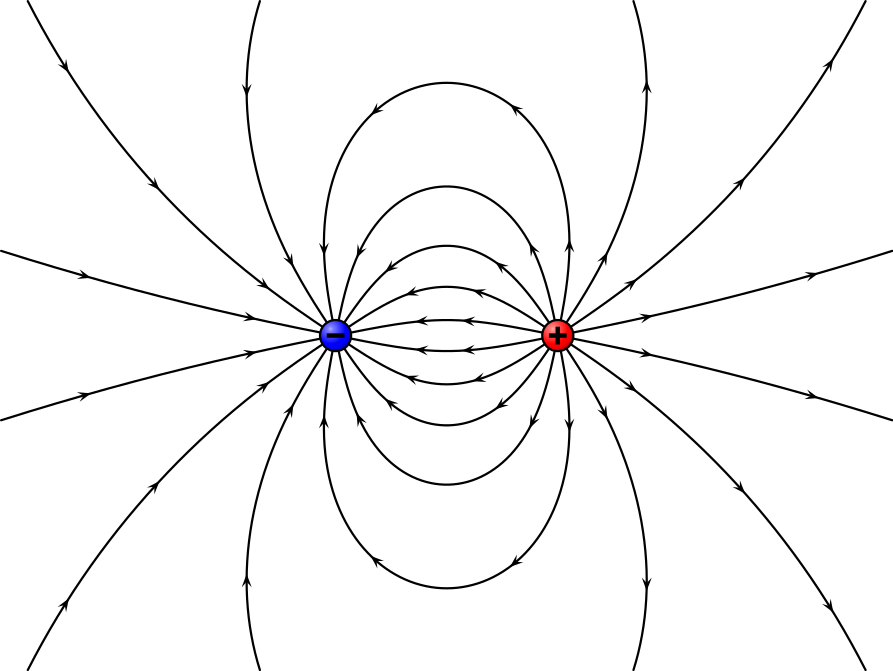
\includegraphics[height=4cm]{fig/fig-E-02.pdf}\hspace{1cm}\includegraphics[height=4cm]{fig/fig-campo-dipolo-electrico.pdf} 
\caption{Dipolo (dos cargas opuestas) versus dipolo ideal. Figuras creadas usando VectorFieldPlot \cite{VFP}.}
\label{fig-dipolos}
\end{center}
\end{figure}
\subsubsection{Cuadrupolo ideal}
$Q=0$ $p_i=0$, $Q_{ij}\neq 0$, $Q_{ijk}=0$, etc.

\begin{figure}[H]
\begin{center}
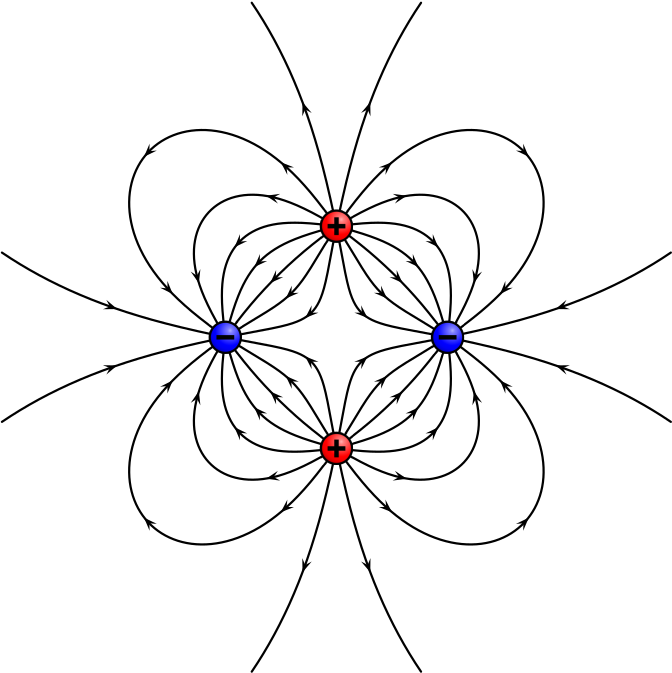
\includegraphics[height=4cm]{fig/fig-E-03.pdf}\hspace{1cm}\includegraphics[height=4cm]{fig/fig-campo-cuadrupolo-electrico-ideal.pdf} 
\caption{Cuadrupolo versus cuadrupolo ideal. Figuras creadas usando VectorFieldPlot \cite{VFP}.}
\label{fig-dipolos2}
\end{center}
\end{figure}
\newpage


\subsection{Distribuciones de carga en campos externos} \label{ed3_3}

En las secciones anteriores hemos considerado la expansión multipolar
\textit{generada} por una distribución compacta de carga
$\rho(\vec{x})$. Ahora discutiremos una situación distinta: consideraremos
una (pequeña) distribución de cargas en un campo eléctrico
\textit{externo} (es decir, generado por alguna \textit{otra} distribución de
carga). En particular, calcularemos la energía potencial de la
distribución de carga en el campo externo dado, así como la fuerza y el
torque que el campo externo ejerce.

\subsubsection{Energía Potencial} \label{ed3_3_1}


Para evaluar esta integral, consideramos un \textit{punto representativo $P$ de la
distribución} con coordenadas $\vec{x}$ y un punto $P'$ cualquiera de la
distribución  (con coordenadas $\vec{x}+\vec{x}'$ respecto
al origen, ver figura) determinado por el vector $\vec{x}'$ respecto al punto
representativo $P$ de la distribución, y expandiremos los valores $\phi(P')$ en
una serie de Taylor en torno a $P$:
\begin{align} \label{eq3.3.3}
\phi(P') = &\ \phi(\vec{x}+\vec{x}')\\
= & \sum_{n=0}^\infty\frac{1}{n!}x'_{i_1}\cdots
x'_{i_n}\left.(\partial_{i_1}\cdots\partial_{i_n}\phi)\right|_{\vec{x}'=\vec{0}} \\
= &\ \left.\phi\right|_{\vec{x}'=\vec{0}}+x'_i\left.(\partial_i\phi)\right|_{\vec{
x}'=\vec{0}}+\frac{1}{2}x'_ix'_j\left.(\partial_i\partial_j\phi)\right|_{\vec{x}
'=\vec{0}}+\cdots \nonumber\\
& +\frac{1}{n!}x'_{i_1}\cdots
x'_{i_n}\left.(\partial_{i_1}\cdots\partial_{i_n}\phi)\right|_{\vec{x}'=\vec{0}}
+\cdots\\
= &\ \phi(\vec{x})-x'_iE_i(\vec{x})-\frac{1}{2}x'_ix'_j(\partial_iE_j)(\vec{x}
) \nonumber \\
& -\cdots-\frac{1}{n!}x'_{i_1}\cdots
x'_{i_n}(\partial_{i_1}\cdots\partial_{i_{n-1}}E_{i_n})(\vec{x})+\cdots .
\end{align}

Con esto, podemos escribir (\ref{Urhophiext}) como
\begin{eqnarray}
 U&=&\int\rho(P')\,\phi(P')\,dV'\\
&=&\sum_{n=0}^\infty\frac{1}{n!}\left[\int\rho(P')x'_{i_1}\cdots
x'_{i_n}\,dV'\right]\left.(\partial_{i_1}\cdots\partial_{i_n}\phi)\right|_{\vec{x}'=\vec{0}}\\
%&=&\left[\int\rho(\vec{x}')
%\phi(\vec{x})-\left[\int\rho(\vec{x}')\,
%x'_i\,dV'\right] E_i(\vec{x})-\frac{1}{2}\left[ \int\rho(\vec{x}')\,
%x'_ix'_j\,dV'\right](\partial_iE_j)(\vec{x})
%\nonumber\\
%&&-\cdots-\frac{1}{n!}\left[ \int\rho(\vec{x }')\, x'_{i_1}\cdots
%x'_{i_n}\,dV'\right] (\partial_{i_1}
%\cdots\partial_{i_{n-1}}E_{i_n})(\vec{x})+\cdots \\
&=&\sum_{n=0}^\infty\frac{1}{n!}Q_{i_1\cdots i_n}(\partial_{i_1}\cdots\partial_{i_n}\phi)(\vec{x})\\
&=&Q\phi(\vec{x})-Q_iE_i(\vec{x})-\frac{1}{2}
Q_{ij}(\partial_iE_j)(\vec{x}) \nonumber \\
&& -\cdots-\frac{1}{n!}Q_{i_1\cdots i_n}(\partial_{i_1}
\cdots\partial_{i_{n-1}}E_{i_n})(\vec{x})+\cdots .
\end{eqnarray}
Por lo tanto, obtenemos que la energía potencial de una distribución de
carga, caracterizada por sus momentos multipolares, en un \textit{campo externo}
es dado por
\begin{equation} \label{eq3.3.4}
\boxed{U=Q\,\phi(\vec{x})-\vec{p}\cdot\vec{E}(\vec{x})-\frac{1}{2}\,Q_{ij}
\,\partial_iE_j(\vec{x})+\cdots .}
\end{equation}

El primer término de esta expansión, la contribución monopolar, es
equivalente a la de una carga \textit{puntual} en un potencial externo. El
término siguiente (dipolar) representa la energía potencial de un dipolo
ideal en un campo eléctrico externo. Note que este término es mínimo cuando
el momento dipolar es paralelo al campo eléctrico externo (y es, en general,
proporcional al coseno del ángulo entre $\vec{p}$ y $\vec{E}$). El término
cuadrupolar es distinto de cero sólo cuando el campo es inhomogéneo. Note que
en esta expresión también es posible usar un momento cuadrupolar redefinido
como se discutió en la sección (\ref{MCSM}). En particular puede usarse el
momento cuadrupolar sin traza. La energía potencial calculada usando distintos
momentos cuadrupolares equivalentes es la misma puesto que un término
proporcional a $\delta_{ij}$ contribuira con un término proporcional a
$\delta_{ij}(\partial_iE_j)=\partial_iE_i$, que es cero en virtud de la ley de
Gauss y el hecho que $\vec{E}$ describe un \textit{campo eléctrico externo},
es decir, un campo generados por fuentes fuera de la región bajo
consideración.


\subsubsection{Fuerza}  \label{ed3_3_2}

Una carga puntual $q$ experimenta una fuerza
$\vec{F}(\vec{x})=q\,\vec{E}(\vec{x})$ cuando está situada en
un punto donde existe un campo externo $\vec{E}(\vec{x})$. Como consecuencia,
la fuerza total sobre una distribución con densidad $\rho$ en un campo
\textit{externo} puede escribirse como
\begin{equation} \label{eq3.3.7}
F_i=\int \rho(P')\,E_i(P')\,dV'.
\end{equation}
Expandimos $E_i(P')$ en serie de Taylor, de forma similar a como lo
hicimos en la sección anterior con el potencial
\begin{equation} \label{eq3.3.7.1}
E_i(P')=E_i(\vec{x})+x'_j(\partial_jE_i)(\vec{x})+\frac{1}{
2}x'_jx'_k(\partial_j\partial_kE_i)(\vec{x})
+\cdots+\frac{1}{n!}x'_{i_1}\cdots
x'_{i_n}(\partial_{i_1}\cdots\partial_{i_n}E_i)(\vec {x})+\cdots .
\end{equation}
Con esto, podemos reescribir (\ref{eq3.3.7}) como
\begin{eqnarray}
F_i&=& \int
\rho(P')\,\left[E_i(\vec{x})+x'_j(\partial_jE_i)(\vec{x})+\frac{1}{
2}x'_jx'_k(\partial_j\partial_kE_i)(\vec{x}) \right.\nonumber\\
&& \quad\qquad\qquad \left. +\cdots+\frac{1}{n!}x'_{i_1}\cdots
x'_{i_n}(\partial_{i_1}\cdots\partial_{i_n}E_i)(\vec {x})+\cdots\right] dV' \\
&=&
Q\,E_i(\vec{x})+p_j(\partial_jE_i)(\vec{x})+\cdots+\frac{1}{n!}Q_{i_1\cdots i_n}
(\partial_{i_1}\cdots\partial_{i_n}E_i)(\vec {x})+\cdots .\label{eq3.3.8}
\end{eqnarray}
El primer término, $Q\vec{E}(\vec{x})$, es nuevamente la contribución monopolar correspondiente a la fuerza sobre una carga puntual. La contribución
dipolar es ahora proporcional al gradiente del campo eléctrico. Usando el hecho que el campo electrostático satisface
$\partial_iE_j=\partial_jE_i$ podemos expresar el término dipolar como $\partial_i(p_jE_j)$,
es decir.
\begin{equation} \label{eq3.3.12}
\boxed{\vec{F}(\vec{x}) =
Q\vec{E}(\vec{x})-\vec{\nabla}\left(-\vec{p}\cdot\vec{E}(\vec{x})\right)+\cdots.
}
\end{equation}
Note que el segundo término es el gradiente de la contribución dipolar a la
energía potencial de la distribución.

\subsubsection{Torque}  \label{ed3_3_3}

Análogamente al caso de la fuerza total, podemos calcular el \textit{torque
neto} ejercido por el campo externo sobre la distribución, respecto del punto
representativo que hemos considerado:
\begin{equation}
\vec{\tau} = \int \rho(P')\,\vec{x}'\times\vec{E}(P')\,dV' .
\end{equation}
En componentes, y usando la expansión (\ref{eq3.3.7.1}) obtenemos
\begin{eqnarray}
\tau_i &=& \varepsilon_{ijk}\int\rho(P')x'_jE_k(P')\,dV' \\
&=&\varepsilon_{ijk}\int\rho(P')x'_j\left[
E_k(\vec{x})+x'_l(\partial_lE_k)(\vec{x})+\frac{1}{2}
x'_lx'_m(\partial_l\partial_mE_k)(\vec{x}) \right.\nonumber\\
&&\quad\qquad\qquad\qquad\left.+\cdots+\frac{1}{n!}x'_{i_1}\cdots
x'_{i_n}(\partial_{i_1}\cdots\partial_{i_n}E_k)(\vec
{x})+\cdots\right] \,dV' \\
&=&\varepsilon_{ijk}\left[p_j
E_k(\vec{x})+Q_{jl}(\partial_lE_k)(\vec{x})+\frac{1}{2}
Q_{jlm}(\partial_l\partial_mE_k)(\vec{x})\right.\nonumber\\
&&\quad\qquad\qquad\qquad\left.+\cdots+\frac{1}{n!}Q_{ji_1\cdots i_n}(\partial_{i_1}\cdots\partial_{i_n}
E_k)(\vec
{x})+\cdots\right] .
\end{eqnarray}
Por lo tanto,
\begin{equation}
\label{eq3.3.14}
\boxed{\vec{\tau}=\vec{p}\times\vec{E}(\vec{x})+\cdots. }
\end{equation}
Es posible expresar la primera contribución (dipolar) al torque como un
``gradiente'' del término dipolar de la energía potencial
$U_{\vec{p}}=-\vec{p}\cdot\vec{E}$, esta vez, sin embargo, no respecto a
variaciones de la posición $\vec{x}$ de la distribución, sino con respecto a
cambios en la orientación del momento dipolar respecto al campo
externo. La magnitud del torque es dada por
\begin{eqnarray}
\tau &=& pE\sin\theta \nonumber \\
&=& -\frac{d}{d\theta}\,\left(pE\cos\theta\right)\\
&=&\frac{dU_{\vec{p}}}{d\theta}.  \label{eq3.3.15}
\end{eqnarray}

\newpage


\newpage

\section{Electrostática macroscópica}
Hasta ahora hemos estudiado las propiedades de los campos
electrostáticos \textit{en el vacío} y en el interior de \textit{condutores ideales}.
Estamos ahora interesados en las propiedades el campo eléctrico \textit{macroscópico} en el interior de un material \textit{aislante}. El término macroscópico se refiere al campo promedio en una pequeña región que, sin embargo, es grande comparada con el tamaño de las moléculas que constituyen el material.

Consideraremos entonces materiales aislantes, también llamados \textit{dieléctricos}, en los que las cargas internas no tienen la
libertad de desplazarse distancias macroscópicas (conducir) en presencia de un
campo eléctrico aplicado, sino que están confinadas por la estructura
atómica/molecular del material. La mayoría de los materiales son, en buena
aproximación, dieléctricos.

En presencia de un campo eléctrico los dieléctricos \textit{redistribuyen sus cargas} constituyentes. éstas no pueden desplazarse distancias macroscópicas,
como ocurre en los conductores, sino sólo distancias del orden de magnitud determinado por su estructura molecular.
Estos pequeños desplazamientos de carga tienen, sin embargo, consecuencias
que se acumulan hasta ser perceptibles a escalas macroscópicas.
Concretamente, en presencia de un campo eléctrico, el material
se \textit{polariza}.
El campo eléctrico que causa (el cambio en) la polarización puede ser un campo ``externo'' (producido por ``cargas externas''\footnote{También llamadas ``cargas libres'' o ``cargas no ligadas''.}, que no forman parte
de la estructura atómica/molecular característica del medio).
\begin{figure}[!h]
\centerline{\includegraphics[height=4cm]{fig/fig-dielectrico-01.pdf}}
\caption{Un material dieléctrico se polariza en presencia de un campo externo.}
\label{diel01}
\end{figure}

El campo eléctrico total (``EL''\, campo eléctrico) es influenciado por
la polarización del medio. Modelaremos este campo eléctrico
(macroscópico) $\vec{E}$ como la suma del campo
producido por las cargas externas y el campo producido por la distribución
de \textit{cargas de polarización} (descrita por el vector de polarización $\vec{P}$) del medio.

\subsection{Vector y cargas de Polarización}

Se define el \textit{vector de polarización} como la \textit{densidad de
momento dipolar} (momento dipolar por unidad de volumen),
\begin{equation}\label{defP}
\vec{P}(x):= ``\lim_{\Delta V\to 0}" \frac{\Delta\vec{p}}{\Delta V},
\end{equation}
donde $\Delta\vec{p}$ es el \textit{momento dipolar total de las cargas del material contenidas en el volumen} $\Delta V$. La región con volumen $\Delta V$ se considera centrada en el punto $\vec{x}$, suficientemente pequeña desde el punto de vista macroscópico, pero grande comparada con la escala  determinada por la estructura atómica/molecular del material. Equivalentemente, el vector de polarización es definido tal que el momento dipolar $d\vec{p}$ en un elemento de volumen (macroscópico) $dV$ es dado por $d\vec{p}=\vec{P}(\vec{x})dV$.

Como consecuencia de la definición anterior, el momento dipolar
total de las cargas contenidas en un volumen finito $V$ es dado por
\begin{equation}\label{pintPdV}
 \vec{p}_V=\int_V \vec{P}(x)\,dV.
\end{equation}
Por otro lado, sabemos que el potencial generado por un dipolo ideal de momento dipolar $\vec{p}$ ubicado en un punto con coordenadas $\vec{x}'$ es de la forma \eqref{phip}. Luego, el potencial generado por una pequeña región de un medio polarizado con elemento de volumen $dV'$ y polarización $\vec{P}$ es dada por
\begin{equation}
d\phi(x)=\frac{1}{4\pi\varepsilon_0}\frac{(x_j-x_j')P_j(x')\,dV'}{|\vec{x}-\vec{
x}'|^3}.
\end{equation}
De esta forma, si el sistema contiene además cargas libres en $dV'$ entonces
\begin{equation}
d\phi(x)=\frac{1}{4\pi\varepsilon_0}\frac{\rho_{\rm
ext}(x')}{|\vec{x}-\vec{x}'|}dV'+\frac {1}{
4\pi\varepsilon_0}\frac{P_i(x')(x_i-x_i')}{|\vec{x}-\vec{x}'|^3}dV'.
\end{equation}
Por lo tanto, el potencial (macroscópico, total), de acuerdo a nuestro modelo, es dado por
\begin{equation}
\boxed{\phi(x)=\frac{1}{4\pi\varepsilon_0}\int\left[\frac{\rho_{\rm
ext}(x')}{|\vec{x}-\vec{x}'|}+\frac{P_i(x')(x_i-x_i')}{|\vec{x}-\vec{x}'|^3}\right]dV'.}
\end{equation}
Usando la identidad (\ref{id01}) podemos escribir
\begin{align}
\frac{P_i(x')(x_i-x_i')}{|\vec{x}-\vec{x}'|^3}  &
=P_i(x')\partial_i'\left(  \frac{1}{|\vec{x}-\vec{x}'|}\right)\\
&=\partial_i'\left(\frac{P_i(x')}{|\vec{x}-\vec{x}'|}\right)-\frac{
(\partial_i'P'_i)(x')} {|\vec{x}-\vec{ x}'|}.
\end{align}
De esta forma, considerando que la integral sobre los términos que dependen de la polarización están confinados al volumen $V$ del material (lo que no necesariamente es así para el término conteniendo las cargas libres), podemos escribir
\begin{align}
\phi(x)& =\frac{1}{4\pi\varepsilon_0}\int\frac{\rho_{\rm ext}(x')}{|x_i-x_i'|}dV'-\frac{1}{4\pi\varepsilon_0}\int_V\frac{1}
{|\vec{x}-\vec{x}'|}\partial_i'P_idV'+\frac{1}{4\pi\varepsilon_0}\int_{
\partial V}\frac{P_i(x')}{|\vec{x}-\vec{x}'|}\,dS'_i \\
& =\frac{1}{4\pi\varepsilon_0}\int\frac{\rho_{\rm ext}(x')}{|x_i-x_i'|}dV'+\frac{1}{4\pi\varepsilon_0}\int_V\frac{\rho_P(x')}{|x_i-x_i'|}dV'+\frac{1}{4\pi\varepsilon_0}\int_{
\partial V}\frac{\sigma_P(x')}{|\vec{x}-\vec{x}'|}\,dS' .
\end{align}
La expresión anterior muestra que el campo (macroscópico) total es
\textit{equivalente} al campo producido por una densidad volumétrica de carga total,
\begin{equation}
\rho_{\rm T}:=\rho_{\rm ext}+\rho_P, \label{rhotot}
\end{equation}
donde
\begin{equation}
\boxed{\rho_P:=-\vec{\nabla}\cdot\vec{P},}
\end{equation}
es la \textit{densidad (volumétrica) de carga de polarización}, (definida en cada punto del material), más una
\textit{densidad de carga de polarización de superficie},
\begin{equation}
\boxed{\sigma_P:=\vec{P}\cdot\hat{n},}
\end{equation}
distribuida en la superficie $S=\partial V$ del dieléctrico.

Note que la carga total de polarización, tal como se espera, es nula:
\begin{equation}
 Q_P=\int_V\rho_P\,dV+\oint_{\partial V} \sigma_P\,dS\equiv 0,
\end{equation}
en virtud del teorema de Gauss.

\subsection{Desplazamiento eléctrico}
Usando (\ref{rhotot}) en la ley de Gauss, podemos escribir
\begin{align*}
\vec\nabla\cdot\vec{E} &=\frac{1}{\varepsilon_0}\rho_T \\
&=\frac{1}{\varepsilon_0}\left( \rho_{\rm ext}-\vec\nabla\cdot\vec{P}\right).
\end{align*}
Luego,
\begin{equation}
 \vec\nabla\cdot\left(\vec{E}+\frac{1}{\varepsilon_0}\vec{P}\right)=\frac{\rho_{
\rm ext}(x)}{\varepsilon_0}.
\end{equation}
Definimos el \textit{vector de desplazamiento eléctrico} (también llamado
\textit{excitación eléctrica} o \textit{inducción eléctrica}) como
\begin{equation}\marginnote{Vector Desplazamiento}
 \boxed{\vec{D}(\vec{x}):=\varepsilon_0\vec{E}(\vec{x})+\vec{P}(\vec{x}),} \label{defD}
\end{equation}
de modo que
\begin{equation}
\boxed{\vec{\nabla}\cdot\vec{D}=\rho_{\rm ext}.} \label{divD}
\end{equation}
Las unidades del vector desplazamiento son de carga por unidad de área: 
$[\vec{D}]=[\vec{P}]=[\sigma]\stackrel{\text{
S.I.}}{=}{C}/{m^2}$.

La utilidad de usar $\vec{D}$ en lugar de $\vec{E}$ en esta ``ley de Gauss"
\,\eqref{divD} es que esta relación \textit{sólo involucra explícitamente a las cargas externas} (que son usualmente conocidas y/o controlables). Por ejemplo, como consecuencia de (\ref{divD}) tenemos que
\begin{equation}
 \boxed{\oint_S \vec{D}\cdot d\vec{S}=q_{\rm ext}.} \label{GaussD}
\end{equation}

\subsubsection{Ejemplo: Esfera dieléctrica isótropa y carga central}
\begin{figure}[!h]
\centerline{\includegraphics[height=4cm]{fig/fig-dielectrico-y-carga-01.pdf}}
\caption{Un material dieléctrico isótropo con una carga central.}
\label{diel02}
\end{figure}
Consideremos una carga (externa) $Q$ situada en el centro de una
esfera dieléctrica \textit{isótropa}, ver figura \ref{diel02}, podemos encontrar el vector de desplazamiento aplicando (\ref{GaussD}). Debido a la simetría del sistema (ya que asumimos que el dieléctrico es \textit{isótropo}, ver secciones \ref{sec:aniso} y \ref{sec:iso}), tendremos que $\vec{D}(\vec{x})=D(r)\hat{r}$. Eligiendo una superficie Gaussiana esférica de radio $r$ centrada en la carga $Q$, encontramos entonces que
\begin{equation}
 D(r)\oint_S dS=D(r)4\pi r^2=Q,
\end{equation}
y por lo tanto
\begin{equation}
 \vec{D}(\vec{x})=\frac{Q}{4\pi}\frac{1}{r^2}\,\hat{r}.
\end{equation}


\subsection{Relación Constitutiva, susceptibilidad, permeabilidad}

Cada medio se caracteriza por la polarización $\vec{P}(\vec{x})$ que presenta,
dados los campos/cargas externas. Esta polarización $\vec{P}(\vec{x})$ depende
entonces de los campos/cargas externas y de la constitución atómica/molecular
del material (y en principio de otras propiedades, como la temperatura,
presión, etc). 
%Equivalentemente, esta información acerca de las propiedades
%del material puede expresarse en la relación entre el campo eléctrico
%$\vec{E}(\vec{x})$ y el vector desplazamiento eléctrico $\vec{D}(\vec{x})$.

En un elemento de volumen dado del medio éste modificará su distribución microscópica de cargas como respuesta al campo eléctrico ``total"\,que actúa sobre este elemento, hasta finalmente adoptar un cierta polarización. Podemos, por tanto, considerar que $\vec{P}=\vec{P}(\vec{E})$ o, equivalentemente
$\vec{D}=\vec{D}(\vec{E})$. Esta última relación es llamada
\textit{relación constitutiva} del medio. El problema es que el campo
$\vec{E}(\vec{x})$ en un punto dado (con vector de polarización $\vec{P}(\vec{x})$ y
por tanto desplazamiento $\vec{D}(\vec{x})$) depende también de cómo se
polariza el medio \textit{en otras regiones}, e.d., $\vec{E}(\vec{x})$ depende
en general de\footnote{Matemáticamente, esto significa que, en
general, $\vec{E}$ es un \textit{funcional}, una ``función de funciones''\, o
una ``función no-local''\, de $\vec{P}$.} $\vec{P}(\vec{x}')$.
En otras palabras, en general la polarización que se presentará en un medio es fruto de la  \textit{respuesta colectiva} del material a los campos externos.

 Vemos entonces que calcular $\vec{P}(\vec{x})$ desde ``primeros principios'' es en gerenal difícil y requiere conocer los detalles de la estructura del material en estudio.

Existe una gran variedad de medios materiales con propiedades eléctricas
diferentes e interesantes. Existen por ejemplo medios que tienen \textit{polarización
no nula aún en ausencia de campos/cargas externas}. Estos medios son conocidos
como \textit{electretos} (análogos eléctricos de los imánes permanentes), y 
\textit{ferroeléctricos} (que presentan polarización no nula bajo una cierta
temperatura crítica, de Curie, análogamente a los ferromagnetos). Un ejemplo
de material ferroeléctrico es el $BaTiO_3$ (\href{https://en.wikipedia.org/wiki/Barium_titanate}{titanato de bario}), que exhibe un momento dipolar eléctrico no nulo a temperaturas bajo $120^{\rm o}\,C$. Un ejemplo de electreto es el cuarzo ($SiO_2$, \href{https://en.wikipedia.org/wiki/Silicon_dioxide}{dióxido de Silicio}), que presenta \href{https://es.wikipedia.org/wiki/Piezoelectricidad}{\textit{propiedades piezoeléctricas}}.

Es útil además distinguir entre distintos tipos de polarización, dependiendo del mecanismo que gobierne dicha propiedad: \textit{polarización electrónica}, p.ej. cuando un átomo se ``deforma"\,en presencia de un campo externo; \textit{polarización iónica}, causada por arreglo de iones (p.ej. $NaCl$); \textit{polarización polar} que se manifiesta en los gases (cuando la
temperatura aumenta, disminuye la polarización porque las moléculas se
``desordenan").

Más aún, en algunos materiales (``no-lineales''\,) la respuesta
(polarización) del material puede depender no-linealmente del campo eléctrico.

Sin embargo, existe una gran variedad de materiales que, desde el punto de
vista macroscópico, pueden ser modelados adecuadamente (es decir, con \textit{precisión suficiente} en la mayoría de las situaciones) por una relación lineal entre $\vec{D}$ y $\vec{E}$. Un \textit{material lineal}, pero en general \textit{no-local}, puede describirse a
través de una relación de la forma
\begin{equation}
D_i[\vec{E}](\vec{x},t)=\int
f_{ij}(\vec{x},\vec{x}',t,t')\,{E}_j(\vec{x}',t')\,dV' dt',
\end{equation}
donde $f_{ij}(\vec{x},\vec{x}',t,t')$ es un cierto tensor que describe las
propiedades del medio. Como la polarización y por tanto el vector
desplazamiento en un punto $\vec{x}$ del medio están influenciadas en forma
más determinante por lo que le ocurre al material en la inmediata vecindad de
$\vec{x}$ es de esperar que la función $f_{ij}(\vec{x},\vec{x}',t,t')$ sea
concentrada en torno a $\vec{x}$, es decir, que decaiga rápidamente para
$|\vec{x}'-\vec{x}|\gg d$ donde $d$ es la escala característica de la
estructura microscópica del medio.

Por otro lado, existen muchos casos en que es \textit{suficiente} considerar una
\textit{relación constitutiva local} en la que el vector desplazamiento en un
punto dado puede modelarse como dependiendo exclusivamente del valor del campo
eléctrico \textit{en el mismo punto} (macroscópico), es decir
$\vec{D}(\vec{x})=\vec{D}(\vec{E}(\vec{x}))$ o, equivalentemente
$\vec{P}(\vec{x})=\vec{P}(\vec{E}(\vec{x}))$.

En un material descrito por una relación constitutiva local podemos considerar
la dependencia de $\vec{P}$ con $\vec{E}$ a través de una expansión en serie
de la forma:
\begin{equation}\label{expP}
P_i(x)=P_i(E_j(x))=(P_i)_{\vec{E}=\vec{0}}
+E_j(\partial_jP_i)_{\vec{E}=\vec{0}}+\frac{1}{2}
E_jE_k(\partial_j\partial_k P_i)_{\vec{E}=\vec{0}}+\cdots,
\end{equation}
que esperamos sea útil para campos eléctricos suficientemente débiles (en el
presente contexto sólo podemos saber \textit{a posteriori} qué tan débil
requiere ser el campo). Note que en el lado derecho de (\ref{expP}) las derivadas $\partial_i$ denotan derivadas respecto a la componente $i$-ésima del campo eléctrico, es decir $\partial_iP_j={\partial P_j}/{\partial E_i}$, etc.. Las cantidades $(P_i)_{\vec{E}=\vec{0}}$,
$(\partial_jP_i)_{\vec{E}=\vec{0}}$,
$(\partial_j\partial_k P_i)_{\vec{E}=\vec{0}}$, etc. son
tensores (cartesianos) que asumen diferentes valores para cada material y pueden ser
considerados como parámetros (a determinar). Con esto, podemos escribir
\begin{equation}
\boxed{P_i(x)={\cal A}_i+{\cal A}_{ij}E_j+{\cal A}_{ijk}
E_jE_k+\cdots.}
\end{equation}
En general, si el material es \textit{inhomogéneo} (por ejempo, si está formado por
capas de distintos materiales), los tensores ${\cal A}_i$, ${\cal A}_{ij}$, ${\cal A}_{ijk}$, etc. dependerán de la posición. Para materiales no-ferroeléctricos (la gran mayoría) tenemos que ${\cal A}_i=0$.



\subsection{Medios lineales anisótropos}\label{sec:aniso}

Adicionalmente, si la polarización de un material es descrita apropiadamente
por una relación lineal, como ocurre en el caso de campos eléctricos
suficientemente débiles, tendremos
\begin{equation}
\boxed{P_i(x)=\varepsilon_0\chi_{ij}(x)E_j(x),} \label{rcml}
\end{equation}
entonces decimos que el medio es \textit{lineal}. El tensor $\chi_{ij}$ es
llamado \textit{tensor de susceptibilidad eléctrica} del medio.  El factor $\varepsilon_0$ es incluido de modo que $\chi_{ij}$ es un tensor adimensional. En este caso,
usando (\ref{defD}) y (\ref{rcml}), tenemos que
\begin{equation}\label{rclai}
\boxed{D_i(x)=\varepsilon_{ij}(x)E_j(x)=\varepsilon_0\,\kappa_{ij}(x)E_j(x),}
\end{equation}
donde hemos definido el \textit{tensor de permitividad} del medio
$\varepsilon_{ij}$, por
\begin{equation}
\varepsilon_{ij}:=\varepsilon_0(\delta_{ij}+\chi_{ij})
\end{equation}
y, alternativamente,  el \textit{tensor dieléctrico},
\begin{equation}
\kappa_{ij}:=\frac{1}{\varepsilon_0}\varepsilon_{ij}=\delta_{ij}+\chi_{ij},
\end{equation}
que tiene la ventaja de ser una cantidad adimensional.

Es posible probar por
argumentos energéticos que si el medio no es disipativo (no existen mecanismos
de transferencia de energía del campo eléctrico a otras formas de energía)
entonces necesariamente $\chi_{ij}$ (y por tanto $\varepsilon_{ij}$ y
$\kappa_{ij}$) es un tensor \textit{simétrico} y que posee, por lo
tanto, 6 componentes independientes. La descripción de las
propiedades de un medio lineal a través de un tensor de susceptibilidad
eléctrica incluye el caso en que el medio sea \textit{anisótropo}, es decir,
que sus propiedades no sean invariantes bajo rotaciones o, en otras palabras,
que posea ciertas \textit{direcciones preferentes}. En un medio anisótropo, la
polarización no será en general paralela al campo eléctrico (excepto para las
direcciones preferentes dadas por las direcciones principales. Ver sección
\ref{secDP}.), esto como
resultado de la estructura microscópica del material (típicamente, cristales),
que tienen como consecuencia que el material se polarize en algunas direcciones
más fácilmente que en otras.


Note que en el caso más general en que se consideran campos eléctricos dependientes del tiempo (esto es necesario, por ejemplo, en el caso de propagación de ondas electromagnéticas), aún cuando un medio pueda considerarse lineal y local respecto a su dependencia con la posición, la relación constitutiva es de la forma
\begin{equation}
D_i(x,t)=\int f_{ij}(t,t')E_j(x,t')\,dt'.
\end{equation}
En estos casos es conveniente considerar las \textit{transformadas de Fourier temporal} de los campos, es decir $\tilde{D}_i(x,\omega)$, $\tilde{E}_i(x,\omega)$, etc., ya que permiten escribir la relación constitutiva como
\begin{equation}\label{RELtilde}
\tilde{D}_i(x,\omega)=\tilde{\varepsilon}_{ij}(x,\omega)\tilde{E}_j(x,\omega). 
\end{equation}
Comparando \eqref{RELtilde} con \eqref{rclai} vemos que en el caso más general, el tensor $\tilde{\varepsilon}_{ij}(x,\omega)$ juega un rol análogo a $\varepsilon_{ij}$ en \eqref{rclai} y también es llamado, por esta razón, el tensor dieléctrico del medio. Note, sin embargo, que este tensor \textit{asume valores complejos y depende en general de la frecuencia} $\omega$.


\subsection{Medios lineales isótropos}\label{sec:iso}
Si el material es isótropo, es decir, si éste no posee ninguna dirección
preferente, la polarización debe necesariamente ser paralela al campo
eléctrico, independientemente de la dirección de este último. Esta condición requiere que el tensor de susceptibilidad sea proporcional al tensor identidad,
\begin{equation}
\chi_{ij}=\chi\,\delta_{ij},
\end{equation}
de modo que
\begin{equation}
\vec{P}=\varepsilon_0\chi\vec{E}.
\end{equation}
Muchos materiales presentan propiedades de polarización independientes de
la dirección del campo eléctrico, es decir, son isótropos. Por ejemplo, los
gases, líquidos (excepto los, así llamados, \textit{cristales liquidos}), sólidos amorfos (plásticos, vidrio).
Los medios no-lineales, pero isótropos, pueden ser descritos usando
$\vec{P}=\varepsilon_0\chi(|\vec{E}|)\vec{E}$.

En este curso, a menos que se explicite lo contrario, consideramos siempre
materiales lineales, isótropos y homogéneos. En este caso, es suficiente
introducir la (``constante de''\,) permitividad y/o la constante dieléctrica
por
\begin{equation}
\varepsilon:=\varepsilon_0(1+\chi), \qquad
\kappa:=\frac{\varepsilon}{\varepsilon_0}=1+\chi.
\end{equation}
Note que en un medio polarizable es de esperar que $\chi>0$, de modo que
$\varepsilon>\varepsilon_0$ o, equivalentemente, $\kappa>1$. El vacío puede ser
considerado como un ``medio isótropo''\, con $\chi=0$ y $\kappa=1$, es decir, no polarizable.
Recuerde también que el índice de refracción de la mayoría de los medios
(``no-magnéticos''\,) es dado por $n\approx\sqrt{\kappa}$.
\begin{table}[!h]
\begin{center}
\begin{tabular}{c|c}
Material &   $\kappa$ \\ \hline\hline
Vacío & 1 \\
Aire (seco, $0^{\rm o}$C, 1 bar)  & 1,00059 \\
Agua ($110^{\rm o}$C, 1 bar)  & 1,0126 \\
Agua ($20^{\rm o}$C) &  80,0 \\
Hielo ($-30^{\rm o}$C) &  99 \\
$SrTiO_3$ (cristal, $10$K)  & 12.000 \\
\end{tabular}
\caption{Algunos materiales isótropos y sus constantes dieléctricas.}
\end{center}
\end{table}

\subsection{Ecuación de Poisson y su generalización}

Usando (\ref{divD}) y (\ref{E=nablaphi}) encontramos la generalización de la
ecuación de Poisson para el potencial en un dieléctrico lineal y local:
\begin{equation}
 \boxed{\partial_i\left(\kappa_{ij}\,\partial_j \phi\right)
=-\frac{1}{\varepsilon_0}\rho_{\rm ext}.}
\end{equation}
Para un material homogéneo e isótropo, esta ecuación se reduce a
\begin{equation}\label{Poissond}
 \boxed{\nabla^2\phi=-\frac{1}{\varepsilon}\rho_{\rm ext},}
\end{equation}
que tiene la misma forma (matemáticamente, es la \textit{misma} ecuación) que
en caso del campo en el vacío ($\varepsilon=\varepsilon_0$). Finalmente, en
regiones fuera de cargas externas (!`\,pero \textit{no} de cargas de
polarización!), el potencial satisface la ecuación de Laplace. Como
consecuencia, es posible usar las técnicas conocidas para solucionar esta ecuación, por ejemplo, expansión en funciones especiales, o funciones de Green, en el caso de los dieléctricos.
Como veremos a continuación, una diferencia importante respecto al caso en el
vacío será la implementación de las condiciones de borde o frontera.


\subsection{Direcciones principales de un medio anisótropo}\label{secDP}

Como vimos, en un medio anisótropo, el campo eléctrico no tiene en general
la misma dirección que el vector desplazamiento.
Existen, sin embargo, direcciones ``especiales''\, a lo largo de las cuales el
campo eléctrico sí tiene la misma dirección que la polarización. Esto significa
que, si $\hat{n}$ es una de estas direcciones, conocidas como \textit{direcciones
principales} del material, entonces $\vec{E}=E\hat{n}$ y $\vec{D}=D\hat{n}$.
Insertando estas condiciones en (\ref{rclai}) obtenemos que
\begin{equation}
\kappa_{ij}\,\hat{n}_j= \lambda\,\hat{n}_i, \qquad D=\varepsilon_0\lambda E.
\end{equation}
Vemos de aquí que las direcciones principales corresponden a los vectores
propios de la matriz  $\kappa_{ij}$, mientras que el valor propio $\lambda$ es
el valor de la constante dieléctrica del material a lo largo de aquella
dirección principal. Como la matriz $\kappa_{ij}$ es real y simétrica, es
posible encontrar tres vectores propios ortonormales, es decir, una base
ortonormal formada por las direcciones principales del material. Existen
distintos casos particulares e interesantes de materiales anisótropos
correspondiendo a si los valores propios son todos diferentes o iguales. Si
todos los valores propios son iguales, el material es isótropo, puesto que en
ese caso $\kappa_{ij}=\lambda\,\delta_{ij}$. Si dos valores propios son iguales
y uno diferente, se dice que el material es \textit{uniaxial} (puesto que
tienen una dirección distintiva, aquella descrita por el vector propio del
valor propio distinto a los otros dos. Esta dirección es llamada \textit{eje
óptico}). Un ejemplo de material uniaxial natural es la Calcita ($CaCO_3$). En
materiales uniaxiales la propagación de la luz presenta el fenómeno llamado
\textit{birefringencia}, en los que la luz en su interior se propaga, en
general, por dos trayectorias diferentes (rayo ``ordinario''\, y
``extraordinario'') correspondientes a dos índices de refracción diferentes.
Además, es posible inducir anisotropía (y por tanto, en general,
birefringencia), comprimiendo un material en una dirección dada, o
con un campo eléctrico intenso externo (\textit{efecto Kerr}). Finalmente, si
los tres valores propios del tensor dieléctrico son diferentes, entonces el
material (típicamente un cristal) es llamado \textit{biaxial}.

\begin{table}[!h]
\begin{center}
\begin{tabular}{l c |c| c}
Mineral 		& 	Fórmula química 	&	$n_{\rm o}=\sqrt{\kappa_\perp}$	& 	$n_{\rm e}=\sqrt{\kappa_\parallel}$
%& 	 $\Delta n=n_e-n_o$
\\
\hline\hline
Berilo 			& Be$_3$Al$_2$(Si6O18)	&	1.602	& 	1.557	
%&	-0.045	
\\
Calcita 		&	CaCO$_3$  	&	1.658	& 	1.486	
%& 	-0.172	
\\
%Calomelano 		&	Hg$_2$Cl$_2$	& 	1.973	& 	2.656	
%& 	+0.683	
%\\
%cinnabar 		&	HgS    		&	2.905	& 	3.256	
%& 	+0.351	
%\\
Hematita 		&	Fe$_2$O$_3$	&	2.940	& 	3.220	
%& 	+0.287	
\\
Hielo 			&	H$_2$O 		&	1.309	&	1.313	
%& 	+0.014	
\\
Niobiato de litio 	&	LiNbO$_3$	&	2.272	& 	2.187	
%& 	-0.085	
\\
Fluoruro de magnesio 	&	MgF$_2$		&	1.380	& 	1.385	
%& 	+0.006	
\\
Quarzo 			&	SiO$_2$		&	1.544	& 	1.553	
%& 	+0.009	
\\
Rubí 			& Al$_2$O$_3$:Cr	&	1.770 	&	1.762	
%& 	-0.008	
\\
%Rutilo 			&	TiO$_2$ 		&	2.616	& 	2.903	
%& 	+0.287	
%\\
%Peridot 		&	  		&	1.690	& 	1.654	
%& 	-0.036	
%\\
Zafiro	 		&	Al$_2$O$_3$	&	1.768	& 	1.760	
%& 	-0.008	
\\
Nitrato de sodio	&	NaNO$_3$	&	1.587	& 	1.336	
%& 	-0.251	
%\\
%Turmalina 		&	  		&	1.669	& 	1.638	
%& 	-0.031	
\\
Circón, high 		&	ZrSiO$_4$	&	1.920 -1.960	&  1.967-2.015	
%& +0.047; +0.055	
\end{tabular}
\caption{Algunos cristales uniaxiales y sus índices de refracción. Datos tabulados para $\lambda\sim 590\,{\rm [nm]}$ \cite{hyper}.}
\end{center}
\end{table}

\begin{table}[!h]
\begin{center}
\begin{tabular}{l c |c|c|c}
Mineral			& Fórmula química		& $\sqrt{\kappa_x}$	&	$\sqrt{\kappa_y}$	&  $\sqrt{\kappa_z}$	\\
\hline\hline
Bórax 	 		&Na$_2$B$_4$O$_7$·10H$_2$O& 	1.447	& 	1.469	& 	1.472	\\
Sulfato de magnesio		&  MgSO$_4$·7(H$_2$O)	& 	1.433	& 	1.455	& 	1.461	\\
%Biotita		&			&  	1.595	& 	1.640	& 	1.640	\\
%Moscovita		&			&  	1.563	& 	1.596	& 	1.601	\\
Olivina			& 	(Mg,Fe)2SiO	& 	1.640	& 	1.660	& 	1.680	\\
Perovskita		& 	CaTiO$_3$	& 	2.300	& 	2.340	& 	2.380	%\\
%Topacio			&			&  	1.618	& 	1.620	& 	1.627	\\
%Ulexita			&			&  	1.490	& 	1.510	& 	1.520	
\end{tabular}
\caption{Algunos cristales biaxiales. Datos tabulados para $\lambda\sim 590\,{\rm [nm]}$ \cite{hyper}.}
\end{center}
\end{table}
\subsection{Condiciones de frontera para $\vec{D}$}

El vector desplazamiento eléctrico satisface la ecuación (\ref{divD}), que es
de la misma forma que la ley de Gauss (\ref{leygauss-dif}), con la diferencia
que en (\ref{divD}) el factor $\varepsilon_0$ está ausente y que la densidad de carga en el lado derecho es sólo la densidad de cargas externas (\underline{no} las de polarización). Como consecuencia, podemos aplicar el mismo procedimiento discutido en la sección \ref{secCBE} para derivar las condiciones que el vector desplazamiento debe satisfacer en la frontera de dos materiales. Consideramos una superficie que divide dos dieléctricos de propiedades diferentes, en la que, eventualmente, existe una densidad de carga externa $\sigma_{\rm ext}$. Si $\hat{n}$ es el vector unitario normal a la superficie en un punto dado, que apunta desde el material 1 hasta el 2, entonces
\begin{figure}[!h]
\centerline{\includegraphics[height=5cm]{fig/fig-dielectrico-condicion-borde-01.pdf}}
\caption{La componente normal del vector desplazamiento puede ser discontinua
si existen cargas externas en el la interfase entre dos dieléctrico.}
\label{CF1}
\end{figure}
\begin{equation}\label{saltoDn}
\boxed{\vec{D_2}\cdot\hat{n}-\vec{D_1}\cdot\hat{n}=\sigma_{\rm
ext}.}
\end{equation}

Por otro lado, el campo eléctrico $\vec{E}$ sigue satisfaciendo (\ref{rotE0}),
de modo que, como consecuencia, su componente tangencial es continua a través
de la superficie, tal como lo expresa la condición (\ref{Etconst}). Recuerde
finalmente que el potencial eléctrico siempre es una función continua, de
modo que el campo eléctrico, aunque eventualmente discontinuo, es finito en
todo punto.
\begin{figure}[!h]
\centerline{\includegraphics[height=5cm]{fig/fig-dielectrico-condicion-borde-02.pdf}}
\caption{La componente tangencial del campo eléctrico es siempre continua
en una interfase.}
\label{CF2}
\end{figure}

\subsection{Caso de un medio lineal e isótropo}

Consideramos aquí el caso particular de medios lineales e isótropos caracterizados por las constantes dieléctricas $\kappa_1$ y $\kappa_2$ respectivamente. Consideramos además el ángulo entre los vectores campo eléctrico a cada lado de la superficie y el vector normal. Ver figura \ref{CF3}. 
\begin{figure}[!h]
\centerline{\includegraphics[height=5cm]{fig/fig-dielectrico-condicion-borde-03.pdf}}
\caption{Refracción de las líneas de campo.}
\label{CF3}
\end{figure}
Aquí tendremos que, en ausencia de cargas externas, la componente normal del vector desplazamiento es continua a través de la superficie,  $\vec{D}_1\cdot\hat{n}=\vec{D}_2\cdot\hat{n}$, que puede escribirse más explícitamente como:
\begin{equation}\label{Enid}
\kappa_1 E_1\cos\alpha_1=\kappa_2E_2\cos\alpha_2.
\end{equation}
Por otro lado, la condición sobre la componente tangencial a la superficie implica que
\begin{equation} \label{Etid}
 E_1\sin\alpha_1=E_2\sin\alpha_2.
\end{equation}
Dividiendo (\ref{Etid}) por (\ref{Enid}) (asumiendo naturalmente que $E_1$ y $E_2$ son no nulos), obtenemos una simple relación entre los ángulos $\alpha_1$ y $\alpha_2$:
\begin{equation}
 \frac{\tan\alpha_1}{\kappa_1}=\frac{\tan\alpha_2}{\kappa_2}.
\end{equation}

\subsubsection{Ejemplo: Esféra dieléctrica en un campo eléctrico externo uniforme}
Aquí consideraremos el ejemplo de una esfera dieléctrica (lineal e isótropa) de radio $R$ y constante dieléctrica $\kappa_1$ sumergida en un medio de constante dieléctrica $\kappa_2$ y en presencia de un campo externo constante $\vec{E}_0$.

En este caso no existen cargas externas en el dominio considerado (las únicas cargas externas del problema serían aquellas que generan el campo externo, que consideraremos están ubicadas muy lejos de la esfera). Entonces el potencial eléctrico, de acuerdo a (\ref{Poissond}), satisface la ecuación de Laplace tando dentro ($r\le R$) como fuera ($r\ge R$) de la esfera. Resolveremos el problema en coordenadas esféricas orientando el eje $z$ en la dirección de $\vec{E}_0$. Entonces, debido a la simetría del problema (recuerde que los medios son isótropos) los campos tendrán simetría axial. En particular $\phi=\phi(r,\theta)$. Por esto, la forma general del campo en cada región es
 \begin{equation}
 \phi(r,\theta)=\sum_{l=0}^{\infty}\left[  A_lr^{l}+B_lr^{-(l+1)}\right]
 P_l(\cos\theta).
 \end{equation}
En el interior de la esfera el potencial debe ser finito en todo punto y, en particular, en el origen $r=0$. Esta condición, junto con la elección $\phi (r=0,\theta)\stackrel{!}{=}0$, reduce la forma posible del potencial a 
 \begin{equation}\label{phiint}
 \phi(r,\theta)=\sum_{l=1}^{\infty}A_l^{(1)}r^{l}P_l(\cos\theta), \qquad r\le R.
 \end{equation}
Por otro lado, lejos de la esfera ($r\gg R$) el campo eléctrico debe tender al campo eléctrico externo $\vec{E}_0=E_0\hat{z}$. Esto es equivalente a que el potencial satisfaga
\begin{equation}
 \phi(r,\theta)\to -E_0z+\alpha = -E_0\,r\cos\theta+\alpha, \qquad r\gg R,
\end{equation}
donde $\alpha$ es una constante. Con esta condición, el potencial fuera de la esfera sólo puede adoptar la forma
\begin{equation}\label{phiext}
\phi(r,\theta)=\alpha-E_0\,r\cos\theta+\sum_{l=0}^{\infty}B_l^{(2)}
 r^{-(l+1)}P_l(\cos\theta), \qquad r>R.
\end{equation}
El potencial es una función continua. Por lo tanto, en $r=R$ las soluciones internas y externas deben adoptar el mismo valor. Usando (\ref{phiint}) y (\ref{phiext}) encontramos así la condición
 \begin{equation}
 \sum_{l=1}^{\infty}A_l^{(1)}R^{l}P_l(\cos\theta)  
 =\alpha-E_0\,R\cos\theta+\sum_{l=0}^{\infty}B_l^{(2)}R^{-(l+1)} P_l(\cos\theta)
 \end{equation}
 que implica, para $l=0$, que
\begin{equation}\label{ecl0a}
\alpha-B_0^{(2)}R^{-1}=0.
\end{equation}
Además, para $l=1$, obtenemos
\begin{equation}\label{ecl1a}
 A_1^{(1)}R =-E_0R+B_1^{(2)}R^{-2}.
\end{equation}
Finalmente, para $l\geq2$, encontramos
\begin{equation}\label{eclla}
 A_l^{(1)}R^{l} =B_l^{(2)}R^{-(l+1)}.
\end{equation}
Por otro lado, la condición (\ref{saltoDn}) se reduce, ya que $\sigma_{\rm ext}=0$, a $\vec{D}_1\cdot\hat{n}=\vec{D}_2\cdot\hat{n}$. Además en este caso $\hat{n}=\hat{r}$, por lo que la condición es equivalente a
\begin{equation}
\kappa_1\left.\frac{\partial\phi}{\partial r}\right|_{r=R^-}
=\kappa_2\left.\frac{\partial\phi}{\partial r}\right|_{r=R^+}.
\end{equation}
Reemplazano nuevamente (\ref{phiint}) y (\ref{phiext}) en esta condición obtenemos
\begin{equation}\label{condD}
 k\sum_{l=1}^{\infty}A_l^{(1)}lR^{l-1}P_l(\cos\theta) =-E_0P_1(\cos\theta)  -\sum_{l=0}^{\infty}(l+1)B_l^{(2)}R^{-(l+2)}P_l(\cos\theta),
\end{equation}
donde hemos definido $k:=\kappa_1/\kappa_2$. Para $l=0$ esta condición implica que
\begin{equation}\label{ecl0b}
B_0^{(2)}=0.
\end{equation}
Para el caso $l=1$, obtenemos
\begin{equation}\label{ecl1b}
kA_1^{(1)}  =-E_0-2B_1^{(2)}R^{-3}.
\end{equation}
Finalmente, para $l\geq2$, encontramos la condición
\begin{equation}\label{ecllb}
klA_l^{(1)} =-(l+1)B_l^{(2)}R^{-(2l+1)}.
\end{equation}
Al reemplazar el resultado (\ref{ecl0b}) en (\ref{ecl0a}) obtenemos $\alpha=0$. Similarmente, las ecuaciones (\ref{ecl1a}) y (\ref{ecl1b}) permiten encontrar las constantes $A_1^{(1)}$ y $B_1^{(2)}$. Simple álgebra muestra que la solución en este caso es dada por
\begin{equation}
 A_1^{(1)}=\frac{-3}{k+2}E_0, \qquad, B_1^{(2)}=\frac{k-1}{k+2}R^3E_0.
 \end{equation}
Finalmente, las ecuaciones (\ref{eclla}) y (\ref{ecllb}) determinan $A_l^{(1)}$ y $B_l^{(2)}$ para $l\ge 2$. En este caso, sin embargo, la única solución posible es la nula, es decir,
\begin{equation}
A_l^{(1)}=0, \qquad B_l^{(2)}=0, \qquad l\ge 2.
\end{equation}
Con esto, la solución para el potencial queda totalmente determinado tanto dentro como fuera de la esfera:
\begin{equation}
\phi(r,\theta)=\frac{-3\kappa_2}{\kappa_1+2\kappa_2}E_0\,r\cos\theta, \qquad r\le R
\end{equation}
y
\begin{equation}
\phi(r,\theta)=-E_0\,r\cos\theta +\frac{\kappa_1-\kappa_2}{\kappa_1+2\kappa_2}R^3E_0 \frac{\cos\theta}{r^2}, \qquad r\ge R.
\end{equation}
 
 Ahora estudiaremos algunas características de la solución obtenida, en el caso particular en que fuera de la esfera hay sólo vacío, es decir, $\kappa_2=1$. Primero, el potencial en el interior de la esfera puede escribirse, en coordenadas cartesianas como
 \begin{equation}
\phi(r,\theta)=\frac{-3}{\kappa_1+2}E_0\,z, \qquad r\le R,
\end{equation}
lo que implica que el campo eléctrico en el interior de la esfera es homogéneo y dado por
\begin{equation}
\vec{E}=\frac{3}{\kappa_1+2}\,\vec{E}_0, \qquad r\le R.
\end{equation}
% Además,%
% \begin{equation}
% E_{r}^{(2)}=-\frac{\partial\phi^{(2)}}{\partial r}=E^0r\cos\theta
% +2\frac{k_1-k_2}{k_1+2k_2}a^3E^0r^{-2}\cos\theta
% \end{equation}%
% \begin{equation}
% E_{\theta}^{(2)}=-\frac{1}{r}\frac{\partial\phi^{(2)}}{\partial\theta
% }=-E^0r\sin\theta+\frac{k_1-k_2}{k_1+2k_2}a^3E^0r^{-2}%
% \sin\theta
% \end{equation}%
% \begin{equation}
% E_{\varphi}^{(2)}=0
% \end{equation}

Por otro lado, fuera de la esfera, el potencial consta de dos términos: uno que corresponde al campo homogéneo externo y otro con la forma (es decir, dependencia espacial) de un \textit{campo dipolar}. En efecto, el campo de un dipolo eléctrico con momento dipolar $\vec{p}=p\hat{z}$ orientado a lo largo del eje $z$ es
 \begin{equation}
 \phi_{\rm dip}=\frac{p}{4\pi\varepsilon_0}\frac{\cos\theta}{r^2}.
 \end{equation}
Por lo tanto, el campo en el exterior de la esfera dieléctrica es dado por la suma del campo externo$\vec{E}_0$ y el campo de un dipolo con momento dipolar
 \begin{equation}
\vec{p}=4\pi\varepsilon_0\frac{\kappa_1-1}{\kappa_1+2}R^3\,\vec{E}_0.
 \end{equation}
Puede verficarse que esta identificación es correcta recordando que el vector de polarización es definido como la densidad de momento dipolar del medio. Como consecuencia, la relación (\ref{pintPdV}) permite calcular el momento dipolar total de la esfera como una integral de volumen de su vector de polarización. En el caso estudiado, el vector de polarización es proporcional al campo eléctrico y por lo tanto también homogéneo al interior de la esfera:
\begin{align}
\vec{P} &= \varepsilon_0(\kappa_1-1)\vec{E} \\
&= \frac{3\varepsilon_0(\kappa_1-1)}{\kappa_1+2}\,\vec{E}_0.
\end{align}
Con esto, el momento dipolar de la esfera puede ser calculado fácilmente:
\begin{align}
\vec{p} &= \int_V \vec{P}\,dV \\
&= \vec{P}\,V \\
&= \frac{3\varepsilon_0(\kappa_1-1)}{\kappa_1+2}\,\vec{E}_0\cdot \frac{4\pi}{3}R^3.
\end{align}
Finalmente, podemos calcular las densidades de carga de polarización en la esfera. Ya que el vector de polarización es homogéneo, la densidad $\rho_P=0$. La densidad superficial de carga de polarización $\sigma_P$ es no nula:
\begin{align}
\sigma_P &= \vec{P}\cdot\hat{r}\\
&= \frac{3\varepsilon_0(\kappa_1-1)}{\kappa_1+2}\,E_0\,\cos\theta.
\end{align}

Finalmente, es interesante notar que el caso de un \textit{conductor} esférico de carga total nula, en un campo externo homogéneo, ver sección \ref{sec:esfcond}, puede ser recobrado en el límite $\kappa_1\to\infty$.

\subsection{Modelos microscópicos simples de polarización}
\subsubsection{Polarizalibidad}
En muchos casos, los átomos que constituyen un dieléctrico no están polarizados...

\subsection{Energía electrostática en un dieléctrico}

En la sección \ref{ed3_1_2} vimos una expresión para la energía almacenada
en un campo dado o, equivalentemente la energía necesaria para formar el
sistema de cargas correspondientes a un campo. Ahora calcularemos algo
análogo, pero diferente: la energía almacenada en una configuración de campo
en un sistema que consta de cargas externas y un dieléctrico \underline{dado}.
En otras palabras, \textit{no incluiremos la energía necesaria para formar el
dieléctrico}, sino sólo la energía necesaria para montar una cierta
distribución de cargas externas en un dieléctrico preexistente.

El trabajo necesario para aumentar (en general, para cambiar) la densidad de
cargas externas en $\delta\rho_{\rm ext}(x)$ en un medio con potencial
$\phi(x)$ es dado por
\begin{equation}\label{Wdiel1}
 \boxed{\delta U=\int_{R^3}\phi(x)\delta\rho_{\rm ext}(x)\,dV.} 
\end{equation}
Usando (\ref{divD}) encontramos que el cambio en densidad de cargas externas
está relacionado con el cambio en el vector desplazamiento por medio de
$\vec\nabla\cdot(\delta\vec{D})=\delta\rho_{\rm ext}$. Usando esto, e integrando
por partes, podemos reescribir (\ref{Wdiel1}) como:
\begin{equation}
 \delta U=\oint_{\infty}\phi (x)\delta\vec{D}(x)\cdot
d\vec{S}+\int_{R^3}\vec{E}\cdot\delta\vec{D}\,dV.
\end{equation}
Asumiendo, como es usual, que los campos se anulan suficientemente rápido en
el infinito, llegamos a
\begin{equation}
 \boxed{\delta U=\int_{R^3}\vec{E}(x)\cdot\delta\vec{D}(x)\,dV.} \label{dUE}
\end{equation}
Si las cargas externas están posicionadas de forma tal que (en cada punto) su
densidad es una fracción $\lambda$ de la densidad final, es decir, si es
$\lambda\rho_{\rm ext}(x)$, entonces el vector desplazamiento correspondiente
será $\lambda\vec{D}(x)$ (como consecuencia de (\ref{divD})) y el campo
eléctrico correspondiente lo denotaremos $\vec{E}_\lambda(x)$. Al incrementar
ahora la densidad en $\delta\rho_{\rm ext}(x)=\rho_{\rm ext}(x)\,d\lambda$ el cambio respectivo del vector desplazamiento es $\delta\vec{D}(x)=\vec{D}(x)\,d\lambda$. Entonces, la energía total requerida para ``montar'' una distribución de carga (final)
$\rho_{\rm ext}(x)$ o, equivalentemente, la energía necesaria para que el campo
eléctrico sea $\vec{E}(x)$ y el vector desplazamiento $\vec{D}(x)$ puede
calcularse ``sumando''\, las energías necesarias en cada incremento, desde la
situación inicial donde no hay cargas externas ($\lambda=0$) hasta alcanzar el
100\% de las cargas y campos ($\lambda=1$):
\begin{equation}
U=\int_0^1 d\lambda\int_{R^3}\vec{E}_\lambda\cdot \vec{D}\,dV .
\end{equation}
Esta expresión es válida en general, para cualquier tipo de dieléctrico.

Para \textit{medios lineales} las componentes del vector desplazamiento son directamente proporcionales a las componentes del campo eléctrico, luego $\vec{E}_\lambda(x)=\lambda\vec{E}(x)$.
En este caso, la energía necesaria para obtener, en un medio dieléctrico lineal preexistente, una cierta configuración de campos y cargas es 
\begin{equation}\marginnote{Energía medios lineales}
\boxed{U=\frac{1}{2}\int_{R^3}\vec{E}\cdot\vec{D}\,dV.} \label{UED}
\end{equation}
La respectiva \textit{densidad de energía} electrostática asociada es, entonces,
\begin{equation}
\boxed{u(x)=\frac{1}{2}\,\vec{E}(x)\cdot\vec{D}(x).}
\end{equation}
En general, para un medio anisótropo tendremos
\begin{equation}
u(x)=\frac{\varepsilon_0}{2}\,\kappa_{ij}(x)E_i(x)E_j(x).
\end{equation}
Finalmente, para un medio isótropo
\begin{equation}\marginnote{Energía medios isótropos}
\boxed{u=\frac{\varepsilon_0}{2}\,\kappa\,\vec{E}^2.}
\end{equation}

Note además que, en términos del potencial y la densidad de carga externa, la energía (\ref{UED}) puede escribirse como:
\begin{equation}
U=\frac{1}{2}\int_{R^3}\phi(x)\rho_{\rm ext}(x)\,dV.
\end{equation}

\subsection{Fuerzas y torques}
El conocimiento de la energía electrostática de sistemas que constan de
cargas, conductores y dieléctricos puede ser usada para calcular
(generalmente en forma simple) fuerzas y torques actuándo sobre una parte del
sistema. Para esto, deben considerarse dos subcasos: a) aquellos sistemas que
están aislados y, por lo tanto, la carga y la energía total del sistema son
constantes, y b) sistemas que no están aislados, pero en los que, fuentes
(baterías) externas mantienen constante las diferencias de potencial entre los conductores
presentes.

\subsubsection{Sistema aislado}

En este caso, el trabajo $\delta W$ realizado por las fuerzas que actúan sobre una de
las \textit{partes móviles} del sistema debe producirse a costa de la
variación de la energía electrostática del mismo sistema, $\delta U$, es decir,
\begin{equation}
 \delta W + \delta U=0. \label{dW+dU=0}
\end{equation}
Si la parte móvil realiza un desplazamiento (real o virtual) $\delta x_i$ a
partir de su posición inicial $x_i$, y la fuerza sobre ella es $F_i$ entonces
\begin{equation}
 \delta W=F_i\,\delta x_i. \label{trab}
\end{equation}
Usando (\ref{dW+dU=0}) y (\ref{trab}) podemos entonces escribir
\begin{equation}\marginnote{Fuerza Sistema Aislado}
\boxed{F_i=-\left(\frac{\partial U}{\partial x_i}\right)_Q ,} \label{FQ}
\end{equation}
donde el subíndice $Q$ indica que al efectuar las derivadas parciales debe
tenerse en cuenta que la carga del sistema se mantiene constante, y la energía
electrostática debe ser escrita en función de la posición de la parte
móvil, $U=U(x_i)$.

En el caso que la parte móvil \textit{rota en un ángulo $\delta\theta$ respecto a un eje determinado por el vector $\hat{n}$}, tenemos que $\delta W=\hat{\tau}\cdot\hat{n}\delta\theta$, de modo que \textit{el torque
sobre la parte móvil} puede ser calculado usando
\begin{equation}\label{torqueU}\marginnote{Torque Sistema Aislado}
 \boxed{\vec{\tau}\cdot\hat{n}=-\left(\frac{\partial U}{\partial\theta}\right)_Q
.}
\end{equation}
Análogamente al caso ``traslacional'' de la fuerza, la expresión \eqref{torqueU} asume que se ha determinado la dependencia de la energía electrostática del sistema en función de la posición angular de la parte móvil, es decir, que se conoce la función $U(\theta)$.


\subsubsection{Sistema con conductores a potencial constante}

En este caso, el trabajo realizado por las fuerzas que actúan sobre una de
las partes móviles del sistema, más la variación de la energía
electrostática del sistema, debe ser igual a la energía suministrada por las
baterías que mantienen los conductores a potenciales constantes, $\delta
W_{\rm b}$, de modo que
\begin{equation}
 \delta W + \delta U=\delta W_{\rm b}. \label{dW+dU=dWb}
\end{equation}
Ahora, la variación de la energía electrostática de los conductores con
potenciales fijos es dada, ver \eqref{Wdiel1}, por
\begin{equation}
 \delta U=\frac{1}{2}\sum_{(\alpha)}\phi^{(\alpha)}\delta Q^{(\alpha)},
\end{equation}
donde $\delta Q^{(\alpha)}$ es el cambio de las cargas en el conductor $\alpha$-ésimo,
necesaria para mantener su potencial $\phi^{(\alpha)}$ constante. Por otro lado, 
la energía suministrada por las baterías es igual al trabajo necesario para
transportar las cargas $\delta Q^{(\alpha)}$ hasta cada conductor, es decir,
\begin{equation}
 \delta W_{\rm b}=\sum_{(\alpha)}\phi^{(\alpha)}\delta Q^{(\alpha)}.
\end{equation}
De esta forma encontramos que
\begin{equation}
 \delta W_{\rm b}=2\delta U.
\end{equation}
Con este resultado y (\ref{dW+dU=dWb}) llegamos a
\begin{equation}
 \delta U=\delta W,
\end{equation}
que, en los casos de desplazamientos y rotaciones, implica
\begin{equation}
\boxed{F_i=\left(\frac{\partial U}{\partial x_i}\right)_\phi ,}
\end{equation}
y, para el torque,
\begin{equation}
 \boxed{\vec{\tau}\cdot\hat{n}=\left(\frac{\partial
U}{\partial\theta}\right)_\phi
.}
\end{equation}

\subsubsection{Ejemplo: Fuerza sobre un condensador semi-lleno con un
dieléctrico}
\begin{figure}[!h]
\centerline{\includegraphics[height=4cm]{fig/fig-condensador-semi-lleno-01.pdf}}
\caption{Condensador parcialmente lleno con dieléctrico.}
\label{fig:fccd}
\end{figure}
Consideremos el caso en que el sistema está cargado, con cargas $+Q$ y $-Q$
respectivamente, y aislado. Debemos determinar los campos en la región con
dieléctrico (región 1) y sin él (región 2). Despreciando efectos de borde,
podemos aproximar que todos los campos son verticales, con sus sentidos hacia
abajo en la figura. Ya que la componente tangencial del campo eléctrico es
continua en una interfase entre dos dieléctricos, encontramos que el campo
eléctrico $\vec{E}$ es igual en todo punto entre las placas del condensador,
es decir,
\begin{equation}
 E_1=E_2.
\end{equation}
Usando (\ref{GaussD}) encontramos directamente que
\begin{equation}
 D_1=\varepsilon_0\kappa E=\sigma_1, \qquad D_2=\varepsilon_0 E=\sigma_2,
\end{equation}
donde $\sigma_1$ y $\sigma_2$ son las densidades de carga en las placas en la
región correspondiente. La carga total en cada placa es entonces dada por
\begin{eqnarray}
 Q&=&\sigma_1A_1+\sigma_2A_2 \\
&=& \varepsilon_0\kappa E w x+\varepsilon_0E w (l-x) \\
&=& \varepsilon_0Ew\left(\kappa x+l-x\right), \label{Qej}
\end{eqnarray}
donde $w$ es la longitud de la otra arista del rectángulo que define cada placa (es decir, en la dirección perpendicular a la figura \ref{fig:fccd}).

La energía electrostática del sistema puede ser calculada evaluando
(\ref{UED}):
\begin{eqnarray}
 U&=&\frac{1}{2}\int\vec{D}\cdot\vec{E}\,dV \\
&=&\frac{1}{2}\left(D_1EV_1+D_2EV_2\right) \\
&=&\frac{1}{2}\left[\varepsilon_0\kappa
xwd+\varepsilon_0(l-x)wd\right]E^2 \\
&=&\frac{1}{2}\varepsilon_0\left(\kappa x+l-x\right)wdE^2 .
\end{eqnarray}
Usando (\ref{Qej}), podemos finalmente expresar la energía electrostática
del sistema como
\begin{equation}
U(x)=\frac{Q^2d}{2\varepsilon_0 w}\frac{1}{(\kappa x+l-x)}.
\end{equation}
Ya que el sistema está aislado y $Q$ es constante, la fuerza sobre el
dieléctrico puede ser calculada a partir de (\ref{FQ}). Así obtenemos
\begin{equation}
 F(x)=\frac{Q^2d}{2\varepsilon_0 w}\frac{(\kappa-1)}{(\kappa x+l-x)^2},
\end{equation}
que es una fuerza que \textit{atrae al dieléctrico hacia el interior de las
placas}.

\subsubsection{Ejemplo: Electrómetro}
\newpage
\chapter{Magnetoestática}


\section{Corriente y densidad de corriente}

Cuando existen cargas en movimiento, se define la \textit{corriente eléctrica} $I$ como
la cantidad de \textit{carga neta} que pasa por unidad de tiempo a través de una superficie $S$ \textit{en una dirección determinada}, 
\begin{equation}\marginnote{Corriente eléctrica}
I(t) :=\lim_{\Delta t\to 0}\frac{\Delta Q}{\Delta t}=\frac{dQ}{dt},
\end{equation}
de modo que la carga neta que atraviesa entre los tiempos $t_1$ y $t_2$ una superficie por donde circula una corriente $I(t)$ es
\begin{equation}
Q=\int_{t_1}^{t_2}I(t)\,dt.
\end{equation}
La unidad S.I. para la corriente es el \textbf{Amp\`ere}: $1A:=1C/1s$.

\subsection{Densidad de Corriente}

Consideremos una superficie sobre la cual inciden cargas con densidad $\rho$,
moviéndose con velocidad $\vec{v}$, cruzando un elemento de superficie (orientado) $d\vec{S}$.
\begin{figure}[!h]
\centerline{\includegraphics[height=4cm]{fig/fig-flujo-cargas-01.pdf}}
\caption{Carga con densidad $\rho$ flujendo con velocidad $\vec{v}$ a través
de un elemento de superficie $d\vec{S}$.}
\label{MD1}
\end{figure}
La carga neta que atraviesa el área $dS$ en un intervalo de tiempo $dt$ es la que
está contenida en un cilindro oblicuo de base $dS$ y de largo $v\,dt$. Ver
figura \ref{MD1}.

Esto permite escribir:
\begin{equation}
dQ=\rho\, dV=\rho\, dS\,(v\,dt)\cos\theta=\rho\,\vec{v}\cdot d\vec{S}\,dt.
\end{equation}
Definimos la \textbf{densidad de corriente}
\begin{equation}\marginnote{Densidad de Corriente}
\boxed{\vec{J}(x):=\rho(x)\vec{v}(x),}
\end{equation}
de modo que
\begin{equation}
 dQ=\vec{J}\cdot d\vec{S}\,dt .
\end{equation}
En otras palabras, la densidad de corriente es la carga por unidad de tiempo y
por unidad de superficie que atraviesa un elemento de área normal dado.
Como consecuencia, la corriente, es decir, la carga por unidad de tiempo,
que atraviesa una superficie $S$ es dada por
\begin{equation}
I=\int_{S}\vec{J}\cdot d\vec{S}.
\end{equation}
Es importante notar que si $\rho>0$, entonces $\vec{J}$ y $\vec{v}$ tienen igual
sentido, mientras que si $\rho<0$, entonces $\vec{J}$ y $\vec{v}$ tienen
sentidos opuestos.

\subsection{Densidad de carga y corriente en sistemas con más de una especie}

En muchas ocasiones, por ejemplo en un material conductor o en un plasma, existen distintos tipos de cargas con velocidades distintas. Por ejemplo, si en el sistema existen dos tipos de cargas, con densidades de carga y corriente $\rho_i$ y $\vec{J}_i$ ($i=1,2$) respectivamente entonces la densidad de carga neta es dada por la suma
\begin{equation}
\rho(\vec{x}) = \rho_1(\vec{x}) + \rho_2(\vec{x})
\end{equation}
y similarmente
\begin{equation}
\vec{J}(\vec{x}) = \vec{J}_1(\vec{x}) + \vec{J}_2(\vec{x}) 
\end{equation}
para la densidad de corriente. Si $\vec{v}_i$ son los respectivos campos de velocidad de cada especie, entonces
\begin{equation}
\vec{J}(\vec{x}) = \rho_1(\vec{x})\vec{v}_1(\vec{x}) + \rho_1(\vec{x})\vec{v}_2(\vec{x}) .
\end{equation}
Es importante notar que en general 
\begin{equation}
\vec{J}(\vec{x}) \neq  \rho(\vec{x})\vec{v}(\vec{x}),
\end{equation}
con $\vec{v}(\vec{x})=\vec{v}_1(\vec{x})+\vec{v}_2(\vec{x})$. Por ejemplo, en un metal conductor típicamente las densidades de cargas (macroscópicas) de los núcleos y los eléctrones son opuestas, de modo que y $\rho(\vec{x})\approx 0$, mientras que la velocidad de los núcleos es despreciable comparada con la de los electrones, de modo que en ese caso $\vec{J}_{\rm metal}(\vec{x})\approx  \rho_{\rm electrones}(\vec{x})\vec{v}_{\rm electrones}(\vec{x})$
\section{Conservación de la carga eléctrica}

La ley (experimental) de conservación (local) de la carga eléctrica puede ser escrita
en general, como
\begin{equation}
\frac{d{\ }}{dt}\int_V \rho\,dV=-\int_{\partial V}\vec{J}\cdot d\vec{S},
\end{equation}
que expresa el hecho que todo cambio en la carga neta contenida en un volumen $V$ dado (pero arbitrario) es debido al flujo neto de carga por la superficie ${\partial V}$ que lo encierra. Usando el teorema de Gauss, podemos transformar la integral de superficie a una integral de volumen, obteniendo
\begin{equation}
\int_V\left(\frac{\partial\rho}{\partial t}+\vec{\nabla}\cdot\vec{J}\right)\,dV
 =0.
\end{equation}
Como esta relación debe ser válida para todo volumen $V$, es decir, de tamaño y forma arbitraria, es necesario que
\begin{equation}\marginnote{Conservación local carga}
\boxed{\frac{\partial\rho}{\partial t}
+\vec{\nabla}\cdot\vec{J}=0.}\label{eccont}
\end{equation}
Esta relación es conocida como la \textit{ecuación de continuidad}.

\subsection{Corrientes Estacionarias}

Un caso de particular interés es aquel en que las corrientes son
\textit{estacionarias}, es decir, en las que tanto $\rho$ como $\vec{J}$ \textit{no dependen del tiempo}. Bajo estas condiciones, la ecuación de continuidad requiere que la
divergencia de la densidad de corriente sea nula:
\begin{equation}\marginnote{Caso estacionario}
 \vec{\nabla}\cdot\vec{J}=0. \label{divJ0}
\end{equation}


% \subsection{Modelo de Conductividad}
%
% Suponemos que los electrones se mueven en la red atómica. La ecuación
% de movimiento es
% \begin{equation}
% mn\frac{du_i}{dt} -nqE_i=F_i%
% \label{magstatica-mov}%
% \end{equation}
% donde $T$ es la temperatura del gas de electrones, y $F_i=-mn\nu u_i$ es
% la fuerza debido a las colisiones. Recordando que $\rho=nq$ y que
% $j_i=nqu_i$ tenemos que en la ecuación (\ref{eccont} )
% resulta%
% \begin{equation}
% \frac{\partial\rho}{\partial t}+\partial_i\left(  \rho u_i\right)  =0
% \end{equation}
% de la ecuación (\ref{magstatica-mov}) y suponiendo que el gradiente de
% temperatura es despreciable, tenemos%
% \begin{align*}
% mn\frac{du_i}{dt}-nqE_i  & =-mn\nu u_i\\
% n\frac{d\left(  u_i\right)  }{dt}  & =\frac{nq}{m}E_i-\nu u_i%
% \qquad\qquad/\cdot q\\
% \frac{d\left(  nqu_i\right)  }{dt}  & =\frac{nq^2}{m}E_i-\nu nqu_i\\
% \frac{dj_i}{dt}+\nu j_i  & =\frac{nq^2}{m}E_i%
% \end{align*}
% Si $\vec{J}$ es constante en el tiempo%
% \begin{equation}
% j_i=\frac{nq^2}{m\nu}E_i=\sigma E_i%
% \end{equation}
% llamando a $\sigma$ conductividad eléctrica. Notar que la conductividad es
% inverso a la resistencia eléctrica, es decir, $\sigma=1/R~~\left[
% 1/\Omega\right]  $

% \subsubsection{Aplicación: Velocidad de distribución de la carga}
%
% Velocidad con que se distribuye la carga eléctrica en un conductor con
% conductividad $\sigma$. Veamos que,%
% \begin{equation}
% j_i=\sigma E_i%
% \end{equation}
% luego en la euación de continuidad (\ref{eccont} ) tenemos%
% \begin{align*}
% \frac{\partial\rho}{\partial t}+\vec{\nabla}\cdot\vec{J}  & =0\\
% \frac{\partial\rho}{\partial t}+\sigma\partial_iE_i  & =0\\
% \frac{\partial\rho}{\partial t}+\frac{\sigma}{\varepsilon_0}\rho & =0
% \end{align*}
% Esta ecuación diferencial tiene como solución%
% \begin{equation}
% \rho(t)=\rho_0~e^{-t/t_0}%
% \end{equation}
% donde $t_0=\varepsilon_0/\sigma$. Para valores experimentales tenemos que
% $\varepsilon_0=8.8512\times10^{-12}~\left[  c^2/Nm^2\right]  $ y para el
% cobre se tiene que $\sigma=59.88~\left[  1/\Omega\right]  $ luego conociendo
% la densidad del cobre podemos saber como varia la densidad de carga en el
% tiempo para un volumen dado.

\section{Campo magnético y fuerza magnética}
Se ha encontrado \textit{experimentalmente} que la fuerza que actúa sobre una pequeña carga $q$, moviéndose con velocidad $\vec{v}$ en un campo magnético dado es proporcional a $q$, a la rapidez $v$, y que tiene dirección perpendicular a $\vec{v}$. Esto permite \textit{definir}  la \textit{intensidad de campo magnético} $\vec{B}$ como un (pseudo-)vector tal que (en el sistema internacional de unidades)
\begin{equation}
 \vec{F}_{\rm m}=q\,\vec{v}\times\vec{B}.
\end{equation}
Por lo tanto, la fuerza total que actúa sobre una carga $q$ en un punto del espacio con campo eléctrico $\vec{E}$ y magnético $\vec{B}$ es dada por la \textit{fuerza de Lorentz}\footnote{En honor a Hendrik Antoon Lorentz (1853-1928): físico y matemático holandés. Ganador del Premio Nobel de Física en 1902. Ver \url{http://es.wikipedia.org/wiki/Hendrik_Lorentz}.}
\begin{equation}\marginnote{Fuerza de Lorentz}
\boxed{ \vec{F}=q\left(\vec{E}+\vec{v}\times\vec{B}\right).}
\end{equation}
La unidad de medida de la intensidad de campo magnético $\vec{B}$ es entonces  $[B]=Ns/Cm=Vs/m^2$ , que se define como un \textit{Tesla}: $1T:=Vs/m^2$. Alternativamente se define un
\textit{Gauss} como $1G:=10^{-4}T$. \footnote{Por ejemplo, la magnitud campo
magnético interestelar oscila entre $0.1$ and $10$ $nT$, el campo magnético
de la Tierra es de orden $\approx 0.5 G$, mientras que un imán
de Neodimio (Nd${}_2$Fe${}_{14}$B) produce un campo del orden de $1.25\, T$.
El magneto de un típico sistema de imágen por resonancia magnética (MRI) produce campos entre $1.5\,T$ y $3\,T$. El sistema MRI con el mayor campo magnético construido (mayor resolución) tiene un campo de $11,7\,T$. Los campos magnéticos estables más intensos producidos en un laboratorio son del orden de $45\,T$, mientras que el récord mundial es de $1200\,T$ \cite{Brecord2018} para campos de (muy) corta duración (del orden de los microsegundos). El campo magnético en una estrella de neutrones puede oscilar entre $1$ y $100\, MT$.}

Como consecuencia directa del hecho que la fuerza magnética es perpendicular a
la velocidad de las cargas, \textit{el campo magnético no realiza trabajo} sobre ellas.
Esto tiene como consecuencia que el campo magnético sólo puede cambiar la
dirección de la velocidad de una carga y no su módulo (energía cinética).

Si las cargas están distribuidas continuamente, entonces la fuerza magnética total sobre una región $V$ con densidad $\rho$ y velocidad $\vec{v}$ será
\begin{equation}\marginnote{Fuerza magnética}
 \vec{F}_{\rm m}=\int_V
\rho\vec{v}\times\vec{B}\,dV=\int_V\vec{J}\times\vec{B}\,dV. \label{fm1}
\end{equation}
Podemos describir esta situación usando la \textbf{densidad de fuerza
magnética} $\vec{f}_{\rm m}$, definida como la fuerza por unidad de volumen,
dada por
\begin{equation}
 \vec{f}_{\rm m}:=\vec{J}\times\vec{B},
\end{equation}
de modo que
 \begin{equation}
\vec{F}_{\rm m}=\int_V\vec{f}_{\rm m}\,dV. \label{dfm}
\end{equation}


% \subsection{Trayectorias en un campo eléctromagnético}
% Usando () y la segunda ley de Newton, tenemos
% \begin{equation}
% m\frac{dv_i}{dt}=qE_i+q\varepsilon_{ijk}v_jB_k
% \end{equation}
% Multiplicando esta ecuación con $v_i$, obtenemos
% \begin{equation}
%  \frac{d\ }{dt}(\frac{m}{2}v^2)=qv_iE_i
% \end{equation}
% \begin{equation}
%  \frac{dK}{dt}=qv_iE_i
% \end{equation}
% Sólo el campo eléctrico realiza trabajo sobre la carga, modificando su
% energía cinética.
% \begin{equation}
%  dK=qv_iE_idt=qE_idx_i=-q\partial_i\phi dx_i=-qd\phi
% \end{equation}
% \begin{equation}
%  d(K+q\phi)=0
% \end{equation}
% \begin{equation}
%  \frac{1}{2}mv^2+q\phi={\rm cte}
% \end{equation}
% a lo largo de la trayectoria.


\section{Ley de Biot-Savart}
Biot\footnote{Jean Baptiste Biot: Físico, Astrónomo y Matemático francés (1774-1862). Ver \url{http://es.wikipedia.org/wiki/Jean_Baptiste_Biot}.} y Savart\footnote{Félix Savart: Físico, Médico y Profesor francés (1791-1841). Ver \url{http://es.wikipedia.org/wiki/F\%C3\%A9lix_Savart}.} encontraron ($\sim$\,1820) que el campo magnético $d\vec{B}$ que un pequeño segmento $dx'$ orientado en la dirección de flujo de la corriente $I$ y ubicado en la posición $\vec{x}'$ produce en un punto de posición $\vec{x}$ es proporcional a la intensidad de corriente, al largo del
pequeño segmento, e inversamente proporcional al cuadrado de la distancia
entre el segmento y el punto de observación, es decir,
\begin{equation}
 \left\vert d\vec{B}\right\vert \propto
\left(I,dx',\frac{1}{\left|\vec{x}-\vec{x}'\right|^2}\right),
\end{equation}
y que la dirección del campo producido es perpendicular a $d\vec{x}'$ y al
vector que une el segmento con el punto de observación,
\begin{equation}
d\vec{B}  \perp\left(  d\vec{x}', \vec{x}-\vec{x}' \right) ,
\end{equation}
y que, finalmente, el sentido del campo magnético es dado por la regla de la mano derecha a partir de los vectores $d\vec{x}'$ y $\vec{x}-\vec{x}'$. Ver figura \ref{fBS1}. 
\begin{figure}[!h]
\centerline{\includegraphics[height=6cm]{fig/fig-Biot-Savart-01.pdf}}
\label{Esquema para la ley de Biot-Savart.}
\label{fBS1}
\caption{Ley de Biot-Savart.}
\end{figure}
En resumen,
\begin{equation}
dB_i=kI\varepsilon_{ijk}dx'_j\frac{\left(x_k-x'_k\right)}{\left\vert
\vec{x}-\vec{x}'\right\vert^3},
\end{equation}
donde $k$ es una constante, que depende del sistema de unidades usado y que,
en el Sistema Internacional, \textit{se define} como
\begin{equation}
k=\frac{\mu_0}{4\pi}=10^{-7}~\left[  \frac{V\,s}{A\,m}\right],
\end{equation}
y donde $\mu_0$ es llamada la constante de \textbf{permeabilidad magnética del vacío}.

Con esto, escribimos la \textbf{ley de Biot-Savart} como
\begin{equation}
dB_i=\frac{\mu_0}{4\pi}I\,\varepsilon_{ijk}dx'_j\frac{\left(x_k-x'_k\right)}
{\left\vert \vec{x}-\vec{x}'\right\vert ^3}.
\end{equation}
Usando el \textbf{principio de superposición} obtenemos una expresión para el campo producido por un cable de longitud finita, pero muy delgado:
\begin{equation}
\boxed{B_i(x)=\frac{\mu_0}{4\pi}\int_{\cal C}\varepsilon_{ijk}Idx'_j
\frac{\left(x_k-x'_k\right)}{\left\vert\vec{x}-\vec{x}'\right\vert^3}.}
\label{BS1}
\end{equation}

Podemos generalizar este resultado al caso de una distribución volumétrica de corriente, descrita por su densidad de corriente. Para esto, consideramos un pequeño ``tubo de corriente"\, de sección transversal $dS$ que sigue las líneas de flujo, es decir, tal que el vector normal a la superficie transversal, $\hat{n}$, es paralalo a $\vec{J}$. Entonces, $\vec{J}=J\hat{n}$, $d\vec{x}=d\ell\,\hat{n}$, y además $dV=d\ell\, dS$ (ver figura \ref{fig:tc}), de modo que podemos escribir
\begin{equation}
I\, d\vec{x}=(J dS)(\hat{n}d\ell)=(J\hat{n})(d\ell dS)=\vec{J}\,dV.
\end{equation}
\begin{figure}[!h]
\centerline{\includegraphics[height=4cm]{fig/fig-tubo-de-corriente.pdf}}
\caption{Una distribución volumétrica y los ``tubos de corriente'' asociados.}
\label{fig:tc}
\end{figure}
Con esto podemos encontrar la forma general que usaremos para la ley de Biot-Savart:
\begin{equation}\marginnote{Ley de Biot-Savart}
 \boxed{B_i(x)=\frac{\mu_0}{4\pi}\int_V\varepsilon_{ijk}\,J_j(x')
\frac{\left(x_k-x'_k\right)}{\left\vert\vec{x}-\vec{x}'\right\vert^3}dV'. }
\label{BS2}
\end{equation}
También podemos considerar una \textit{distribución superficial de corriente}, es decir una situación donde puede \textit{aproximarse} que la corriente está confinada sobre una superficie (de ancho nulo). Para describir esta distribución usamos la \textbf{densidad superficial de corriente}, que denotaremos como $\vec{j}$. Esta densidad superficial es definida tal que
\begin{equation}
\vec{J}\,dV=\vec{j}\,dS,
\end{equation}
donde $dS$ denota el elemento de superficie \textit{sobre} (y no \textit{a través} de) la que fluye la corriente. El campo magnético generado por este tipo de distribuciones adopta entonces la forma siguiente:
\begin{equation}
 \boxed{B_i(x)=\frac{\mu_0}{4\pi}\int_S\varepsilon_{ijk}\,j_j(x')
\frac{\left(x_k-x'_k\right)}{\left\vert\vec{x}-\vec{x}'\right\vert^3}dS'. }
\label{BSsup}
\end{equation}
Tal como en el estudio del campo electrostático, trabajaremos con la expresión volumétrica \eqref{BS1}, que es más general. Si se requiere adaptar las expresiones al caso de corrientes superficiales o lineales pueden entonces usarse las siguientes reglas de conversión:
\begin{equation}\label{IdxJdV}
\vec{J}\,dV=\vec{j}\,dS=I\,d\vec{x}.
\end{equation}
Note además que si la corriente es siempre producida por una distribución de cargas moviéndose con velocidad $\vec{v}$ entonces 
\begin{equation}
\vec{J}=\rho\vec{v}, \qquad \vec{j}=\sigma\vec{v}, \qquad I=\lambda v,
\end{equation}
donde $\rho$, $\sigma$ y $\lambda$ son las densidad de carga por unidad de volumen, superficie y longitud, en el caso de distribuciones de corriente volumétrica, superficial y lineal, respectivamente.

\section{Potencial vectorial}
Consideramos ahora la identidad
\begin{equation}
\frac{x_k-x'_k}{\left\vert
\vec{x}-\vec{x}'\right\vert^3}\equiv -\partial_k\left(
\frac{1}{\left\vert\vec{x}-\vec{x}'\right\vert }\right).
\end{equation}
Reemplazándola en (\ref{BS2}) encontramos
\begin{eqnarray}
 B_i(x)&=&-\frac{\mu_0}{4\pi}\int_V\varepsilon_{ijk}\,J_j(x')
\partial_k\left(\frac{1}{\left\vert\vec{x}-\vec{x}'\right\vert }\right)dV'
\label{BS3} \\
&=&-\varepsilon_{ijk}\,\partial_k\left(\frac{\mu_0}{4\pi}\int_VJ_j(x')\frac{1}{
\left\vert\vec{x} -\vec{x}'\right\vert }dV'\right)\\
&=&\varepsilon_{ijk}\,\partial_j\left(\frac{\mu_0}{4\pi}\int_VJ_k(x')\frac{1}{
\left\vert\vec{x} -\vec{x}'\right\vert }dV'\right).
\end{eqnarray}
Por lo tanto, siempre es posible escribir el campo magnetostático como el rotor de un campo vectorial,
\begin{equation}\marginnote{Potencial Vectorial}
\boxed{B_i(x)=\varepsilon_{ijk}\,\partial_jA_k(x),}\label{rot-A}
\end{equation}
donde hemos introducido el \textbf{potencial vectorial},
\begin{equation}\marginnote{Pot. Vectorial particular}
\boxed{A_k(x):=\frac{\mu_0}{4\pi}\int_V\frac{J_k(x')}{\left\vert\vec{x}-\vec{x}
'\right\vert }\,dV'.}
\label{defA}
\end{equation}
Análogamente al caso electrostático, el \textit{potencial vectorial no es único}. En el caso magnético, sin embargo, la situación es algo menos trivial ya que es posible considerar un nuevo potencial vectorial
\begin{equation}
A'_i:=A_i+\partial_i\Psi(x), \label{gauge01}
\end{equation}
donde $\Psi(x)$ es una \textit{función arbitraria}, y el campo magnético
permanecerá inalterado, ya que $B'_i(x)=\varepsilon_{ijk}\,\partial_jA'_k(x)=B_i(x)$. La transformación (\ref{gauge01}) es llamada una \textbf{transformación de gauge}
del potencial vectorial. Como consecuencia, el potencial vectorial $\vec{A}(x)$
\textit{no es una cantidad medible}, sino más bien un campo auxiliar (muy)
útil en muchos cálculos. En general, a menos que se explicite lo contrario,
cuando hablemos del potencial vectorial magnético nos referiremos la elección particular 
dada por (\ref{defA}).


\section{Divergencia del Campo Magnético}

Como consecuencia directa de (\ref{rot-A}), vemos que \textit{el campo magnetostático
es siempre libre de divergencia}:
\begin{equation}
 \boxed{\vec{\nabla}\cdot\vec{B}=0.} \label{divB}
\end{equation}
Equivalentemente,
\begin{equation}
 \oint_S\vec{B}\cdot d\vec{S}=0,
\end{equation}
es decir, que el \textbf{flujo magnético} a través de cualquier superficie cerrada es nulo.

Recordemos que el flujo magnético a través de una superficie $S$ es definido
como
\begin{equation}
 \Phi_S:= \int_S\vec{B}\cdot d\vec{S}.
\end{equation}
Usando (\ref{rot-A}) y el teorema de Stokes encontramos que
\begin{equation}\label{PAdx}
 \Phi_S=\oint_{\partial S}\vec{A}\cdot d\vec{x},
\end{equation}
es decir, que el flujo magnético a través de una superficie sólo depende del
valor del potencial vectorial sobre la curva (orientada) $\partial S$ que delimita $S$.
Puede verificarse además que, si bien la expresión anterior involucra el
potencial vectorial, \textit{el valor del flujo $\Phi_S$ es independiente de la
elección particular de $\vec{A}$} dentro de la familia de potenciales
vectoriales asociados a un campo $\vec B$ dado. En otras palabras el flujo es
\textbf{invariante} bajo transformaciones de gauge. Note además que, debido a la
relación entre $\Phi_S$ y $\vec{B}$ este último vector es también llamado
\textbf{densidad de flujo magnético}. En el sistema internacional de unidades, se define el \textit{Weber}\footnote{En honor a Wilhelm Weber, físico alemán (1804-1891). Ver \url{http://es.wikipedia.org/wiki/Wilhelm_Weber}.} como unidad de flujo magnético: $1Wb=1T\cdot 1m^2=1V\cdot 1s$.

\section{Ley de Amp\`ere}

Queremos calcular el rotor de la intensidad de campo magnético, es decir, $\varepsilon_{ijk}\partial_jB_k$. Usando (\ref{rot-A})
podemos escribir:
\begin{eqnarray}
 \varepsilon_{ijk}\partial_jB_k&=&\varepsilon_{ijk}\varepsilon_{
klm}\partial_j\partial_lA_m \\
&=&\partial_i(\partial_jA_j) -\partial_j\partial_jA_i. \label{rotB1}
\end{eqnarray}
Para evaluar esta expresión usaremos el potencial definido por (\ref{defA})
(el resultado final es independiente de la elección de $\vec{A}$ ya que sólo
depende de $\vec{B}$). Calculemos primero la divergencia del potencial
vectorial:
\begin{eqnarray}
\partial_iA_i&=&\frac{\mu_0}{4\pi}\int_VJ_i(x')\partial_i\frac{1}{\left\vert\vec
{x} -\vec{x}'\right\vert }\,dV' \\
&=& -\frac{\mu_0}{4\pi}\int_VJ_i(x')\partial'_i\frac{1}{\left\vert\vec{
x } -\vec{x}'\right\vert }\,dV' \\
&=&-\frac{\mu_0}{4\pi}\int_V\left[\partial'_i\left(\frac{J_i(x')}{
\left\vert\vec{x}-\vec{x}'\right\vert}\right)-\frac{
\left(\partial'_iJ_i(x')\right) } { \left\vert\vec{x} -\vec{x}'\right\vert
}\right]\,dV' \\
&=&-\frac{\mu_0}{4\pi}\oint_{\partial V}\frac{J_i(x')}{
\left\vert\vec{x}-\vec{x}'\right\vert}dS'_i+\frac{\mu_0}{4\pi}\int_V\frac{
\left(\partial'_iJ_i(x')\right) } {\left\vert\vec{x}
-\vec{x}'\right\vert}\,dV'  \label{divA} \\
&=&0. \label{divA0}
\end{eqnarray}
El primer término del lado derecho de (\ref{divA}) se anula cuando cuando $V$
se extiende a todo el espacio, puesto que suponemos que la densidad de corriente
se anula suficientemente rápido en el infinito (más rápido que $1/r$). Además, el segundo término es nulo \textit{para corrientes estacionarias}, ver (\ref{divJ0}). Por lo tanto, hemos probado que el potencial (\ref{defA}) tiene divergencia nula en el caso de corrientes
estacionarias confinadas a regiones compactas del espacio.

Debemos ahora calcular el laplaciano (de cada una de las componentes) de
$\vec{A}$. De la definición (\ref{defA}) encontramos que
\begin{eqnarray}
 \nabla^2A_i&=&\frac{\mu_0}{4\pi}\int_VJ_i(x')\nabla^2\frac{1}{\left\vert\vec{
x } -\vec{x}'\right\vert }\,dV'\\
&=&\frac{\mu_0}{4\pi}\int_VJ_i(x')\left(-4\pi\delta^{(3)}(\vec{x}-\vec{x}
')\right)\,dV' \\
&=&-\mu_0J_i(x). \label{lapAj}
\end{eqnarray}
Reemplazando (\ref{divA0}) y (\ref{lapAj}) en (\ref{rotB1}) encontramos la
\textbf{ley de Amp\`ere}\footnote{\href{http://es.wikipedia.org/wiki/Andr\%C3\%A9-Marie_Amp\%C3\%A8re}{André-Marie Amp\`ere} (1775-1836): matemático y físico francés.}:
\begin{equation}
\boxed{\varepsilon_{ijk}\partial_jB_k=\mu_0J_i,}
\end{equation}
o, en notación vectorial,
\begin{equation}\marginnote{Ley Amp\`ere (diferencial)}
 \boxed{\vec\nabla\times\vec{B}=\mu_0\vec{J}.}\label{ley-Ampere}
\end{equation}
La versión integral de la ley de Amp\`ere (obtenida integrando
(\ref{ley-Ampere}) en una superficie $S$ con borde $\partial S$, y usando el
teorema de Stokes) es
\begin{equation}\marginnote{Ley Amp\`ere (integral)}
 \boxed{\oint_{\partial S}\vec{B}\cdot d\vec{x}=\mu_0 I_S,}
\end{equation}
donde $I_S=\int_S\vec{J}\cdot d\vec{S}$ es la corriente neta que fluye por $S$.

\subsection{Ejemplo: Campo magnético producido por una línea infinita de
corriente}
\begin{figure}[!h]
\centerline{\includegraphics[height=5cm]{fig/fig-B-conductor-recto-01.pdf}}
\caption{Campo magnético producido por un conductor recto. Figura original  \href{http://en.wikipedia.org/wiki/File:Electromagnetism.svg}{aquí}.}
\label{cmcr}
\end{figure}
Aplicando la ley de Amp\`ere a la circunsferencia de radio $\rho$ indicada en la figura
(\ref{cmcr}) encontramos que
\begin{equation}
 \oint_{\cal C}\vec{B}\cdot d\vec{x}=(2\pi \rho)B=\mu_0 I,
\end{equation}
de modo que
\begin{equation}
\vec{B}(\rho)=\frac{\mu_0I}{2\pi}\frac{\hat{\varphi}}{\rho}.
\end{equation}
Un potencial vectorial posible para describir este campo es
\begin{equation}
 \vec{A}_1(\rho)=-\frac{\mu_0I}{2\pi}\ln\frac{\rho}{\rho_0} \hat{z},
\end{equation}
donde $\rho_0$ es una constante (positiva y con unidades de distancia). Sin embargo, otro potencial posible es
\begin{equation}
 \vec{A}_2(\rho,z)=\frac{\mu_0I}{2\pi}\frac{z}{\rho} \hat{\rho}.
\end{equation}


\section{Potencial escalar magnético}\label{secpem}
En regiones en las que no existen corrientes, $\vec{J}=\vec{0}$, el
rotor del campo magnético es nulo, $\vec{\nabla}\times\vec{B}=\vec{0}$. En
este caso es \textit{posible escribir $\vec{B}$ como el gradiente de un campo escalar},
\begin{equation}\marginnote{Potencial Escalar Magnético}
 \vec{B}=-\mu_0\vec\nabla\phi^*, \label{Bgradphi}
\end{equation}
donde $\phi^*$ es llamado \textbf{potencial escalar magnético}. Ya que además
el campo magnético es (siempre) libre de divergencias, tenemos que
\begin{equation}
 \boxed{\nabla^2\phi^*=0,}
\end{equation}
\textit{en regiones sin corrientes}.

Esta propiedad permite en muchos casos aplicar métodos similares a aquellos de
la electrostática, para determinar el potencial (magnético, en este caso)
como solución de la ecuación de Laplace en regiones libres de corrientes,
imponiendo las condiciones de contorno adecuadas para el campo magnético.

\section{Expansión multipolar magnética}\label{sec:emm}
\begin{figure}[!h]
\centerline{\includegraphics[height=4cm]{fig/fig-expansion-multipolar-magnetica-01.pdf}}
\caption{Esquema de la expansión multipolar magnética.}
\label{MM1}
\end{figure}
Análogamente al caso electrostático, deseamos calcular el campo
magnético $\vec{B}$ lejos de una distribución  de corrientes, descritas por una densidad de corriente $\vec{J}$, localizada en una región pequeña comparada con la distancia a la cual se calculará el campo.

Situando el origen en un punto representativo de la distribución de
corrientes, tendremos que para distancias grandes comparadas con el
tamaño de la distribución se satisface $\left\vert\vec{x}\right\vert \gg\left\vert
\vec{x}'\right\vert $,\ ver figura \ref{MM1}. Con esto, podemos usar la
expansión (\ref{exp1or}) y reescribir la expresión (\ref{defA}) como una
expansión multipolar magnética:
\begin{equation}
 A_i(x)=\frac{\mu_0}{4\pi}\sum_{n=0}^\infty \frac{(-1)^n}{n!}M_{i_1\cdots
i_ni}\partial_{i_1}\cdots \partial_{i_n}\frac{1}{r},
\end{equation}
donde hemos definidos los \textbf{momentos multipolares magnéticos} como
\begin{equation}
\boxed{ M_{i_1\cdots i_ni}:=\int_V x_{i_1}\cdots x_{i_n}\,J_i(x)\,dV.}
\end{equation}
Note que, debido al caracter vectorial de la densidad de corriente, el momento
multipolar magnético de orden $n$ es un tensor de orden $n+1$.

En la práctica es común usar sólo los primeros términos de la expansión
multipolar magnética. Además, el término monopolar magnético es siempre
identicamente nulo \textit{para corrientes estacionarias}, ya que
\begin{equation}
 M_i=\int_V J_i(x)\,dV=0. \label{mmm0}
\end{equation}
Para probar esto, considere la siguiente integral $\oint_{\partial V}x_i
J_j\,dS_j$. Usando el teorema de Gauss podemos escribir
\begin{equation}
 \oint_{\partial V}x_i
J_j\,dS_j=\int_V\partial_j(x_iJ_j)\,dV=\int_V\left[
(\partial_jx_i)J_j+x_i(\partial_jJ_j)\right]\,dV=\int_V\left[
\delta_{ij}J_j+0\right]\,dV
\end{equation}
En la última igualdad usamos el hecho que para corrientes estacionarias la
divergencia del vector densidad de corriente es nula, ver \eqref{divJ0}. Con esto, encontramos la
identidad
\begin{equation}
  \int_VJ_i\,dV\equiv \oint_{\partial V}x_iJ_j\,dS_j.
\end{equation}
Esta identidad es válida para cualquier volumen $V$. Entonces para probar lo
requerido basta considerar un volumen que \textit{contiene totalmente}
la distribución de corrientes, de modo que $\vec{J}=\vec{0}$ en la superficie
$\partial V$.

Este resultado general (para corrientes estacionarias) tiene como consecuencia
que \textit{la expansión multipolar magnética comienza con el término
dipolar} ($n=1$).

El momento multipolar de orden 1 es dado por
\begin{equation}
 M_{ij}=\int_V x_i\,J_j(x)\,dV.
\end{equation}

Es posible probar que este tensor es \textit{antisimétrico},
$M_{ij}=-M_{ji}$, \textit{para distribuciones de corrientes estacionarias}. Para esto,
basta analizar la integral $\oint_{\partial V}x_i x_j J_k\,dS_k$ de forma
análoga a lo discutido anteriormente, es decir, aplicando el teorema de Gauss y la
condición de divergencia nula de la densidad de corriente. Ya que $M_{ij}$ es
antisimétrico, \textit{la información que este tensor contiene puede ser
equivalentemente descrita en términos de un (pseudo-) vector} $\vec{\mu}$,
llamado \textbf{momento (dipolar) magnético}, y definido por
\begin{equation}
 \mu_i:=\frac{1}{2}\varepsilon_{ijk}M_{jk}, \qquad
M_{ij}=\varepsilon_{ijk}\mu_k, \label{vmdm}
\end{equation}
es decir,
\begin{equation}
 \boxed{\mu_i=\frac{1}{2}\varepsilon_{ijk}\int_V x_j J_k(x)\, dV,}
\end{equation}
o, en notación vectorial, 
\begin{equation}
 \boxed{\vec{\mu}=\frac{1}{2}\int_V \vec{x}\times\vec{J}(x)\,dV,}
\end{equation}
Con esto, el término dipolar de la expansión multipolar magnética para el
potencial vectorial \eqref{defA} es
\begin{eqnarray}
 A_i^{(1)}(x)&=&-\frac{\mu_0}{4\pi}M_{ji}\partial_j\frac{1}{r} \\
&=&-\frac{\mu_0}{4\pi}\left(\varepsilon_{jil}\mu_l\right)\left(-\frac{x_j}{
r^3}\right) \\
&=&\frac{\mu_0}{4\pi}\varepsilon_{ijk}\frac{\mu_jx_k}{r^3},
\end{eqnarray}
es decir,
\begin{equation}
 \boxed{\vec{A}^{(1)}(x)=\frac{\mu_0}{4\pi}\frac{\vec{\mu}\times\vec{x}}{r^3}.}
\label{Adip}
\end{equation}
Más importante que el potencial, que sabemos no es único, es el campo
magnético. La contribución dipolar al campo generado por una distribución
compacta de corriente es entonces dado por
\begin{eqnarray}
B_i^{(1)}(x)&=&\varepsilon_{ijk}\partial_jA_k^{(1)}(x)\\
&=&\varepsilon_{ijk}\partial_j\left(\frac{\mu_0}{4\pi}\varepsilon_{klm}\frac{
\mu_lx_m}{r^3}\right) \\
&=&\frac{\mu_0}{4\pi}\varepsilon_{ijk}\varepsilon_{klm}\mu_l\partial_j\left(
\frac{x_m}{r^3}\right) \\
&=&\frac{\mu_0}{4\pi}\left(\delta_{il}\delta_{jm}-\delta_{jl}\delta_{im}\right)
\mu_l\left(\frac{\delta_{jm}}{r^3}-3\frac{x_mx_j}{r^5}\right) \\
&=&\frac{\mu_0}{4\pi}\left[3\frac{x_i(x_j\mu_j)}{r^5}-\frac{\mu_i}{r^3}
\right] ,
\end{eqnarray}
o, en notación vectorial
\begin{equation}
\boxed{\vec{B}^{(1)}=\frac{\mu_0}{4\pi}\left[\frac{3\hat{r}(\vec{\mu}
\cdot\hat{r}) -\vec{\mu}}{r^3}\right] , \qquad \hat{r}:=\frac{\vec{x}}{r}.}
\end{equation}
\begin{figure}[!h]
\centerline{\includegraphics[height=5cm]{fig/fig-campo-magnetico-espira.pdf}\hspace{2cm}
\includegraphics[height=5cm]{fig/fig-campo-dipolo-magnetico.pdf}}
\caption{a) Campo magnético de una espira, b) campo magnético de un dipolo ideal. Adaptadas a partir de \href{http://commons.wikimedia.org/wiki/File:VFPt_dipole_point.svg}{esta} y \href{http://commons.wikimedia.org/wiki/File:VFPt_dipole_magnetic3.svg}{esta} figuras originales.}
\label{fig:dipmag}
\end{figure}

\subsection{Momento dipolar de una espira plana}
\begin{figure}[!h]
\centerline{\includegraphics[height=4cm]{fig/fig-espira-plana-01.pdf}}
\caption{Espira plana y elemento de área.}
\label{fep01}
\end{figure}
En el caso de que la distribución de corriente se concentre en conductores que
describen una curva $\cal C$ (sobre un plano) y transportan corriente $I$, el momento magnético
es dado por
\begin{equation}\label{muintC}
 \vec{\mu}=\frac{I}{2}\oint_{\cal C} \vec{x}\times d\vec{x}.
\end{equation}
En el caso de un \textit{espira plana}, pero de forma arbitraria, tenemos que
(situando el origen en un punto del mismo plano), $\vec{x}\times
d\vec{x}/2=rd\ell_\bot\hat{n}/2=dS\,\hat{n}$, donde $\hat{n}$ es el
vector normal a la espira cuya con dirección dada por la regla de la mano
derecha aplicada a la curva orientada de acuerdo al sentido de circulación de
la corriente\footnote{Equivalentemente, puede obtener este resultado a partir de \eqref{muintC} usando el teorema de Stokes.}. Con esto obtenemos que el momento magnético de una espira plana
de área $A$ es siempre de la forma
\begin{equation}\marginnote{Momento magnético espira plana}
 \boxed{\vec{\mu}=IA\,\hat{n}.}
\end{equation}

\subsection{Relación entre momento magnético y momento angular}
En algunos sistemas se tiene que la densidad de carga eléctrica (en cada
punto) es proporcional a la densidad de masa, de modo que
\begin{equation}
 \rho(x)=\frac{Q}{M} \rho_{\rm m}(x).
\end{equation}
donde $Q$ es la carga total y $M$ la masa total del sistema. Esto ocurre, en
general, en sistemas constituidos por \textit{un sólo tipo de partículas},
masivas y cargadas. En este caso, si cada elemento del sistema se mueve
con velocidad $\vec{v}(x)$, entonces
\begin{equation}
\vec{J}=\rho(x)\vec{v}(x)=\frac{Q}{M} \rho_{\rm m}(x)\vec{v}(x)
\end{equation}
y entonces el momento magnético puede escribirse como
\begin{equation}
 \vec{\mu}=\frac{1}{2}\int_V \vec{x}\times\vec{J}\,dV=\frac{Q}{2M}\int_V
\vec{x}\times\rho_{\rm m}(x)\vec{v}(x)\,dV=\frac{Q}{2M}\int_V
\vec{x}\times d\vec{p},
\end{equation}
donde $d\vec{p}:=\rho_{\rm m}(x)\vec{v}(x)\,dV$ denota el \textbf{momentum lineal} de la masa en el elemento de volumen $dV$. De esta forma $d\vec{L}:=\vec{x}\times d\vec{p}$ es el \textbf{momento angular} del pequeño elemento de masa (respecto al origen elegido) y, finalmente,
\begin{equation}
 \boxed{\vec{\mu}=\frac{Q}{2M}\vec{L}.}
\end{equation}

\section{Fuerza y torque sobre una distribución compacta de corriente}
Consideramos ahora el caso en que una pequeña distribución de corriente
se ubica en una región donde existe un campo magnético \textit{externo}
$\vec{B}(x)$.

La fuerza total que la distribución de corrientes experimenta, debido al campo
externo (es decir, sin tomar en cuenta la autointeracción de la distribución),
es dada por (\ref{fm1}). Para expresar esta fuerza en términos de los momentos multipolares magnéticos de la distribución, situamos nuevamente el
origen de coordenadas en un punto representativo de la distribución y expandimos la
intensidad de campo magnético en puntos dentro de ésta en una serie
de potencias de las componentes del $\vec{x}'$:
\begin{align}
 B_i(\vec{x}+\vec{x}') &= \sum_{n=0}^\infty \frac{1}{n!}x'_{i_1}\cdots x'_{i_n}(\partial_{i_1}\cdots\partial_{i_n}B_i)(x) \label{expB} \\
 &= B_i(x)+x'_j(\partial_jB_i)(x) +
\frac{1}{2}x'_jx'_k(\partial_j\partial_kB_i)(x)+\cdots .
\end{align}
Reemplazando esto en (\ref{fm1}), y tomando en cuenta que la integral sobre la región con corrientes es sobre la variable $\vec{x}'$, encontramos
\begin{align}
F^{\rm m}_i &=  \varepsilon_{ijk}\sum_{n=0}^\infty\frac{1}{n!}M_{i_1\cdots i_nj}(\partial_{i_1}\cdots\partial_{i_n}B_k)(x)\\
&= \varepsilon_{ijk}\left[M_jB_k(x)+M_{lj}(\partial_lB_k)(x)+\frac{1}{2}M_{lnj}(\partial_l\partial_nB_k)(x) +\cdots\right].
\end{align}
Usando (\ref{mmm0}) y (\ref{vmdm}) obtenemos
\begin{eqnarray}
F^{\rm m}_i
&=&\varepsilon_{ijk}\varepsilon_{ljm}\,\mu_m (\partial_lB_k)(x)+\cdots \\
&=& \mu_j(\partial_iB_j)(x)-\mu_i(\partial_jB_j)(x)+\cdots .
\end{eqnarray}
Finalmente, usando la ecuación de campo (\ref{divB}) llegamos a
\begin{equation}
 \boxed{F^{\rm m}_i=\mu_j(\partial_iB_j)(x)+\cdots .}
\end{equation}
En otras palabras, la primera contribución en la expansión multipolar a la
fuerza neta sobre una distribución arbitraria es dada por el término dipolar,
con
\begin{equation}
 \boxed{F_i^{\rm m,(1)}=-\partial_i U_{\rm m}, }
\end{equation}
donde hemos introducido la \textbf{energía de interacción entre un dipolo magnético
y un campo externo}
\begin{equation}
 \boxed{U_{\rm m}(x)=-\vec{\mu}\cdot\vec{B}(x).} \label{Umagdip}
\end{equation}

Similarmente, el torque neto sobre la espira (con respecto al punto de referencia $O$)  puede calcularse a partir de
\begin{equation}
 \tau_i=\varepsilon_{ijk}\int_V x'_j f^{\rm m}_k(x') dV',
\end{equation}
donde $f^{\rm m}_k$ son las componentes de la densidad de fuerza magnética,
definida en (\ref{dfm}). Por lo tanto, usando nuevamente la expansión
(\ref{expB}) podemos escribir,
\begin{eqnarray}
  \tau_i&=&\varepsilon_{ijk}\varepsilon_{kln}\int_V x'_j J_l(x')B_n(x')\, dV' \\
&=&\varepsilon_{ijk}\varepsilon_{kln}\int_V x'_j
J_l(x')\left[B_n(x)+x'_p(\partial_pB_n)_(x) +\cdots\right] dV \\
&=&\varepsilon_{ijk}\varepsilon_{kln}\left[M_{jl}B_n(x)+M_{jpl}(\partial_pB_n)(x)
+\cdots\right] \\
&=&\varepsilon_{ijk}\varepsilon_{kln}\varepsilon_{jlp}\,\mu_pB_n(x)+\cdots\\
&=&\varepsilon_{ijk}\,\mu_jB_k(x)+\cdots 
\end{eqnarray}
o, en notación vectorial
\begin{equation}
 \boxed{\vec{\tau}=\vec{\mu}\times\vec{B}+\cdots .} \label{torqueB}
\end{equation}
Puede verificarse usando (\ref{Umagdip}) y (\ref{torqueB}) que un dipolo
magnético (o, en primera aproximación, toda distribución compacta de
corriente) situado en un campo (homogéneo) externo experimentará un torque
que tenderá a \textit{alinear} el momento magnético de la distribución con el
del campo externo. La posición de equilibrio corresponde al caso en que
$\vec{\mu}$ es paralelo a $\vec{B}$, que es además un equilibrio estable ya
que la energía de interacción es mínima. Más generalmente, el momento
magnético puede realizar un \textbf{movimiento de precesión} en torno al campo
magnético.

%\subsection{Ejemplo: Precesión de Larmor}

\section{Campos magnéticos en la materia}
Análogamente al caso electrostático, en el que un medio se polariza en
presencia de un campo externo, éste puede además \textit{magnetizarse}. Esto
significa que en cada pequeño elemento de volumen (macroscópico) puede existir un momento magnético no nulo. Este momento magnético puede ser producto de
los pequeños ``loops''\, de corrientes inducidas por el campo aplicado sobre los
electrones atómicos. Este tipo de dipolos se inducen en \textit{dirección contraria}
al campo aplicado, por lo que tienden a \textit{reducir} el valor de la inducción
magnética al interior del material. Los materiales \textbf{diamagnéticos} son aquellos en que este tipo de magnetización es dominante. El hecho que las
partículas subatómicas, y en particular los electrones, posean \textit{momentos
magnéticos intrínsecos} (permanentes), hace posible que un material presente
magnetización no nula, de origen distinto a la generada por las corrientes
inducidas. En general, un campo magnético aplicado tenderá a alinear, en
mayor o menor medida, los momentos magnéticos permanentes del material con el campo aplicado, pudiendo compensar y revertir la magnetización debida a las corrientes
inducidas. Los materiales paramagnéticos presentan momentos magnéticos
netos en la misma dirección del campo aplicado. En los ferromagnetos, por
otro lado, la alineación de los momentos magnéticos permanentes es tal que el
momento magnético total es no nulo en ausencia de un campo aplicado, y puede asumir valores varios ordenes de magnitud mayor que el caso de los paramagnetos.

\subsection{Magnetización}
En resumen, consideraremos que en el interior de un medio, existen momentos
magnéticos distribuidos en su interior. Modelaremos esta distribución
definiendo el \textbf{(pseudo-)vector de magnetización} como la densidad de momento
magnético, es decir, como el momento magnético por unidad de volumen en una
pequeña región ($\Delta V\to 0$, desde el punto de vista macroscópico) del
material:
\begin{equation}\marginnote{Definición Magnetización}
\vec{M}(x):= \lim_{\Delta V\to 0} \frac{\Delta \vec{\mu}}{\Delta V}.
\end{equation}
Como consecuencia, la magnetización tiene unidades de corriente por unidad de
longitud: $[\vec{M}]={[\vec{\mu}]}/{L^3}={IL^2}/{L^3}={I}/{L}$.
Con esta definición, tenemos que el momento magnético $d\vec{\mu}(x)$
contenido en un elemento de volumen (macroscópico) $dV$ centrado en un punto con  posición
$\vec{x}$ es
\begin{equation}
d\vec{\mu}(x)=\vec{M}(x)\,dV.
\end{equation}
Entonces, a partir de (\ref{Adip}) podemos calcular al campo (potencial
vectorial) producido por la distribución de momentos dipolares como la
superposición del campo correspondiente al momento dipolar magnético contenido en cada
elemento de volumen:
\begin{eqnarray}
 A_i^{\rm M}(x)&=&\frac{\mu_0}{4\pi}\varepsilon_{ijk}\int_V
\frac{d\mu_j(x')(x_k-x'_k)}{ \left\vert\vec{x} -\vec{x}'\right\vert^3} \\
&=& \frac{\mu_0}{4\pi}\varepsilon_{ijk}\int_V \frac{M_j(x')(x_k-x'_k)}{
\left\vert\vec{x} -\vec{x}'\right\vert^3}dV'.
\end{eqnarray}
Usando la identidad (\ref{id01}) podemos escribir este potencial vectorial
producido por la magnetización del material como:
\begin{eqnarray}
  A_i^{\rm M}(x)&=& \frac{\mu_0}{4\pi}\varepsilon_{ijk}\int_V
M_j(x')\partial'_k\frac{1}{\left\vert\vec{x} -\vec{x}'\right\vert}dV'
\label{AM1}\\
&=& \frac{\mu_0}{4\pi}\varepsilon_{ijk}\int_V\left[\partial'_k\left(
\frac{M_j(x')}{\left\vert\vec{x}
-\vec{x}'\right\vert}\right)-\frac{(\partial'_kM_j(x'))}{\left\vert\vec{x}
-\vec{x}'\right\vert}\right]dV' \\
&=&\frac{\mu_0}{4\pi}\oint_{\partial
V}\frac{\varepsilon_{ijk}M_j(x')}{\left\vert\vec{x}
-\vec{x}'\right\vert}dS'_k+\frac{\mu_0}{4\pi}\int_V\frac{(\varepsilon_{ijk}
\partial'_jM_k(x'))}{ \left\vert\vec{x}-\vec{x}'\right\vert}dV' \\
&=&\frac{\mu_0}{4\pi}\oint_{\partial
V}\frac{(\varepsilon_{ijk}M_j(x')\hat{n}_k)}{\left\vert\vec{x}
-\vec{x}'\right\vert}dS'+\frac{\mu_0}{4\pi}\int_V\frac{(\varepsilon_{ijk}
\partial'_jM_k(x'))}{ \left\vert\vec{x}-\vec{x}'\right\vert}dV'  \\
&=&\frac{\mu_0}{4\pi}\oint_{\partial
V}\frac{j^{\rm M,S}_i(x')}{\left\vert\vec{x}
-\vec{x}'\right\vert}dS'+\frac{\mu_0}{4\pi}\int_V\frac{J^{\rm M}_i(x')}{
\left\vert\vec{x}-\vec{x}'\right\vert}dV'.
\end{eqnarray}
En resumen
\begin{equation}
 \boxed{\vec{A}^{\rm M}(x)=\frac{\mu_0}{4\pi}\int_V\frac{\vec{J}^{\rm M}(x')}{
\left\vert\vec{x}-\vec{x}'\right\vert}dV'+\frac{\mu_0}{4\pi}\oint_{\partial
V}\frac{\vec{j}^{\rm M}(x')}{\left\vert\vec{x}-\vec{x}'\right\vert}dS',}
\label{AM01}
\end{equation}
donde hemos definido la \textbf{densidad de corriente de magnetización}
$\vec{J}^{\rm M}$ y la \textbf{densidad de corriente superficial de
magnetización} $\vec{j}^{\rm M}$ por
\begin{equation}\marginnote{corrientes de magnetización}
\boxed{\vec{J}^{\rm M}(x):=\vec\nabla\times\vec{M}(x), \qquad \vec{j}^{\rm
M}(x):=\vec{M}(x)\times\hat{n}(x).}
\end{equation}
Estas definiciones de densidades de corriente, que pueden ser reales o
ficticias dependiendo del origen de la magnetización $\vec{M}$, son de utilidad
puesto que, de acuerdo a (\ref{AM01}), el campo producido por la magnetización
es \textit{equivalente} al campo producido (a través de la ley de Biot-Savart)
por las corrientes descritas por $\vec{J}^{\rm M}$ en el interior del material y
por $\vec{j}^{\rm M}$ en su superficie.

\begin{figure}[!h]
\centerline{\includegraphics[height=3cm]{fig/fig-corriente-magnetizacion-superficie.pdf}
\includegraphics[height=3cm]{fig/fig-corriente-magnetizacion-volumen.pdf}}
\caption{Corrientes de magnetización de volumen y superficie. (Figura original gentileza de A. Maldonado) *** EDITAR, MEJORAR, EXPLICAR ***}
\label{fig-corriente-magnetizacion}
\end{figure}

Usando (\ref{AM1}) podemos calcular la contribución de la magnetización a  la inducción magnética como:
\begin{eqnarray}
 B_i^{\rm M}&=&\varepsilon_{ijk}\partial_jA_k^{\rm M} \\
&=&\frac{\mu_0}{4\pi}\varepsilon_{ijk}\varepsilon_{kln}\int_V
M_l(x')\partial_j\partial'_n\frac{1}{\left\vert\vec{x}
-\vec{x}'\right\vert}dV'\\
&=&-\frac{\mu_0}{4\pi}\left(\delta_{il}\delta_{jn}-\delta_{in}
\delta_{jl}\right)\int_VM_l(x')\partial_j\partial_n\frac{1}{\left\vert\vec{x}
-\vec{x}'\right\vert}dV'\\
&=&\frac{\mu_0}{4\pi}\int_V\left[M_j(x')\partial_j\partial_i\frac{1}{
\left\vert\vec { x }-\vec{x}'\right\vert}-M_i(x')\partial_j\partial_j\frac{1}{
\left\vert\vec { x }-\vec{x}'\right\vert}\right]dV'\\
&=&\frac{\mu_0}{4\pi}\partial_i\left[\int_VM_j(x')\partial_j\frac{1}{
\left\vert\vec{x}-\vec{x}'\right\vert}dV'\right]-\frac{\mu_0}{4\pi}\int_V
M_i(x')\nabla^2\frac{1} {\left\vert\vec {x}-\vec{x}'\right\vert}dV'\\
&=&-\frac{\mu_0}{4\pi}\partial_i\left[\int_VM_j(x')\partial'_j\frac{1}{
\left\vert\vec{x}-\vec{x}'\right\vert}dV'\right]+\mu_0\int_V
M_i(x')\delta^{(3)}(\vec{x}-\vec{x}')dV',
\end{eqnarray}
de donde obtenemos:
\begin{equation}
 \boxed{\vec{B}^{\rm M}(x)=\mu_0\vec{M}(x)-\mu_0\vec\nabla\phi^*_{\rm M}(x),}
\label{BM}
\end{equation}
donde hemos definido el \textbf{potencial escalar de magnetización}\footnote{Note que éste es un campo \textit{distinto} al potencial escalar magnético definido en la sección \ref{secpem}.}
\begin{equation}\marginnote{Potencial escalar de magnetización}
 \boxed{\phi^*_{\rm M}(x):=\frac{1}{4\pi}\int_VM_j(x')\partial'_j\frac{1}{
\left\vert\vec{x}-\vec{x}'\right\vert}dV'=\frac{1}{4\pi}
\int_V\frac{\vec{M}(x')\cdot (\vec{x}-\vec{x}')}{\left\vert\vec{x}-\vec{x}
'\right\vert^3} dV'. }
\end{equation}
En un sistema general existirán, además de la magnetización, corrientes
\textit{externas} (también llamadas \textit{libres} o \textit{de transporte}),
por lo que la inducción magnética total es dada por:
\begin{equation}
 \vec{B}(x)=\vec{B}^{\rm ext}(x)+\vec{B}^{\rm M}(x) .
\end{equation}
Usando (\ref{BS2}) y (\ref{BM}) encontramos finalmente una expresión para 
la inducción magnética macroscópica total en un medio magnetizado y con
corrientes externas:
\begin{equation}\marginnote{$\vec{B}$: corrientes externas + magnetización}
\boxed{ \vec{B}(x)=\frac{\mu_0}{4\pi}\int_V\frac{\vec{J}_{\rm ext}
(x')\times\left(\vec{x}-\vec{x}'\right)}{\left\vert\vec{x}-\vec{x}'\right\vert^3
} dV' +\mu_0\vec{M}(x)-\mu_0\vec\nabla\phi^*_{\rm M}(x).}
\label{BMG}
\end{equation}

\subsection{Excitación magnética}\label{sec:defH}
Al calcular el rotor del campo definido en (\ref{BMG}), vea (\ref{ley-Ampere}),
encontramos:
\begin{equation}
 \vec\nabla\times\vec{B}=\mu_0\,\vec{J}_{\rm ext}
+\mu_0\vec\nabla\times\vec{M}.
\end{equation}
De aquí, podemos escribir
\begin{equation}
 \vec\nabla\times\left(\frac{1}{\mu_0}\vec{B}-\vec{M}\right)=\vec{J}_{
\rm ext}.
\end{equation}
Esto motiva definir la \textbf{excitación magnética} (también llamada
\textbf{intensidad de campo magnético}):
\begin{equation}\marginnote{Excitación magnética}\label{defH}
\boxed{\vec{H}(x):=\frac{1}{\mu_0}\vec{B}(x)-\vec{M}(x),}
\end{equation}
es decir,
\begin{equation}\label{HJM}
\vec{H}(x):=\frac{1}{4\pi}\int_V\frac{\vec{J}_{\rm ext}
(x')\times\left(\vec{x}-\vec{x}'\right)}{\left\vert\vec{x}-\vec{x}'\right\vert^3
} dV' -\vec\nabla\phi^*_{\rm M}(x) ,
\end{equation}
que satisface entonces la ``ley de Amp\`ere'',
\begin{equation}\marginnote{L. de Amp\`ere para $\vec{H}$}
 \boxed{\vec\nabla\times\vec{H}=\vec{J}_{\rm ext}} \label{rotHj}
\end{equation}
o, en su versión integral,
\begin{equation}
 \boxed{\oint_{\cal C}\vec{H}\cdot d\vec\ell=I_{\rm ext} .} \label{intHI}
\end{equation}
Análogamente al caso del vector de desplazamiento eléctrico $\vec{D}$, la
intensidad de campo magnético $\vec{H}$ es una cantidad útil puesto que está
relacionada, a través de la ecuación (\ref{rotHj}), con las corrientes
externas del sistema, que son las corrientes que (en principio) pueden ser
manipuladas.

A partir de (\ref{HJM}) vemos que \textit{en regiones sin corrientes externas}, la excitación magnética puede derivarse íntegramente del potencial escalar de magnetización\footnote{Compare con \eqref{Bgradphi}.},
\begin{equation}\marginnote{Si $\vec{J}_{\rm ext}=\vec{0}$}\label{HpM}
\vec{H}(x)= -\vec\nabla\phi^*_{\rm M}(x).
\end{equation}

\subsection{Condiciones de continuidad en interfaces}
\begin{figure}[!h]
\centerline{\includegraphics[height=5cm]{fig/fig-condicion-borde-magnetica-01.pdf}}
\caption{Condiciones de continuidad para $\vec{H}$ en una interface de dos
medios magnéticos.}
\label{BM1}
\end{figure}
Al aplicar la ley de Amp\`ere (\ref{intHI}) al circuito de la figura \ref{BM1},
y considerando que
\begin{equation}\label{IextjS}
 I_{\rm ext}=\int_S\vec{J}_{\rm ext}\cdot d\vec{S}=\int_S\vec{J}_{\rm ext}\cdot
(\hat{n}\times\hat{t})\,dS=\vec{j}_{\rm ext}\cdot
(\hat{n}\times\hat{t})\,\ell=(\vec{j}_{\rm ext}\times\hat{n})\cdot\hat{t}\,\ell ,
\end{equation}
encontramos
\begin{equation}
 \boxed{\left(\vec{H}_2-\vec{H}_1\right)\cdot\hat{t}=(\vec{j}_{\rm
ext}\times\hat{n})\cdot\hat{t}} \label{Hint}
\end{equation}
o, equivalentemente
\begin{equation}
\boxed{\hat{n}\times\left(\vec{H}_2-\vec{H}_1\right)=\vec{j}_{\rm
ext}.}
\end{equation}
Note que en (\ref{IextjS}) el lado derecho contiene a la \textbf{densidad de corriente superficial externa} $\vec{j}_{\rm ext}$. En este caso puede considerarse que $\vec{J}_{\rm ext}=\vec{j}_{\rm ext}\delta(z)$, donde la superficie que limita las dos regiones está determinada por la condición $z=0$, siendo $z$ una coordenada normal a la superficie.

\textbf{Si no hay corrientes externas de superficie, entonces la componente \textit{tangencial} de la excitación magnética cruza continuamente la interface}. En general, si
existen corrientes externas de superficie, la componente de la intensidad de
campo magnético paralela a $\vec{j}_{\rm ext}=j_{\rm ext}\,\hat{\jmath}$ cruzará continuamente la interface, mientras que la componente ortogonal tendrá una discontinuidad de magnitud $j_{\rm ext}$. Esto puede verse directamente
de (\ref{Hint}) eligiendo $\hat{t}$ en la dirección y sentido de
$\vec{j}_{\rm ext}$, es decir, $\hat{t}=\hat{\jmath}$, obteniendo
\begin{equation}
 H_2^\parallel=H_1^\parallel,  \qquad H^\parallel:=\vec{H}\cdot\hat{\jmath},
\end{equation}
mientras que, eligiendo $\hat{t}=\hat{\jmath}\times\hat{n}$, encontramos
\begin{equation}
 H_2^\perp-H_1^\perp=j_{ext},  \qquad
H^\perp:=\vec{H}\cdot(\hat{\jmath}\times\hat{n}).
\end{equation}

Estas relaciones se complementan con aquella que se desprende del hecho que el campo magnético tiene siempre divergencia nula (independientemente del medio considerado). Análogamente al caso eléctrico, ver por ejemplo \eqref{saltoDn}, la ecuación \eqref{divB} implica 
\begin{equation}\label{saltoBn}
\boxed{\left(\vec{B_2}-\vec{B_1}\right)\cdot\hat{n}=0,}
\end{equation}
es decir, la componente de $\vec{B}$ normal a la superficie es continua en la interface.

\subsection{Relación constitutiva, susceptibilidad magnética}
Análogamente al caso electrostático, se llama relación constitutiva a la
relación entre la magnetización de un material (la ``respuesta'' de éste)
con el campo magnético existente, por ejemplo:
\begin{equation}
 \vec{M}=\vec{M}[\vec{H}].
\end{equation}
Esta relación puede ser no-local, no-lineal, anisótropa e inhomogénea, y es usualmente inferida a partir de experimentos. Sin
embargo, muchos materiales pueden ser descritos por relaciones \textit{locales}. En
este caso puede parametrizarse la dependencia de la magnetización con la
intensidad magnética por medio de una serie de la forma
\begin{equation}
M_i(x)=M_i(H_j(x))=\left.M_i\right|_{\vec{H}=\vec{0}}
+\chi^{\rm m}_{ij}(x)H_j(x)+\chi^{\rm m}_{ijk}(x)H_j(x)H_k(x)+\cdots.
\end{equation}
%\begin{equation}
%M_i(x)=M_i(H_j(x))=\left.M_i\right|_{\vec{H}=\vec{0}}
%+H_j\left(\partial_jM_i\right)_{\vec{H}=\vec{0}}+\frac{1}{2}
%H_jH_k\left(\partial_j\partial_k M_i\right)_{\vec{H}=\vec{0}}+\cdots.
%\end{equation}
Para medios locales, \textit{lineales} y \textit{sin magnetización permanente}
($\left.M_i\right|_{\vec{H}=\vec{0}}=0$), la relación se reduce a
\begin{equation}
 \boxed{M_i(x)=\chi^{\rm m}_{ij}(x)H_j(x),}
\end{equation}
donde $\chi^{\rm m}_{ij}$ es el \textbf{tensor de susceptibilidad magnética} del
material. En este caso, la inducción magnética adopta la forma
\begin{equation}
 \boxed{B_i(x)=\mu_{ij}(x)H_j(x)=\mu_0\,\kappa^{\rm m}_{ij}(x)H_j(x),}
\end{equation}
con el tensor de \textbf{permeabilidad magnética} $\mu_{ij}$ y el
tensor de \textbf{permeabilidad relativa} $\kappa^{\rm m}_{ij}$, definidos por
\begin{equation}
 \boxed{\mu_{ij}:=\mu_0\left(\delta_{ij}+\chi^{\rm
m}_{ij}\right)=\mu_0\kappa^{\rm m}_{ij}.}
\end{equation}
Finalmente, en el caso de medios locales, lineales e isótropos, las
expresiones anteriores para la relación constitutiva se reducen a
\begin{equation}
 \vec{M}(x)=\chi_{\rm m}(x)\vec{H}(x),
\end{equation}
\begin{equation}
 \vec{B}(x)=\mu(x)\vec{H}(x)=\mu_0\,\kappa_{\rm m}(x)\vec{H}(x),
\end{equation}
\begin{equation}
 \mu:=\mu_0\left(1+\chi_{\rm m}\right)=\mu_0\kappa_{\rm m}.
\end{equation}


\subsubsection{Ecuación de Laplace para el potencial escalar de magnetización}
Como vimos en la sección \ref{sec:defH}, \textit{en regiones libres de corrientes externas} la excitación magnética $\vec{H}$ es propocional al gradiente del potencial escalar de magnetización, ver (\ref{HpM}). Si además el medio es \textit{lineal e isótropo}, entonces $\vec{B}=\mu\vec{H}=-\mu\vec{\nabla}\phi^\ast_{\rm M}$. Finalmente, si además el medio es \textit{homogéneo}, encontramos, usando (\ref{divB}), que el potencial escalar de magnetización satisface la ecuación de Laplace,
\begin{equation}
\nabla^2\phi^\ast_{\rm M}=0.
\end{equation}


\subsection{Paramagnetismo, diamagnetismo, ferromagnetismo}

\subsubsection{Diamagnetismo}
En este tipo de materiales $\vec{M}$ \textbf{tiene dirección opuesta a}  $\vec{H}$, por lo que $\chi_{\rm m}<0$ y $\kappa_{\rm m}<1$ y la inducción magnética $\vec{B}$ es \textbf{debilitada} (respecto al valor que asumiría en el vacío, dada la misma distribución de corrientes externas). Este tipo de materiales requiere que no existan \textit{momentos magnéticos permanentes} significativos, de modo que la magnetización se deba principalmente a \textbf{corrientes inducidas}. Estas \textbf{corrientes inducidas generan momentos dipolares en sentido contrario al campo que las induce}, por lo que \textbf{la inducción magnética disminuye en el interior de un diamagneto}. En la mayoría de los casos de diamagnetismo la susceptibilidad magnética es independiente de la
temperatura y posee un valor muy pequeño: $|\chi_{\rm m}|\lesssim 10^{-5}$. El
diamagnetismo es una propiedad general, es decir, que se presenta en todos los
materiales (siempre se producen pequeñas corrientes inducidas), pero se dice
que un material es diamagnético si este efecto es el dominante, es decir,
cuando no existen otras fuentes de magnetización que reviertan la contribución diamagnética.
Ejemplos de materiales diamagnéticos: casi todas las substancias orgánicas,
metales nobles (oro, plata, cobre, mercurio, ...). Un caso extremo de
diamagnetismo es un \textbf{superconductor}, en el que la inducción magnética
es \textbf{anulada en su interior}, $\chi_{\rm m}=-1$ y $\kappa_{\rm m}=0$ (``diamagneto ideal'').

\subsubsection{Paramagnetismo}
 En este tipo de materiales la magnetización $\vec{M}$
tiene la misma dirección y sentido que $\vec{H}$. Equivalentemente $\vec{M}$
tiene la misma dirección y sentido que $\vec{B}$, de modo que
$\chi_{\rm m}>0$, $\kappa_{\rm m}>1$. Por esto, en un material paramagnético la inducción magnética $\vec{B}$ es \textbf{reforzada}. Este caso requiere que el material posea \textit{momentos magnéticos permanentes}, que puedan anilearse con el campo magnético.
A la tendencia de los momentos magnéticos a alinearse se
contrapone el ``desorden'' relacionado con las agitaciones térmicas del
material. Por esto, \textbf{en un material paramagnético $\chi_{\rm}$ disminuye a
medida que la temperatura aumenta}. Muchos materiales paramagnéticos satisfacen
la \textbf{ley de Curie}: $\chi_{\rm}\propto 1/T$.
\begin{table}[h!]
\begin{center}
\begin{tabular}{c|c}
Material & $\chi_{\rm m}$ \\ \hline\hline
Aluminio & $2,1\times 10^{-5}$ \\
Cobre & $-0,98\times 10^{-5}$ \\
Oro & $-3,5\times 10^{-5}$ \\
Magnesio & $1.2\times 10^{-5}$ \\
Mercurio & $-2,8\times 10^{-5}$ \\
Plata & $-2,4\times 10^{-5}$ \\
Sodio & $0.84\times 10^{-5}$ \\
Titanio & $18.0\times 10^{-5}$ \\
Tungsteno & $7.6\times 10^{-5}$ \\
Hidrógeno (1 atm) & $-0,22\times 10^{-8}$ \\
Nitrógeno (1 atm) & $-0,67\times 10^{-8}$ \\
Oxígeno (1 atm) & $193,5\times 10^{-8}$
\end{tabular}
\caption{Algunos materiales y sus susceptibilidades magnéticas, a temperatura ambiente (Reitz-Milford).}
\end{center}
\end{table}

\subsubsection{Ferromagnetismo}

 En este tipo de materiales (típicamente materiales que
contienen Fierro, Cobalto o Níquel) \textbf{la magnetización no es
proporcional a la excitación magnética}. Esto es algunas veces expresado
diciendo que la \textbf{susceptibilidad magnética efectiva} $\chi_{\rm m}:=M/H$ depende del valor del campo (y de otras variables, como por ejemplo de la temperatura), $\chi_{\rm m}=\chi_{\rm m}(T,\vec{H})$. El ferromagnetismo
requiere también que el material posea dipolos magnéticos permanentes. Debido
a interacciones cuánticas, los momentos magnéticos de un ferromagneto se
ordenan \textit{espontáneamente} (es decir, sin necesidad de campo magnético
externo), cuando la temperatura baja de un cierto valor crítico, llamada
temperatura de Curie, $T_{\rm C}$. En el cero absoluto de temperatura, todos los
momentos magnéticos estarían alineados. A medida que la temperatura aumenta, el
desorden inducido por las vibraciones térmicas tiende a disminuir la
alineación, pero sin conseguir
anular la magnetización total. Cuando la temperatura cruza la temperatura de
Curie, el sistema experimenta una transición de fase, y a partir de ese
momento se comporta como un paramagneto usual.
\begin{table}[h!]
\begin{center}
\begin{tabular}{c||c|c|c|c|c|c}
Material & Fe & Co & Ni & Gd & EuO & CrBr${}_3$  \\ \hline
$T_{\rm C}$ [K] & 1043 & 1393 & 631 & 290 & 69 & 37
\end{tabular}
\caption{Algunos materiales ferromagnéticos y sus temperaturas de Curie 
\cite{Nolting}.}
\end{center}
\end{table}

Típicamente, los ferromagnetos poseen susceptibilidades
magnéticas muy altas y \textbf{la magnetización que presentan depende de
su historia}, es decir, de cómo hayan sido expuestos a campos externos. En
otras palabras, \textbf{dado un valor de la excitación $\vec{H}$ el valor de $\vec{M}$
no es único, sino que depende de cómo se haya alcanzado el valor $\vec{H}$}.
Este fenómeno es conocido como \textbf{histéresis}. El comportamiento de
histéresis típico de un ferromagneto es ilustrado en la figura
\ref{fig-histeresis}.
\begin{figure}[!h]
\centerline{\includegraphics[height=6cm]{fig/fig-histeresis-01.pdf}}
\caption{Curva de histéresis típica para un material ferromagnético.}
\label{fig-histeresis}
\end{figure}
Un material ferromagnético sin magnetización previa sometido a un campo $H$
se magnetiza siguiendo la curva I, llegando a una magnetización máxima $M_S$ (``magnetización de saturación"). 
Si luego se disminuye la intensidad de campo magnético el sistema se comienza
a demagnetizar, pero siguiendo la curva II, de modo que, incluso cuando el
campo $H$ es cero, el material conserva una magnetización no nula (magneto
permanente), llamada ``magnetización remanente''. Esta magnetización puede
ser anulada aplicando un campo en sentido inverso (intensidad de campo
``coercitivo''). La propiedad de histéresis está relacionada con la existencia
de \textbf{dominios magnéticos}, que poseen un momento magnético macroscópico
no nulo y que requieren de energía para reorientarse. La histéresis de los
ferromagnetos es usada en la fabricación de \textbf{dispositivos de memoria}, en los
que la información es codificada en la orientación del momento magnético de
los dominios, que permanece indefinidamente hasta que campos externos sean
usados para cambiar su estado.
\newpage
\chapter{Electrodinámica}

\section{Ley de inducción de Faraday}

Faraday\footnote{Michael Faraday (1791-1867): físico y químico británico. Ver \url{http://es.wikipedia.org/wiki/Michael_Faraday}.} encontró experimentalmente (1831) que \textit{si el flujo magnético a través de una espira cerrada varía en el tiempo, se induce una corriente sobre una espira}. Si el flujo es constante, se observa que la corriente desaparece. La \textbf{ley de Faraday} se escribe como
\begin{equation}\label{faraday}
\varepsilon_{\rm ind}=-K\frac{d\Phi}{dt},
\end{equation}
donde $\varepsilon_{\rm ind}$ es la fuerza electromotriz (f.e.m.) \textit{inducida} en la espira. El signo menos describe la dirección de la corriente inducida, dada por la \textbf{ley de Lenz}. Aquí $K$ es una constante que depende del sistema de unidades usado. En el Sistema Internacional es una cantidad adimensional, que determinaremos más adelante.

En términos de campos, se genera un campo eléctrico $\vec{E}$ que es el que hace mover las cargas en la espira, es decir,
\begin{equation}
\oint_{\cal\partial S}\vec{E}\cdot d\vec{\ell}=\varepsilon_{\rm ind}.
\end{equation}
Con esto, podemos escribir (\ref{faraday}) como
\begin{equation}
\oint_{\cal \partial S}\vec{E}\cdot d\vec{\ell}=-K\frac{d\ }{dt}\int_S\vec{B}\cdot
d\vec{S}.
\end{equation}
En general, la superficie puede variar en el tiempo. Si éste \textit{no} es el caso, y $S$
es constante, entonces podemos deducir que
\begin{equation}\label{ley-faraday0}
\vec\nabla\times\vec{E}=-K\frac{\partial\vec{B}}{\partial t}.
\end{equation}
Considere ahora el caso en que la espira se mueve \textit{rígidamente}, es decir, que la velocidad de los puntos de la espira es independiente de la posición (puede, sin embargo, depender del tiempo).
Entonces el cambio del flujo por la superficie, entre los tiempos $t$ y $t+dt$, puede calcularse como sigue:
\begin{eqnarray}
 d\Phi &=& \Phi(t+dt)-\Phi(t)\\
&=&
\int_{S(t+dt)}B_i(\vec{x}+\vec{v}dt,t+dt)dS_i-\int_{S(t)}B_i(\vec{x},t)dS_i\\
&=&\int_{S(t+dt)}\left[B_i(\vec{x},t)+dt\,v_j\,\partial_jB_i(\vec{x},
t)+dt\,\partial_tB_i(\vec{x},t)\right ] dS_i-\int_{S(t)}B_i(\vec{x},t)dS_i\\
&=&\int_S\left[B_i(\vec{x},t)+dt\,v_j\,\partial_jB_i(\vec{x},
t)+dt\,\partial_tB_i(\vec{x},t)\right ] dS_i-\int_SB_i(\vec{x},t)dS_i\\
&=&dt\int_S\left[v_j\,\partial_jB_i(\vec{x},t)+\partial_tB_i(\vec{x},t)\right
] dS_i.
\end{eqnarray}
En la penúltima igualdad usamos el hecho que el elemento de superficie $dS_i$ sobre la superficie $S(t)$ y $S(t+dt)$ son iguales, ya que la superficie se mueve rígidamente (es decir, con igual velocidad en cada punto). Así obtenemos que
\begin{equation}\label{dPhidt0}
 \frac{d\Phi}{dt}=\int_S\left[v_j\,\partial_jB_i(\vec{x},t)+\partial_tB_i(\vec
{x},t)\right] dS_i.
\end{equation}
Usamos ahora la identidad
\begin{equation}
\varepsilon_{ijk}\partial_j(\varepsilon_{klm}B_lv_m)\equiv
v_j(\partial_jB_i)-v_i(\partial_jB_j),
\end{equation}
y la ley (\ref{divB}) (que suponemos válida incluso en el caso dinámico) para reescribir (\ref{dPhidt0}) como
\begin{eqnarray}
 \frac{d\Phi}{dt}&=&\int_S\left[\partial_tB_i+\varepsilon_{ijk}
\partial_j(\varepsilon_{klm} B_lv_m)\right] dS_i \\
&=& \int_S\partial_tB_i\, dS_i +\oint_{\partial S}\varepsilon_{ijk}
B_jv_k\,dx_i 
\end{eqnarray}
o, en notación vectorial, 
\begin{equation}\label{dFlujodt}
  \frac{d\Phi}{dt}=\int_S\frac{\partial\vec{B}}{\partial
t}\cdot d\vec{S}-\oint_{\partial
S}\left(\vec{v}\times\vec{B}\right)\cdot d\vec{\ell}.
\end{equation}
Apliquemos estos resultados para comparar la descripción, respecto a dos sistemas de referencia inerciales (SRI's), del fenómeno de inducción de corriente en una espira debido a la variación de flujo magnético. Primero, en el SRI $K$ en el que la espira está en reposo y el magneto se mueve tenemos que en cada punto del espacio el campo magnético $\vec{B}$ dependerá del tiempo, por lo que se inducirá un campo eléctrico de acuerdo a (\ref{ley-faraday0}). Este campo eléctrico ejercerá una fuerza $\vec{F}_q=q\vec{E}$ sobre una carga $q$ en la espira, que consideraremos inicialmente en reposo. 

Por otro lado, en un SRI $K'$ con velocidad relativa $\vec{v}$ respecto a $K$ (de modo que en $K'$ el magneto está en reposo) la corriente inducida es debido al movimiento de la espira. Si en este SRI el campo magnético es $\vec{B}'(x)$, no existe campo eléctrico inducido puesto que $\partial\vec{B}'/\partial t=\vec{0}$. En este SRI la corriente inducida se describe íntegramente debido a la fuerza de Lorentz ejercida por el campo magnético sobre las cargas en la espira, que ahora se mueven con velocidad $-\vec{v}$. La fuerza que actúa sobre la carga es ahora $\vec{F}'_q=-q\vec{v}\times\vec{B'}$. Además, la f.e.m. está dada, usando el resultado (\ref{dFlujodt}) aplicado a este caso, así como la ley de Faraday (\ref{ley-faraday0}), por 
\begin{equation}
\varepsilon'_{\rm ind}=-K\oint_{\partial S}\left(\vec{v}\times\vec{B}'\right)\cdot d\vec{\ell}.
\end{equation}

 Ya que $K$ y $K'$ son SRI's, la aceleración, y por tanto la fuerza que actúa sobre la carga (inicialmente en reposo en $K$), son necesariamente iguales. De lo anterior, es decir $\vec{F}_q=\vec{F}'_q$, vemos que esto sólo es posible si el campo inducido es dado por
 \begin{equation}\label{EvBp}
\vec{E}=-\vec{v}\times\vec{B'}.
\end{equation}
Además, la f.e.m. debe ser la misma, ya que la corriente inducida lo es, por lo que
\begin{align}
\varepsilon_{\rm ind} &= \varepsilon'_{\rm ind}, \\
\oint_{\partial S}\vec{E}\cdot d\vec{\ell} &=-K\oint_{\partial S}\left(\vec{v}\times\vec{B}'\right)\cdot d\vec{\ell}.
\end{align}
Usando ahora (\ref{EvBp}) en el lado izquierdo obtenemos
\begin{equation}
-\oint_{\partial S}\left(\vec{v}\times\vec{B'}\right)\cdot d\vec{\ell} =-K\oint_{\partial S}\left(\vec{v}\times\vec{B}'\right)\cdot d\vec{\ell}.
\end{equation}
Esta relación implica que la constante $K$ debe tener, en el Sistema Internacional de Unidades, el valor $K=1$. 

De esta forma, la ley de Faraday adopta la forma
\begin{equation}
\boxed{\oint_{\cal\partial S}\vec{E}\cdot d\vec{\ell}=-\frac{d\ }{dt}\int_S\vec{B}\cdot
d\vec{S}}
\end{equation}
o, en forma diferencial:
\begin{equation}
\boxed{\vec\nabla\times\vec{E}=-\frac{\partial\vec{B}}{\partial t}.}
\label{ley-faraday}
\end{equation}

%\subsection{Autoinducción}
%\begin{equation}
% L:=\frac{d\Phi}{dI}
%\end{equation}
%\begin{equation}
% \varepsilon_{\rm ind}=-L\frac{dI}{dt}
%\end{equation}


\subsection{Energía del campo magnético}

Consideremos ahora una espira por la que circula una corriente $I$ y el campo magnético \textit{que ella misma produce}. Si $I$ no varía en el tiempo, no existe fem inducida ya que el flujo magnético por la espira permanece constante (suponemos una espira fija, en reposo). Calcularemos la energía necesaria para cambiar la corriente $I$ y el correspondiente campo magnético $\vec{B}$ en una pequeña cantidad. Durante el intervalo de tiempo $dt$ en que la corriente cambia en $dI$ y el campo magnético en $d\vec{B}$, se genera un campo eléctrico inducido y su correspondiente fem $\varepsilon$ (que en general se superponen al campo y fem que mantenían la corriente $I$ fluyendo originalmente). Este campo inducido ``intenta reducir'' el cambio de la corriente (ley de Lenz) y el campo realiza trabajo sobre las cargas en movimiento en la espira. 
%Calcularemos la energía transferida a las cargas que se ponen en movimiento para formar la corriente inducida en una espira, debido a la inducción de Faraday. Para esto, consideraremos una espira que forma una curva cerrada $\cal C$ por la que circula una corriente inducida $I$. 

Dividiremos la curva en elementos de longitud $d\vec{\ell}=d\ell \,\hat{t}$, en los que existe una carga $dq=\lambda d\ell$. El vector unitario $\hat{t}$ está definido de modo que $d\vec{\ell}$ tiene la orientación standard respecto al vector normal $\hat{n}$ a la superficie que encierra la espira. El campo eléctrico $\vec{E}$ ejerce trabajo sobre las cargas $dq$. En un intervalo de tiempo $dt$ el trabajo realizado sobre las cargas $dq$ es entonces 
\begin{align}
dq\,\vec{E}\cdot d\vec{\ell} &= (\lambda d\ell) \vec{E}\cdot (\vec{v}\,dt) \\
&= (\lambda d\ell) \vec{E}\cdot (v\,\hat{t})\,dt \\
&= (\lambda v) \vec{E}\cdot (d\ell\,\hat{t})\,dt \\
&= I(\vec{E}\cdot d\vec{\ell})\,dt.
\end{align}
Aquí hemos identificado la corriente $I=\lambda v$ sobre la espira, y tomado en cuenta que $\vec{v}=v\hat{t}$. Por lo tanto, el trabajo total realizado por el campo sobre las cargas de la espira, en el intervalo de tiempo $dt$, es dado por
\begin{align}
dW &= \oint_{\cal C}dq\,\vec{E}\cdot d\vec{\ell} \\
&= I\oint_{\cal C}(\vec{E}\cdot d\vec{\ell})\,dt \\
&= I\varepsilon\,dt \\
&= -I\frac{d\Phi}{dt}\,dt \\
&= -I\,d\Phi.
\end{align}

A partir de este resultado vemos que la energía (proveniente de fuentes externas) necesaria para cambiar el flujo magnético en una cantidad $d\Phi$, en un sistema con una corriente $I$ es dada por
\begin{equation}\label{dWIdP}
 \boxed{dU=I\,d\Phi.}
\end{equation}
En otras palabras, \textit{un cambio en el valor de la intensidad de campo $\vec{B}$ requiere invertir energía}. En cierto sentido, la ley de Faraday establece una cierta ``inercia'' en el campo magnético, ya que un sistema de cargas y campos tiende a ``resistirse'' al cambio del valor del campo (y su flujo). 
Esto implica además que \textit{es necesario asociar una energía a una cierta configuración de campos y corrientes}, puesto que es necesario invertir energía para establecer estas corrientes y sus campos asociados. Para evaluar esta energía, reescribiremos (\ref{dWIdP}) usando (\ref{PAdx}): la energía $\delta U$ necesaria para variar el potencial vectorial $\vec{A}(x)$ de un sistema de corrientes y campo magnético en $\delta\vec{A}(x)$ es dada por
\begin{align}
 \delta U &= I\oint_{\cal C}\delta\vec{A}\cdot d\vec{\ell} \\
 &= \oint_{\cal C}\delta\vec{A}\cdot Id\vec{\ell} \\
 &= \int_V\delta\vec{A}\cdot \vec{J}_{\rm ext}\,dV. \label{WdAJ}
\end{align}
En el último paso hemos usado la relación (\ref{IdxJdV}) para reescribir la energía en términos de una integral de volumen de la densidad de corriente. Note que la corriente inducida es en general corriente ``externa'' o de ``conducción'', por lo que hemos explicitado en el último término la densidad de corrientes externas $\vec{J}_{\rm ext}$. Además, usando la ley de Amp\`ere para la excitación magnética (\ref{rotHj}), podemos escribir
\begin{align}
 \delta U 
&= \int_{V'} \delta A_i\,\varepsilon_{ijk}\left(\partial_jH_k\right)\,dV \\
&= \varepsilon_{ijk}\int_{V'} \left[\partial_j(H_k\delta A_i)-H_k(\partial_j\delta A_i)\right]dV\\
&= \varepsilon_{ijk}\oint_{\partial V'}H_k\delta
A_i\,dS_j-\varepsilon_{ijk}\int_{V'}H_k(\partial_j\delta A_i)\,dV\\
&= 0+\int_{V'} H_k\,\varepsilon_{kji}(\partial_j\delta A_i)\,dV\\
&= \int_{V'} H_k\,\delta B_k\,dV.
\end{align}
Aquí hemos extendido el dominio de integración a un volumen $V'\to R_3$, es decir, a todo el espacio, usado el teorema de Gauss y considerado que la integral de superficie se anula en el infinito. Con esto, obtenemos la siguiente expresión para la \textit{energía requerida para cambiar la inducción magnética de un sistema en $\delta{\vec B}(x)$}:
\begin{equation}
 \boxed{\delta U=\int_{R^3} \vec{H}(x)\cdot \delta\vec{B}(x)\,dV.}\label{dUB}
\end{equation}
Note la similitud entre las expresiones (\ref{WdAJ}) y (\ref{dUB}) con los resultados (\ref{Wdiel1}) y (\ref{dUE}) para la energía almacenada por un campo eléctrico, respectivamente.

*** Agregar comentario energía y área bajo la curva de gráfico $H$ v/s $B$ ***

Similarmente a lo discutido en el caso eléctrico, la \textit{energía total requerida para aumentar el campo magnético de un sistema desde cero hasta un valor final $\vec{B}$} es 
\begin{equation}
 U=\int_0^1\int_{R^3} \lambda \, \vec{H}(x)\cdot \delta\vec{B}_\lambda(x)\,dV,
\end{equation}
donde $\vec{B}_\lambda(x)$ es el valor de la inducción magnética correspondiente al caso en que la excitación magnética tiene un valor $\vec{H}_\lambda(x)$ igual a una fracción $\lambda$ de la excitación magnética final, es decir, $\vec{H}_\lambda (x)=\lambda\vec{H}_\lambda (x)$ .

En el caso de un \textit{medio magnético lineal}, tendremos que $\vec{B}_\lambda (x)=\lambda\, \vec{B}(x)$ y por lo tanto $\delta\vec{B}_\lambda (x)=d\lambda\,
\vec{B}(x)$, y entonces
\begin{equation}\label{UHB}
 \boxed{U=\frac{1}{2}\int_{R^3} \vec{H}(x)\cdot\vec{B}(x)\,dV }
\end{equation}
o, alternativamente, 
\begin{equation}
 \boxed{U=\frac{1}{2}\int_{R^3} \vec{A}\cdot \vec{J}\,dV.}
\end{equation}

Usando (\ref{UHB}) podemos escribir la energía almacenada en un sistema de campo magnético (y corrientes) como la integral de una \textbf{densidad de energía magnética}
\begin{equation}
 \boxed{U=\int_{R^3} u_B(x)\,dV, \qquad u_B(x):=\frac{1}{2}\vec{H}(x)\cdot\vec{B}(x).}
\end{equation}
En el caso particular de medio lineales e isótropos la densidad de energía magnética se reduce a
\begin{equation}
 u_B(x)=\frac{\mu}{2}\vec{H}^2(x)=\frac{1}{2\mu}\vec{B}^2(x).
\end{equation}


\subsection{Fuerzas y torques sobre circuitos magnéticos*}
%\begin{equation}
%\boxed{F_i=-\left(\frac{\partial U}{\partial x_i}\right) ,} \label{FQB}
%\end{equation}
%
%\begin{equation}
% \boxed{\vec{\tau}\cdot\hat{n}=-\left(\frac{\partial U}{\partial\theta}\right).}
%\end{equation}

\section{Ecuaciones de Maxwell}
Hasta el momento,
\begin{align}
\vec\nabla\cdot\vec{D} & =\rho ,\label{cmax1}\\
\vec\nabla\cdot\vec{B}  & =0 ,\label{cmax2}\\
\vec\nabla\times\vec{H}  & =\vec{J} ,\label{cmax3}\\
\vec\nabla\times\vec{E}  & =-\frac{\partial\vec{B}}{\partial t} .\label{cmax4}
\end{align}
Note que aquí hemos suprimido, para no recargar la notación, la designación ``${\rm ext}$'' en la densidad de carga y corriente externa.

Vemos que (\ref{cmax3}) implica $\vec\nabla\cdot\vec{J}=0$, que es una condición que \textit{no es válida en general}, sino que sólo en los casos, de acuerdo a (\ref{eccont}), en que ${\partial\rho}/{\partial t}=0$. Esto lleva a pensar que (al menos) la ecuación (\ref{cmax3}) no es válida en el caso dinámico más general en el que las densidades de carga y corriente, y por lo tanto los campos eléctricos y magnéticos, varían en el tiempo.

Maxwell\footnote{James Clerk Maxwell (1831-1879): Físico escocés. Ver \url{http://es.wikipedia.org/wiki/James_Clerk_Maxwell}.} (1861) generalizó la ecuación (\ref{cmax3}) de modo que sea compatible con (\ref{cmax1}) y la ley de conservación de la carga eléctrica,
es decir, con la ecuación de continuidad (\ref{eccont}). Usando (\ref{cmax1}), que suponemos por tanto válida en el caso general, podemos escribir (\ref{eccont}) como
\begin{eqnarray}
 0&=&\frac{\partial\rho}{\partial t}+\vec{\nabla}\cdot\vec{J}\\
&=& \frac{\partial\ }{\partial
t}\left(\vec\nabla\cdot\vec{D}\right)+\vec{\nabla}\cdot\vec{J}\\
&=& \vec\nabla\cdot\left[\frac{\partial\vec{D}}{\partial t}
+\vec{J}\right].
\end{eqnarray}
De aquí vemos que en el caso de corrientes generales (no-estáticas), $\vec{J}$ tiene divergencia no nula, pero la combinación $\vec{J}+{\partial\vec{D}}/{\partial t}$ \textit{siempre tiene divergencia nula}. A partir de esta observación, Maxwell \textit{postuló} que el lado derecho de la ecuación (\ref{cmax3}) debía ser reemplazada por la combinación $\vec{J}+{\partial\vec{D}}/{\partial t}$. En otras palabras, Maxwell postuló que a la densidad de corriente debería agregarse el término ${\partial\vec{D}}/{\partial t}$, llamado \textit{corriente de desplazamiento}.

Con esto, las ecuaciones de Maxwell adoptan la forma:
\begin{align}
\vec\nabla\cdot\vec{D} & =\rho ,\label{max1}\\
\vec\nabla\cdot\vec{B}  & =0 ,\label{max2}\\
\vec\nabla\times\vec{H}  & =\vec{J}+\frac{\partial\vec{D}}{\partial
t} ,\label{max3}\\
\vec\nabla\times\vec{E}  & =-\frac{\partial\vec{B}}{\partial t}.\label{max4}%
\end{align}

Estas ecuaciones son completadas con las relaciones constitutivas entre
$\vec{E}$ y $\vec{D}$, y entre $\vec{B}$ y $\vec{H}$, así como con la expresión de la (densidad de) fuerza de Lorentz:
\begin{equation}
\vec{f}=\rho\vec{E}+\vec{J}\times\vec{B}.
\end{equation}

\section{Conservación de la energía y vector de Poynting}\label{sec:energia}
Calculamos el producto escalar de $\vec{E}$ con la ecuación (\ref{max3}).
Usando notación tensorial, obtenemos:
\begin{equation}
 E_i\frac{\partial D_i}{\partial t}
-E_i\,\varepsilon_{ijk}\partial_jH_k+E_iJ_i=0.
\end{equation}
Análogamente, el producto escalar entre $\vec{H}$ con la ecuación
(\ref{max4}) implica,
\begin{equation}
H_i\frac{\partial B_i}{\partial t} +H_i\varepsilon_{ijk}\partial_jE_k=0.
\end{equation}
Sumando estas ecuaciones, obtenemos
\begin{align}
0 &= E_i\frac{\partial D_i}{\partial t}+H_i\frac{\partial B_i}{\partial t}
-E_i\varepsilon_{ijk}\partial_jH_k+E_iJ_i+H_i\varepsilon
_{ijk}\partial_jE_k\\
 &= E_i\frac{\partial D_i}{\partial t}+H_i\frac{\partial B_i}{\partial
t}+E_iJ_i+\varepsilon_{ijk}\left(H_i\partial_jE_k-E_i\partial_jH_k\right)\\
 &= E_i\frac{\partial D_i}{\partial t}+H_i\frac{\partial B_i}{\partial
t}+E_iJ_i+\varepsilon_{ijk}\left(H_i\partial_jE_k+E_k\partial_jH_i\right)\\
 &= E_i\frac{\partial D_i}{\partial t}+H_i\frac{\partial B_i}{\partial
t}+E_iJ_i+\partial_j(\varepsilon_{jki}E_kH_i).
\end{align}
En resumen, las ecuaciones de Maxwell (\ref{max3}) y (\ref{max4}) implican que
\begin{equation}
\boxed{\vec{E}\cdot\frac{\partial \vec{D}}{\partial
t}+\vec{H}\cdot\frac{\partial\vec{B}}{\partial t}+
\vec\nabla\cdot(\vec{E}\times\vec{H})
+\vec{E}\cdot\vec{J}=0.} \label{cEem0}
\end{equation}
Es útil definir el \textit{vector de Poynting}\footnote{John Henry Poynting (1852-1914): físico inglés. Ver \url{http://es.wikipedia.org/wiki/John_Henry_Poynting} $\leftarrow$ \textbf{Esta página podría ser mejorada considerablemente, traduciendo la correspondiente en inglés!. ?`voluntari@s?}} como
\begin{equation}\label{defPoy}\marginnote{Vector de Poynting}
\boxed{\vec{S}:=\vec{E}\times\vec{H}.}
\end{equation}
En un pequeño intervalo de tiempo $dt$ los campos cambian (en cada punto fijo del espacio) en las pequeñas cantidades dadas por $d\vec{D}=dt\,({\partial \vec{D}}/{\partial t})$ y
$d\vec{B}=dt\,({\partial \vec{B}}/{\partial t})$. Entonces podemos escribir
\begin{equation}
\vec{E}\cdot
d\vec{D}+\vec{H}\cdot d\vec{B}+\vec\nabla\cdot\vec{S}\,dt+\vec{E}\cdot\vec{J}\,
dt=0,
\end{equation}
que, integrado en un volumen $V$ conduce a 
\begin{equation}
\boxed{\int_V\left[\vec{E}\cdot d\vec{D}+\vec{H}\cdot
d\vec{B}\right]dV+\oint_{\partial V}
\vec{S}\cdot d\vec{S}\,dt+\int_V\vec{E}\cdot\vec{J}\,
dVdt=0.} \label{cEem1}
\end{equation}
Identificamos el último término como el \textbf{trabajo realizado por el campo eléctrico sobre las corrientes}, es decir, la energía transferida del campo a las cargas (o viceversa, dependiendo del signo). Además, de acuerdo a los resultados previos (\ref{dUE}) y (\ref{dUB}) la primera integral puede interpretarse como el \textbf{cambio total de la energía almacenada en forma de campo eléctrico y magnético}, en el volumen $V$. Finalmente, interpretamos la integral de superficie como la \textbf{energía electromagnética neta que fluye a través de la superficie $\partial V$}. En otras palabras, interpretamos el vector de Poynting como la \textit{densidad de flujo de energía} electromagnética (la energía electromagnética transportada por unidad de superficie y unidad de tiempo). De esta forma, (\ref{cEem1}) es una \textit{ecuación de balance (o conservación) de la energía}.

En el caso particular de \textit{medios lineales, no disipativos, y con susceptibilidades
independientes del tiempo}, es decir, tales que
\begin{equation}
D_i=\varepsilon_{ij}E_j, \qquad \partial_t\varepsilon_{ij}=0, \qquad \varepsilon_{ij}=\varepsilon_{ji},
\end{equation}
\begin{equation}
B_i=\mu_{ij}H_j, \qquad \partial_t\mu_{ij}=0, \qquad \mu_{ij}=\mu_{ji},
\end{equation}
podemos reescribir:
\begin{equation}
 \vec{E}\cdot\frac{\partial \vec{D}}{\partial
t}=\frac{1}{2}\frac{\partial\ }{\partial t}\left(\vec{E}\cdot\vec{D}\right),
\qquad
 \vec{H}\cdot\frac{\partial \vec{B}}{\partial
t}=\frac{1}{2}\frac{\partial\ }{\partial t}\left(\vec{H}\cdot\vec{B}\right).
\end{equation}
Con esto, (\ref{cEem0}) es equivalente a
\begin{equation}
\boxed{\frac{\partial u}{\partial
t}+\vec\nabla\cdot\vec{S}+\vec{E}\cdot\vec{J}=0 ,} \label{econtEem}
\end{equation}
donde hemos definido la \textit{densidad de energía del campo
electromagnético}:
\begin{equation}\label{uDEHB}
\boxed{u:=\frac{1}{2}\left(\vec{D}\cdot\vec{E}+\vec{H}\cdot\vec{B}\right).}
\end{equation}
La versión integral de (\ref{econtEem}) es
\begin{equation}\label{balanceEem}
\boxed{\frac{d\ }{dt}\left(E^{\rm em}_V+E^{\rm mec}_V\right)+\oint_{\partial
V}\vec{S}\cdot d\vec{S}=0 ,}
\end{equation}
donde
\begin{equation}
E^{\rm em}_V=\int_V u\,dV
\end{equation}
es la \textbf{energía electromagnética} y, de acuerdo al \textit{teorema de trabajo-energía} \textit{en el caso que no existan otras fuerzas que realicen trabajo sobre las cargas},
\begin{equation}
 \frac{d\ }{dt}E^{\rm mec}_V=\int_V\vec{E}\cdot\vec{J}\,dV
\end{equation}
es la variación de energía mecánica total de las cargas contenidas en $V$.

De esta forma podemos interpretar \eqref{balanceEem} como una expresión de balance de energía. La energía total $E^{\rm em}_V+E^{\rm mec}_V$ en un volumen dado $V$, compuesta de la suma de la energía del campo electromagnético y de la energía mecánica de las cargas en $V$, es constante sólo si el flujo neto de energía transportada por el campo electromagnético en la superficie $\partial V$ es nula. Por otro lado si, por ejemplo, el campo electromagnético generado por las cargas en $V$ logra producir un flujo neto $\oint_{\partial V}\vec{S}\cdot d\vec{S}$ positivo a través de $\partial V$, entonces la energía total en $V$ necesariamente disminuirá.

\section{Conservación del momentum lineal}\label{sec:momentum}
La \textbf{fuerza total que el campo electromagnético ejerce sobre las cargas} contenidas en un volumen $V$ es dada por la fuerza de Lorentz:
\begin{equation}
\vec{F}_{\rm em}=\int_V\left(\rho\vec{E}+\vec{J}\times\vec{B}\right)dV .
\end{equation}
Consideremos el integrando de la expresión anterior (es decir, la densidad de fuerza) y reemplacemos las fuentes $\rho$ y $\vec{J}$ usando las ecuaciones de Maxwell inhomogéneas (\ref{max1}) y (\ref{max3}). Con esto, tenemos que
\begin{eqnarray}
f_i&=&\rho E_i+\varepsilon_{ijk}J_jB_k \\
&=&(\partial_jD_j)E_i+\varepsilon_{ijk}(\varepsilon_{
jlm}\partial_lH_m-\partial_tD_j)B_k  \\
&=& \partial_j(D_jE_i)-D_j\partial_jE_i +
(\partial_kH_i)B_k-(\partial_iH_k)B_k-\varepsilon_{ijk}(\partial_tD_j)B_k \\
&=& \partial_j(D_jE_i)-D_j\partial_jE_i +
\partial_k(H_iB_k)-H_i(\partial_kB_k) \nonumber\\
&& -\partial_i(H_kB_k)+H_k(\partial_iB_k)
-\partial_t(\varepsilon_{ijk} D_jB_k)
+\varepsilon_{ijk} D_j(\partial_tB_k) \\
%&=&\partial_j(E_iD_j+H_iB_j-\delta_{ij}H_kB_k)
%-D_j\partial_jE_i+H_j(\partial_iB_j) \nonumber\\
%&& -\partial_t(\varepsilon_{ijk} D_jB_k)
%+\varepsilon_{ijk} D_j(\partial_tB_k) \\
&=&\partial_j(E_iD_j+H_iB_j-\delta_{ij}H_kB_k)
-D_j\partial_jE_i+H_j(\partial_iB_j) \nonumber\\
&& -\partial_t(\varepsilon_{ijk}
D_jB_k)-\varepsilon_{ijk} D_j(\varepsilon_{klm}\partial_lE_m) \\
&=&\partial_j(E_iD_j+H_iB_j-\delta_{ij}H_kB_k)
-D_j\partial_jE_i+H_j(\partial_iB_j) \nonumber\\
&& -\partial_t(\varepsilon_{ijk} D_jB_k)-D_j(\partial_iE_j) +D_j(\partial_jE_i)\\
&=&\partial_j(E_iD_j+H_iB_j-\delta_{ij}H_kB_k)-\partial_t(\varepsilon_{ijk}
D_jB_k)+H_j(\partial_iB_j)- D_j(\partial_iE_j). \label{flc}
\end{eqnarray}
En el caso de medios \textit{lineales, homogéneos y no disipativos}, es decir, para medios tales que
\begin{equation}
 D_i=\varepsilon_{ij}E_j, \qquad \partial_k\varepsilon_{ij}=0, \qquad \varepsilon_{ij}=\varepsilon_{ji},
\end{equation}
\begin{equation}
 B_i=\mu_{ij}H_j, \qquad \partial_k\mu_{ij}=0,\qquad \mu_{ij}=\mu_{ji},
\end{equation}
podemos escribir
\begin{equation}
 \partial_i(D_jE_j)=\varepsilon_{jk}\partial_i(E_kE_j)=2\varepsilon_{jk}
E_k(\partial_i E_j)=2D_j(\partial_i E_j),
\end{equation}
es decir,
\begin{equation}
 D_j(\partial_i E_j)=\frac{1}{2}\partial_i(D_jE_j). \label{idl1}
\end{equation}
Análogamente,
\begin{equation}
 H_j(\partial_i B_j)=\frac{1}{2}\partial_i(H_jB_j). \label{idl2}
\end{equation}
Reemplazando (\ref{idl1}) y (\ref{idl2}) en los últimos dos términos de
(\ref{flc}), encontramos
\begin{equation}
 \rho E_i+\varepsilon_{ijk}J_jB_k
=\partial_j\left[E_iD_j+H_iB_j-\frac{1}{2}\delta_{ij}\left(
E_kD_k+H_kB_k\right)\right]-\partial_t(\varepsilon_{ijk}D_jB_k).
\end{equation}
Definimos la \textbf{densidad de momentum} del campo, $\pi_i$, y (dependiendo de las convenciones, el negativo de) el \textbf{tensor de tensiones de Maxwell}, $T_{ij}$, por
\begin{equation}
\boxed{\pi_i:=\varepsilon_{ijk}D_jB_k,}
\end{equation}
\begin{equation}
 \boxed{T_{ij}:=\frac{1}{2}\delta_{ij}\left(E_kD_k+B_kH_k\right)-E_iD_j-H_iB_j,}
\end{equation}
y entonces
\begin{equation}
\boxed{f_i+\frac{\partial\pi_i }{\partial t}+\partial_jT_{ij}=0.} \label{lcm}
\end{equation}
Integrando (\ref{lcm}) en un volumen $V$ y usando el teorema de Gauss,
encontramos
\begin{equation}
\boxed{F^{\rm em}_i+\frac{d\ }{dt}P_i^{\rm em}+\oint_{\partial
V}T_{ij}\,dS_j =0,} 
\end{equation}
donde $F^{\rm em}_i$ es la fuerza electromagnética total actuando sobre las cargas en $V$, y
\begin{equation}\marginnote{mom. lineal del campo}
 \boxed{P_i^{\rm em}:=\int_V \pi_i\,dV.} \label{defpem}
\end{equation}

Si $\vec{F}_{\rm em}$ coincide con la \textit{fuerza total} sobre las cargas (por ejemplo, si las únicas fuerzas involucradas son electromagnéticas, o si la fuerza neta de origen no electromagnético se anula) entonces, usando la \textit{segunda ley de Newton}, tenemos que $\vec{F}_{\rm em}=d\vec{P}_{\rm mec}/dt$, donde $\vec{P}_{\rm mec}$ es el \textbf{momentum lineal total de las cargas} en $V$ (mecánico). Bajo estas condiciones, podemos escribir
\begin{equation}
\boxed{\frac{d\ }{dt}\left(P_i^{\rm mec}+P_i^{\rm em}\right)+\oint_{\partial
V}T_{ij}\,dS_j =0.} \label{licml}
\end{equation}
En casos en que los campos se anulan en $\partial V$, la relación
(\ref{licml}) expresa que $P_i^{\rm mec}+P_i^{\rm em}$ es conservado. Esto
permite interpretar (\ref{defpem}) como el \textbf{momentum lineal total del
campo electromagnético en el volumen} $V$. En el caso general podemos entonces interpretar la integral $\oint_{\partial V}T_{ij}\,dS_j $ como el \textbf{flujo neto de momentum por unidad de tiempo
a través de} $\partial S$. Consecuentemente, el tensor de Maxwell $T_{ij}$
será interpretado el tensor \textbf{densidad de flujo de momentum lineal}, y en particular representa el momentum en la dirección $i$ que se transfiere en la dirección $j$, por unidad de tiempo y área. Equivalentemente, $-T_{ij}n_j$ ($dS_j=n_jdS$)
representa la \textit{fuerza por unidad de área} (tensión) que actúa sobre el sistema
de cargas y campos en $V$.

La expresión (\ref{licml}) puede ser usada para calcular la fuerza que actúa
sobre cargas en presencia de campos electromagnéticos. Por ejemplo,

\begin{center}
*** EJEMPLO CONDENSADOR PLACAS PARALELAS ***
\end{center}

\textbf{Para un medio lineal \textit{e isótropo}, el tensor de Maxwell es simétrico
$T_{ij}=T_{ji}$} y la densidad de momentum es proporcional al vector de
Poynting, $\vec{\pi}=\varepsilon\mu\,\vec{S}$, de modo que la dirección del
momentum de campo coincide con la del flujo de energía de
éste.

\section{Conservación del momentum angular*}\label{sec:momentum_angular}
Análogamante al caso del momentum lineal, buscamos una ecuación de balance/conservación del momento angular. El término análogo a la (densidad de) fuerza de Lorentz $f_i$ y que es determina (si no hay otras fuerzas involucradas) el cambio del momentum lineal de las cargas, es ahora la densidad de torque (torque que el campo realiza sobre las cargas, por unidad de volumen), ya está relacionado (si no hay torques no-electromagnéticos actuando) con el cambio del momento angular de las cargas.

del
campo electromagnetico en un medio lineal, isotropo y homogeneo, como
\begin{equation}
l_{i}^{\rm em}=\epsilon _{ijk}x_{j}\pi _{k}
\end{equation}%
donde $\pi _{j}$ es la densidad de momentum lineal del campo. Determine la
densidad de flujo de momentum angular y la ecuacion de balance que estas
cantidades satisfacen.


Recordamos que el momento angular (con respecto al origen del sistema de coordenadas) de una partícula de momentum $\vec{p}$ ubicada en la posición $\vec{x}$ es
\begin{equation}
\vec{L}=\vec{x}\times \vec{p}.
\end{equation}
Su derivada está determinada por el torque actuando sobre la partícula, ya que
\begin{equation}
\frac{d\vec{L}}{dt}=\vec{x}\times \frac{d\vec{p}}{dt}=\vec{x}\times \vec{F},
\end{equation}
donde $\vec{F}$ es la fuerza neta sobre la partícula. Para un sistema con una distribución continua de materia, el momento angular neto de la materia en un volumen $V$ es dado por 
\begin{equation}
\vec{L}_{\rm mec}=\int_V\vec{x}\times d\vec{p},
\end{equation}
y, para materia no-relativista (con velocidades mucho menores que la de la luz), $d\vec{p}=\rho_{\rm m}\vec{v}\,dV$, donde $\rho_{\rm m}(\vec{x},t)$ es la densidad (volumétrica) de masa y $\vec{v}(\vec{x},t)$ es el campo de velocidades. En cualquier caso, podemos escribir $d\vec{p}=\vec{\pi}_{\rm mec}\,dV$ donde $\vec{\pi}_{\rm mec}(\vec{x},t)$ es la densidad (volumétrica) de momentum lineal de la materia. Su derivada temporal es entonces dada por
\begin{equation}
\frac{d\vec{L}_{\rm mec}}{dt} = \int_V\vec{x}\times \frac{\partial\vec{\pi}_{\rm mec}}{\partial t}dV = \int_V\vec{x}\times \vec{f}\,dV, = \int_V\vec{\tau}\,dV,
\end{equation}
donde $ \vec{f}=\partial\vec{\pi}_{\rm mec}/{\partial t}$ es la densidad de fuerza. La cantidad $\vec{\tau} := \vec{x}\times \vec{f}$ es la densidad de torque (e.d., torque por unidad de volumen respecto al origen del sistema coordenado).

Usaremos la ley de balance de momentum lineal \eqref{lcm} para escribir la densidad de torque en función de las densidades de momentum lineal y su flujo:
\begin{align}
\tau_i &= \epsilon _{ijk}x_{j}f_{k} \\
&=-\epsilon _{ijk}x_{j}\left( \partial _{m}T_{km}+\frac{\partial \pi _{k}}{%
\partial t}\right)  \\
&=-\epsilon _{ijk}x_{j}\left( \partial _{m}T_{km}\right) -\epsilon
_{ijk}x_{j}\left( \partial _{t}\pi _{k}\right) 
\end{align}%
Completando derivadas, podemos escribir:
\begin{equation}
x_{j}\left( \partial _{m}T_{km}\right)  =\partial _{m}\left(
x_{j}T_{km}\right) -(\partial _{m}x_{j})T_{km} = \partial _{m}\left(
x_{j}T_{km}\right) -T_{kj}
\end{equation}
\begin{equation}
x_{j}\left( \partial _{t}\pi _{k}\right)  =\partial _{t}\left( x_{j}\pi
_{k}\right) -(\partial _{t}x_{j})\pi _{k} = \partial _{t}\left( x_{j}\pi
_{k}\right).
\end{equation}
Luego,%
\begin{align}
\tau_i &= -\epsilon _{ijk}\partial _{m}\left(
x_{j}T_{km}\right) +\epsilon _{ijk}T_{kj}-\epsilon
_{ijk}\partial _{t}\left( x_{j}\pi _{k}\right)   \notag \\
&= -\partial _{m}\left( \epsilon _{ijk}x_{j}T_{km}\right) +\epsilon
_{ijk}T_{kj}-\partial _{t}\left( \epsilon _{ijk}x_{j}\pi _{k}\right) 
\end{align}
En el caso de un medio linear e isótropo el tensor de tensiones $T_{ij}$ es simétrico, y por lo tanto el término $\epsilon_{ijk}T_{kj}$ se anula. Entonces,
\begin{equation}
\tau_i =-\partial _{m}\left( \epsilon
_{ijk}x_{j}T_{km}\right) -\partial _{t}\left( \epsilon _{ijk}x_{j}\pi
_{k}\right) ,
\end{equation}%
es decir,
\begin{equation}
\partial _{t}\left( \epsilon _{ijk}x_{j}\pi_{k}\right) + \partial _{m}\left( \epsilon_{ijk}x_{j}T_{km}\right)+ \tau_i =0,
\end{equation}%
que es la ecuación de balance local de momento angular, similar a \eqref{lcm}. Interpretamos entonces a 
\begin{equation}
l_{i}^{\rm em}:=\epsilon _{ijk}x_{j}\pi_{k}
\end{equation}
o, en notación vectorial,
\begin{equation}
\vec{l}_{\rm em}:=\vec{x}\times\vec{\pi} =\vec{x}\times(\vec{D}\times\vec{B})
\end{equation}
como la \textbf{densidad (volumétrica) de momento angular del campo}, y a
\begin{equation}
\Xi_{im}^{\rm em}:=\epsilon _{ijk}x_{j}T_{km}
\end{equation}
como \textbf{la densidad de flujo del momentum angular}, de modo que
\begin{equation}
\partial _{t}l_{i}^{\rm em} + \partial _{j}\Xi_{ij}^{\rm em} + \tau_i =0.
\end{equation}
La versión integral del balance de momento angular en el sistema, suponiendo ausencia de torques no-electromagnéticos es entonces dada por
\begin{equation}
\frac{d}{dt}\left(L_i^{\rm mec,V}+L_i^{\rm em,V}\right) + \oint_{\partial V}\Xi_{ij}^{\rm em}\,dS_j = 0,
\end{equation}
donde 
\begin{equation}
L_i^{\rm em,V} := \int_V l_{i}^{\rm em}\,dV= \int_V \epsilon _{ijk}x_{j}\pi_{k}\,dV
\end{equation}
es el momento angular total del campo en el volumen $V$.

% Ejemplo 8.4 de Griffiths. Ver pag. 358-361

\section{Ondas Electromagnéticas}

\subsection{Campos electromagnéticos y ecuación de la onda}

Consideremos un \textit{medio lineal, isótropo y homogéneo}. En este caso, a ley de Amp\`ere-Maxwell se reduce a
\begin{equation}
\varepsilon_{ijk}\partial_jB_k=\mu\vec{J}+\varepsilon\mu\frac{\partial E_i}{\partial t}.
\end{equation}
Derivando con respecto al tiempo y usando la ley de Faraday, podemos escribir
\begin{eqnarray}
\mu \frac{\partial J_i}{\partial t}+\varepsilon\mu\frac{\partial^2E_i}{\partial t^2}
&=&\varepsilon_{ijk}\partial_j\frac {\partial B_k}{\partial t} \\
&=&-\varepsilon_{ijk}\partial_j\left(\varepsilon_{klm}\partial_lE_m \right)\\
&=&-\left( \delta_{il}\delta_{jm}-\delta_{im}\delta_{jl}\right)
\partial_j\partial_lE_m\\
&=&\partial_j\partial_jE_i-\partial_j\partial_iE_j.
\end{eqnarray}
Usando la ley de Gauss, $\partial_jE_j=\rho/\varepsilon$, en el segundo término del lado derecho, obtenemos
\begin{equation}\label{EcOihE}
\boxed{\nabla^2\vec{E}-\varepsilon\mu\frac{\partial^2\vec{E}}{\partial t^2}=\frac{1}{\varepsilon}\vec\nabla\rho+\mu\frac{\partial\vec{J}}{\partial t}.}
\end{equation}

Similarmente, calculando la derivada con respecto al tiempo de la ley de Faraday y usando la ley de Amp\`ere-Maxwell, así como el hecho que el campo magnético siempre tiene divergencia nula, es decir \eqref{max2}, encontramos que
\begin{equation}\label{EcOihB}
\boxed{\nabla^2\vec{B}-\varepsilon\mu\frac{\partial^2\vec{B}}{\partial t^2}=-\mu\vec\nabla\times\vec{J}.}
\end{equation}

De esta forma encontramos que \textit{las ecuaciones de Maxwell implican que los
campos eléctrico y magnético satisfacen la ecuación de onda inhomogénea}. Es importante notar que \textit{no todas} las soluciones de la ecuación de onda son necesariamente soluciones de las ecuaciones de Maxwell. En otras palabras, \eqref{EcOihE} y \eqref{EcOihB} son \textit{condiciones necesarias, pero no suficientes} para que los campos satisfagan las ecuaciones de Maxwell.

\textit{En regiones en libres de cargas y corrientes} \eqref{EcOihE} y \eqref{EcOihB} se reducen a la ecuación de onda homogénea para cada componente (cartesiana) de los campos eléctrico y magnético:
\begin{equation}\label{econdaE}
\boxed{\nabla^2E_i-\varepsilon\mu\frac{\partial^2E_i}{\partial t^2}=0.}
\end{equation}
\begin{equation}
\boxed{\nabla^2B_i-\varepsilon\mu\frac{\partial^2B_i}{\partial t^2}=0.}
\label{econdaB}
\end{equation}



\subsection{Ondas electromagnéticas planas monocromáticas}
Consideremos una solución de \textbf{onda plana monocromática polarizada linealmente}:
\begin{equation}
\vec{E}(\vec{x},t)=\vec{E}_0 \cos\left(\vec{k}\cdot\vec{x}-\omega t+\varphi_0\right),
\label{ecuc-max-solu1}%
\end{equation}
donde $\vec{E}_0$, $\vec{k}$, $\omega$ y $\varphi_0$ son constantes. También podemos usar la forma compleja
\begin{equation}
\vec{E}(\vec{x},t)=\Re\left[\vec{E}_{\rm c} e^{i(\vec{k}\cdot\vec{x}-\omega t)}\right],
\label{opmc}%
\end{equation}
donde la amplitud compleja $\vec{E}_{\rm c}$ es dada, en términos de la amplitud real $\vec{E}_0$ y la fase $\varphi_0$, por
\begin{equation}
\vec{E}_{\rm c} = \vec{E}_0 e^{i\varphi_0}.
\end{equation}
Reemplazando (\ref{ecuc-max-solu1}) en (\ref{econdaE}) encontramos que%
\begin{equation}
\left(k^2-\varepsilon\mu\,\omega^2\right)  \vec{E}=0, \qquad k:=|\vec{k}|,
\end{equation}
por lo que las soluciones no triviales requieren que se satisfaga la
\textit{relación de dispersión}:
\begin{equation}
\omega^2=\frac{1}{\varepsilon\mu}\,k^2, \label{rdoem}
\end{equation}
de donde obtenemos la \textbf{velocidad de fase},
$v_{\rm f}:=\omega/k$,
\begin{equation}
v_{\rm f}=\frac{1}{\sqrt{\varepsilon\mu}},
\end{equation}
que además, coincide con la \textbf{velocidad de grupo}, 
\begin{equation}
v_{\rm g} := \frac{\partial\omega}{\partial k}=\frac{1}{\sqrt{\varepsilon\mu}}=v_{\rm g}=:c.
\end{equation}
Esto implica que las ondas electromagnéticas se propagan de forma \textit{no-dispersiva} (en medios lineales, isótropos y homogéneos). 

La \textbf{velocidad de la luz en el medio} ($c$) puede ser escrita en términos de la \textbf{velocidad de la luz en el vacío} ($c_0=1/\sqrt{\varepsilon_0\mu_0}$), la susceptibilidad eléctrica relativa ($\kappa$) y la permeabilidad magnética relativa ($\kappa_{\rm m}$), es decir, usando $\varepsilon=\kappa\varepsilon_0$ y $\mu=\kappa_{\rm m}\mu_0$:
\begin{equation}
c=\frac{c_0}{\sqrt{\kappa\kappa_{\rm m}}}=\frac{c_0}{n}.
\end{equation}
Aquí $n:=\sqrt{\kappa\kappa_{\rm m}}$ es el \textbf{índice de refracción del medio}.

Además, usando (\ref{max4}) obtenemos
\begin{equation}\label{BkE}
 \vec{B}=\frac{1}{\omega}\,\vec{k}\times\vec{E}.
\end{equation}
Similarmente, usando (\ref{max3}) encontramos que
\begin{equation}
 \vec{E}=-\frac{1}{\varepsilon\mu}\frac{1}{\omega}\,\vec{k}\times\vec{B}.
\end{equation}

Estas relaciones implican que $\vec{k}$, $\vec{E}$ y $\vec{B}$ son ortogonales
entre sí y forman (en ese orden) un \textbf{sistema derecho}. Como consecuencia, \textit{una onda electromagnética plana es transversal}, ya que las oscilaciones (de los campos eléctrico y magnético) se producen en el plano ortogonal a la dirección de propagación. Además, los módulos de los campos satisfacen
\begin{equation}
 | \vec{E}|=c\,| \vec{B}| .
\end{equation}
\begin{figure}[!h]
\centerline{\includegraphics[height=3cm]{fig/fig-onda-electromagnetica.pdf}}
\caption{Campos eléctrico y magnético de una onda electromagnética plana monocromática. Adaptada a partir de \href{http://commons.wikimedia.org/wiki/File:Onde_electromagnetique.svg}{esta} figura original.}
\label{ondaem}
\end{figure}

\subsubsection{Vector de Poynting}
Evaluamos el vector de Poynting (\ref{defPoy}) para la solución de onda plana monocromática recién analizada. Usando (\ref{defPoy}), \eqref{BkE} y \eqref{rdoem} podemos escribir
\begin{eqnarray}
 \vec{S}&=&\vec{E}\times\vec{H} \\
&=&\frac{1}{\mu}\,\vec{E}\times\vec{B} \\
&=&\frac{1}{\mu}\,\vec{E}\times\left[\frac{1}{\omega}\,\vec{k}\times\vec{E}
\right] \\
&=&\frac{1}{\mu\omega}\,\vec{E}^2\,\vec{k}\\
&=&\frac{1}{\mu c}\,\vec{E}^2\,\hat{k}. \label{Sop}
\end{eqnarray}
Encontramos de este modo que el campo electromagnético correspondiente a la onda plana estudiada \textit{transporta energía en la dirección del vector de onda $\vec{k}$}. Su magnitud, aunque siempre no-negativa, varía en el tiempo y con la posición, ya que $\vec{E}=\vec{E}(\vec{x},t)$. Como la onda considerada es periódica, de periodo $T=2\pi/\omega$, es usual considerar el \textbf{promedio del vector de Poynting en un periodo de oscilación}\footnote{Si $f(t)$ es una función del tiempo, entonces definimos su promedio entre $t=0$ y $t=T$ como 
\begin{equation}
\left<f\right>:=\frac{1}{T}\int_0^Tf(t)\,dt.
\end{equation}}
Para la onda sinusoidal (\ref{ecuc-max-solu1}) encontramos entonces que
\begin{equation}\label{Sprom}
\langle\vec{S}\rangle=\frac{1}{2\mu c}\,\vec{E}_0^2\,\hat{k}.
\end{equation}
Esto implica que a través de una superficie de área $A$ transversal al vector de onda $\vec{k}$, la onda transporta energía a una tasa (potencia) promedio (en una oscilación) de 
\begin{equation}
 \left<P\right>=\frac{A}{2\mu c}\,\vec{E}_0^2.
\end{equation}

\subsubsection{Densidad de Energía}
Análogamente, calculamos la densidad de energía electromagnética, usando la expresión (\ref{uDEHB}):
\begin{eqnarray}
 u&=&\frac{1}{2}\left(\varepsilon\vec{E}^2+\frac{1}{\mu}\vec{B}^2\right)\\
&=&\frac{1}{2}\left(\varepsilon\vec{E}^2+\frac{1}{\mu c^2}\vec{E}^2\right)\\
&=&\frac{1}{2}\left(\varepsilon\vec{E}^2+\varepsilon\vec{E}^2\right)\\
&=&\varepsilon\vec{E}^2. \label{uepE2}
\end{eqnarray}
Similarmente al caso del vector de Poynting, la densidad de energía (siempre no-negativa) varía en el tiempo y punto a punto. 
Usando \eqref{uepE2} podemos reescribir el vector de Poynting (\ref{Sop}) como
\begin{equation}
 \vec{S}=u\,c\hat{k}.
\end{equation}
Note que esta expresión es análoga a $\vec{J}=\rho\vec{v}$ que relaciona la densidad de corriente asociada al movimiento de una densidad $\rho$ (de carga o masa, por ejemplo) con velocidad $\vec{v}$ (``flujo convectivo").

Para la onda periódica considerada, podemos calcular la densidad de energía promedio, obteniendo
\begin{equation}\label{uprom}
\left<u\right>=\frac{\varepsilon}{2}\vec{E}_0^2.
\end{equation}

\begin{figure}[!h]
\centerline{\includegraphics[height=7cm]{fig/fig-EM_spectrum_es.pdf}}
\caption{Espectro electromagnético. Adaptada a partir de \href{http://commons.wikimedia.org/wiki/File:EM_spectrum_es.svg}{esta} figura original.}
\label{fig:EMS}
\end{figure}

\subsection{Polarización elíptica y polarización circular*}
Consideremos por simplicidad el caso en que la onda plana se propaga en la dirección $z$, es decir, $\vec{k}=k\hat{z}$, y la superposición de dos ondas planas monocromáticas con polarización lineal: la primera a lo largo del eje $x$ y la segunda paralela a al eje $y$. Esto es:
\begin{equation}
\vec{E}_1=\Re\left[E_{1\rm c} e^{i(kz-\omega t)}\right]\hat{x},
\end{equation}
\begin{equation}
\vec{E}_2=\Re\left[E_{2\rm c} e^{i(kz-\omega t)}\right]\hat{y}.
\end{equation}
Las amplitudes complejas $E_{1\rm c}=E_{1}^0e^{i\varphi_1}$ y $E_{2\rm c}=E_{2}^0e^{i\varphi_2}$ tienen entonces la información de las amplitudes y fases de cada onda componente. Entonces
\begin{align}
\vec{E} &= \vec{E}_1+\vec{E}_2 \\
&= \Re\left[\left(E_{1\rm c}\hat{x}+E_{2\rm c}\hat{y}\right) e^{i(kz-\omega t)}\right] \label{E12-2} \\
&= E_{1}^0\cos(kz-\omega t+\varphi_1)\hat{x} + E_{2}^0\cos(kz-\omega t+\varphi_2)\hat{y}
\end{align}

\subsubsection{Ondas en fase}
 Si $\varphi_1=\varphi_2$ entonces
\begin{equation}
\vec{E} = (E_{1}^0\hat{x}+E_{2}^0\hat{y})\cos(kz-\omega t+\varphi_1),
\end{equation}
que es una onda con polarización lineal con amplitud $\sqrt{(E_{1}^0)^2+(E_{2}^0)^2}$ y ángulo $\arctan(E_{2}^0/E_{1}^0)$ respecto al eje $x$.

\subsubsection{Ondas de igual amplitud y diferencia de fase de $\pi/2$}
 Si $\varphi_2=\varphi_1\pm\pi/2$ y $E_{2}^0=E_{1}^0$ entonces
\begin{align}
\vec{E} &= \Re\left[E_{1\rm c}\left(\hat{x}+ e^{\pm i\pi/2}\hat{y}\right) e^{i(kz-\omega t)}\right] \\
&= \Re\left[E_{1\rm c}\left(\hat{x}\pm i\hat{y}\right) e^{i(kz-\omega t)}\right]\\
&= E_{1}^0\left[\cos(kz-\omega t+\varphi_1)\hat{x} \mp \sin(kz-\omega t+\varphi_1)\hat{y}\right].
\end{align}
Estas ondas tienen \textbf{polarización circular}. En el caso del signo $+$ tendremos que el vector $\vec{E}$ gira en \textit{sentido antihorario} al mirar la onda ``acercándose", y es llamada \textbf{polarización circular izquierda (LCP)}. En el otro caso, el campo girará en sentido horario y diremos que la onda tiene \textbf{polarización circular derecha (RCP)}\footnote{Warning!. No hay absoluto consenso sobre esta convención de nombres, por lo que es siempre recomendable verificar la orientación del giro del campo en cada caso. Aquí seguimos la convención descrita en \cite{Jackson}, que es la más empleada en óptica (pero opuesta, por ejemplo a la usada en \cite{Griffiths2013}!). Otra forma de refererse a ambos casos, más usada en el contexto de física de partículas, es decir que la onda tiene \textbf{helicidad positiva o negativa}, para los casos LCP y RCP respectivamente}.

Como vemos, el uso de amplitudes complejas es bastante útil en este caso, ya que permite escribir expresiones más compactas. Podemos introducir una nueva base de amplitudes completas $\hat\epsilon_\pm$, definidas por
\begin{equation}
\hat\epsilon_\pm := \frac{1}{\sqrt{2}}(\hat{x}\pm i\hat{y}).
\end{equation}
La relación inversa es dada entonces por
\begin{equation}\label{xyeppm}
\hat{x}=\frac{1}{\sqrt{2}}(\hat\epsilon_+ + \hat\epsilon_-), \qquad \hat{y}=\frac{-i}{\sqrt{2}}(\hat\epsilon_+ - \hat\epsilon_-).
\end{equation}

Puede comprobar que los vectores $\hat\epsilon_\pm$ satisfacen
\begin{equation}
\hat\epsilon_\pm^*\cdot\hat\epsilon_\pm = 1, \qquad
\hat\epsilon_\pm^*\cdot\hat\epsilon_\mp = 0, \qquad 
\hat\epsilon_\pm^*\cdot\vec{k} = 0.
\end{equation}
Usando \eqref{xyeppm} podemos rescribir una superposición general \eqref{E12-2} en términos de la base de vectores de polarización circular, obteniendo
\begin{equation}
\vec{E} = \Re\left[\left(E_{+\rm c}\hat\epsilon_+ + E_{-\rm c}\hat\epsilon_-\right)e^{i(kz-\omega t)}\right],
\end{equation}
con
\begin{equation}
E_{\pm\rm c} = \frac{1}{\sqrt{2}}\left(E_{1\rm c}\mp iE_{2\rm c}\right).
\end{equation}


\subsection{Superposición general de ondas planas monocromáticas*}
Si suponemos que la energía de una configuración de campo electromagnético dado es finita, entonces (cada una de las componentes de) $\vec{E}(\vec{x},t)$ debe ser una función de clase $L^2$, es decir, cuadrado-integrable. Entonces la transformada de Fourier respecto a cada una de las coordenadas espaciales, y sus respectivas inversas, estarán bien definidas y podremos escribir
\begin{equation}
\vec{E}(\vec{x},t)=\int\vec{E}_k(\vec{k},t)e^{i\vec{k}\cdot\vec{x}}\,d^3k,
\end{equation}
con
\begin{equation}
\vec{E}_k(\vec{k},t)=\frac{1}{(2\pi)^3}\int\vec{E}(\vec{x},t)e^{-i\vec{k}\cdot\vec{x}}\,d^3x,
\end{equation}
y similar para $\vec{B}_k(\vec{x},t)$.

En regiones libres de fuentes, $\vec{E}_k(\vec{x},t)$ satisface la ec. de la onda \eqref{econdaE}, lo que requiere que 
\begin{equation}
\int\left(\frac{1}{c^2}\ddot{\vec{E}}_k(\vec{k},t)-(i\vec{k})^2\vec{E}_k(\vec{k},t)\right)e^{i\vec{k}\cdot\vec{x}}\,d^3k=0
\end{equation}
y, por lo tanto,
\begin{equation}
\ddot{\vec{E}}_k(\vec{k},t)=-\omega^2\vec{E}_k(\vec{k},t), \qquad \omega:=c|\vec{k}|.
\end{equation}
La solución de esta ecuación (oscilador armónico) es entonces de la forma
\begin{equation}
\vec{E}_k(\vec{k},t) = \vec{E}_{k+}(\vec{k})e^{i\omega t}+\vec{E}_{k-}(\vec{k})e^{-i\omega t}.
\end{equation}
Además, la condición que el campo $\vec{E}(\vec{x},t)$ sea real implica
\begin{equation}
\vec{E}^*_{k+}(\vec{k}) = \vec{E}_{k-}(\vec{-k}),
\end{equation}
lo que reduce el número de funciones (de $\vec{k}$) arbitrarias. Introduciendo la notación $\vec{E}_{k-}(\vec{k}) =: \vec{E}_{k}(\vec{k})/2$ podemos entonces escribir
\begin{equation}
\vec{E}_{k+}(\vec{k}) = \frac{1}{2}\vec{E}^*_{k}(-\vec{k}),   \qquad \vec{E}_{k-}(\vec{k})= \frac{1}{2}\vec{E}_{k}(\vec{k}),
\end{equation}
y entonces
\begin{align}
\vec{E}(\vec{x},t) &= \frac{1}{2}\int\vec{E}^*_{k}(-\vec{k})e^{i\omega t}e^{i\vec{k}\cdot\vec{x}}\,d^3k + \frac{1}{2}\int\vec{E}_{k}(\vec{k})e^{-i\omega t}e^{i\vec{k}\cdot\vec{x}}\,d^3k \\
&= \frac{1}{2}\int\vec{E}^*_{k}(\vec{k})e^{i\omega t}e^{-i\vec{k}\cdot\vec{x}}\,d^3k + \frac{1}{2}\int\vec{E}_{k}(\vec{k})e^{-i\omega t}e^{i\vec{k}\cdot\vec{x}}\,d^3k \\
&= \Re\left[\int\vec{E}_{k}(\vec{k})e^{i(\vec{k}\cdot\vec{x}-\omega t)}\,d^3k\right].
\end{align}
Esta forma es similar a aquella de una onda plana monocromática con polarización lineal. De esta forma, hemos descompuesto una onda general (no plana, no monocromática, sin polarización lineal) en una superposición de ondas planas, monocromáticas y con polarización lineal. Podemos entonces interpretar $\vec{E}_{k}(\vec{k})\,d^3k$ como la ``amplitud de las ondas planas monocromáticas (de la descomposición de la onda general) con vector de onda entre $\vec{k}$'' y $\vec{k}+d\vec{k}$ ($\vec{E}_{k}(\vec{k})$ sería la ``amplitud por unidad de volumen en el espacio de vectores de onda''). Note que $\vec{E}_{k}(\vec{k})\,d^3k$ tiene unidades de campo eléctrico ($\rm V/m$), mientras que $\vec{E}_{k}(\vec{k})$ tiene unidades de campo eléctrico por volumen ($\rm V m^2$).

Si expresamos el campo magnético de forma similar, e.d.,
\begin{equation}
\vec{B}(\vec{x},t) = \Re\left[\int\vec{B}_{k}(\vec{k})e^{i(\vec{k}\cdot\vec{x}-\omega t)}\,d^3k\right],
\end{equation}
entonces las ecuaciones de Maxwell requieren que
\begin{align}
\vec{k}\cdot\vec{E}_k(\vec{k})=0, \\
\vec{k}\cdot\vec{B}_k(\vec{k})=0, \\
\vec{k}\times\vec{E}_k(\vec{k})=\omega\vec{B}_k(\vec{k}) , \\
\vec{k}\times\vec{B}_k(\vec{k})=-\frac{\omega}{c^2}\vec{E}_k(\vec{k}),
\end{align}
que son las mismas relaciones obtenidas para las amplitudes (complejas) de una onda plana monocromática, pero válidas esta vez para cada modo con vector de onda $\vec{k}$.


\section{Guías de onda}
Supondremos que la guía de onda es un conductor perfecto, de modo que $\vec{E}=\vec{0}$ en el interior del conductor. De la ley de Faraday encontramos entonces que y $\partial_t\vec{B}=\vec{0}$. Si suponemos que el campo magnético inicial es nulo, entonces $\vec{B}=\vec{0}$ para todo tiempo posterior. Las condiciones de frontera en la pared interior son
\begin{equation}\label{CdBGO}
\vec{E}_\parallel=0, \qquad B_\perp=0
\end{equation}
o, equivalentemente, 
\begin{equation}
\vec{E}\times\hat{n}=\vec{0}, \qquad \vec{B}\cdot\hat{n}=0,
\end{equation}
donde $\hat{n}$ es el vector unitario normal a la superficie interna del conductor.
Estas condiciones se derivan de las ecuaciones de Maxwell homogéneas: la primera a partir de la ley de Faraday y la segunda de la ley de divergencia nula del campo magnético.

Nos interesan ondas monocromáticas que se propaguen a lo largo de la guía, que consideraremos a lo largo del eje $z$, con $-\infty<z<\infty$, por lo que $\vec{E}$ y $\vec{B}$ tienen la forma genérica:
\begin{equation}
\begin{aligned}
    \vec{E}(x, y, z, t) &= \vec{E}_0(x, y)e^{i(kz-\omega t)}, \\
    \vec{B}(x, y, z, t) &= \vec{B}_0(x, y)e^{i(kz-\omega t)}.
\end{aligned}
\label{eq:field_expressions}
\end{equation}

Como veremos, para satisfacer las condiciones de frontera y las ecuaciones de Maxwell, debemos incluir componentes longitudinales $E_z$ y $B_z$. 
Las amplitudes complejas pueden expresarse como:
\begin{equation}
\vec{E}_0 = E^0_x \hat{x} + E^0_y \hat{y} + E^0_z \hat{z},
\qquad
\vec{B}_0 = B^0_x \hat{x} + B^0_y \hat{y} + B^0_z \hat{z}.
\end{equation}

Al reemplazar en las ecuaciones de Faraday y Ampère-Maxwell obtenemos


\begin{equation}
    \partial_y E^0_z - ik E^0_y = i\omega B^0_x, \quad
    \partial_y B^0_z - ik B^0_y = -\frac{i\omega}{c^2} E^0_x,
\end{equation}
\begin{equation}
    ik E^0_x - \partial_x E^0_z = i\omega B^0_y, \quad
    ik B^0_x - \partial_x B^0_z = -\frac{i\omega}{c^2} E^0_y,
\end{equation}
\begin{equation}
    \partial_x E^0_y - \partial_y E^0_x = i\omega B^0_z, \quad
    \partial_x B^0_y - \partial_y B^0_x = -\frac{i\omega}{c^2} E^0_z.
\end{equation}
Podemos despejar las componentes transversales de los campos de estas ecuaciones, obteniendo expresiones en términos de las componentes longitudinales $E_z$ y $B_z$:
\begin{align}
    E^0_x &= \frac{i}{\omega^2/c^2 - k^2} \left( k \partial_x E^0_z + \omega \partial_y B^0_z \right), \label{ExGO}\\
    E^0_y &= \frac{i}{\omega^2/c^2 - k^2} \left( k \partial_y E^0_z - \omega \partial_x B^0_z \right), \label{EyGO}\\
    B^0_x &= \frac{i}{\omega^2/c^2 - k^2} \left( k \partial_x B^0_z - \frac{\omega}{c^2} \partial_y E^0_z \right), \label{BxGO}\\
    B^0_y &= \frac{i}{\omega^2/c^2 - k^2} \left( k \partial_y B^0_z + \frac{\omega}{c^2} \partial_x E^0_z \right). \label{ByGO}
\end{align}
Por otro lado, como tanto $\vec{E}$ como $\vec{B}$ satisfacen la ecuación de la onda homogénea en el interior, tendremos que
\begin{equation}
\left[ \partial^2_x + \partial^2_y + \left( \frac{\omega^2}{c^2} - k^2 \right) \right] E^0_z = 0,
\end{equation}
\begin{equation}\label{EOBzGO}
\left[ \partial^2_x + \partial^2_y + \left( \frac{\omega^2}{c^2} - k^2 \right) \right] B^0_z = 0.
\end{equation}

Si $E_z=0$ (campo eléctrico transversal a la dirección de propagación), pero $B_z\neq 0$, decimos que estamos en presencia de un \textbf{modo TE} (``transverse electric''). Similarmente, si $B_z=0$ y $E_z\neq 0$ decimos que el modo es tipo \textbf{TM} (``transverse magnetic''). Si $E_z=0$ y $B_z= 0$ tendremos un \textbf{modo TEM} (``transverse electromagnetic''). 


\subsection{Guías de onda rectangulares}
Supondremos que el ancho de la guía rectangular a lo largo de los ejes $x$ e $y$ son $a$ y $b$, respectivamente. Elegiremos el origen de las coordenadas de modo que $x\in [0,a]$, $y\in [0,b]$. Sin perder generalidad, consideraremos que $a>b$.

\begin{center}
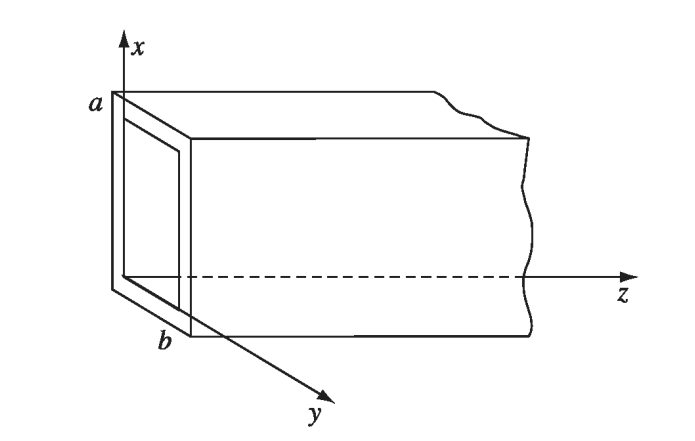
\includegraphics[scale=0.4]{fig/fig-guia-onda-rectangular.png}
\end{center}

\subsubsection{Modos TE:} Analizaremos primero la propagación de modos TE. Entonces debemos encontrar soluciones no-triviales de la ecuación \eqref{EOBzGO} que satisfaga la condición de borde (\ref{CdBGO}b). Usando el método de separación de variables, buscamos soluciones separables de la forma
\begin{equation}
B_z^{0,\rm sep}(x, y) = X(x) Y(y),
\end{equation}
donde las funciones $X(x)$ e $Y(y)$ deben satisfacer
\begin{equation}
\frac{d^2 X}{dx^2} = -k_x^2\,X, \quad \frac{d^2 Y}{dy^2} = -k_y^2\,Y,
\end{equation}
con
\begin{equation}\label{RelDispGOR}
k_x^2 + k_y^2  +k^2 = \frac{\omega^2}{c^2}.
\end{equation} 

La condición de borde en $x=0$ y $x=a$ es $B_x=0$ y la relación \eqref{BxGO} implica entonces que necesariamente $(\partial_xB^0_z)=0$. Esto se traduce en las condiciones $X'(0)=X'(a)=0$. Con esto, las soluciones permitidas son de la forma
\begin{equation}
X(x) \propto \cos(k_x x), \qquad k_x = \frac{m\pi}{a}, \quad m=0,1,2,\dots.
\end{equation}
Similarmente, en los bordes $y=0$ e $y=b$ implican que $(\partial_yB_z)=0$, por lo que las funciones $Y$ deben satisfacer $Y'(0)=Y'(b)=0$. Por lo tanto
\begin{equation}
Y(y) \propto \cos(k_y y), \qquad k_y = \frac{n\pi}{a}, \quad n=0,1,2,\dots.
\end{equation}
Con esto, obtenemos que
\begin{equation}
B^0_z(x, y) = B_0 \cos\left(\frac{m \pi x}{a}\right) \cos\left(\frac{n \pi y}{b}\right).
\end{equation}

Reemplazando en las relaciones \eqref{ExGO}--\eqref{ByGO} obtenemos
\begin{align}
    E^0_x &= \frac{-i\omega}{\omega^2/c^2 - k^2}\left(\frac{n \pi}{b}\right)  B_0\cos\left(\frac{m \pi x}{a}\right) \sin\left(\frac{n \pi y}{b}\right), \label{ExGOTE}\\
    E^0_y &= \frac{i\omega}{\omega^2/c^2 - k^2}\left(\frac{m \pi}{a}\right)  B_0\sin\left(\frac{m \pi x}{a}\right) \cos\left(\frac{n \pi y}{b}\right), \label{EyGOTE}\\
    B^0_x &= -\frac{k}{\omega}E^0_y, \label{BxGOTE}\\
    B^0_y &= \frac{k}{\omega}E^0_x. \label{ByGOTE}
\end{align}
%Podemos ver de aquí que el caso $n=m=0$ no suministra soluciones propagantes, sino 
La relación de dispersión \eqref{RelDispGOR} permite entonces escribir
\begin{equation}\label{kGOR}
k = \sqrt{\frac{\omega^2}{c^2} - \left(\frac{m \pi}{a}\right)^2 - \left(\frac{n \pi}{b}\right)^2}.
\end{equation}
Cada modo TE posible es entonces caracterizado por los valores de $m$ y $n$, y son denotamos como modos TE$_{mn}$. A partir de \eqref{kGOR} vemos que existirá una frecuencia mínima (``cutoff frequency'') $\omega_{mn}$ para cada modo: existirán modos TE propagantes sólo si $\omega>\omega_{mn}$, con
\begin{equation}
\omega_{mn} = c \sqrt{\left(\frac{m \pi}{a}\right)^2 + \left(\frac{n \pi}{b}\right)^2}.
\end{equation}
Si $\omega<\omega_{mn}$ entonces $k$ sería imaginario y no tendríamos una onda propagante, sino un modo que se atenuará exponencialmente.

La solución correspondiente a $m=n=0$ no es un modo propagante, puesto que en este caso $B_z=B_0=\text{cte.}$, $B_x=B_y=0$ y $\vec{E}=\vec{0}$, por lo que en este caso sólo tendremos un campo magnético constate y homogéneo a lo largo de la guía.

 El modo con menor frecuencia de cutoff es el modo TE$_{10}$
\begin{equation}
\omega_{10} = \frac{c \pi}{a},
\end{equation}
que corresponde a una longitud de onda $\lambda_{10}=2\pi c/\omega_{10}=2a$.
Si expresamos \eqref{kGOR} como
\begin{equation}
k = \sqrt{\omega^2 - \omega_{mn}^2},
\end{equation}
entonces podemos escribir la velocidades de fase y grupo de las ondas propagadas como
\begin{equation}
v_{\rm f} = \frac{\omega}{k} = \frac{c}{\sqrt{1 - \left(\frac{\omega_{mn}}{\omega}\right)^2}} > c,
\end{equation}
\begin{equation}
v_{\rm g} = \frac{dk}{d\omega} = c \sqrt{1 - \left(\frac{\omega_{mn}}{\omega}\right)^2} < c.
\end{equation}


El modo TE fundamental, TE$_{10}$
\begin{equation}
E_x=E_z=0, \qquad E_y \propto \sin\left(\frac{\pi x}{a}\right) 
\end{equation}

Podemos reescribir $E_y$ como
\begin{equation}
E_y\propto e^{i(kz+\pi x/a-\omega t)}-e^{i(kz-\pi x/a-\omega t)}.
\end{equation}
Vemos de aquí que este modo puede considerarse como una superposición de dos ondas planas propagándose en diagonal dentro de la guía, con vectores de onda de la forma $\vec{k}_\pm = k\hat{z}\pm(\pi /a)\hat{x}$. El ángulo $\theta$ entre la normal 
\begin{equation}
\cos\theta=\pm\frac{\omega_{nm}}{\omega}
\end{equation}


\subsubsection{Modos TM:}  Si $B_z=0$ entonces buscamos soluciones no triviales para $E_z(x,y)$ que deben satisfacer las condiciones de borde $\vec{E}_z\times\hat{x}=\vec{0}$ en $x=0,a$ y $\vec{E}_z\times\hat{y}=\vec{0}$ en $y=0,b$. Las soluciones separables son entonces de la forma
\begin{equation}
E_z(x, y) = E_0 \sin\left(\frac{m \pi x}{a}\right) \sin\left(\frac{n \pi y}{b}\right)e^{i(kz-\omega t)}, \qquad n,m=1,2,3,\dots.
\end{equation}
La menor frecuencia permitida para los modos TM corresponde al caso en que $n=m=1$, es decir
\begin{equation}
\omega^{\rm TM}_{11}=c\sqrt{\frac{\pi^2}{a^2}+\frac{\pi^2}{b^2}}.
\end{equation}

\subsubsection{Modos TEM:} 

Vemos de \eqref{ExGO}--\eqref{ByGO} que si $E_z=0$ y $B_z=0$ todo el campo se anula, de modo que no existen modos TEM no-triviales en una guía de onda rectangular.

Es posible demostrar que en una guía de ondas completamente hueca, pero de sección transversal arbitratria, no pueden existir modos TEM. En efecto, si $E_z=0$ y $B_z= 0$ entonces la ecuación de Gauss implica que $\partial_xE_x+\partial_yE_y=0$ y la componente $z$ de la ecuación de Faraday implica $\partial_xE_y-\partial_yE_x=0$. Entonces podemos escribir $E_x=-\partial_x\phi$, $E_y=-\partial_y\phi$ con $\nabla^2\phi=0$. Sin embargo, las condiciones de borde (\ref{CdBGO}a) implican que $\phi$ debe ser constante en el borde, y entonces la única solución para $\phi$ es una constante, que implica $E_x=E_y=0$.

\subsection{Guía de onda circular}

Modos TE:
\begin{equation}
B_z^{0,mn}(\rho,\varphi)=B_0J_m(\frac{\beta_{mn}\rho}{R})e^{\pm im\varphi}.
\end{equation}

Modos TM:	
\begin{equation}
E_z^{0,mn}(\rho,\varphi)=E_0J_m(\frac{\alpha_{mn}\rho}{R})e^{\pm im\varphi}.
\end{equation}
Aquí $\alpha_{mn}$ y $\beta_{mn}$ denotan en $n$-ésimo cero de $J_m(x)$ y $J'_m(x)$, respectivamente.

El modo TE$_{11}$ es el que posee la menor frecuencia de corte,
\begin{equation}
\omega_{11}=1.8412\frac{c}{R}.
\end{equation}


\section{Potenciales y transformaciones de gauge}

Las ecuaciones de Maxwell conforman un conjunto de 8 ecuaciones diferenciales
parciales para las 6 componentes del campo electromagnético. A menudo es
\textit{conveniente} reducir el número de variables. Esto puede ser conseguido
expresando los campos en términos de \textbf{potenciales electromagnéticos},
de modo que \textit{las ecuaciones homogéneas de Maxwell sean satisfechas
automáticamente} y el número de campos a determinar se reduce a 4. Estos
potenciales se reducen en los casos estacionarios al conocido potencial
electrostático y al potencial vectorial magnético.

En el caso dinámico general, de (\ref{max2}) podemos concluir que $\vec{B}$
puede ser derivado de un \textbf{potencial vectorial}:
\begin{eqnarray}\label{defA2}
\boxed{\vec{B}=\vec{\nabla}\times \vec{A}.}
\end{eqnarray}
Usando esto en (\ref{max4}), obtenemos:
\begin{equation}
\vec{\nabla}\times \vec{E} = -  \frac{\partial\ }{\partial
t}(\vec{\nabla}\times\vec{A}) = -\vec{\nabla}\times
\frac{\partial\vec{A}}{\partial t},
\end{equation}
es decir,
\begin{eqnarray}
\vec{\nabla}\times \left[ \vec{E} + \frac{\partial \vec{A}}{\partial t} \right]
= \vec{0}.
\end{eqnarray}
De aquí vemos que el campo vectorial dado por la suma $\vec{E} + {\partial
\vec{A}}/{\partial t}$ puede ser escrito como gradiente de un campo escalar, esto es:
\begin{equation}
\vec{E} + \frac{\partial \vec{A}}{\partial t}= - \vec{\nabla}\phi ,
\end{equation}
de donde
\begin{equation}\label{defphi2}
\boxed{\vec{E} =   - \vec{\nabla}\phi - \frac{\partial \vec{A}}{\partial t}.}
\end{equation}
Las ecuaciones (\ref{defA2}) y (\ref{defphi2}) muestran que el campo
electromagnético puede ser escrito en términos de un potencial vectorial
$\vec{A}$ y de un potencial escalar $\phi$. Sin embargo, estas funciones
\textit{no son únicas} para $\vec{E}$ y $\vec{B}$ dados. Es fácil verificar
que el campo electromagnético (y consecuentemente todas las predicciones de la
teoría electromagética) permanece invariante (es decir, con igual valor) bajo las
siguientes transformaciones de los potenciales,
\begin{equation}\marginnote{Transformaciones de gauge}\label{tgg}
\boxed{{\vec{A}}' = \vec{A} - \vec{\nabla}{\chi}, \qquad \phi' =\phi +
\frac{\partial \chi}{\partial t},}
\end{equation}
conocidas como \textbf{transformaciones de gauge} y donde $\chi=\chi(\vec{x},t)$
es una función escalar \textit{arbitraria} del espaciotiempo\footnote{La invariancia
de la teoría electromagnética bajo transformaciones de gauge
desempeña un rol muy importante. La generalización de esta propiedad de
invariancia a \textbf{grupos de simetría interna} permitió formular
teorías consistentes para las \textbf{interacciones débiles} unificadas con la electromagnética (\textbf{electrodébil}) y para la \textbf{interacción fuerte}
(\textit{cromodinámica cuántica}). La \textbf{interacción gravitacional} también puede ser descrita, con algunas peculiaridades, como una \textit{teoría de gauge}.}.

\subsubsection{Ecuaciones de Maxwell inhomogéneas en términos de los
potenciales}
Consideremos el caso de un medio lineal, isótropo y homogéneo. Usando (\ref{defA2}) y (\ref{defphi2}) en las ecuaciones inhomogéneas (\ref{max1}) y (\ref{max3}) encontramos:
\begin{equation}\label{emiap1}
 \nabla^2\phi+\frac{\partial\ }{\partial t}\left(\vec{\nabla}\cdot\vec{A}\right)=-\frac{\rho}{\varepsilon},
\end{equation}
\begin{equation}\label{emiap2}
 \nabla^2\vec{A}-\frac{1}{c^2}\frac{\partial^2\vec{A}}{\partial t^2}-\vec{\nabla}\left(\vec{\nabla}\cdot\vec{A}+\frac{1}{c^2}\frac{\partial\phi }{\partial t}\right)=-\mu\,\vec{J}.
\end{equation}
De esta forma, hemos reducido las ecuaciones de Maxwell a un conjunto de 4 ecuaciones diferenciales parciales para los 4 potenciales. Sin embargo, estas ecuaciones no determinan completamente los potenciales, puesto que las transformaciones de gauge \eqref{tgg} \textit{dejan invariantes} \eqref{emiap1} y \eqref{emiap2}. Esto es natural ya que estas ecuaciones dependen en realidad de los campos eléctrico y magnético, y como vimos las transformaciones de gauge no cambian los valores de estos campos. Además, las ecuaciones \eqref{emiap1} y \eqref{emiap2} están \textit{acopladas}, en el sentido que cada una de estas ecuaciones involucra ambos potenciales electromagnéticos.

Es posible explotar la ``\textbf{libertad de gauge}'' de la electrodinámica (es decir, el hecho que los potenciales no son únicos) para \textit{simplificar algunos cálculos}. Una forma de hacer esto es trabajar con potenciales que satisfagan alguna condición extra o \textbf{gauge}. De hecho, el imponer condiciones extras a los potenciales no sólo es conveniente, sino también \textit{necesario}, ya que las ecuaciones \eqref{emiap1} y \eqref{emiap2} no determinan en forma única los campos $\phi$ y $\vec{A}$. Es posible imponer infinitos gauges diferentes para los potenciales (siempre que sean consistentes con las ecuaciones de Maxwell), pero existen algunos de especial utilidad y popularidad.

\subsubsection{Gauge de Coulomb}
Si el potencial vectorial satisface
\begin{equation}\marginnote{Gauge de Coulomb}\label{gaugeC}
\boxed{ \vec{\nabla}\cdot\vec{A}\stackrel{!}{=}0,}
\end{equation}
se dice que se satisface el \textbf{gauge de Coulomb}, \textbf{gauge de radiación} o \textbf{gauge transversal}. En este caso (\ref{emiap1}) y (\ref{emiap2}) se reducen a
\begin{equation}\label{emiap1GC}
 \nabla^2\phi=-\frac{\rho}{\varepsilon},
\end{equation}
\begin{equation}\label{emiap2GC}
 \nabla^2\vec{A}-\frac{1}{c^2}\frac{\partial^2\vec{A}}{\partial t^2}=-\mu\,\vec{J}+\frac{1}{c^2}\vec{\nabla}\left(\frac{\partial\phi }{\partial t}\right).
\end{equation}

Para probar que \textit{siempre es posible imponer la condición de gauge de Coulomb}, podemos considerar el caso en que inicialmente se trabaje con potenciales $\phi_0$ y $\vec{A}_0$ que no satisfacen la condición (\ref{gaugeC}), es decir, $\vec\nabla\cdot\vec{A}_0\neq 0$, y luego demostrar que es posible realizar una transformación de gauge (\ref{tgg}) con una función $\chi$ tal que los nuevos potenciales sí satisfagan (\ref{gaugeC}). Usando (\ref{tgg}b) requerimos entonces que el nuevo potencial vectorial satisfaga
\begin{equation}
\vec\nabla\cdot\vec{A}=\vec\nabla\cdot(\vec{A}_0-\vec\nabla\chi)\stackrel{!}{=}0.
\end{equation}
Esto implica, como condición necesaria y suficiente, que la función $\chi$ debe satisfacer 
\begin{equation}\label{ePchi}
\nabla^2\chi=\vec\nabla\cdot\vec{A}_0,
\end{equation}
es decir, la ecuación de Poisson con una ``fuente'' conocida ($\vec\nabla\cdot\vec{A}_0$, dados los potenciales originales). Ya que han sido demostrados \textbf{teoremas de existencia} para esta ecuación, es decir, que ella siempre tiene soluciones, queda demostrado que es \textit{posible} imponer el gauge de Coulomb. Note, sin embargo, que la función $\chi$ que determina los nuevos potenciales que satisfacen el gauge de Coulomb \textit{no es única}, ya que si $\chi_1$ es solución de (\ref{ePchi}) entonces $\chi_2=\chi_1+\tilde\chi$ también es solución, siempre que $\tilde\chi$ sea una solución de la ecuación de Laplace ($\nabla^2\tilde\chi=0$). Existe entonces una ``\textbf{libertad remanente}'' para seguir realizando transformaciones de gauge, generadas por funciones $\tilde\chi$ que satisfacen la ecuación de Laplace, y que permiten imponer algunas condiciones\footnote{Ojo: no \textit{cualquier} condición, sino aquellas que sean compatibles con el resto de las condiciones, y con las ecuaciones de Maxwell.} adicionales a los potenciales, siempre dentro de la ``familia de potenciales'' que satisface el gauge de Coulomb.

Una de las conveniencias de este gauge es que \textit{la ecuación (\ref{emiap1GC}) tiene la misma forma que en el caso electrostático}\footnote{Se dice por esto que es ``\textit{coulombiano}'', de ahí uno de los nombres asociados a este gauge.}. Debido a esto, y usando la ``libertad remanente'' mencionada anteriormente, es posible elegir\footnote{!`Pruebe esta afirmación!.} el potencial escalar de la forma siguiente:
\begin{equation}\label{phiGC}
\boxed{ \phi(\vec{x},t)=\frac{1}{4\pi\varepsilon}\int\frac{\rho(\vec{x}',t)}{\left|\vec{x}-\vec{x}'\right|}dV'.}
\end{equation}
Esta solución para el potencial puede entonces ser reemplazada en el lado derecho de \eqref{emiap2GC}. 
%Sin embargo, un cálculo sencillo muestra que este último término cancela la \textit{componente irrotacional} (``longitudinal'') de la corriente. En efecto, asumiendo que las fuentes son localizadas, podemos usar el resultado descrito en el apéndice \ref{Apcamps} y separar la densidad de corriente en una componente longitudinal,  $\vec{J}_{\rm l}$, (o irrotacional, con $\vec\nabla\times\vec{J}_{\rm l}=0$) y una transversal,  $\vec{J}_{\rm t}$, (o solenoidal, con $\vec\nabla\cdot\vec{J}_{\rm t}=0$):
%\begin{equation}
% \vec{J}=\vec{J}_{\rm l}+\vec{J}_{\rm t},
%\end{equation}
%con
%\begin{equation}
% \vec{J}_{\rm l} =-\frac{1}{4\pi}\vec\nabla\int\frac{(\vec\nabla\cdot\vec{J})(\vec{x}')}{|\vec{x}-\vec{x}'|}dV',
%\end{equation}
%\begin{equation}
% \vec{J}_{\rm t} =\frac{1}{4\pi}\vec\nabla\times\int\frac{(\vec\nabla\times\vec{J})(\vec{x}')}{|\vec{x}-\vec{x}'|}dV'.
%\end{equation}
A partir de (\ref{phiGC}), y usando la ecuación de continuidad, podemos escribir el segundo término del lado derecho de \eqref{emiap2GC} sólo en términos de la densidad de corriente, ya que
\begin{eqnarray}
\vec{\nabla}\left(\frac{\partial\phi }{\partial t}\right)&=&  \vec{\nabla}\frac{\partial\ }{\partial t}\left(\frac{1}{4\pi\varepsilon}\int\frac{\rho(\vec{x}',t)}{\left|\vec{x}-\vec{x}'\right|}dV'\right) \\
&=&  \frac{1}{4\pi\varepsilon}\vec{\nabla}\int\frac{\frac{\partial\rho }{\partial t}(\vec{x}',t)}{\left|\vec{x}-\vec{x}'\right|}dV' \\
&=& - \frac{1}{4\pi\varepsilon} \vec{\nabla}\int\frac{(\vec{\nabla}'\cdot\vec{J}')}{\left|\vec{x}-\vec{x}'\right|}dV' .%\\
%&=& \frac{1}{\varepsilon}\vec{J}_{\rm l}.
\end{eqnarray}
Con esto, la ecuación (\ref{emiap2GC}) se reduce a
\begin{equation}\label{emiap3GC}
\boxed{\nabla^2\vec{A}-\frac{1}{c^2}\frac{\partial^2\vec{A}}{\partial t^2}=-\mu\,\vec{J}_{\rm T},}
\end{equation}
donde hemos introducido la \textbf{componente transversal de la densidad de corriente}
\begin{align}
\vec{J}_{\rm T} &:= \vec{J}-\frac{1}{c^2\mu}\vec{\nabla}\left(\frac{\partial\phi }{\partial t}\right) \\
&= \vec{J}+\frac{1}{4\pi} \vec{\nabla}\int\frac{(\vec{\nabla}'\cdot\vec{J}')}{\left|\vec{x}-\vec{x}'\right|}dV'.
\end{align}
Se dice que este campo es \textit{transversal} porque satisface
\begin{equation}
\vec\nabla\cdot\vec{J}_{\rm T}\equiv 0.
\end{equation}

En resumen, \textit{en el gauge de Coulomb el potencial vectorial satisface la  \textit{ecuación de onda inhomogénea}, con un término fuente determinado sólo por la componente transversal de la densidad de corriente}. Además, en este gauge  sólo el potencial vectorial contribuye a los \textbf{campos radiativos}\footnote{Como veremos en el capítulo \ref{caprad}, se dice que un campo electromagnético es radiativo si su contribución a la energía radiada muy lejos de las fuentes (``en el infinito'') es no nula.}. En cambio, el potencial escalar \eqref{phiGC} es no-radiativo como consecuencia de que su valor decae al menos tan rápido como $1/r$ a grandes distancias de la fuente.

El gauge de Coulomb es a menudo usado en regiones donde no hay fuentes presentes. En este caso es posible elegir $\phi=0$, ver \eqref{phiGC}, de modo que toda la información del campo electromagnético está contenida en el potencial vectorial $\vec{A}$.


\subsubsection{Gauge de Lorenz}
Otro gauge común es el \textbf{gauge de Lorenz}\footnote{Nombrado en recuerdo de Ludvig Valentin Lorenz (1829-1891): Matemático y Físico Danés. Ver \url{http://es.wikipedia.org/wiki/Ludvig_Lorenz}, quien consideró esta elección en 1867.}, que usualmente es escrito como
\begin{equation}\marginnote{Gauge de Lorenz}\label{gLorenz}
\boxed{\frac{1}{c^2}\frac{\partial\phi}{\partial t}+\vec{\nabla}\cdot\vec{A}\stackrel{!}{=}0,}
\end{equation}
y que \textit{permite desacoplar las ecuaciones} (\ref{emiap1}) y (\ref{emiap2}).
En efecto, si (\ref{gLorenz}) es satisfecha entonces (\ref{emiap1}) y (\ref{emiap2}) se reducen a
\begin{equation}\label{emiap1gL}
 \nabla^2\phi-\frac{1}{c^2}\frac{\partial^2\phi}{\partial t^2}=-\frac{\rho}{\varepsilon},
\end{equation}
\begin{equation}\label{emiap2gL}
 \nabla^2\vec{A}-\frac{1}{c^2}\frac{\partial^2\vec{A}}{\partial t^2}=-\mu\,\vec{J},
\end{equation}
o, introduciendo el \textbf{operador de onda} (u operador de  d'\,Alembert\footnote{Jean Le Rond d'\,Alembert (1717-1783): matemático, filósofo y enciclopedista francés. Ver \url{http://es.wikipedia.org/wiki/Jean_le_Rond_d\%27Alembert}.}), 
$\Box:= c^{-2}{\partial^2}/{\partial t^2}-\nabla^2$,
\begin{equation}\label{emiap1gL2}
 \Box\phi=\frac{\rho}{\varepsilon},
\end{equation}
\begin{equation}\label{emiap2gL2}
 \Box\vec{A}=\mu\,\vec{J}.
\end{equation}

Análogamente al caso del gauge de Coulomb, puede probarse que \textit{el gauge de Lorenz siempre puede ser impuesto}, considerando que inicialmente se usen potenciales ($\phi_0$ y $\vec{A}_0$) que no lo satisfacen, y mostrando que puede encontrarse una función $\chi$ que genere la transformación de gauge apropiada para que los nuevos potenciales sí la satisfagan. En este caso, la condición sobre la función $\chi$ requerida es que
\begin{eqnarray}
0&\stackrel{!}{=}&\frac{1}{c^2}\frac{\partial\phi}{\partial t}+\vec{\nabla}\cdot\vec{A} \\
&=&\frac{1}{c^2}\frac{\partial\ }{\partial t}\left(\phi_0+\frac{\partial\chi}{\partial t}\right)+\vec{\nabla}\cdot\left(\vec{A}_0-\vec\nabla\chi\right) \\
&=&\left(\frac{1}{c^2}\frac{\partial\phi_0}{\partial t} +\vec{\nabla}\cdot\vec{A}_0\right) +\frac{1}{c^2}\frac{\partial^2\chi }{\partial t^2}-\nabla^2\chi,
\end{eqnarray}
es decir, que satisfaga la ecuación de onda inhomogénea:
\begin{equation}
\Box\chi=-\left(\frac{1}{c^2}\frac{\partial\phi_0}{\partial t} +\vec{\nabla}\cdot\vec{A}_0\right).
\end{equation}
La existencia de soluciones de esta ecuación está garantizada. Análogamente al caso del gauge de Coulomb, la función buscada no es única, sino que existe una libertad remanente para realizar transformaciones de gauge ``dentro del gauge de Lorenz'', generadas por funciones $\tilde\chi$ que satisfagan la ecuación de onda, $\Box\tilde\chi=0$. 

El gauge de Lorenz es usado comúnmente en el contexto de la teoría de Especial de la Relatividad, ya que en el vacío (cuando $\varepsilon=\varepsilon_0$ y $\mu=\mu_0$ y por lo tanto $c=c_0$) la condición (\ref{gLorenz}) así como (\ref{emiap1gL2}) y (\ref{emiap2gL2}), \textit{mantienen su forma inalterada en cualquier sistema de referencia inercial} (son \textit{covariantes} bajo transformaciones de Lorentz). Esto tiene como consecuencia que toda expresión que involucre a los potenciales electromagéticos (que satisfagan el gauge de Lorenz) tendrá la \textit{misma forma en todo Sistema de Referencia Inercial}. Esto no ocurre, por ejemplo, si se usan potenciales que satisfagan el gauge de Coulomb.

\newpage
\chapter{Teoría Clásica de la Radiación Electromagnética}\label{caprad}

\section{Resolviendo las ecuaciones de Maxwell.}\label{resolvmax}

Las ecuaciones de Maxwell inhomogéneas, escritas en términos de los potenciales electromagnéticos y en el gauge de Lorenz, se reducen a
%\begin{equation}
%\boxed{\Box A^\mu   =\frac{4\pi}{c}J^\mu ,}
%\end{equation}
%o, equivalentemente,
%\begin{equation}
%\Box \phi   =4\pi \rho, \qquad \Box \vec{A}=\frac{4\pi}{c}\vec{J}.
%\end{equation}
\begin{equation}
 \Box\phi=\frac{\rho}{\varepsilon}, \qquad  \Box\vec{A}=\mu\,\vec{J}.
\end{equation}
Estas son las ecuaciones que resolveremos: las ecuaciones de onda
inhomogéneas para fuentes dadas. Todas ellas son de la forma
\begin{equation}
\Box \Psi(\vec{x},t)=g(\vec{x},t), \label{oih}
\end{equation}
con una función ``fuente'' $g(\vec{x},t)$ dada.


\subsection{Ecuación de Helmholtz inhomogénea y función de Green independiente del tiempo}
\subsubsection{Transformada de Fourier}
Primero introduciremos la \textbf{transformada de Fourier temporal} de los campos involucrados (suponemos que estos campos son cuadrado-integrables),
\begin{equation}
\bar{\Psi}(\vec{x},\omega):=\frac{1}{\sqrt{2\pi}}\int_{-\infty}^\infty
\Psi(\vec{x},t)e^{-i\omega t}\,dt,
\end{equation}
\begin{equation}
\bar{g}(\vec{x},\omega):=\frac{1}{\sqrt{2\pi}}\int_{-\infty}^\infty
g(\vec{x},t)e^{-i\omega t}\,dt ,
\end{equation}
y entonces
\begin{equation}
g(\vec{x},t)=\frac{1}{\sqrt{2\pi}}\int_{-\infty}^\infty
\bar{g}(\vec{x},\omega)e^{+i\omega t}\,d\omega,
\end{equation}
\begin{equation}
\Psi(\vec{x},t)=\frac{1}{\sqrt{2\pi}}\int_{-\infty}^\infty
\bar{\Psi}(\vec{x},\omega)e^{+i\omega t}\,d\omega.
\end{equation}

Usando estas transformaciones la ecuación (\ref{oih}) se reduce a la ecuación de
Helmholtz inhomogénea:
\begin{equation}
\left[ \nabla^2+k^2\right] \bar{\Psi}(\vec{x},\omega)=-\bar{g}(\vec{x},\omega),
\label{Hih}
\end{equation}
con $k:=\omega/c$. Resolveremos esta ecuación \textit{independiente del tiempo} por medio del método de la función de Green.

\subsubsection{Función de Green independiente del tiempo}
La función de Green asociada a nuestro problema es
\begin{equation}
\left[ \nabla^2+k^2\right] G(\vec{x},\vec{x}')=+\delta^{(3)}(\vec{x}-\vec{x}').
\label{ecGreen}
\end{equation}
Si logramos resolver (\ref{ecGreen}) y encontrar una solución $G(\vec{x},\vec{x}')$ entonces una solución particular de (\ref{Hih}) es de la forma
\begin{equation}
\bar{\Psi}(\vec{x},\omega)=-\int G(\vec{x},\vec{x}')\bar{g}(\vec{x}',\omega)\,dV'.
\end{equation}
La función de Green $G(\vec{x},\vec{x}')$ puede considerarse como un caso particular de solución de (\ref{Hih}) correspondiente a una función fuente $\bar{g}=\delta^{(3)}(\vec{x}-\vec{x}')$. En términos más físicos, la función de Green $G(\vec{x},\vec{x}')$ es proporcional al campo producido por una \textbf{fuente puntual}. En efecto, si $g(\vec{x},t)=f(t)\delta^{(3)}(\vec{x}-\vec{x}')$, entonces $\bar{g}(\vec{x},\omega)=\bar{f}(\omega)\delta^{(3)}(\vec{x}-\vec{x}')$, donde $\bar{f}(\omega)$ es la transformada de Fourier de $f(t)$. De lo anterior, vemos que en este caso la solución de (\ref{Hih}) es de la forma $-\bar{f}(\omega)G(\vec{x},\vec{x}')$.

La función de Green que satisface (\ref{ecGreen}) \textit{no es única}, siempre es posible sumar una solución de la ecuación de Helmholtz homogénea. De entre las posibles soluciones, encontraremos aquella que satisfaga \textit{condiciones de simetría apropiadas a nuestro problema}. En particular, deseamos encontrar las soluciones particulares que describan los campos \textit{generados por una distribución de cargas y corrientes dada}, sin incluir los campos generados por \textit{fuentes externas al sistema} (y que satisfacen la ecuación homogénea en el dominio bajo consideración).

Ya que $G(\vec{x},\vec{x}')$ determina la dependencia espacial de la solución correspondiente a una carga puntual situada en $\vec{x}'$, esperamos que ésta sea esféricamente simétrica en torno a este punto (``isotropía del espacio''), y sólo dependiente de la diferencia entre $\vec{x}$ y $\vec{x}'$ (``homogeneidad del espacio''). Entonces, supondremos que $G$ depende de $\vec{x}$ y $\vec{x}'$ sólo a través de la combinación $|\vec{x}-\vec{x}'|$. Si
\begin{equation}
G(\vec{x},\vec{x}')\stackrel{!}{=}G(|\vec{x}-\vec{x}'|),
\end{equation}
 la ecuación (\ref{ecGreen}) se reduce a
\begin{equation}
\left[ \nabla^2+k^2\right] G(r)=\delta^{(3)}(\vec{r}), \qquad r:=|\vec{r}|.
\end{equation}
%ya que, sin perder generalidad, es posible elegir $\vec{x}'=\vec{0}$.
En coordenadas esféricas, tendremos entonces que
\begin{equation}
 \frac{1}{r^2}\frac{d}{dr}\left( r^2\frac{dG}{dr}\right) +k^2G(r)=\delta^{(3)}(\vec{r})
.\label{HelmG}
\end{equation}
Es directo resolver (\ref{HelmG}) para puntos $r\neq 0$. Obtenemos:
\begin{equation}
G(r)=\alpha\frac{e^{\pm ikr}}{r}, \label{G0}
\end{equation}
para $r\neq 0$. La constante $\alpha$ debe ser determinada de modo que
(\ref{G0}) sea válida para todo punto, incluyendo el punto $r=0$. Usando
$\vec{\nabla}r=-r^2\vec{\nabla}\left({1}/{r}\right) $, podemos escribir:
\begin{eqnarray}
\vec{\nabla}G&=&\pm ik\alpha\frac{1}{r}\left( \vec{\nabla}r\right) e^{\pm
ikr}+\alpha e^{\pm ikr} \vec{\nabla}\left( \frac{1}{r}\right) \\
&=&\mp ik\alpha r\vec{\nabla}\left( \frac{1}{r}\right)  e^{\pm ikr}+\alpha
e^{\pm ikr} \vec{\nabla}\left( \frac{1}{r}\right) .
\end{eqnarray}
Similarmente,
\begin{eqnarray}
\nabla^2G&=&\vec{\nabla}\cdot \vec{\nabla}G \\
&=&\mp ik\alpha \left( \vec{\nabla}r\right)\cdot\vec{\nabla}\left(
\frac{1}{r}\right)  e^{\pm ikr}\mp ik\alpha r \nabla^2\left( \frac{1}{r}\right)
e^{\pm ikr}+k^2\alpha r\left( \vec{\nabla}r\right)\cdot\vec{\nabla}\left(
\frac{1}{r}\right)  e^{\pm ikr}\nonumber\\
&&\pm ik\alpha e^{\pm ikr} \left( \vec{\nabla}r\right)\cdot\vec{\nabla}\left(
\frac{1}{r}\right) +\alpha e^{\pm ikr}\nabla^2\left( \frac{1}{r}\right) \\
&=&\mp ik\alpha r \nabla^2\left( \frac{1}{r}\right)  e^{\pm ikr}+k^2\alpha
r\left( \vec{\nabla}r\right)\cdot\vec{\nabla}\left( \frac{1}{r}\right)  e^{\pm
ikr}+\alpha e^{\pm ikr}\nabla^2\left( \frac{1}{r}\right) \\
&=&\mp ik\alpha r \nabla^2\left( \frac{1}{r}\right)  e^{\pm ikr}-k^2\alpha
\frac{1}{r} \left|\vec{\nabla}r\right|^2  e^{\pm ikr}+\alpha e^{\pm
ikr}\nabla^2\left( \frac{1}{r}\right).
\end{eqnarray}
Usando ahora $\nabla^2\left({1}/{r}\right) =-4\pi\delta^{(3)}(\vec{r})$,
$f(r)\delta^{(3)}(\vec{r})=f(0)\delta^{(3)}(\vec{r})$ para una función $f(r)$ arbitraria, y
$\vec{\nabla}r=\hat{r}$, de modo que $|\vec{\nabla}r|=1$,
encontramos
\begin{eqnarray}
\nabla^2G&=&\pm 4\pi ik\alpha r  e^{\pm ikr}\delta^{(3)}(\vec{r}) -k^2\alpha \frac{1}{r}
e^{\pm ikr}-4\pi\alpha e^{\pm ikr}\delta^{(3)}(\vec{r}) \\
&=&0-k^2\alpha \frac{e^{\pm ikr}}{r}   -4\pi\alpha \delta^{(3)}(\vec{r}) \\
&=&-k^2G(r) -4\pi\alpha \delta^{(3)}(\vec{r}) .\label{lapG}
\end{eqnarray}
Comparando (\ref{lapG}) con (\ref{HelmG}) obtenemos $\alpha=-{1}/{4\pi}$, de
modo que la función de Green para nuestro problema es
\begin{equation}
\boxed{G(\vec{x},\vec{x}')=-\frac{1}{4\pi}\frac{e^{\pm
ik|\vec{x}-\vec{x}'|}}{|\vec{x}-\vec{x}'|}, \qquad k:=\frac{\omega}{c}.} \label{GreenH}
\end{equation}


\subsection{Potenciales retardados}
Con la función de Green (\ref{GreenH}) obtenemos la solución particular para la
transformada de Fourier $\bar{\Psi}(\vec{x},\omega)$:
\begin{equation}
\bar{\Psi}(\vec{x},\omega)=\frac{1}{4\pi}\int
\bar{g}(\vec{x}',\omega)\frac{e^{\pm
ik|\vec{x}-\vec{x}'|}}{|\vec{x}-\vec{x}'|}\,dV' .
\end{equation}
Con esto, podemos finalmente calcular la solución particular de la ecuación de
onda inhomogénea (\ref{oih}):
\begin{eqnarray}
\Psi(\vec{x},t)&=&\frac{1}{\sqrt{2\pi}}\frac{1}{4\pi}\int_{V'}\int_{-\infty}
^\infty \bar{g}(\vec{x}',\omega)\frac{e^{\pm
ik|\vec{x}-\vec{x}'|}}{|\vec{x}-\vec{x}'|}e^{i\omega t}\,d\omega\,dV'  \\
&=&\frac{1}{\sqrt{2\pi}}\frac{1}{4\pi}\int_{V'}\frac{1}{|\vec{x}-\vec{x}'|}\int_
{-\infty}^\infty \bar{g}(\vec{x}',\omega)e^{i\omega t_{\pm}}\,d\omega \,dV' \\
&=&\frac{1}{4\pi}\int_{V'} \frac{g(\vec{x}',t_{\pm})}{|\vec{x}-\vec{x}'|}\,dV' .
\end{eqnarray}
En la expresión anterior hemos denotado
\begin{equation}
t_{\pm}(\vec{x},\vec{x}',t):=t\pm \frac{|\vec{x}-\vec{x}'|}{c}.
\end{equation}
Los \textbf{potenciales retardados} corresponden a la solución con
\begin{equation}
\boxed{t_{\rm ret}(\vec{x},\vec{x}',t):=t-\frac{|\vec{x}-\vec{x}'|}{c},} \label{deftret}
\end{equation}
que es llamado el \textbf{tiempo retardado} (puesto que $t_{\rm ret}\le t$), de modo que
\begin{equation}
\boxed{\phi_{\rm ret}(\vec{x},t)=\frac{1}{4\pi\varepsilon}\int_{V'}
\frac{\rho(\vec{x}',t_{\rm ret})}{|\vec{x}-\vec{x}'|}\,dV',} \qquad \boxed{\vec{A}_{\rm
ret}(\vec{x},t)=\frac{\mu}{4\pi}\int_{V'}
\frac{\vec{J}(\vec{x}',t_{\rm ret})}{|\vec{x}-\vec{x}'|}\,dV' ,} \label{potret}
\end{equation}
suministran expresiones para los potenciales electromagnéticos en un punto
$\vec{x}$ y en un instante $t$ dado \textit{en términos de la distribución de cargas y corrientes en tiempos anteriores a} $t$ (``solución causal''). En otras palabras, los potenciales (\ref{potret}) permiten \textit{pre}decir los campos producidos por un sistema de cargas dado. Por otro lado, la solución correspondiente al \textbf{tiempo avanzado} $t_{\rm av}:=t+{|\vec{x}-\vec{x}'|}/{c}\ge t$ relaciona los campos, en cada instante $t$, con la distribución de cargas en \textit{tiempos posteriores a }$t$ (``solución acausal'').

Considere por simplicidad el caso en que las fuentes del sistema ($\vec{\rho}$ y $\vec{J}$) son no nulas sólo en un intervalo finito de tiempo $t\in (t_{\rm i},t_{\rm f})$. Esto ocurre, por ejemplo, en un condensador inicialmente descargado, que luego se carga al ser conectado a una batería, y que luego se descarga. Si $\Psi_{\rm i}(\vec{x},t)$ es la solución del campo en tiempos $t<t_{\rm i}$ entonces podemos usar los potenciales retardados para \textit{pre}decir el campo en tiempos posteriores: $\Psi=\Psi_{\rm i}+\Psi_{\rm ret}$, ya que $\Psi_{\rm ret}(\vec{x},t)=0$ para $t<t_{\rm i}$. Por el contrario, si la información de la que disponemos es el campo $\Psi_{\rm f}$ en tiempos posteriores $t>t_{\rm f}$ entonces podemos usar los potenciales avanzados para ``\textit{retro}decir" los valores anteriores del campo: $\Psi=\Psi_{\rm f}+\Psi_{\rm av}$, ya que 
$\Psi_{\rm ret}(\vec{x},t)=0$ para $t>t_{\rm f}$.

Las expresiones para los potenciales retardados son similares a aquellas válidas los casos electrostático y magnetostático, ver \eqref{perho} y \eqref{defA} respectivamente, salvo que las fuentes dentro de la integral están evaluadas en el tiempo retardado, que depende tanto del tiempo como de la posición\footnote{Esta propiedad no es en general válida si los potenciales satisfacen gauges distintos al de Lorenz.}. Esta solución muestra que los campos en un punto $\vec{x}$ y tiempo $t$ dado son una  \textit{superposición de términos proporcionales a las fuentes ubicadas en \textit{cada punto} $\vec{x}'$, pero en tiempos anteriores} $t_{\rm ret}$, de forma tal que el \textit{evento}\footnote{es decir, un punto determinado del espacio y del tiempo.} definido por $(ct_{\rm ret},\vec{x}')$ tiene una \textit{relación tipo luz} con el evento $(ct,\vec{x})$. Esto último significa, como se desprende de (\ref{deftret}), que
\begin{equation}\marginnote{relación tipo luz}
 c^2(t-t_{\rm ret})^2-|\vec{x}-\vec{x}'|^2=0.
\end{equation}
En otras palabras, los valores del campo en un evento dado están determinados por los valores de las fuentes en los puntos del \textbf{cono de luz pasado} asociado a tal evento. Ver figura \ref{fig:cdl2}.
\begin{figure}[!h]
\centerline{\includegraphics[height=5.5cm]{fig/fig-cono-de-luz-01.pdf}}
\caption{Cono de luz}
\label{fig:cdl2}
\end{figure}

Otra consecuencia directa es que cualquier \textit{cambio} en la configuración de las fuentes en un punto afectará a los campos en otro punto sólo en tiempos posteriores, luego de un intervalo de tiempo igual al tiempo de vuelo de una señal luminosa que los conecte. En otras palabras: \textit{los cambios de los campos producidos por cambios de las fuentes se propagan con rapidez $c=1/\sqrt{\varepsilon\mu}$}. Equivalentemente, el valor de las fuentes en un determinado evento contribuye a los valores de los campos sólo en eventos situados sobre el \textit{cono de luz futuro} del evento fuente.


\section{Ecuaciones de Jefimenko}
A partir de las expresiones para los potenciales retardados en el gauge de Lorenz, es decir las ecuaciones \eqref{potret}, podemos calcular los campos eléctrico y magnético producidos por una distribución (arbitraria, pero compacta) de cargas y corrientes:
\begin{equation}
\vec{E}(\vec{x},t)=\frac{1}{4\pi\varepsilon}\int_V \left[  \frac{\rho(\vec{x}',t_{\rm ret})(\vec{x}-\vec{x}')}{\vert \vec{x}-\vec{x}' \vert^3} + \frac{1}{c}\frac{ \dot\rho(\vec{x}',t_{\rm ret})(\vec{x}-\vec{x}')}{\vert\vec{x}-\vec{x}'\vert^2} -\frac{1}{c^2}\frac{\dot{\vec{J}} (\vec{x}',t_{\rm ret})}{\vert\vec{x}-\vec{x}' \vert} \right] dV',
\end{equation}
\begin{equation}
\vec{B}(\vec{x},t)=\frac{\mu}{4\pi} \int_V\left[
\frac{\vec{J}(\vec{x}',t_{\rm ret})\times(\vec{x}-\vec{x}')}{\vert \vec{x}-\vec{x}'\vert^3}+ \frac{1}{c}\frac{ \dot{\vec{J}}(\vec{x}',t_{\rm ret})\times(\vec{x}-\vec{x}')}{\vert\vec{x}-\vec{x}' \vert^2} \right]dV', \label{b3}
\end{equation}
donde $\dot{f}(\vec{x},t)$ denota la derivada partial respecto a la variable temporal de la que depende la función $f(\vec{x},t)$, es decir $\dot{f}(\vec{x},t):=(\partial_t f)(\vec{x},t)$. Las relaciones anteriores son conocidas como \textbf{ecuaciones de Jefimenko}\footnote{\href{http://en.wikipedia.org/wiki/Jefimenko}{Oleg Jefimenko} (1922-2009): físico estadounidense.}. Note que estas expresiones para los campos eléctrico y magnético difieren de aquellas que se encontrarían directamente la solución de las ecuaciones inhomogéneas \eqref{EcOihE} y \eqref{EcOihB}. ?`Puede explicar por qué ocurre esto?.


\section{Potenciales de Liénard-Wiechert}

Se conoce como \textbf{potenciales de Liénard}\footnote{\href{https://en.wikipedia.org/wiki/Alfred-Marie_Li\%C3\%A9nard}{Alfred Marie Liénard} (1869-1958): físico francés.}\textbf{-Wiechert}\footnote{\href{https://en.wikipedia.org/wiki/Emil_Wiechert}{Johann Emil Wiechert} (1861-1928): (geo)físico alemán.} a los potenciales retardados generados por una \textit{carga puntual} $q$ \textit{que se mueve en forma conocida, pero arbitraria}. Denotaremos la trayectoria de la carga usando la función $\vec{z}(t)$. Ver figura (\ref{fig:LW}).
\begin{figure}[ht]
\centerline{\includegraphics[height=5.5cm]{fig/fig-cono-de-luz-02.pdf}}
\caption{Trayectoria de una carga puntual y cono de luz asociado al evento $(ct,\vec{x})$.}
\label{fig:LW}
\end{figure}
En este caso, la densidad de carga y de corriente están dadas por
\begin{equation}
\rho(\vec{x},t)=q\delta^{(3)}(\vec{x}-\vec{z}(t)), \qquad
\vec{J}(\vec{x},t)=q\vec{v}(t)\delta^{(3)}(\vec{x}-\vec{z}(t)),
\end{equation}
donde $\vec{v}(t)={d\vec{z}}/{dt}$ es la velocidad instantánea de la carga. Por lo tanto, los potenciales retardados (\ref{potret}) se reducen a
\begin{equation}
\phi_{\rm ret}(\vec{x},t)=\frac{q}{4\pi\varepsilon}\int_{V'}
\frac{\delta^{(3)}(\vec{x}'-\vec{z}(t_{\rm ret}))}{|\vec{x}-\vec{x}'|}\,dV', \quad
\vec{A}_{\rm ret}(\vec{x},t)=\frac{q\mu}{4\pi}\int_{V'}
\frac{\vec{v}(t_{\rm ret})\delta^{(3)}(\vec{x}'-\vec{z}(t_{\rm ret}))}{|\vec{x}-\vec{x}'|}\,dV'  \label{potretq1}
\end{equation}
o, más explícitamente,
\begin{equation}
\phi_{\rm ret}(\vec{x},t)=\frac{q}{4\pi\varepsilon}\int_{V'}
\frac{\delta^{(3)}(\vec{x}'-\vec{z}(t-|\vec{x}-\vec{x}'|/c))}{|\vec{x}-\vec{x}'|}\,dV', \end{equation}
\begin{equation}
\vec{A}_{\rm ret}(\vec{x},t)=\frac{q\mu}{4\pi}\int_{V'}
\frac{\vec{v}(t-|\vec{x}-\vec{x}'|/c)\,\delta^{(3)}(\vec{x}'-\vec{z}(t-|\vec{x}-\vec{x}'|/c))}{|\vec{x}-\vec{x}'|}\,dV' . \label{potretq2}
\end{equation}
Ambas expresiones son de la forma
\begin{equation}
I(\vec{x},t)=\int_{V'}
f(\vec{x},\vec{x}',t)\,\delta^{(3)}(\vec{x}'-\vec{z}(t-|\vec{x}-\vec{x}'|/c))\,d^3x' . \label{potretqg1}
\end{equation}

Para calcular este tipo de integrales, expresaremos la delta de Dirac 3-dimensional como una integral sobre la variable (temporal) auxiliar $T$:
\begin{equation}
 \delta^{(3)}(\vec{x}'-\vec{z}(t-|\vec{x}-\vec{x}'|/c))=\int_{-\infty}^\infty \delta^{(3)}(\vec{x}'-\vec{z}(T))\,\delta(T-t+|\vec{x}-\vec{x}'|/c)\, dT.
\end{equation}
Con esto,
\begin{equation}
I(\vec{x},t)=\int_{T}\int_{V'}
f(\vec{x},\vec{x}',t)\,\delta^{(3)}(\vec{x}'-\vec{z}(T))\,\delta(T-t+|\vec{x}-\vec{x}'|/c)\,d^3x' \, dT. \label{potretqgm11}
\end{equation}
Expresada de esta forma, es sencillo realizar la integral espacial, puesto que la delta de Dirac 3-dimensional evaluará la coordenada $\vec{x}'$ en el punto $\vec{z}(T)$, es decir, en un punto sobre la trayectoria de la carga. Así, obtenemos
\begin{equation}
I(\vec{x},t)=\int_{-\infty}^\infty f(\vec{x},\vec{z}(T),t)\,\delta(T-t+|\vec{x}-\vec{z}(T)|/c)\, dT. \label{potretqgm12}
\end{equation}
El argumento de la delta de Dirac es una función no trivial $g$ de la variable auxiliar $T$. Denotamos
\begin{equation}
 g(T):=T-t+\frac{1}{c}|\vec{x}-\vec{z}(T)|,
\end{equation}
de modo que
\begin{eqnarray}
I(\vec{x},t)&=&\int_{-\infty}^\infty f(\vec{x},\vec{z}(T),t)\,\delta(g(T))\, dT \\
&=&\int_{-\infty}^\infty f(\vec{x},\vec{z}(T),t)\frac{\delta(T-t')}{|g'(t')|}\, dT \\
&=&\frac{f(\vec{x},\vec{z}(t'),t)}{|g'(t')|}, \label{Ir}
\end{eqnarray}
donde $g'$ es la función derivada de $g$ y $t'$ es la solución de la ecuación $g(t')=0$, es decir, de
\begin{equation}
 t'=t-\frac{1}{c}|\vec{x}-\vec{z}(t')|. \label{t'}
\end{equation}
Esta relación define una \textit{ecuación algebraica} para $t'$ cuya solución define, \textit{conocida la trayectoria de la carga}, un tiempo retardado particular $t'=t'(\vec{x},t)$ para cada valor de $\vec{x}$ y $t$. 

Usando la regla de la cadena, encontramos
\begin{equation}
 g'(t')=1-\frac{1}{c}\frac{\vec{v}(t')\cdot\left(\vec{x}-\vec{z}(t')\right)}{\left|\vec{x}-\vec{z}(t')\right|}=1-\vec{\beta}(t')\cdot\hat{n}(t')>0 \label{gp},
\end{equation}
para $|\vec\beta|<1$, con $\vec\beta:=\vec{v}/c$. Por ahora, supondremos que siempre la velocidad de la partícula es menor que la velocidad de la luz en el medio. Entonces, reemplazando (\ref{gp}) en (\ref{Ir}), se encuentra que
\begin{equation}
 I(\vec{x},t)=\frac{f(\vec{x},\vec{z}(t'),t)}{1-\vec{\beta}(t')\cdot\hat{n}(t')}. \label{Ir2}
\end{equation}
Para el caso del potencial, encontramos así que
\begin{equation}
\phi_{\rm ret}(\vec{x},t)=\frac{1}{4\pi\varepsilon}\frac{q}{\left|\vec{x}-\vec{z}(t')\right|}\frac{1}{\left( 1-\vec\beta(t')\cdot\hat{n}(t')\right) }.
 \end{equation}
Análogamente, en el caso del potencial vectorial, obtenemos
\begin{equation}
\vec{A}_{\rm ret}(\vec{x},t)=\frac{\mu c}{4\pi}\frac{q}{\left|\vec{x}-\vec{z}(t')\right|}
\frac{\vec{\beta}(t')}{\left( 1-\vec\beta(t')\cdot\hat{n}(t')\right) }.
 \end{equation}
 
Debe recordarse que en estas expresiones $t'$ es una función de $\vec{x}$ y $t$, determinada por la solución de (\ref{t'}) para una trayectoria dada. La condición (\ref{t'}) implica que el evento donde se quiere determinar el campo, con coordenadas $(ct,\vec{x})$, y el evento sobre la trayectoria de la carga en el tiempo $t'$, con coordenadas $(ct',\vec{z}(t'))$, tienen una \textit{relación tipo luz}, ya que
\begin{equation}
 c^2(t-t')^2-|\vec{x}-\vec{z}(t')|^2=0.
\end{equation}

En otras palabras, el evento con coordenadas $(ct',\vec{z}(t'))$ es la \textit{intersección entre el cono de luz pasado asociado a $(ct,\vec{x})$ y la línea de mundo de la carga}. Ver figura \ref{fig:LW}. Los potenciales en un evento $(ct,\vec{x})$ dado dependen entonces sólo de las propiedades de la carga (posición y velocidad) en el tiempo retardado $t'(\vec{x},t)$.

Usualmente, se simplifica la notación definiendo
\begin{equation}
 \vec{R}:=\vec{x}-\vec{z}(t'), \qquad R:=\left|\vec{x}-\vec{z}(t')\right|, \qquad \hat{n}:=\frac{\vec{R}}{R}, \label{defR}
\end{equation}
y denotando la evaluación de todas las funciones dependientes del tiempo en $t'$ por $f(t'):=\left.f\right|_{\rm ret}$, de modo que
\begin{equation}
\boxed{\phi_{\rm ret}(\vec{x},t)=\frac{1}{4\pi\varepsilon}\left. \frac{q}{ R\left(
1-\vec{\beta}\cdot\hat{n}\right) }\right|_{\rm ret}, } \qquad
\boxed{\vec{A}_{\rm ret}(\vec{x},t)=\frac{\mu c}{4\pi}\left. \frac{q\vec{\beta}}{ R\left(1-\vec{\beta}\cdot\hat{n}\right) }\right|_{\rm ret}.} \label{potretq}
\end{equation}

Note que en este caso los potenciales retardados están relacionados por
\begin{equation}
\vec{A}_{\rm ret}(\vec{x},t)=\frac{1}{c}\phi_{\rm ret}(\vec{x},t)\left.\vec{\beta}\right|_{\rm ret}.
\end{equation}


\subsection{Derivación alternativa*}
Podemos integrar (\ref{potretqg1}) cambiando de variable de integración de $\vec{x}'$ a la nueva variable $\vec{y}$, definida por (recuérdese que, para efectos de la integración, $t$ es un parámetro y $\vec{z}$ una función conocida)
\begin{equation}
 \vec{y}(\vec{x'}):=\vec{x}'-\vec{z}(t-|\vec{x}-\vec{x}'|/c). \label{txy}
\end{equation}
En términos de $\vec{y}$ la integral (\ref{potretqg1}) adopta la forma
\begin{equation}
I(\vec{x},t)=\int f(\vec{x},\vec{x}'(\vec{y}),t)\delta^{(3)}(\vec{y})
\left|\frac{\partial \vec{x}}{\partial \vec{y}}\right|\,d^3y, \label{potretqg2}
\end{equation}
donde $\left|\frac{\partial \vec{x}'}{\partial \vec{y}}\right|=\left|\frac{\partial \vec{y}}{\partial \vec{x}'}\right|^{-1}$ es el jacobiano de la transformación. A partir de (\ref{txy}) encontramos que
\begin{eqnarray}
\frac{\partial y^i}{\partial x'^j}&=&\delta^i_j-\dot{z}^i(t_{\rm ret})\frac{\partial t_{\rm ret}}{\partial x'^j} \\
&=&\delta^i_j+\frac{1}{c}v^i(t_{\rm ret})\partial'_j|\vec{x}-\vec{x}'|\\
&=&\delta^i_j-\beta^i(t_{\rm ret})\frac{(x^j-x'^j)}{|\vec{x}-\vec{x}'|}\\
&=&\delta^i_j-\beta^i(t_{\rm ret})\hat{n}^j.
\end{eqnarray}
% donde hemos introducido el vector de velocidad adimensionalizado $\vec{\beta}$ y definido el vector unitario $\vec{n}(\vec{x},\vec{x}'):=\frac{(\vec{x}-\vec{x}')}{|\vec{x}-\vec{x}'|}$.
Un cálculo directo muestra que
\begin{equation}
 \left|\frac{\partial \vec{y}}{\partial \vec{x}'}\right|=1-\vec\beta\cdot\hat{n}.
\end{equation}
Con este resultado, podemos reescribir la integral (\ref{potretqg2}) como
\begin{eqnarray}
I(\vec{x},t)&=&\int f(\vec{x},\vec{x}'(\vec{y}),t)\delta^{(3)}(\vec{y})
\left|\frac{\partial \vec{x}}{\partial \vec{y}}\right|\,d^3y \\
&=&\int \delta^{(3)}(\vec{y})
\frac{f(\vec{x},\vec{x}'(\vec{y}),t)}{1-\vec\beta\cdot\hat{n} }\,d^3y . \label{potretqg3}
\end{eqnarray}
La delta de Dirac impone la evaluación del integrando en el punto correspondiente a $\vec{y}=\vec{0}$. De (\ref{txy}) vemos que esto corresponde a evaluar $\vec{x}'$ en el punto del espacio que satisface
\begin{equation}
 \vec{x}'=\vec{z}(t-|\vec{x}-\vec{x}'|/c),
\end{equation}
para un punto evento $(ct,\vec{x})$ dado. Equivalentemente, en términos del tiempo retardado, $\vec{x}'$ debe ser evaluado en aquel punto sobre la trayectoria de la carga por donde ésta pasó en el tiempo retardado $t'$, que satisface
\begin{equation}
 t'=t-\frac{1}{c}|\vec{x}-\vec{z}(t')|.
\end{equation}
% La solución de esta condición, dada la trayectoria $\vec{z}$, define $t'=t'(\vec{x},t)$.
% Con todo esto, la integral puede escribirse como
% \begin{equation}
%  I(\vec{x},t)=\frac{f(\vec{x},\vec{z}(t'),t)}{\left(
%1-\vec\beta(t')\cdot\hat{n}(\vec{x},\vec{z}(t')\right) }. \label{potretqg3}
% \end{equation}
Con esto, obtenemos
\begin{equation}
 I(\vec{x},t)=\left.\frac{f(\vec{x},\vec{x}'(\vec{y}),t)}{ 1-\vec\beta\cdot\hat{n} } \right|_{\vec{y}=\vec{0}},
\end{equation}
que es equivalente (\ref{Ir2}).

\subsection{Ejemplo: carga en movimiento con velocidad constante}
Consideremos el caso en que la trayectoria de la partícula es $\vec{z}(t)=\vec{v}t$, con $\vec{v}=v\hat{x}$.

La condición (\ref{t'}), que es equivalente a
\begin{equation}
c(t-t')=\left|\vec{x}-\vec{z}(t')\right|=\sqrt{(x-vt')^2+y^2+z^2},
\end{equation}
tiene como solución retardada, $t'<t$, a
\begin{equation}
t'=\gamma^2\left( t-\frac{vx}{c^2}-\frac{1}{c}\sqrt{(x-vt)^2+
(y^2+z^2)\gamma^{-2}}\right) , \qquad \gamma:=\frac{1}{\sqrt{1-v^2/c^2}}.
\end{equation}
Evaluamos la expresión en el denominador de las expresiones en \eqref{potretq}. Luego de algo de álgebra, obtenemos
\begin{equation}
\left[ R\left(1-\vec{\beta}\cdot\hat{n}\right)\right]_{\rm ret}=\sqrt{(x-vt)^2+  \gamma^{-2}(y^2+z^2)}.
\end{equation}
Con esto, los potenciales adoptan la siguiente forma explícita:
\begin{eqnarray}
\phi(\vec{x},t)&=&\frac{1}{4\pi\varepsilon}\frac{q}{\sqrt{(x-vt)^2+ \gamma^{-2}(y^2+z^2)}} ,\\
\vec{A}(\vec{x},t)&=&\frac{\mu c}{4\pi} \frac{q\beta\hat{x}}{\sqrt{(x-vt)^2+
\gamma^{-2}(y^2+z^2)}}.
\end{eqnarray}
Derivando, encontramos las expresiones explícitas para los campos eléctrico y magnético:
\begin{eqnarray}
B_x(\vec{x},t)&=&0, \\
B_y(\vec{x},t)&=&-\frac{q\mu}{4\pi}\frac{v\gamma^{-2}z}{\left[ (x-vt)^2+
\gamma^{-2}(y^2+z^2)\right]^{3/2}}, \\
B_z(\vec{x},t)&=&+\frac{q\mu}{4\pi}\frac{v\gamma^{-2}y}{\left[(x-vt)^2+
\gamma^{-2}(y^2+z^2)\right]^{3/2}}.
\end{eqnarray}
\begin{eqnarray}
E_x(\vec{x},t)&=&\frac{q}{4\pi\varepsilon}\frac{\gamma^{-2}\left( x-vt\right) }{\left[ (x-vt)^2+
(y^2+z^2)\gamma^{-2}\right] ^{3/2}}, \\
E_y(\vec{x},t)&=&\frac{q}{4\pi\varepsilon}\frac{\gamma^{-2}y}{\left[ (x-vt)^2+
(y^2+z^2)\gamma^{-2}\right] ^{3/2}},\\
E_z(\vec{x},t)&=&\frac{q}{4\pi\varepsilon}\frac{\gamma^{-2}z }{\left[ (x-vt)^2+
(y^2+z^2)\gamma^{-2}\right]
^{3/2}},
\end{eqnarray}
o, en forma un poco más compacta,
\begin{equation}\label{EBqvconst}
\vec{E}(\vec{x},t)=\frac{q}{4\pi\varepsilon}\frac{\gamma^{-2}\left(\vec{x}-\vec{v}t\right)}{\left[(x-vt)^2+ (y^2+z^2)\gamma^{-2}\right] ^{3/2}},  \qquad
\vec{B}(\vec{x},t)=\frac{q\mu}{4\pi}\frac{\gamma^{-2}(\vec{v}\times\vec{x})}{\left[(x-vt)^2+\gamma^{-2}(y^2+z^2)\right]^{3/2}}.
\end{equation}
En la sección \ref{secEjEBvc} recobraremos este resultado usando transformaciones de Lorentz. Animaciones de estos campos pueden ser encontrados \href{http://web.mit.edu/viz/EM/visualizations/electrostatics/ElectricFieldConfigurations/MovingChargePosElec/movingChargePosElec.htm}{aquí} para el campo eléctrico y \href{http://web.mit.edu/viz/EM/visualizations/magnetostatics/MagneticFieldConfigurations/MovingChargePosMag/MovingChargePosMag.htm}{aquí} para el campo magnético \cite{MIT}.


\section{Campo electromagnético generado por cargas con movimiento acelerado}
\begin{figure}[ht]
\centerline{\includegraphics[height=5cm]{fig/fig-vectores.pdf}}
\label{R7}
\end{figure}
Sabemos que los campos eléctrico y magnético están dados en términos de derivadas de los potenciales de acuerdo a las expresiones \eqref{defA2} y \eqref{defphi2}. Para evaluar las derivadas involucradas es necesario tener en cuenta que los potenciales retardados dependen de la posición $\vec{x}$ y el tiempo $t$ explícitamente a través de $\vec{R}=\vec{x}-\vec{z}(t')$ y $\vec{n}$, \textit{pero además implícitamente a través del tiempo retardado} $t'=t'(\vec{x},t)$, que es solución de \eqref{t'}.

Tomando en cuenta esta doble dependencia, calculamos:
\begin{eqnarray}
 \partial_i\phi&=&\frac{q}{4\pi\varepsilon}\partial_i\left[\frac{1}{R-\vec{\beta}\cdot\vec{R}}\right] \\
&=&-\frac{q}{4\pi\varepsilon}\frac{1}{(R-\vec{\beta}\cdot\vec{R})^2}\left[\partial_iR-\frac{1}{c}a_j(t')R_j\partial_i t'-\beta_j\partial_iR_j\right].
\end{eqnarray}
Derivando $R^2=R_jR_j$ encontramos que
\begin{equation}
\partial_i R=\hat{n}_j\partial_i R_j. \label{diR}
\end{equation}
Por otro lado, la definición (\ref{defR}a) implica que
\begin{equation}
 \partial_i R_j=\partial_i( x_j-z_j(t'))=\delta_{ij}-c\beta_j\partial_i t' . \label{diRj}
\end{equation}
Además, la condición (\ref{t'}) permite escribir las derivadas de $t'$ en términos de las derivadas de $R$:
\begin{equation}
 \partial_i t'=\partial_i(t-\frac{1}{c}R)=-\frac{1}{c}\partial_iR. \label{dit'}
\end{equation}
Reemplazando (\ref{diR}) en (\ref{dit'})  y luego usando (\ref{diRj}) obtenemos
\begin{equation}
 \partial_i t'=-\frac{1}{c}\hat{n}_i+(\vec{\beta}\cdot\hat{n})\partial_it', \label{dit'2}
\end{equation}
que nos permite encontrar una expresión para $\partial_it'$ en términos de $\hat{n}$ y $\vec{\beta}$:
\begin{equation}
 \boxed{\partial_i t'=-\frac{1}{c}\frac{\hat{n}_i}{1-\vec{\beta}\cdot\hat{n}}.}
\end{equation}
Reemplazando este resultado en (\ref{diRj}) y en (\ref{diR}) obtenemos expresiones similares para las otras derivadas que necesitamos:
\begin{equation}
 \boxed{\partial_i R_j=\delta_{ij}+\frac{\beta_j\hat{n}_i}{1-\vec{\beta}\cdot\hat{n}},}
\end{equation}
\begin{equation}
\boxed{\partial_i R=\frac{\hat{n}_i}{1-\vec{\beta}\cdot\hat{n}}.}
\end{equation}
Con esta información, podemos expresar el gradiente del potencial escalar como
\begin{equation}
 \partial_i\phi=-\frac{q}{4\pi\varepsilon}\frac{1}{(R-\vec{\beta}\cdot\vec{R})^2} \left[\frac{\hat{n}_i}{1-\vec{\beta}\cdot\hat{n}}+\frac{1}{c^2}\frac{(\vec{a}\cdot\vec{R})\hat{n}_i}{1-\vec{\beta}\cdot\hat{n}} -\beta_i-\frac{\beta^2\hat{n}_i}{1-\vec{\beta}\cdot\hat{n}}\right],
\end{equation}
o, en notación vectorial,
\begin{equation}
 \vec\nabla\phi=-\frac{q}{4\pi\varepsilon}\frac{1}{(R-\vec{\beta}\cdot\vec{R})^2}\left[\frac{\hat{n}}{\gamma^2(1-\vec{\beta}\cdot\hat{n})}+\frac{1}{c^2}\frac{(\vec{a}\cdot\vec{R})\hat{n}}{1-\vec{\beta}\cdot\hat{n}}-\vec\beta\right].
\end{equation}
Similarmente, calculamos la derivada temporal del potencial vectorial:
\begin{eqnarray}
 \partial_t A_i&=&\frac{q\mu c}{4\pi}\partial_t\left[\frac{\beta_i}{R-\vec{\beta}\cdot\vec{R}}\right] \\
&=&\frac{q\mu c}{4\pi}\left[\frac{1}{c}\frac{a_i\partial_tt'}{(R-\vec{\beta}\cdot\vec{R})}-\frac{\beta_i}{(R-\vec{\beta}\cdot\vec{R})^2}\left(\partial_tR-\frac{1}{c}a_j(t')R_j\partial_t t'-\beta_j\partial_tR_j\right)\right] \\
&=&\frac{\mu c}{4\pi}\frac{q}{(R-\vec{\beta}\cdot\vec{R})^2}\left[\frac{1}{c}a_i(R-\vec{\beta}\cdot\vec{R})\partial_tt'-\beta_i\partial_tR+\frac{1}{c}\beta_ia_jR_j\partial_t t'+\beta_i\beta_j\partial_tR_j\right] . \label{dtA}
\end{eqnarray}
Las derivadas del lado derecho de la expresión anterior pueden calcularse usando el mismo método antes usado: Derivando $R^2=R_jR_j$, (\ref{defR}a) y (\ref{t'}) encontramos, respectivamente, que
\begin{equation}
\partial_t R=\hat{n}\cdot\partial_t \vec{R}, \label{dtR}
\end{equation}
\begin{equation}
 \partial_t \vec{R}=\partial_t( \vec{x}-\vec{z}(t'))=-c\vec{\beta}\,\partial_t t', \label{dtRj}
\end{equation}
\begin{equation}
 \partial_t t'=\partial_t(t-\frac{1}{c}R)=1-\frac{1}{c}\partial_tR. \label{dtt'}
\end{equation}
Sustituyendo (\ref{dtR}) en (\ref{dtt'})  y luego usando (\ref{dtRj}) llegamos a
\begin{equation}
 \partial_t t'=1+(\vec{\beta}\cdot\hat{n})\partial_tt',
\end{equation}
de donde podemos despejar $\partial_t t'$, obteniendo
\begin{equation}
 \boxed{\partial_t t'=\frac{1}{1-\vec{\beta}\cdot\hat{n}}.} \label{dtt'2}
\end{equation}
Con esto, (\ref{dtRj}) y (\ref{dtR}) determinan las derivadas faltantes:
\begin{equation}
 \boxed{\partial_t \vec{R}=-\frac{c\vec\beta}{1-\vec{\beta}\cdot\hat{n}},}
\end{equation}
\begin{equation}
\boxed{\partial_t R=-\frac{c(\vec\beta\cdot\hat{n})}{1-\vec{\beta}\cdot\hat{n}}.}
\end{equation}
Sustitución en (\ref{dtA}) conduce entonces a
\begin{eqnarray}
 \partial_t \vec{A}
&=&\frac{\mu c}{4\pi}\frac{q}{(R-\vec{\beta}\cdot\vec{R})^2}\left[\frac{1}{c}\vec{a}R+\frac{1}{c}
\frac{\vec{\beta}(\vec{a}\cdot\vec{R})}{(1-\vec{\beta}\cdot\hat{n})}+\frac{c\vec\beta}{1-\vec{\beta}\cdot\hat{n}}(\vec{\beta}\cdot\hat{n}-\beta^2)\right] \\
&=&\frac{\mu c}{4\pi}\frac{q}{(R-\vec{\beta}\cdot\vec{R})^2}\left[\frac{1}{c}\vec{a}R+\frac{1}{c}
\frac{\vec{\beta}(\vec{a}\cdot\vec{R})}{(1-\vec{\beta}\cdot\hat{n})}-c\vec\beta+\frac{c\vec\beta}{\gamma^2(1-\vec{\beta}\cdot\hat{n})}\right] \\
&=&\frac{1}{4\pi\varepsilon}\frac{q}{(R-\vec{\beta}\cdot\vec{R})^2}\left[\frac{1}{c^2}\vec{a}R+\frac{1}{c^2}\frac{\vec{\beta}(\vec{a}\cdot\vec{R})}{(1-\vec{\beta}\cdot\hat{n})}-\vec\beta+\frac{\vec\beta}{\gamma^2(1-\vec{\beta}\cdot\hat{n})}\right] .
\end{eqnarray}
Tenemos ahora los ingredientes necesarios para calcular el campo eléctrico:
\begin{eqnarray}
4\pi\varepsilon\vec{E}&=&\frac{q}{(R-\vec{\beta}\cdot\vec{R})^2}\left[\frac{\hat{n}}{\gamma^2(1-\vec{\beta}\cdot\hat{n})}+\frac{1}{c^2}\frac{(\vec{a}\cdot\vec{R})\hat{n}}{(1-\vec{\beta}\cdot\hat{n})}-\vec\beta-\frac{1}{c^2}\vec{a}R-\frac{1}{c^2}\frac{\vec{\beta}(\vec{a}\cdot\vec{R})}{(1-\vec{\beta}\cdot\hat{n})}+\vec\beta-\frac{\vec\beta}{\gamma^2(1-\vec{\beta}\cdot\hat{n})}\right] \nonumber \\
&=&\frac{q}{(R-\vec{\beta}\cdot\vec{R})^2}\left[\frac{\hat{n}-\vec\beta}{\gamma^2(1-\vec{\beta}\cdot\hat{n})}+\frac{1}{c^2}\frac{(\vec{a}\cdot\vec{R})\hat{n}}{(1-\vec{\beta}\cdot\hat{n})}-\frac{1}{c^2}\vec{a}R-\frac{1}{c^2}\frac{\vec{\beta}(\vec{a}\cdot\vec{R})}{(1-\vec{\beta}\cdot\hat{n})}\right] \\
&=&\frac{q(\hat{n}-\vec\beta)}{\gamma^2R^2(1-\vec{\beta}\cdot\hat{n})^3}+\frac{q}{c^2(R-\vec{\beta}\cdot\vec{R})^2}\left[\frac{(\vec{a}\cdot\vec{R})\hat{n}}{(1-\vec{\beta}\cdot\hat{n})}-\vec{a}R-\frac{\vec{\beta}(\vec{a}\cdot\vec{R})}{(1-\vec{\beta}\cdot\hat{n})}\right] \\
&=&\frac{q(\hat{n}-\vec\beta)}{\gamma^2R^2(1-\vec{\beta}\cdot\hat{n})^3}+\frac{q}{c^2R^2(1-\vec{\beta}\cdot\hat{n})^3}\left[(\vec{a}\cdot\vec{R})\hat{n}-\vec{a}R+\vec{a}\vec{\beta}\cdot\vec{R}-\vec{\beta}(\vec{a}\cdot\vec{R})\right] \\
&=&\frac{q(\hat{n}-\vec\beta)}{\gamma^2R^2(1-\vec{\beta}\cdot\hat{n})^3}+\frac{q}{c^2R(1-\vec{\beta}\cdot\hat{n})^3}\left[(\vec{a}\cdot\hat{n})(\hat{n}-\vec{\beta})-\vec{a}+\vec{a}\vec{\beta}\cdot\hat{n}\right] .
\end{eqnarray}
Usando la identidad
\begin{equation}
(\vec{a}\cdot\hat{n})(\hat{n}-\vec{\beta})-\vec{a}+\vec{a}\vec{\beta}\cdot\hat{n}\equiv (\vec{a}\cdot\hat{n})(\hat{n}-\vec{\beta})-\vec{a} (1-\hat{n}\cdot\vec\beta)\equiv \hat{n}\times\left[ \left( \hat{n}-\vec{\beta}\right)
\times{\vec{a}}\right],
\end{equation}
encontramos finalmente que\textit{ el campo eléctrico generado por una carga $q$ en movimiento arbitrario} es de la forma
\begin{equation}\marginnote{campo $\vec{E}$ carga $q$}
\boxed{\vec{E}(\vec{x},t)=\vec{E}_{(1)}+\vec{E}_{(2)}=\frac{q}{4\pi\varepsilon}\left.\frac{\left(
\hat{n}-\vec{\beta}\right)
}{\gamma^2R^2\left(1-\vec{\beta}\cdot\hat{n}\right)^3}\right|_{\rm ret}+
\frac{q\mu}{4\pi}\left.\frac{\hat{n}\times\left[ \left( \hat{n}-\vec{\beta}\right)
\times{\vec{a}}\right] }{R\left( 1-\vec{\beta}\cdot\hat{n}\right)
^3}\right|_{\rm ret} .} \label{Egen}
\end{equation}
El campo magnético puede calcularse de forma similar, encontrándose que \textit{puede expresarse completamente en términos del campo eléctrico}:
\begin{equation}\marginnote{campo $\vec{B}$ carga $q$}
\boxed{\vec{B}(\vec{x},t)=\frac{1}{c}\left. \hat{n}\right|_{\rm
ret}\times\vec{E}(\vec{x},t) .}
\end{equation}
Este resultado muestra, por lo tanto, que \textit{el campo magnético producido por una carga puntual es, en cada punto del espacio, perpendicular al campo eléctrico y al vector que une la posición \underline{retardada} de la carga con el punto de observación}.

Note que para distancias $r$ muy grandes (comparadas con las dimensiones de la
región donde se encuentran las fuentes, que consideramos una región compacta) $R\approx r$ y entonces
$\vec{E}_{(1)}\propto r^{-2}$ mientras que $\vec{E}_{(2)}\propto
r^{-1}$.


\section{Potencia Radiada}

Consideramos un sistema de cargas y corrientes confinado a una región compacta del espacio (por ejemplo, la carga puntual analizada en la sección anterior). El campo electromagnético que este sistema produce tiene asociado un vector de flujo de energía, el vector de Poynting. La potencia (es decir, la energía por unidad de tiempo) total transferida por el campo electromagnético generado por las cargas y corrientes, a través de una superficie que encierra completamente al sistema, y elegida por conveniencia como una esfera de radio $r$, es dada por
\begin{equation}
P(r,t)=\oint_S \vec{S}\cdot d\vec{S}=\frac{1}{\mu}\oint_S \left[ \left(
\vec{E}\times\vec{B}\right) \cdot \hat{r}\right] \,r^2d\Omega.
\end{equation}

Llamamos \textbf{potencia radiada} a la energía que es transportada \textit{muy lejos} de las fuentes, es decir $r\gg L$ donde $L$ es el tamaño (lineal) característico del sistema, y que \textit{aproximamos} por el límite en que $r\rightarrow\infty$. En este límite, ubicando el centro de la esfera en un punto representativo de la distribución de cargas y corrientes, podemos aproximar $\hat{n}\approx\hat{r}$ y $R\approx r$ de modo que,
\begin{equation}
P_{\rm rad} (t)=\lim_{r\rightarrow\infty}\frac{1}{\mu}\oint_S \left[ \left(
\vec{E}\times\vec{B}\right) \cdot \hat{n}\right] \,r^2 d\Omega.
\end{equation}

Tomando en cuenta la dependencia de $\vec{E}_{(1)}$ y $\vec{E}_{(2)}$ con $r$
podemos ver que sólo los términos provenientes de $\vec{E}_{(2)}$
contribuirán a $P_{\rm rad}(t)$ en el límite $r\rightarrow\infty$, es decir,
\begin{equation}\label{Pinf1}
P_{\rm rad}(t)=\lim_{r\rightarrow\infty}\oint_S \vec{S}_{(2)}\cdot
d\vec{S}=\frac{1}{\mu}\lim_{r\rightarrow\infty}\oint_S \left[ \left(
\vec{E}_{(2)}\times\vec{B}_{(2)}\right) \cdot \hat{n}\right] \,r^2 d\Omega.
\end{equation}
En otras palabras, el sistema radía energía (``al infinito'') \textit{sólo si la
carga acelera}. Por esto, $\vec{E}_{(2)}$ recibe el nombre de \textbf{campo de
radiación} o \textbf{campo lejano}, mientras que $\vec{E}_{(1)}$ es llamado
\textbf{campo cercano}.

Calculamos ahora la parte del vector de Poynting que contribuirá a la energía
radiada fuera del sistema (al infinito):
\begin{equation}
 \vec{S}_{(2)}:=\frac{1}{\mu}\, \vec{E}_{(2)}\times\vec{B}_{(2)},
\end{equation}
con
\begin{equation}
\vec{B}_{(2)}= \frac{1}{c}\hat{n}\times\vec{E}_{(2)}.
\end{equation}
Con estos ingredientes encontramos que
\begin{eqnarray}
 \vec{S}_{(2)}&=&\frac{1}{\mu c}\, \vec{E}_{(2)}\times\left(
\hat{n}\times\vec{E}_{(2)}\right) \\
 &=& \frac{1}{\mu c}\left[ \left|\vec{E}_{(2)}\right|^2 \hat{n}-\left(
\vec{E}_{(2)}\cdot\hat{n}\right)  \vec{E}_{(2)}\right].
\end{eqnarray}
Sin embargo, de (\ref{Egen}) vemos que $\vec{E}_{(2)}$ es normal a $\hat{n}$ de
modo que lo anterior se reduce a
\begin{equation}\label{S2E}
 \boxed{\vec{S}_{(2)}= \frac{1}{\mu c} \left|\vec{E}_{(2)}\right|^2 \hat{n},}
\end{equation}
y por lo tanto
\begin{equation}
P_{\rm rad} (t)=\lim_{r\rightarrow\infty}\oint \vec{S}_{(2)}\cdot\hat{n}\,r^2 d\Omega = \lim_{r\rightarrow\infty}\frac{1}{\mu c}\oint \left|\vec{E}_{(2)}\right|^2\,r^2 d\Omega,
\end{equation}
de modo que
\begin{equation}
 \boxed{P_{\rm rad} (t)=\frac{q^2\mu}{16\pi^2c}\lim_{r\rightarrow\infty}\oint_\Omega
\left|\left.\frac{\hat{n}\times\left[ \left( \hat{n}-\vec{\beta}\right)
\times{\vec{a}}\right] }{\left( 1-\vec{\beta}\cdot\hat{n}\right)
^3}\right|_{\rm ret}\right|^2 d\Omega.}
\end{equation}

Definimos la potencia radiada \textit{por unidad de ángulo sólido}
por
\begin{equation}
 \boxed{\frac{dP_{\rm rad}}{d\Omega}(\hat{n},t):=\frac{q^2\mu}{16\pi^2c}\lim_{r\rightarrow\infty} \left|\left.
\frac{\hat{n}\times\left[ \left( \hat{n}-\vec{\beta}\right)
\times{\vec{a}}\right] }{\left( 1-\vec{\beta}\cdot\hat{n}\right)
^3}\right|_{\rm ret}\right|^2 ,} \label{dPdO}
\end{equation}
de modo que
\begin{equation}
 \boxed{P_{\rm rad}(t)=\oint_\Omega \frac{dP_{\rm rad}}{d\Omega}\,d\Omega.}
\end{equation}


\section{Fórmula de Larmor (no-relativista)}\label{sec:Larmor-norel}

Si $v\ll c$, es decir $\beta\ll1$, entonces el campo eléctrico
(\ref{Egen}) y la distribución de potencia radiada (\ref{dPdO}) pueden
aproximarse por:
\begin{equation}
\vec{E}(\vec{x},t)=\frac{q}{4\pi\epsilon}\left.\frac{\hat{n}}{R^2}\right|_{\rm ret}+\left.
\frac{q\mu}{4\pi}\frac{\hat{n}\times(\hat{n}\times{\vec{a}})}{R}\right|_{\rm
ret} +O(\beta),
\end{equation}
\begin{equation}
\frac{dP}{d\Omega}(\hat{n},t)=\frac{q^2\mu}{16\pi^2c}\lim_{r\rightarrow\infty}
\left|\hat{n}\times\left[
\hat{n}\times{\vec{a}}\right]\right|^2_{\rm ret}  +O(\beta).
\end{equation}
Aquí $|_{\rm ret}$ denota evaluación de las cantidades en el tiempo retardado, que muy lejos de la fuente adopta la forma $t'=t-r/c$. Además hemos eliminado ``rad"\, de la notación para la potencia.
Introduciendo el ángulo $\theta$ entre la aceleración $\vec{a}$ y el vector
normal $\hat{n}$, podemos escribir
$\left|\hat{n}\times\left[\hat{n}\times{\vec{a}}\right]\right|^2=\vec{a}^2\sin^2\theta$ y entonces
\begin{equation}
\frac{dP}{d\Omega}(\hat{n},t)=\frac{q^2\mu}{16\pi^2 c}\left[ \vec{a}^2\sin^2\theta\right]_{\rm
ret} .\label{Lardif}
\end{equation}
 Note que la dependencia $\sin^2\theta$ de ${dP}/{d\Omega}$ implica que \textit{la energía radiada se dirige mayoritariamente en la dirección normal a la aceleración}. Además, como $\vec{E}_{(2)}\propto \hat{n}\times(\hat{n}\times{\vec{a}})$ entonces el campo eléctrico de radiación  es normal a $\hat{n}$ y está contenido en el plano definido por $\vec{a}$ y $\hat{n}$. Ver figura \ref{fig:natheta}. Decimos entonces que el campo de radiación está
\textit{polarizado} en el plano definido por $\vec{a}$ y $\hat{n}$ y es normal a $\hat{n}$. Si $\vec{a}$ es constante, la radiación emitida en una dirección $\hat{n}$ dada tiene polarización 100\% lineal.
\begin{figure}[!h]
\centerline{\includegraphics[height=5cm]{fig/fig-a-n-Erad.pdf}}
\caption{Direcciones de la aceleración $\vec{a}$, vector unitario $\hat{n}$ y campo eléctrico $\vec{E}_{(2)}$.}
\label{fig:natheta}
\end{figure}
En un \textit{gráfico de distribución de potencia} (donde se usan coordenadas polares en las que el radio es identificado con ${dP}/{d\Omega}$, que es función del ángulo $\theta$) encontramos una distribución como muestra la figura \ref{lobulo01}. Vemos entonces que en el límite no-relativista la mayor cantidad de la energía es radiada en dirección normal a la aceleración de la carga.

\begin{figure}[!h]
\centerline{\includegraphics[height=6cm]{fig/fig-Larmor.pdf}\hfill
\includegraphics[height=6cm]{fig/fig-Larmor-02.pdf}}
\caption{Distribución de potencia para una carga no-relativista en movimiento
acelerado. Códigos Python \href{https://github.com/gfrubi/electrodinamica/blob/master/figuras-editables/fig-Larmor-3D.py}{aquí} y \href{https://github.com/gfrubi/electrodinamica/blob/master/figuras-editables/fig-Larmor.py}{aquí}.}
\label{lobulo01}
\end{figure}
La \textit{potencia total emitida} por la carga es entonces
\begin{eqnarray}
P(t)  & =&\oint_{\Omega}\frac{dP}{d\Omega}(t)\,d\Omega\\
& =&\frac{q^2\mu}{16\pi^2c}\int_{\Omega} [\vec{a}^2\sin^2\theta]_{\rm ret}\,d\Omega\\
& =&\frac{q^2\mu}{16\pi^2c}\int_0^{\pi}\int_0^{2\pi}\vec{a}^2_{\rm ret}
\sin^2\theta\sin\theta\,d\theta d\varphi \\
& =&\frac{q^2\mu}{16\pi^2c}\,\vec{a}^2_{\rm ret}\, \frac{4}{3}\,2\pi \\
& =&\frac{q^2\mu}{6\pi c}\,\vec{a}^2_{\rm ret}.
\end{eqnarray}
Este resultado es conocido como \emph{fórmula de Larmor}\footnote{Joseph Larmor (1857-1942): físico y matemático irlandés. Ver \url{http://es.wikipedia.org/wiki/Joseph_Larmor}.} (derivada en 1897, ver \cite{Larmor}).
%\begin{equation}
%\boxed{P=\frac{2q^2}{3c^3}\,\vec{a}^2.}\label{R-larmor}
%\end{equation}
\begin{equation}\marginnote{fórmula de Larmor}
\boxed{P(t)=\frac{q^2\mu}{6\pi c}\,\vec{a}^2_{\rm ret}.}\label{R-larmor}
\end{equation}

Este importante resultado implica, en particular, que cargas de igual magnitud, pero masas distintas sometidas a la acción de una misma fuerza (o fuerzas de igual magnitud) radían con potencias distintas si sus masas son distintas. Por ejemplo, \textit{en un sistema formado por protones y electrones, acelerados bajo la acción de un mismo campo eléctrico externo, serán los electrones quienes más energía radiarán} puesto que, si bien sus cargas son iguales en módulo, la masa de los electrones es mucho menor que la de los protones ($m_{\rm p}\approx 1836\,m_{\rm e}$, ver apéndice \ref{app:constantes}. Por lo tanto, $P_{\rm e}\approx 3\times 10^6\, P_{\rm p}$). Como consecuencia, en \textit{primera aproximación, son los electrones los principales responsables de la radiación emitida por un sistema}.

%\subsubsection{Ejemplo: Movimiento circular}

\section{Distribución de potencia (corrección relativista)}
La energía radiada (muy lejos de la región donde se mueve la carga) es dada por una expresión de la forma
\begin{equation}
 E=\int_t\oint_\Omega \frac{dP}{d\Omega}\,d\Omega\,dt=\frac{q^2\mu}{16\pi^2 c}\oint_\Omega\int_t\left.\frac{\left|\hat{n}\times
\left[ \left( \hat{n}-\vec{\beta}\right)\times{\vec{a}}\right]\right|^2}{\left(
1-\hat{n}\cdot\vec{\beta}\right) ^{6}}\right|_{\rm ret}\,dt\,d\Omega .
\end{equation}
Considere el caso particular en que \textit{la carga acelera sólo en un cierto intervalo de tiempo}, por ejemplo, $\vec{a}(t)\neq\vec{0}$ sólo entre $t=T_1$ y $t=T_2$. La radiación emitida es entonces causada por la aceleración de la carga en ese periodo de tiempo. Sin embargo, debido a que el integrando está evaluado en el tiempo retardado $t'(\vec{x},t)$, el intervalo de tiempo en que se realiza la integración (\ref{Ecasi}) para calcular la energía radiada  (``muy lejos'') difiere del intervalo de tiempo en que la carga aceleró. ésta es una consecuencia de la velocidad finita ($c$) de propagación de las señales electromagnéticas. En el ejemplo particular analizado, la contribución a la integral sólo será no nula en un intervalo de tiempo entre $t=t_1$ y $t=t_2$, de modo que
\begin{equation}
 E=\frac{q^2\mu}{16\pi^2 c}\oint_\Omega\int_{t_1}^{t_2}\left.\frac{\left|\hat{n}\times
\left[ \left( \hat{n}-\vec{\beta}\right)\times{\vec{a}}\right]\right|^2}{\left(
1-\hat{n}\cdot\vec{\beta}\right) ^{6}}\right|_{\rm ret}\,dt\,d\Omega , \label{Ecasi}
\end{equation}
y donde los valores $t_1$ y $t_2$ están relacionados con $T_1$ y $T_2$ por medio de
\begin{eqnarray}
T_1=t'(\vec{x},t_1)=t_1-\frac{1}{c}|\vec{x}-\vec{z}(T_1)|
\approx t_1-\frac{r}{c}, \\
T_2=t'(\vec{x},t_2)=t_2-\frac{1}{c}|\vec{x}-\vec{z}(T_2)|
\approx t_2-\frac{r}{c},
\end{eqnarray}
es decir, que $T_1$ y $T_2$ son los tiempos retardados asociados a los tiempos $t_1$ y $t_2$. Aquí hemos considerado que $r=|\vec{x}|\gg |\vec{z}(t)|$. Ver figura \ref{fig:tiempos}.
\begin{figure}[H]
\centerline{\includegraphics[height=1.5cm]{fig/fig-tiempos.pdf}}
\caption{Tiempos retardados y tiempos de observación.}
\label{fig:tiempos}
\end{figure}

En resumen, si bien la carga acelera sólo en el intervalo de tiempo $[T_1,T_2]$, la integral \eqref{Ecasi} para la energía radiada se extiende sobre un intervalo de tiempo diferente (y posterior) $[t_1,t_2]$. En la mayoría de las situaciones es más conveniente calcular la energía radiada de modo que se integre \textit{directamente en el intervalo de tiempo correspondiente al periodo en que la carga acelera}. Esto equivale a realizar, \textit{para un valor de $\vec{x}'$ fijo dentro de la integral sobre el ángulo sólido en \eqref{Ecasi}},  un cambio de variable de $t$ a $t'$, es decir, a escribir
\begin{equation}
 E=\frac{q^2\mu}{16\pi^2 c}\oint_\Omega\int_{T_1}^{T_2}\left.\frac{\left|\hat{n}\times
\left[ \left( \hat{n}-\vec{\beta}\right)\times{\vec{a}}\right]\right|^2}{\left(
1-\hat{n}\cdot\vec{\beta}\right) ^{6}}\right|_{t'}\left(\frac{dt}{dt'}\right)\,dt'd\Omega .\label{Edt'}
\end{equation}
En el cambio de variable anterior las coordenadas espaciales no son variadas, de modo que
\begin{equation}
\frac{dt}{dt'}=\left[\left(\frac{\partial t'}{\partial t}\right)_{\vec{x}=\text{cte.}}\right]^{-1}
=\left[\partial_t t'\right]^{-1}=1-\hat{n}\cdot\vec{\beta}. \label{dtdt'}
\end{equation}
En la última igualdad hemos usado nuestro resultado (\ref{dtt'2}). Note que esto implica que $dt<dt'$ \textit{si la velocidad de la carga está dirigida en la misma dirección que el vector} $\vec{n}$ (que apunta desde la carga hasta el punto lejano de observación) y $dt>dt'$ \textit{en caso contrario}. Esta diferencia de intervalos de tiempo corresponde al simple efecto cinemático en virtud del cual  la duración de una señal emitida por una fuente luminosa en movimiento es percibida como menor si la fuente se mueve hacia el receptor, y viceversa (efecto Doppler).

Reemplazando (\ref{dtdt'}) en (\ref{Edt'}) obtenemos
\begin{equation}
 E=\frac{q^2\mu}{16\pi^2 c}\oint_\Omega\int_{T_1}^{T_2}\left.\frac{\left|\hat{n}\times\left[ \left( \hat{n}-\vec{\beta}\right)\times{\vec{a}}\right]\right|^2}{\left(1-\hat{n}\cdot\vec{\beta}\right)^5}\right|_{t'}\,dt'd\Omega .\label{Edt'2}
\end{equation}

Ahora \textit{el integrando está evaluado en el mismo tiempo usado para la integración}, y por lo tanto sólo contribuye integrar sobre el intervalo de tiempo en el cual la carga acelera. Puede decirse que la integral (\ref{Edt'2}) permite calcular la energía que \textit{será irradiada} por la carga debido a su movimiento (aceleración) en el intervalo $[T_1,T_2]$.

Podemos consecuentemente definir una correspondiente potencia irradiada por unidad de ángulo sólido:
\begin{equation}
\boxed{\frac{dP'}{d\Omega}(t):=\frac{q^2\mu}{16\pi^2 c}\frac{\left|\hat{n}\times
\left[ \left( \hat{n}-\vec{\beta}\right)\times{\vec{a}}\right]\right|^2}{\left(
1-\hat{n}\cdot\vec{\beta}\right) ^{5}},} \label{dP'}
\end{equation}
de modo que
\begin{equation}
 \boxed{E=\oint_\Omega\int_{T_1}^{T_2}\frac{dP'}{d\Omega}(t)\,dt\,d\Omega}
\end{equation}
es la energía (\textit{que será}) radiada por la carga, debido a su movimiento entre los tiempos $T_1$ y $T_2$ (es decir, con posición inicial $\vec{z}(T_1)$ y final $\vec{z}(T_2)$, etc).

Resumiendo: la potencia (por unidad de ángulo sólido) (\ref{dP'}) se diferencia de (\ref{dPdO}) en que la última es la energía radiada (por unidad de ángulo sólido) \textit{por unidad de tiempo transcurrido en los puntos (muy lejanos) de observación}, mientras que (\ref{dP'}) es la energía (que será) radiada (por unidad de ángulo sólido) \textit{por unidad de tiempo transcurrido en el movimiento de la carga}. Si bien la energía total radiada dada por las expresiones \eqref{Ecasi} y \eqref{dP'} es la misma, en la mayoría de las aplicaciones\footnote{...donde las velocidades de las cargas son relativistas, de otro modo la diferencia es insignificante.} es más conveniente describir la distribución de potencia radiada usando \eqref{dP'}.

\subsubsection{Ejemplo: Movimiento unidimensional}
\begin{figure}[!h]
\centerline{\includegraphics[height=4cm]{fig/fig-movimiento_lineal.pdf}}
\caption{Geometría para un movimiento unidimensional acelerado.}
\label{R14}
\end{figure}
En este caso de movimiento unidimensional acelerado tenemos que la velocidad es paralela a la aceleración, de modo que $\vec{\beta}\times\vec{a}=\vec{0}$. Además,
$\hat{n}\cdot\vec{\beta}=\beta\cos\theta$.
Reemplazando esto en \eqref{dP'} encontramos que 
\begin{equation}
\frac{dP'}{d\Omega}=\frac{\mu q^2}{16\pi^2 c}\frac{\vec{a}^2\sin^2
\theta}{\left(1-\beta\cos\theta\right)^5}. \label{dppdO}
\end{equation}
\begin{figure}[H]
\centerline{\includegraphics[height=6cm]{fig/fig-carga-relativista.pdf}}
\caption{Lóbulos de radiación para una carga relativista acelerada. Suponemos
iguales aceleraciones y normalizamos con respecto a ${\mu q^2\vec{a}^2}/{16\pi^2 c}$. Código Python \href{https://github.com/gfrubi/electrodinamica/blob/master/figuras-editables/fig-carga-relativista.py}{aquí}.}
\label{lobulo02}
\end{figure}
Podemos encontrar el ángulo $\theta=\theta_{\rm max}$ en el que se emite el
\textit{máximo de radiación}. Derivando (\ref{dppdO}) con respecto a $\theta$ e
igualando a cero, encontramos que
\begin{equation}
\cos\theta_{\rm max}=\frac{1}{3\beta}\left\{  \sqrt{1+15\beta^2}-1\right\}  .
\end{equation}
Esto indica que, para la misma aceleración, la radiación emitida por una carga se concentra más y más en la dirección de movimiento, a medida que la velocidad de la carga es mayor.


\section{Scattering de Thomson}
%Thomson=por carga, clasicamente elastico (igual frecuencia), intensidad indep. de frecuencia.
%Compton= igual que Thomson, pero tomando en cuenta efecto Compton = corrimiento frecuencia, para energías altas (comparables a energía en reposo de carga)
%Rayleigh=por particulas neutras pequeñas comparadas con \lambda: moleculas (aire), elastico = dipolos = intensidad depende de frec^4. Ejemplo, difusión de luz solar en moléculas de la atmósfera.
%Mie = cuerpos neutros grandes comparados con \lambda
%Raman=inelastico, absorbe/emite energia de modos de excitación de un sólido o líquido.


%*** AGREGAR: Introducir Intensidad $I$ de radiacion (pot/area)

Si una onda electromagnética monocromática incide
sobre una partícula libre de carga $q$ y masa $m$, la carga acelera y
entonces emite radiación. Esta radiación será emitida en otras
direcciones respecto de la dirección de la onda incidente. Además, si la carga se mueve a velocidades no-relativistas la radiación emitida por esta carga tendrá \textit{casi exclusivamente} la misma frecuencia que la radiación incidente (ver sección \ref{sec:rfp} para mayores detalles). El proceso completo puede ser descrito como \textit{scattering} (dispersión) \textit{elástico}\footnote{En nuestro contexto de la teoría electromagnética clásica, esto significa que la frecuencia de la luz que deja el sistema es la misma que la de la luz incidente.} de la radiación incidente, que llamamos \textbf{scattering de Thomson}\footnote{Joseph John Thomson (1856-1940): físico británico. Ver \url{http://es.wikipedia.org/wiki/Joseph_John_Thomson}.}.

La potencia instantánea radiada es dada por (\ref{Lardif}), suponiendo velocidades no relativistas, es decir, 
\begin{equation}
\frac{dP}{d\Omega}=\frac{q^2\mu}{16\pi^2 c}|\hat{n}\times\vec{a}|^2.
\end{equation}
En este caso, la aceleración es producida por la fuerza que la onda incidente ejerce sobre la carga. Si la onda incidente es \textit{plana y polarizada linealmente}, con vector de onda $\vec{k}_0$ y \textbf{vector de polarización} $\vec{\epsilon}_0$ (que es, por definición, el vector unitario paralelo a la dirección del campo eléctrico indicente), entonces su campo eléctrico puede ser descrito usando
\begin{equation}
\vec{E}_0(\vec{x},t)=\operatorname{Re}\left[
\vec{\epsilon}_0E_0e^{i(\vec{k}_0\cdot\vec{x}-\omega t)}\right] .
\end{equation}
\textit{Suponiendo que la velocidad de la carga es en todo momento mucho menor que la de la luz}, podemos despreciar el término dependiente del campo magnético en la fuerza de Lorentz. Entonces, la aceleración de la carga es proporcional al campo eléctrico de la onda incidente:
\begin{equation}\label{ecd2x}
\frac{d^2\vec{x}}{dt^2}
=\operatorname{Re}\left[\frac{qE_0}{m}\vec{\epsilon}_0e^{i(\vec{k}_0\cdot\vec{x}(t)
-\omega t)}\right] .
\end{equation}
Considerando las condiciones iniciales $\vec{x}(0)=\vec{0}$ y $\vec{v}(0)=\vec{0}$, integramos esta ecuación diferencial\footnote{Note que la incógnita, $\vec{x}(t)$, aparece en el término exponencial al lado derecho de \eqref{ecd2x}, por lo que la solción es, para condiciones iniciales generales, bastante no-trivial.} y obtenemos que la posición y velocidad de la carga tienen la forma
\begin{equation}
\vec{x}(t)
=\operatorname{Re}\left[-\frac{qE_0}{m\omega^2}\vec{\epsilon}_0(e^{-i\omega t}-1)\right] ,
\end{equation}
\begin{equation}
\vec{v}(t)
=\operatorname{Re}\left[i\frac{qE_0}{m\omega}\vec{\epsilon}_0e^{-i\omega t}\right] .
\end{equation}
Vemos de aquí que las amplitudes de las oscilaciones en posición y velocidad son
$A={qE_0}/{m\omega^2}$ y $v_{\max}={qE_0}/{m\omega}$. Por lo
tanto, la aproximación usada es consistente sólo si $v_{\max}\ll c$, es decir si
$E_0\ll {m\omega c}/{q}$. Ya que $A={v_{\max}}/{\omega}$, esta condición
es equivalente a $A\ll c/\omega=\lambda/2\pi$, es decir, a que \textit{la amplitud de la oscilación de la carga sea mucho menor que la longitud de onda (reducida) de la radiación incidente}.

Es conveniente calcular el flujo de energía promedio irradiado en un ciclo,
para lo cual requerimos el promedio $\left\langle
{dP}/{d\Omega}\right\rangle$ en un periodo:
\begin{eqnarray}
\left\langle\frac{dP}{d\Omega}\right\rangle  &=&
\frac{q^2\mu}{16\pi^2 c}\left\langle |\hat{n}\times\vec{a}|^2\right\rangle \\
&=&\left(\frac{q^2\mu}{16\pi^2 c}\right)\left(\frac{qE_0}{m}\right)^2\left|
\hat{n}\times\vec{\epsilon}_0\right|^2\left\langle
\cos^2(\omega t)\right\rangle \\
&=&\left(\frac{q^4\mu E_0^2}{32\pi^2 c m^2}\right)\left|
\hat{n}\times\vec{\epsilon}_0\right|^2\\
&=&\left(\frac{q^2\mu}{4\pi m}\right)^2\left(\frac{E_0^2}{2\mu c}\right) \left|
\hat{n}\times\vec{\epsilon}_0\right|^2.
\end{eqnarray}
En la práctica es conveniente describir este proceso de scattering por medio de
la correspondiente  \textbf{sección diferencial de scattering}:
\begin{equation}
\frac{d\sigma}{d\Omega}:=\frac{\left( \text{Energía promedio radiada por unidad
de tiempo y de ángulo sólido}\right) }{\left( \text{Energía promedio
incidente por unidad de área y de tiempo}\right) }=\frac{\left\langle
\frac{dP}{d\Omega}\right\rangle}{\left\langle S_0\right\rangle}.
\end{equation}
Note que ${d\sigma}/{d\Omega}$ tiene unidades de área (por unidad de ángulo
sólido).
El flujo de energía incidente promedio es precisamente el vector de Poynting
del campo incidente, promediado en un periodo, y está dado por la expresión \eqref{Sprom}:
\begin{eqnarray}
\left\langle S_0\right\rangle &=&\frac{1}{2\mu c}E_0^2.
\end{eqnarray}
Obtenemos entonces que la sección diferencial de scattering es dada por
\begin{equation}
\boxed{\frac{d\sigma}{d\Omega}  =\left(\frac{q^2\mu}{4\pi m}\right)^2\left|
\hat{n}\times\vec{\epsilon}_0\right|^2 .}\label{seeT}
\end{equation}
La cantidad $r_q:={q^2\mu}/{4\pi m}=(1/{4\pi\varepsilon})({q^2}/{mc^2})$ tiene dimensiones de longitud, y juega el rol de ``\textit{tamaño efectivo}'' de la carga para el proceso de scattering considerado\footnote{Compare, por ejemplo, con la sección diferencial de scaterring de una esfera de radio $R$ impactada por pequeñas partículas de prueba (de masa despreciable): $d\sigma/d\Omega=R^2/4$, $\sigma=\pi R^2$.}. Por ejemplo, para el electrón en el vacío $r_{\rm e}=(1/{4\pi\varepsilon_0})({e^2}/{m_{\rm e}c^2})\approx 2,8\times 10^{-15}m$. Esta distancia característica (de la interacción electromagnética) del electrón es llamada \textbf{radio clásico del electrón}.

Para evaluar (\ref{seeT}) requerimos de una expresión explícita para
$\left|\hat{n}\times\vec{\epsilon}_0\right|^2$. El cálculo es más sencillo si elegimos los ejes coordenados de modo que el vector de onda inicial $\vec{k}_0$ sea paralelo al eje $z$ y el vector $\epsilon_0$ paralelo al eje $x$. Ver figura \ref{fig:thomson}. En este caso, podemos escribir, $\vec{k}_0=k_0\hat{z}$, 
\begin{equation}\label{epsilon0}
\vec\epsilon_0=\hat{x},
\end{equation}
y 
\begin{equation}
\hat{n}=\hat{x}\sin\theta\cos\varphi + \hat{y}\sin\theta\sin\varphi +\hat{z}\cos\theta, \label{ene}
\end{equation}
de modo que $\theta$ es el ángulo entre $\hat{n}$ y $\vec{k}_0$, es decir, el
\textbf{ángulo de scattering} entre la radiación incidente y la emitida, y $\varphi$ es el ángulo azimutal entre $\vec{\epsilon}_0$ y
$\hat{n}$.
\begin{figure}[H]
\centerline{\includegraphics[height=5cm]{fig/fig-Thomson-esquema.pdf}}
 \caption{Esquema para el scattering Thomson.}
\label{fig:thomson}
\end{figure}
%Sabemos que (la componente radiativa d)el campo eléctrico producido por la carga es paralelo a
%$\hat{n}\times(\hat{n}\times\vec{a})\propto
%\hat{n}\times(\hat{n}\times\vec{\epsilon}_0)$, por lo que podemos escribir
%\begin{equation}
%\vec{\epsilon}:=\frac{\vec{V}}{|\vec{V}|}, \qquad
%\vec{V}:=\hat{n}\times(\hat{n}\times\vec{\epsilon}_0).
%\end{equation}
%Al calcular $\vec{V}$ usando de \eqref{epsilon0} y \eqref{ene} encontramos que
%\begin{equation}
%\vec{V}=-\hat{x}(\cos^2\theta+\sin^2\theta\sin^2\varphi)+\hat{y}\sin^2\theta\sin\varphi\cos\varphi
%+\hat{z}\sin\theta\cos\theta\cos\varphi,
%\end{equation}
%y por lo tanto
%\begin{equation}
%|\vec{V}|=\sqrt{\sin^2\varphi+\cos^2\theta\cos^2\varphi}.
%\end{equation}
%Así, obtenemos
%\begin{eqnarray}
% \vec{\epsilon}\cdot\vec{\epsilon}_0&=&\frac{1}{|\vec{V}|}
%\vec{V}\cdot\vec{\epsilon}_0 \\
% &=& -\frac{1}{|\vec{V}|}\left(\sin^2\varphi+\cos^2\theta\cos^2\varphi \right) \\
%  &=&-\sqrt{\sin^2\varphi+\cos^2\theta\cos^2\varphi} .
%\end{eqnarray}
De este modo, tenemos que
\begin{align}
\hat{n}\times\vec{\epsilon}_0 = -\hat{z}\sin\theta\sin\varphi +\hat{y}\cos\theta,
\end{align}
\begin{align}
\left|\hat{n}\times\vec{\epsilon}_0\right|^2 = \sin^2\theta\sin^2\varphi +\cos^2\theta,
\end{align}
Por lo tanto,
\begin{equation}
\frac{d\sigma}{d\Omega}=\left(\frac{q^2\mu}{4\pi m}\right)^2
\left( \sin^2\theta\sin^2\varphi +\cos^2\theta \right).
\end{equation}
Recuerde que $\theta$ es el ángulo de scattering y $\varphi$ es el ángulo
azimutal entre la polarización inicial y la dirección de la radiación
emitida.

Para radiación incidente \textit{no polarizada}, podemos considerar que la
mitad de la radiación tiene una polarización descrita por un ángulo $\varphi$
y la otra mitad está polarizada en la dirección perpendicular, es decir,
correspondiente a cambiar el ángulo $\varphi$ por ${\pi}/{2}-\varphi$, ver figura  \ref{fig:thomson}. De este modo, la sección diferencial de scattering es dada, en este caso, por
\begin{align}
\left. \frac{d\sigma}{d\Omega}\right|_{\rm no-pol}&=\frac{1}{2}\left[\left.
\frac{d\sigma}{d\Omega}\right|_\varphi+\left.
\frac{d\sigma}{d\Omega}\right|_{\frac{\pi}{2}-\varphi}\right] \\
&=\frac{1}{2}\left(\frac{q^2\mu}{4\pi m}\right)^2\left[\sin^2\theta\sin^2\varphi +\cos^2\theta +\sin^2\theta\sin^2\left(\frac{\pi}{2}-\varphi\right) +\cos^2\theta\right]\\
&=\frac{1}{2}\left(\frac{q^2\mu}{4\pi m}\right)^2\left(\sin^2\theta\sin^2\varphi +\cos^2\theta +\sin^2\theta\cos^2\varphi +\cos^2\theta\right)\\
&=\frac{1}{2}\left(\frac{q^2\mu}{4\pi m}\right)^2\left(1+\cos^2\theta\right).
\end{align}
Como era de esperar, en este caso obtenemos una sección diferencial de scattering independiente de $\varphi$:
\begin{equation}
\boxed{\left.\frac{d\sigma}{d\Omega}\right|_{\rm no-pol}=\left(\frac{q^2\mu}{4\pi m}\right)^2\frac{1}
{2}\left(1+\cos^2\theta\right) .}
\end{equation}
\begin{figure}[H]
\centerline{\includegraphics[height=6cm]{fig/fig-Thomson.pdf}}
 \caption{Sección diferencial de scattering de Thomson. Código Python \href{https://github.com/gfrubi/electrodinamica/blob/master/figuras-editables/fig-Thomson.py}{aquí}.}
\label{fig:thomson_2d}
\end{figure}
ésta es la llamada \textbf{fórmula de Thomson} para scattering de radiación
por cargas libres, y es apropiada para describir muchas situaciones físicas, com por ejemplo \textit{scattering de rayos X no-polarizados por electrones}, o \textit{rayos gamma por protones}. 
La distribución angular se muestra en la figura \ref{fig:thomson_2d}. 

La \textbf{sección total de scattering}, definida en general como la integral sobre el ángulo sólido de la sección diferencial, es llamada en este caso \textbf{sección tranversal de Thomson}, y es dada por
\begin{equation}
\boxed{\sigma_{\rm T}=\frac{8\pi}{3}\left(\frac{q^2\mu}{4\pi m}\right)^2=\frac{8\pi}{3} r_q^2.}
\end{equation}

Para el caso de electrones, la sección tranversal total de Thomson tiene el valor $\sigma_{\rm T}\approx 6.65\times 10^{-29}$ m$^2$.

\subsection{Correcciones a la fórmula de Thomson*}
La fórmula clásica de Thomson se ajusta a las observaciones sólo para frecuencias bajas, donde el momentum del fotón incidente puede ser ignorado. Cuando los momenta $\hbar\omega/c$ de los fotones son comparables o mayores que $mc$, es necesario incluir algunas modificaciones al modelo sencillo aquí expuesto. Uno de estos efectos a tomar en cuenta es el efecto Compton, por el que la frecuencia (energía) de un fotón dispersado es menor que la frecuencia (energía) del incidente, ya que la carga necesariamente sufre de un ``recoil'' durante el proceso. La cinemática (relativista) predice que el cambio de vector de onda de la radiación es de la forma
\begin{equation}
\frac{k'}{k}=\frac{1}{1+\frac{\hbar\omega}{mc^2}\left(  1-\cos
\theta\right)  }, \label{Thomson}
\end{equation}
donde $\theta$ es el ángulo de scattering en la sistema laboratorio (el marco
de referecia en reposo con la carga blanco). Un cálculo cuántico del
scattering de fotones por partículas de carga $q$ y masa $m$ produce la seccion
transversal siguiente:
\begin{equation}
\frac{d\sigma}{d\Omega}=\left(\frac{q^2\mu}{4\pi m}\right)^2  \left(
\frac{k'}{k}\right)^2\left|  \vec{\epsilon}\cdot\vec{\epsilon}_0\right|
^2 , \label{Thomson-corr}
\end{equation}
en lugar de la expresión clásica. El factor $(k'/k)^2$ describe una
reducción  (respecto al resultado clásico de Thomson) de la energía radiada
para ángulos grandes, como se muestra en las curvas segmentadas en la figura.
Además, existen correcciones adicionales para el scattering fotón-electrón al
tomar en cuenta el spin ${1}/{2}$ del electrón (descrito, por ejemplo, por
la ecuación de Dirac). Las curvas son similares a las del caso de partículas
sin spin, pero las secciones son un poco mayores para ángulos grandes debido a
la contribución del momento magnético del electrón.

\begin{figure}[!h]
\centerline{\includegraphics[height=5cm]{fig/fig-Thomson-modelos.pdf}}
 \caption{Sección diferencial de scattering Thomson (\ref{Thomson}) y
correcciones cuántico-relativistas (\ref{Thomson-corr}). El gráfico muestra
${d\sigma}/{d\Omega}$ en unidades de $r_q^2$ en función de
$\cos\theta$ para distintos valores de $x:={\hbar\omega}/{mc^2}$.}
\label{thomson}
\end{figure}

Nota: Además existe una expresión que incluye correcciones relativistas y de la interacción de la radiación con el momentum magn\'{e}tico del electrón:
\begin{equation}
\frac{d\sigma }{d\Omega}=\frac{1}{2}\left(\frac{q^2\mu}{4\pi m}\right)^2
\left(  \frac{1}{1+x\left(  1-\cos
\theta\right)  }\right)  ^{2}\left(  1+\cos^{2}\theta+\frac{x^{2}\left(
1-\cos\theta\right)  ^{2}}{1+x\left(  1-\cos\theta\right)  }\right),
\end{equation}
donde $x:={\hbar\omega}/{mc^{2}}$. La expresión anterior es la llamada \textit{fórmula de Klein-Nishina}, que puede ser calculada en el contexto de la teoría Cuántica de Campos del campo electromagnético interactuando con fermiones de spin 1/2 conocida como \textit{electrodinámica cuántica}.
La sección eficaz total de scattering de acuerdo a la fórmula de Klein-Nishina es
\begin{equation}
 \sigma(x)=\frac{3}{4}\sigma_T\left[\frac{(1+x)}{x^3}\left\lbrace\frac{2x(1+x)}{1+2x}-\ln(1+2x)\right\rbrace+\frac{1}{2x}\ln(1+2x)-\frac{1+3x}{(1+2x)^2}\right].
\end{equation}



%
%  Nosotros solo trabajamos con los limites de
% la expresion para $\hbar\omega\ll mc^2$ y $\hbar\omega\gg mc^2$%
% \begin{equation}
% \frac{\sigma}{\sigma_{T}}=\left\{
% \begin{array}
% [c]{c}%
% 1-2\frac{\hbar\omega}{mc^2}+...\text{ }\hbar\omega\ll mc^2\\
% \frac{3}{4}\frac{mc^2}{\hbar\omega}\text{ }\hbar\omega\gg mc^2%
% \end{array}
% \right.
% \end{equation}
% Para scattering por electrones el limite de frecuencia baja es el mismo, pero
% altas frecuencias hay un factor multiplicativo adicional $\frac{1}{4}+\frac
% {1}{2}\ln\left(  2\hbar\omega/mc^2\right)  .$
%
% Para protones la salida desde la formula de Thomson ocurre para energias de
% fotones sobre 100 MeV aproximadamente. Esto es lejos bajo la energia critica
% $\hbar\omega\sim Mc^2\sim1$GeV,



\section{Distribución de Energía en ángulo y Frecuencia radiada
por cargas aceleradas}

Habíamos obtenido, ver \eqref{Pinf1} y \eqref{S2E}, que la potencia irradiada por unidad de ángulo sólido es dada en general por
\begin{equation}\label{dp1}
\frac{dP}{d\Omega}(\hat{n},t)=\lim_{r\to\infty}\frac{1}{\mu c}\left|r\vec{E}(\vec{x},t)\right|^2 .
\end{equation}

La energía total irradiada por unidad de ángulo sólido es entonces
\begin{equation}
\frac{dE}{d\Omega}(\hat{n}) =\frac{1}{\mu c}\int_{-\infty}^{\infty}\lim_{r\to\infty}\left|r\vec{E}(\vec{x},t)\right|^2 dt .
\end{equation}

Queremos estudiar el \textit{espectro} de la radiación emitida, es decir, \textit{la distribución de potencia para distintas frecuencias}. Para ello, podemos \textit{expresar el campo radiado en términos de oscilaciones periódicas}. Esto significa expresar el campo eléctrico como una superposición de funciones armónicas. Dividiremos el análisis en dos casos dependiendo de si los campos son funciones periódicas del tiempo o no. Esto queda determinado en general por la dependencia temporal de las fuentes del campo y, en el caso particular en que la fuente es una carga puntual, por la periodicidad de la función $\vec{z}(t)$ que modela su movimiento. En el caso en que la trayectoria sea periódica, los campos generados también lo serán y la descomposición de estos campos en oscilaciones armónicas se realiza por medio de \textit{series de Fourier}. Por otro lado, si el movimiento de la carga no es periódico corresponderá descomponer los campos por medio de \textit{integrales (transformada) de Fourier}.

\subsection{Caso periódico}\label{sec:rfp}


%Si el movimiento de una carga es \textit{periódico}, entonces el
%espectro continuo de frecuencias de la radiación emitida se reduce a un
%\textit{espectro discreto} conteniendo frecuencias m\'{u}ltiples de la frecuencia
%fundamental.

Si la dependencia temporal de las fuentes ($\rho$ y $\vec{J}$ en general, o bien $\vec{z}(t)$ para el caso de la carga puntual) es periódica, con periodo $T$, el campo $\vec{E}(\vec{x},t)$ (y también $\vec{B}(\vec{x},t)$) también será una función periódica en $t$, y por lo tanto es posible expresarlo en términos de la siguiente \textit{serie de Fourier}
\begin{equation}\label{sFE}
\vec{E}(\vec{x},t) =\sum_{m\,\in\, \mathbb{Z}} \vec{E}_{m}(\vec{x})e^{i\omega_{m}t},
\end{equation}
donde $\omega_{m}:=m\omega_1$ serán múltiplos de la frecuencia
fundamental $\omega_1:={2\pi}/{T}$, y
\begin{equation}
\vec{E}_{m}(\vec{x}) =\frac{1}{T}\int_0^{T}\vec{E}(\vec{x},t) e^{-i\omega_{m}t}dt. \label{defAm}
\end{equation}
Debido a la periodicidad de todo el proceso, la energía radiada entre $t=-\infty$ y $t=+\infty$ \textit{es infinita}. Esto motiva considerar, en lugar de la energía  total emitida (por unidad de ángulo sólido), la energía emitida sólo en un periodo (por unidad de ángulo sólido), $dE_T/d\Omega$ o, equivalentemente, la \textit{potencia promedio} de la radiación emitida \textit{en un periodo} $T$ (por unidad de ángulo sólido), definida por
\begin{equation}
\left\langle \frac{dP}{d\Omega}\right\rangle (\hat{n}) :=\frac{1}{T}\frac{dE_T}{d\Omega}(\hat{n})=\frac{1}{T}\int_0^{T}\frac{dP}{d\Omega}(\hat{n},t)\,dt.
\end{equation}
Usando la expansión en serie de Fourier \eqref{sFE}, tenemos que
\begin{align}
\left\langle \frac{dP}{d\Omega}\right\rangle (\hat{n})&
=\frac{1}{T}\int_0^{T}\lim_{r\to\infty}\frac{1}{\mu c}\left|r \vec{E}(\vec{x},t)\right|^2dt\\
&  =\frac{1}{\mu c}\lim_{r\to\infty}\frac{r^2}{T}\int_0^{T}\sum_{m}\vec{E}_{m}^*e^{-i\omega_{m}t}\cdot\sum_{m'}\vec{E}_{m'}e^{i\omega_{m'}t}dt\\
&  =\frac{1}{\mu c}\lim_{r\to\infty}\frac{r^2}{T}\sum_{m,m' }\int_0^{T}\vec{E}_{m}^*\cdot\vec{E}_{m'}e^{i\left(\omega_{m'}-\omega_{m}\right)  t}dt\\
&  =\frac{1}{\mu c}\lim_{r\to\infty}r^2 \sum_{m,m'}\vec{E}_{m}^*\cdot\vec{E}_{m'}\frac{1}{T}
\int_0^{T}e^{i\omega_1\left(m'-m\right)  t}dt\\
&  =\frac{1}{\mu c}\lim_{r\to\infty}r^2\sum_{m,m' }\vec{E}_{m}^*\cdot\vec{E}_{m' }\delta_{m,m'}\\
&  =\frac{1}{\mu c}\lim_{r\to\infty}r^2\sum_{m}\left|\vec{E}_{m}\right|^2,
\end{align}
donde hemos usado
\begin{equation}
\frac{1}{T}\int_0^{T}e^{i\omega_1\left(m'-m\right)t }dt\equiv\delta_{m,m' }.
\end{equation}
Puesto que $\vec{E}(\vec{x},t)$ es real, tendremos que $\vec{E}_{m}^*=\vec{E}_{-m}$, y entonces podemos escribir:
\begin{equation}\label{dPdOsumm}
\left\langle\frac{dP}{d\Omega}\right\rangle (\hat{n}) =\frac{1}{\mu c}\lim_{r\to\infty}r^2\left[\left|\vec{E}_0\right|^2
+2\sum_{m=1}^{\infty}\left|\vec{E}_{m}\right|^2\right].
\end{equation}
Definimos la \textit{potencia promedio radiada por
unidad de ángulo sólido en el m-ésimo armónico} como:
\begin{equation}
\left\langle\frac{dP_{m}}{d\Omega}\right\rangle (\hat{n}) :=\frac{2}{\mu c}\lim_{r\to\infty}r^2\left|\vec{E}_{m}\right|^2, \qquad m=1,2,3,\cdots.
\end{equation}
La expresión (\ref{defAm}) nos permite entonces escribir, para el caso de el campo producido por una carga puntual:
\begin{eqnarray}
\left\langle \frac{dP_{m}}{d\Omega}\right\rangle (\hat{n})&=&
\frac{2}{\mu cT^2}\lim_{r\to\infty}r^2\left|\int_0^{T}\vec{E}(\vec{x},t)e^{-i\omega_{m}t}dt\right|^2\\
&=&\frac{q^2\mu}{8\pi^2T^2c}\left| \int_0^{T}\left.\frac{\hat{n}\times\left[  \left(\hat{n}-\vec{\beta}\right)\times\vec{a}\right] }{\left(
1-\vec{\beta}\cdot\hat{n}\right)^3}\right|_{\rm ret} e^{-i\omega_{m}t}dt\right|^2.
\end{eqnarray}

Para simplificar la integral introducimos la nueva variable de integración
$t':=t_{\rm ret}(t)=t-{R}/{c}$ y usamos (\ref{dtt'2}), de modo que podemos escribir
\begin{align}
\int_0^{T}\left.\frac{\hat{n}\times\left[\left(\hat{n}-\vec{\beta}\right)\times\vec{a}\right] }{\left(1-\vec{\beta}\cdot\hat{n}\right)^3}\right|_{\rm ret} e^{-i\omega_{m}t}dt &= \int_{-R/c}^{T-R/c}\left.\frac{\hat{n}\times\left[ \left( \hat{n}-\vec{\beta}\right)\times{\vec{a}}\right] }{R\left( 1-\vec{\beta}\cdot\hat{n}\right)^3}\right|_{t'}e^{-i\omega_m (t'+R(t')/c)}\left(1-\vec{\beta}\cdot\hat{n}\right) dt' \\
&= \int_{-R/c}^{T-R/c}\left.\frac{\hat{n}\times\left[ \left( \hat{n}-\vec{\beta}\right)
\times{\vec{a}}\right] }{R\left(1-\vec{\beta}\cdot\hat{n}\right)^2}
\right|_{t'}e^{-i\omega_m (t'+R(t')/c)} dt' \\
&= \int_{-R/c}^{T-R/c}\frac{\hat{n}\times\left[ \left( \hat{n}-\vec{\beta}\right)
\times{\vec{a}}\right] }{R\left( 1-\vec{\beta}\cdot\hat{n}\right)^2}
e^{-i\omega_m(t+R(t)/c)} dt.
\end{align}

En el último paso hemos renombrado la variable de integración volviendo
nuevamente a denotarla por $t$. Esta integral es evaluada ``en el infinito'', es decir, a grandes distancias de la carga ($r\rightarrow\infty$). Tomando en cuenta esto, podemos expandir $R$ en potencias de ${\vec{z}}/{r}$, obteniendo
\begin{equation}
R(t)  =r-\vec{z}(t) \cdot\hat{n}+O\left(\left[z/r\right]^2\right). \label{expR} %aqui cambie
\end{equation}
Usando esta expansión, podemos escribir:
\begin{equation}
\int_0^{T}\left.\frac{\hat{n}\times\left[\left(\hat{n}-\vec{\beta}\right)\times\vec{a}\right] }{\left(1-\vec{\beta}\cdot\hat{n}\right)^3}\right|_{\rm ret} e^{-i\omega_{m}t}dt =\frac{e^{-i\frac{\omega_m r}{c}}}{r}\int_{-r/c}^{T-r/c}\frac{\hat{n}\times\left[ \left( \hat{n}-\vec{\beta}\right)\times{\vec{a}}\right] }{\left( 1-\vec{\beta}\cdot\hat{n}\right)^2}
e^{-i\omega_m(t-\vec{z}(t)\cdot\hat{n}/c)} dt,
\end{equation}

Con esto, obtenemos
\begin{eqnarray}
\left\langle \frac{dP_{m}}{d\Omega}\right\rangle (\hat{n})
  &=&\frac{q^2\mu}{8\pi^2T^2c}\left|
\int_{-{r}/{c}}^{T-{r}/{c}}\frac{\hat{n}\times\left[\left(\hat{n}-\vec{
\beta}\right)\times\vec{a}\right]}{\left(1-\vec{\beta}\cdot\hat{n}\right)^2} e^{-i\omega_{m}\left(t-\vec{z}\cdot\hat{n}/c\right)}dt \right|^2. \label{int2}
\end{eqnarray}
Además, puesto que el integrando de (\ref{int2}) es periódico (asume los
mismos valores para $t$ y $t+T$), entonces podemos escribir
\begin{equation}
\boxed{\left\langle \frac{dP_{m}}{d\Omega}\right\rangle (\hat{n})
=\frac{q^2\mu}{8\pi^2T^2c}\left|
\int_0^{T}\frac{\hat{n}\times\left[\left(\hat{n}-\vec{\beta}\right)
\times\vec{a}\right]}{\left(1-\vec{\beta}\cdot\hat{n}\right)^2} e^{-i\omega_{m}\left(t-\vec{z}\cdot\hat{n}/c\right)}dt \right|^2.}\label{int3}
\end{equation}

Es posible simplificar aún más esta expresión usando la identidad
\begin{equation}
\frac{d}{dt}\left[ \frac{\hat{n}\times\left(  \hat{n}\times\vec{\beta}\right)
}{\left(  1-\vec{\beta}\cdot\hat{n}\right)  }\right] \equiv\frac{1}{c}
\frac{\hat{n}\times\left[
\left(  \hat{n}-\vec{\beta}\right)  \times\vec{a}\right]
}{\left(  1-\vec{\beta}\cdot\hat{n}\right)^2}, \label{iddt1}
\end{equation}
y efectuando una integración por partes, ya que
\begin{align}
\frac{1}{c}\int_0^{T}\frac{\hat{n}\times\left[\left(\hat{n}-\vec{\beta}\right)
\times\vec{a}\right]}{\left(1-\vec{\beta}\cdot\hat{n}\right)^2} e^{-i\omega_{m}\left(t-\frac{1}{c}\vec{z}\cdot\hat{n}\right)}dt
&= \left.\frac{\hat{n}\times\left(\hat{n}\times\vec{\beta}\right)
}{\left(1-\vec{\beta}\cdot\hat{n}\right)} e^{-i\omega_{m}\left(t-\frac{1}{c}\vec{z}\cdot\hat{n}\right)  }\right|^T_0
\nonumber\\
&\quad- \int_0^{T}\frac{\hat{n}\times\left(
\hat{n}\times\vec{\beta}\right)}{\left(  1-\vec{\beta}\cdot\hat{n}\right) }
e^{-i\omega_{m}\left(t-\frac{1}{c}\vec{z}\cdot\hat{n}\right)} \left[-i\omega_m(1-\vec{\beta}\cdot\hat{n})\right] dt. \\
&=i\omega_m \int_0^{T}\hat{n}\times\left(\hat{n}\times\vec{\beta}\right)
e^{-i\omega_{m}\left(t-\frac{1}{c}\vec{z}\cdot\hat{n}\right)  }dt.
\end{align}
Aquí usamos el hecho que el primer término se anula puesto que la función a evaluar asume
idénticos valores tanto en $t=0$ como en $t=T$. Tomando en cuenta todos estos
elementos llegamos a:
\begin{align}
\left\langle \frac{dP_{m}}{d\Omega}\right\rangle (\hat{n}) &
=\frac{q^2\mu}{4\pi c}\frac{m^2\omega_1^4}{\left(2\pi\right)^3}\left|\int_0^{2\pi/\omega_1}\hat{n}\times\left(\hat{n}\times\vec{v}\right)
e^{-i\omega_{m}\left(t-\frac{1}{c}\vec{z}\cdot\hat{n}\right)}dt \right|^2\\
&=\frac{q^2\mu}{4\pi c}\frac{m^2\omega_1^4}{\left(2\pi\right)^3}\left|
\hat{n}\times\int_0^{2\pi/\omega_1}\left(  \hat{n}\times\vec{v}\right)
e^{-i\omega_{m}\left(t-\frac{1}{c}\vec{z}\cdot\hat{n}\right)  }dt \right|^2\\
&=\frac{q^2\mu}{4\pi c}\frac{m^2\omega_1^4}{\left(2\pi\right)^3}\left|
\int_0^{2\pi/\omega_1}\left(  \vec{v}\times\hat{n}\right)  e^{-i\omega
_{m}\left(t-\frac{1}{c}\vec{z}\cdot\hat{n}\right) }dt \right|^2.
\end{align}

Nuestro resultado final es entonces una expresión analítica para la potencia promedio (en un periodo) radiada (al infinito) por unidad de ángulo sólido en el modo de frecuencia
$\omega_m=m\omega_1=2\pi {m}/{T}$ por una carga $q$ que se mueve en una
trayectoria periódica arbitraria (en general, relativista) $\vec{z}(t)$, de
periodo $T$:
\begin{equation}\marginnote{Distribución discreta de potencia}
\boxed{\left\langle \frac{dP_{m}}{d\Omega}\right\rangle (\hat{n})
=\frac{q^2\mu}{4\pi c}\frac{m^2\omega_1^4}{\left(2\pi\right)^3}\left|
\int_0^{2\pi/\omega_1}\left(  \vec{v}\times\hat{n}\right)
e^{-i\omega_{m}\left(t-\frac{\vec{z}\cdot\hat{n}}{c}\right)}dt\right|^2.}
\label{promradperiódico}
\end{equation}
Como consecuencia, encontramos que $\left\langle {dP_{m}}/{d\Omega}\right\rangle=0$ para $m=0$, por lo que \eqref{dPdOsumm} puede entonces ser reescrita como
\begin{equation}
\boxed{\left\langle \frac{dP}{d\Omega}\right\rangle (\hat{n}) = \sum_{m=1}^\infty\left\langle \frac{dP_{m}}{d\Omega}\right\rangle (\hat{n}).}
\end{equation}



\subsubsection{Ejemplo: Radiación de una carga en M.A.S.}

Si la carga tiene un movimiento armónico simple de la forma
\begin{equation}
\vec{z}(t) =A\cos(\omega_1t)\hat{z},
\end{equation}
entonces
\begin{equation}
\vec{v}(t) =-A\omega_1\sin(\omega_1t)\hat{z}.
\end{equation}
Claramente, el sistema tiene simetría respecto a rotaciones en torno al eje
$z$. Esto implica que podemos considerar el vector $\hat{n}$ como contenido en
el plano $y-z$, sin perder generalidad, es decir,
\begin{equation}
\hat{n}=\hat{z}\cos\theta+\hat{y}\sin\theta,
\end{equation}
donde $\theta$ es el ángulo entre $\hat{n}$ y el eje $z$. Con esto tendremos
que
\begin{equation}
 \vec{z}\cdot\hat{n}=A\cos(\omega_1t)\cos\theta ,
\end{equation}
y
\begin{equation}
\vec{v}\times\hat{n}=A\omega_1\sin\theta\sin(\omega_1t)  \hat{x},
\end{equation}
de modo que
\begin{align}
\left\langle \frac{dP_{m}}{d\Omega}\right\rangle &=
\frac{q^2\mu}{4\pi c}\frac{m^2\omega_1^4}{\left(2\pi\right)^3}
\left| \int_0^{2\pi\omega_1}A\omega_1\sin\theta\sin\left(\omega_1t\right)
\hat{x}e^{-i\omega_1m\left(t-\frac{A\cos\left(\omega_1t\right)\cos\theta}{c}\right)}dt\right|^2\\
&=\frac{q^2\mu}{4\pi c}\frac{m^2\omega_1^4}{\left(2\pi\right)^3}
A^2\omega_1^2\sin^2\theta\left| \int_0^{2\pi/\omega_1}\sin\left(
\omega_1t\right) e^{-i\omega_1mt}e^{i\omega_1m\frac{A\cos\left(
\omega_1t\right)  \cos\theta}{c}}dt\right|^2 .  \label{promedioantescvar}
\end{align}
Calculemos primero la integral
\begin{equation}
I:=\int_0^{2\pi/\omega_1}\sin\left(\omega_1t\right)
e^{-i\omega_1mt}e^{i\omega_1m\frac{A\cos\left(  \omega_1t\right)
\cos\theta}{c}}dt.
\end{equation}
Introduciendo la nueva variable de integración adimensional
$x:=\omega_1t-\frac{\pi}{2}$ se tiene que
\begin{eqnarray}
I&=&\frac{1}{\omega_1}e^{-i\frac{\pi}{2}m}\int_{-\frac{\pi}{2}}^{\frac{3\pi}{2}}
\sin\left(x+\frac{\pi}{2}\right)  e^{-ixm}e^{i\frac{\omega_1mA}{c}\cos\left(
x+\frac{\pi}{2}\right)  \cos\theta}dx \\
&=&\frac{1}{\omega_1}e^{-i\frac{\pi}{2}m}\int_{-\pi+\frac{\pi}{2}}^{\pi+\frac{\pi
}{2}}\cos(x)e^{-ixm}e^{-i\frac{\omega_1mA}{c}\sin x\cos\theta}dx\\
&=&\frac{1}{\omega_1}e^{-i\frac{\pi}{2}m}\int_{-\pi}^{\pi}\cos(x)
e^{-ixm}e^{-i\beta m\sin x\cos\theta}dx\\
&=&\frac{1}{2\omega_1}e^{-i\frac{\pi}{2}m}\int_{-\pi}^{\pi}\left(
e^{ix}+e^{-ix}\right)e^{-ixm}e^{-i\beta m\sin x\cos\theta}dx\\
&=&\frac{e^{-i\frac{\pi}{2}m}}{2\omega_1}\left[\int_{-\pi}^{\pi}e^{-ix\left(
m-1\right)}e^{-i\beta m\sin x\cos\theta}dx+\int_{-\pi}^{\pi}e^{-ix\left(
1+m\right)}e^{-i\beta m\sin x\cos\theta}dx\right]  .
\end{eqnarray}
Aquí hemos además introducido la definición $\beta:={A\omega_1}/{c}$ que
corresponde a la amplitud de la velocidad del oscilador, respecto a la velocidad
de la luz.

Este resultado puede ser escrito en términos de \textit{funciones de Bessel}
$J_n(z)$, ya que\footnote{Ver, por ejemplo, la \cite{GR00}, página
902, expresión 8.411-1.}
\begin{equation}
J_{n}(z)  =\frac{1}{2\pi}\int_{-\pi}^{\pi}e^{-inx}e^{iz\sin x}dx ,
\end{equation}
y
\begin{equation}
 J_n(x)=(-1)^nJ_n(-x).
\end{equation}

Con esto, nuestra integral puede escribirse como
\begin{equation}
I=\frac{\pi}{\omega_1}(-1)^{m+1}e^{-i\frac{\pi}{2}m}\left[J_{m-1}\left(\beta
m\cos\theta\right)+J_{m+1}\left(\beta m\cos\theta\right)  \right]  .
\end{equation}
Recurrimos ahora a la siguiente identidad\footnote{Ver \cite{GR00}, página 916, expresión 8.471-1, o bien \cite{AW01}, página 672, expresión (11.10).}:
\begin{equation}
J_{n-1}(x)  +J_{n+1}(x)  =\frac{2n}{x}J_{n}\left(
x\right)  ,
\end{equation}
y entonces
\begin{equation}\label{Ifinal}
I=(-1)^{m+1}e^{-i\frac{\pi}{2}m}\frac{2\pi}{\omega_1\beta\cos\theta}J_{m}\left(  \beta m\cos\theta\right).
\end{equation}
Sustituyendo \eqref{Ifinal} en \eqref{promedioantescvar} llegamos a nuestro
resultado final:
\begin{equation}
\left\langle \frac{dP_{m}}{d\Omega}\right\rangle
=\frac{q^2\mu c^3\beta^2m^2}{8\pi^2 A^2}\tan^2\theta\left[J_{m}\left(\beta
m\cos\theta\right)\right]^2,
\end{equation}
o bien,
\begin{equation}
\boxed{\left\langle \frac{dP_{m}}{d\Omega}\right\rangle
=\frac{q^2\mu c}{4\pi}\frac{\omega_1^2m^2}{2\pi}\tan^2\theta\left[ J_{m}\left(\frac{A\omega_1
m}{c}\cos\theta\right)  \right]^2.}
\end{equation}
\begin{figure}[ht]
\centerline{\includegraphics[height=7cm]{fig/fig-mas.pdf}}
\caption{Lóbulo de radiación para $m=1,\dots,5$, $\beta=0.5$. Código Python \href{https://github.com/gfrubi/electrodinamica/blob/master/figuras-editables/fig-mas.py}{aquí}.}
\label{TER2}
\end{figure}
\begin{figure}[ht]
\centerline{\includegraphics[height=6cm]{fig/fig-mas-potencia-total-comparacion.pdf}}
 \caption{Potencia promedio radiada para $m=1,\cdots,5$, con parámetros de velocidad $\beta=0.5$ y  $\beta=0.1$, normalizadas respecto a la potencia total.  Código Python \href{https://github.com/gfrubi/electrodinamica/blob/master/figuras-editables/fig-mas-potencia-total-comparacion.py}{aquí}.}
\label{TER3}
\end{figure}
Podemos comprobar que \textit{la mayor cantidad de energía se irradia en la
frecuencia fundamental} $\omega_1$ (es decir, para $m=1$), mientras que los
armónicos superiores son en general suprimidos. Para movimientos
no-relativistas ($\beta\ll 1$) sólo la frecuencia fundamental radía
significativamente.

 En el límite no relativista, $\beta\ll 1$, podemos usar\footnote{Ver \cite{GR00}, página 908, expresión 8.440, o \cite{AW01} página 670, expresión (11.5).}
\begin{equation*}
J_{n}(x)\approx \frac{x^n}{2^nn!}, \qquad |x|\ll 1.
\end{equation*}
Por lo tanto, en este límite
\begin{equation}
\left\langle \frac{dP_{m}}{d\Omega}\right\rangle
\approx  \frac{\mu c}{8\pi^2}\left[\frac{q\omega_1}{(m-1)!}\left(\frac{A\omega_1m}{2c}\cos\theta\right)^{m}\tan\theta\right]^2.
\end{equation}
Además, de aquí obtenemos
\begin{equation}
\frac{\left\langle \frac{dP_{m+1}}{d\Omega}\right\rangle}{\left\langle \frac{dP_{m}}{d\Omega}\right\rangle}\approx \left[\frac{A\omega_1}{2c}\cos\theta\right]^2=O(\beta^2),
\end{equation}
que muestra que la potencia radiada decrece en un factor del orden $\beta^2$ entre un armónico y el siguiente. Además,
\begin{equation}
\left\langle \frac{dP_{1}}{d\Omega}\right\rangle
\approx  \frac{q^2\mu A^2\omega_1^4}{32\pi^2 c}\sin^2\theta.
\end{equation}

 Integrando con respecto al ángulo sólido obtenemos la potencia total promedio:
\begin{align}
\left\langle P_{1}\right\rangle &= \int \left\langle\frac{dP_{1}}{d\Omega}\right\rangle\,d\Omega\\
&\approx \frac{q^2\mu A^2\omega_1^4}{32\pi^2c}\,2\pi\int_{0}^{\pi
}\sin ^{3}\theta\, d\theta   \\
&\approx \frac{q^2\mu A^2\omega_1^4}{16\pi c}\,\frac{4}{3}  \\
&\approx \frac{q^2\mu A^2\omega_1^4}{12\pi c}.
\end{align}

Note la consistencia de este resultado con la fórmula de Larmor (\ref{R-larmor}), ya que en este caso $\left\langle\vec{a}^2\right\rangle=\left\langle A^2\omega_1^4\cos^2(\omega_1t)\right\rangle=A^2\omega_1^4/2$.


\subsection{Caso no periódico}

Si la fuente (por ejemplo, la trayectoria $\vec{z}(t)$ en el caso de una carga puntual) no es periódica, los campos tampoco lo serán y en este caso la descomposición en oscilaciones armónicas del campo elécrtico toma la forma de una integral (o transformada) de Fourier $\tilde{\vec{E}}(\vec{x},\omega)$ del vector $\vec{E}(\vec{x},t)$, de modo que
\begin{equation}
 \vec{E}(\vec{x},t)=\frac{1}{\sqrt{2\pi}}\int_{-\infty}^{\infty}\tilde{\vec{E}}(\vec{x},\omega) e^{i\omega t}d\omega ,
\end{equation}
donde
\begin{equation}
\tilde{\vec{E}}(\vec{x},\omega) :=\frac{1}{\sqrt{2\pi}}\int_{-\infty}^{\infty}\vec{E}(\vec{x},t) e^{-i\omega t}dt .  \label{dp3}
\end{equation}

El hecho que $\vec{E}(\vec{x},t)$ es real se traduce en que 
$\tilde{\vec{E}}^*(\vec{x},\omega)=\tilde{\vec{E}}(\vec{x},-\omega)$. En términos de la transformada de $\vec{E}(\vec{x},t)$, la energía total radiada por unidad de ángulo sólido puede escribirse como:
\begin{eqnarray}
\frac{dE}{d\Omega}(\hat{n}) &=&\frac{1}{\mu c}\lim_{r\to\infty} \int_{-\infty}^{\infty}r^2\left|\vec{E}(\vec{x},t)
\right|^2dt \label{dEdO0}\\
&=&\frac{1}{\mu c}\lim_{r\to\infty}\int_{-\infty}^{\infty}r^2\vec{E}(\vec{x},t)\cdot \vec{E}^*(\vec{x},t)dt\\
&=&\frac{1}{2\pi}\frac{1}{\mu c}\lim_{r\to\infty}\int_{-\infty}^{\infty}\int_{-\infty}^{\infty}\int_{-\infty}^{
\infty}r^2\tilde{\vec{E}}(\vec{x},\omega) \cdot e^{i\omega t}\tilde{\vec{E}}^\ast(\vec{x},\omega')e^{-i\omega' t}\,d\omega d\omega' dt\\
&=&\frac{1}{2\pi}\frac{1}{\mu c}\lim_{r\to\infty} \int_{-\infty}^{\infty}\int_{-\infty}^{\infty}r^2\tilde{\vec{E}}(\vec{x},\omega)\cdot \tilde{\vec{E}}^*(\vec{x},\omega')\int_{-\infty}^{\infty} e^{i(\omega-\omega')t}\,dtd\omega d\omega' .
\end{eqnarray}

Recordando que
\begin{equation}
\frac{1}{2\pi}\int_{-\infty}^{\infty }e^{i\left( k-k' \right)  x}dx=
\delta\left(  k-k' \right),
\end{equation}
llegamos a 
\begin{eqnarray}
\frac{dE}{d\Omega}(\hat{n})
&=&\frac{1}{\mu c}\lim_{r\to\infty}\int_{-\infty}^{\infty}\int_{-\infty}^{\infty} r^2\tilde{\vec{E}}(\vec{x},\omega)\cdot\tilde{\vec{E}}^\ast(\vec{x},\omega') \delta (\omega-\omega')  d\omega d\omega'\\
&=&\frac{1}{\mu c}\lim_{r\to\infty}\int_{-\infty}^{\infty}r^2\left|\tilde{\vec{E}}(\vec{x},\omega)\right|^2 d\omega. \label{dedO1}
\end{eqnarray}

Note que la igualdad entre las expresiones (\ref{dEdO0}) y (\ref{dedO1}) no es más que el resultado usualmente conocido como \textit{teorema de Parceval}.

Definimos la\textit{ energía radiada por unidad de ángulo sólido y por intervalo de frecuencia (angular)} ${d^2E}/{d\Omega d\omega}$, de modo que
\begin{equation}
\frac{dE}{d\Omega}(\hat{n})=\int_0^{\infty}\frac{d^2E}{d\Omega d\omega}(\hat{n},\omega)\,d\omega .
\end{equation}
Con esta definición y el resultado (\ref{dedO1}), encontramos
\begin{equation}
\frac{d^2E}{d\Omega d\omega}(\hat{n},\omega)=\frac{1}{\mu c}\lim_{r\to\infty}r^2\left[\left|\tilde{\vec{E}}(\vec{x},\omega)\right|^2 +\left|\tilde{\vec{E}}(\vec{x},-\omega)\right|^2\right]
=\frac{2}{\mu c}\lim_{r\to\infty}r^2\left|\tilde{\vec{E}}(\vec{x},\omega)\right|^2.
\end{equation}
En el caso de la radiación de una carga acelerada, tenemos
\begin{equation}
\tilde{\vec{E}}_{\rm{rad}}(\vec{x},\omega)= \frac{1}{\sqrt{2\pi}}\frac{q\mu}{4\pi}\int_{-\infty}^{\infty}\left.\frac{\hat{n}\times\left[ \left( \hat{n}-\vec{\beta}\right)
\times{\vec{a}}\right] }{R\left( 1-\vec{\beta}\cdot\hat{n}\right)
^3}\right|_{\rm ret}e^{-i\omega t}dt .
\end{equation}

Ahora usamos la misma técnica usada en el caso periódico, consistente en cambiar variable de integración desde $t$ hasta $t'=t_{\rm ret}$. De forma análoga, encontramos entonces que la energía total irradiada por unidad de ángulo sólido e intervalo de frecuencia es (en el límite $r\to\infty$)
\begin{equation}\marginnote{Distribución de energía en frecuencia}
\boxed{\frac{d^2E}{d\Omega d\omega}(\hat{n},\omega)
=\frac{q^2\mu}{16\pi^3c}\left|\int_{-\infty}^{\infty
}\frac{\hat{n}\times\left[ \left( \hat{n}-\vec{\beta}\right)
\times{\vec{a}}\right] }{\left( 1-\vec{\beta}\cdot\hat{n}\right)^2}
e^{-i\omega (t-\vec{z}(t)\cdot\hat{n}/c)} dt\right|^2 .} \label{dEdOdo}
\end{equation}
En general, \textit{una carga en un movimiento arbitrario irradiará en un continuo de frecuencias}. Esto se refleja en que ${d^2E}/{d\Omega d\omega}$ será una cierta función continua de la frecuencia $\omega$ de emisión.

Note además que es posible usar una expresión análoga a (\ref{promradperiódico}) para el caso del espectro continuo, bajo ciertas condiciones adicionales. Usando la identidad (\ref{iddt1}) tenemos que
\begin{align}
\frac{1}{c}\int_{-\infty}^{+\infty}\frac{\hat{n}\times\left[\left(\hat{n}-\vec{\beta}\right) \times\vec{a}\right]}{\left(
1-\vec{\beta}\cdot\hat{n}\right)^2}e^{-i\omega\left(  t
-\frac{1}{c}\vec{z}\cdot\hat{n}\right)}dt
&= \left.\frac{\hat{n}\times\left(  \hat{n}\times\vec{\beta}\right)
}{\left(1-\vec{\beta}\cdot\hat{n}\right)}
e^{-i\omega\left(t-\frac{1}{c}\vec{z}\cdot\hat{n}\right)}\right|^{+\infty}_{-\infty}
\nonumber\\
&\quad +i\omega \int_{-\infty}^{+\infty}\hat{n}\times\left(\hat{n}\times\vec{\beta}\right)
e^{-i\omega\left(t-\frac{1}{c}\vec{z}\cdot\hat{n}\right)  }dt. \label{intpartes2}
\end{align}
En general, el primer término del lado derecho de esta expresión puede no ser nulo. Sin embargo, \textit{si la velocidad de la carga tiende a cero para} $t\to\pm\infty$, entonces el primer término del lado derecho de \eqref{intpartes2} se anula y podemos escribir
\begin{equation}
\boxed{\frac{d^2E}{d\Omega d\omega}(\hat{n},\omega)
=\frac{q^2\mu\omega^2}{16\pi^3c}\left|\int_{-\infty}^{+\infty}
\left(  \vec{v}\times\hat{n}\right)
e^{-i\omega\left(t-\frac{\vec{z}\cdot\hat{n}}{c}\right)  }dt\right|^2 .} \label{dEdOdo2} \marginnote{Si $\vec{v}\to\vec{0}$ para $t\to\pm\infty$}
\end{equation}

\section{Dipolo de Hertz (dipolo eléctrico ideal)}

En 1886 Hertz\footnote{Heinrich Rudolf Hertz (1857-1894): físico alemán. Ver \url{http://es.wikipedia.org/wiki/Heinrich_Rudolf_Hertz}.} desarrolló la primera \textit{antena dipolar} con la que realizó experimentos de emisión y recepción de \textit{ondas de radio} (``ondas hertzianas''). El modelo más sencillo de una antena dipolar es el de un \textit{dipolo eléctrico con momento dipolar que cambia en el tiempo}.

Consideraremos entonces el modelo idealizado de un dipolo eléctrico, formado por dos cargas $q_1=q$ y $q_2=-q$ situadas en las posiciones
\begin{equation}
 \vec{z}_1(t)=\frac{1}{2}\vec{d}(t), \qquad \vec{z}_2(t)=-\frac{1}{2}\vec{d}(t).
\end{equation}
El momento dipolar eléctrico del sistema es dado por
\begin{equation}
 \vec{p}(t)=q\vec{d}(t).
\end{equation}
En un instante y una posición dada, el campo producido por este dipolo es la \textit{superposición del campo} correspondiente a cada carga. En particular, el potencial vectorial (siempre usando el gauge de Lorenz) es la suma de los potenciales vectoriales retardados, ver (\ref{potretq}b), de ambas cargas:
\begin{equation}
\vec{A}(\vec{x},t)=\frac{\mu c}{4\pi}\left[\left.\frac{q_1\vec{\beta}_1}{R_1(1-\hat{n}_1\cdot\vec{\beta}_1)}\right|_{{\rm ret}_1} +\left.\frac{q_2\vec{\beta}_2}{R_2(1-\hat{n}_2\cdot\vec{\beta}_2)}\right|_{{\rm ret}_2}\right].
\end{equation}
Note que las contribuciones de cada carga están evaluadas en el tiempo retardado correspondiente que, en general, \textit{es diferente}: $t'_1\neq t'_2$, ya que $\vec{z}_1(t)\neq\vec{z}_2(t)$.

Si las cargas se mueven a velocidades pequeñas comparadas con la de la luz, $\beta_1\ll 1$, $\beta_2\ll 1$, podemos escribir
\begin{eqnarray}
\vec{A}(\vec{x},t)&\approx&\frac{\mu c}{4\pi}\left[\left.\frac{q_1\vec{\beta}_1}{R_1}(1+\hat{n}_1\cdot\vec{\beta}_1)\right|_{{\rm ret}_1} +\left.\frac{q_2\vec{\beta}_2}{R_2}(1+\hat{n}_2\cdot\vec{\beta}_2)\right|_{{\rm ret}_2}\right] \\
&=&\frac{q\mu c}{4\pi}\left[\left.\frac{\vec{\beta}_1}{R_1}\right|_{{\rm ret}_1} -\left.\frac{\vec{\beta}_2}{R_2}\right|_{{\rm ret}_2}\right] +O(\beta^2).
\end{eqnarray}
En el límite de ``dipolo ideal'' $d\to 0$ ($\vec{z}_1\to\vec{0}$, $\vec{z}_2\to\vec{0}$), tenemos que
\begin{equation}
 \vec{R}_1\to\vec{R}_2\to\vec{r}, \qquad \hat{n}_1\to\hat{n}_2\to\hat{r}, \qquad  t'_1=t'_2\to t-\frac{r}{c},
\end{equation}
y por lo tanto,
\begin{equation}
 \vec{A}(\vec{x},t)=\frac{q\mu c}{4\pi}\frac{1}{r}\left.(\vec{\beta}_1-\vec{\beta}_2)\right|_{t-\frac{r}{c}}.
\end{equation}
Podemos escribir este resultado en términos de la variación temporal del momento dipolar eléctrico del sistema, ya que
\begin{equation}
q\left[\vec{\beta}_1(t)-\vec{\beta}_2(t)\right]=\frac{q}{c}\left[\dot{\vec{z}}_1(t)-\dot{\vec{z}}_2(t)\right]=\frac{q}{c}\dot{\vec{d}}(t)=\frac{\dot{\vec{p}}(t)}{c}.
\end{equation}
Entonces, para un dipolo ideal no-relativista, obtenemos
\begin{equation}
\boxed{\vec{A}(\vec{x},t)=\frac{\mu}{4\pi}\frac{\dot{\vec{p}}(t-{r}/{c})}{r}.} \label{Adipid}
\end{equation}
Podemos calcular el potencial escalar en forma análoga, es decir, a partir de la superposición de los potenciales retardados de las cargas que constituyen el dipolo. Alternativamente, podemos usar el hecho que los potenciales retardados fueron calculados usando el gauge de Lorenz. En efecto, usando \eqref{gLorenz} podemos calcular $\phi$ en términos del potencial vectorial $\vec{A}$:
\begin{eqnarray}
\phi(\vec{x},t)&=&\phi(\vec{x},t_0)-c^2\int_{t_0}^t(\vec{\nabla}\cdot\vec{A})(\vec{x},\bar{t})\,d\bar{t} \\
&=&\phi(\vec{x},t_0)-\frac{\mu c^2}{4\pi} \vec{\nabla}\cdot\left[\frac{1}{r}\int_{t_0}^t\dot{\vec{p}}(\bar{t}-{r}/{c})\,d\bar{t}\right] \\
&=&\phi(\vec{x},t_0)-\frac{\mu c^2}{4\pi} \vec{\nabla}\cdot\left[\frac{1}{r}\left[\vec{p}(t-{r}/{c})-\vec{p}(t_0-{r}/{c})\right]\right] \\
&=&\phi(\vec{x},t_0)+\frac{1}{4\pi\varepsilon}\left[\frac{1}{r^2}\,\hat{r}\cdot\vec{p}(t-{r}/{c})+\frac{1}{cr}\hat{r}\cdot\dot{\vec{p}}(t-{r}/{c})\right] \nonumber\\
&& -\frac{1}{4\pi\varepsilon}\left[\frac{1}{r^2}\,\hat{r}\cdot\vec{p}(t_0-{r}/{c})+\frac{1}{cr}\hat{r}\cdot\dot{\vec{p}}(t_0-{r}/{c})\right] \\
&=& g(\vec{x},t)+\frac{1}{4\pi\varepsilon}\left[\frac{1}{r^2}\,\hat{r}\cdot\vec{p}(t-{r}/{c})+\frac{1}{cr}\hat{r}\cdot\dot{\vec{p}}(t-{r}/{c})\right] .
\end{eqnarray}
La función $g(\vec{x},t)$ puede elegirse como nula imponiendo la condición que $\phi(\vec{x},t)$ se anule en el límite $\vec{p}\to\vec{0}$. Con esto, obtenemos 
\begin{equation}
\boxed{\phi(\vec{x},t)=\frac{1}{4\pi\varepsilon}\left[\frac{\hat{r}\cdot\vec{p}}{r^2}+\frac{\hat{r}\cdot\dot{\vec{p}}}{cr}\right]_{t-{r}/{c}}.} \label{phidipid}
\end{equation}
Vemos de este resultado que es posible diferenciar dos regiones del espacio, determinados por cuál de los dos términos que compone el potencial escalar será predominante:

\subsection{Zona cercana}

La \textbf{zona cercana} (near zone) se define como la zona en que
\begin{equation}
\phi(\vec{x},t)\approx\frac{1}{4\pi\varepsilon}\left.\frac{\hat{r}\cdot\vec{p}}{r^2}\right|_{\rm ret},
\end{equation}
es decir, en que \textit{el campo tiene la misma forma que en el caso estático}. Más detalladamente, como el potencial tiene, cuando se expresa en términos del momento dipolar, la misma forma funcional que en el caso estático, pero ahora con $\vec{p}=\vec{p}(t)$, se dice que el campo es \textit{cuasi-estático}. De la expresión \eqref{phidipid} vemos que esto ocurre para distancias $r$ tales que
\begin{equation}
|\dot{p}|r\ll c|p|.
\end{equation}

\subsection{Zona de lejana o de radiación}
La \textbf{zona lejana o zona de radiación} (far zone), por otro lado, corresponde a distancias lejanas tales que $|\dot{p}|r\gg c|p|$, de modo que
\begin{equation}
\phi(\vec{x},t)\approx\frac{1}{4\pi\varepsilon}\left.\frac{\hat{r}\cdot\dot{\vec{p}}}{cr}\right|_{\rm ret}.
\end{equation}

Por ejemplo, para un dipolo variando armónicamente, $\vec{p}(t)=\vec{p}_0\cos(\omega t)$, tenemos que la zona cercana está definida por $r\ll c/\omega=1/k=\lambda/2\pi$. En otras palabras, \textit{las zonas cercana y lejana están definidas respecto de la distancia determinada por la longitud de onda de la radiación emitida}.

Derivando los potenciales (\ref{Adipid}) y (\ref{phidipid}) obtenemos los campos eléctrico y magnético correspondientes:
\begin{equation}
 \boxed{\vec{E}=\frac{1}{4\pi\varepsilon}\left[\frac{(\ddot{\vec{p}}\cdot\hat{r})\hat{r}-\ddot{\vec{p}}}{c^2r}+\frac{3(\dot{\vec{p}}\cdot\hat{r})\hat{r}-\dot{\vec{p}}}{cr^2}+\frac{3(\vec{p}\cdot\hat{r})\hat{r}-\vec{p}}{r^3}\right]_{\rm ret},}
\end{equation}
\begin{equation}
 \boxed{\vec{B}=\frac{\mu}{4\pi}\left[\frac{\ddot{\vec{p}}\times\hat{r}}{cr}+\frac{\dot{\vec{p}}\times\hat{r}}{r^2}\right]_{\rm ret}.}
\end{equation}
En la \textit{zona cercana}, los campos están dominados por las siguientes contribuciones:
\begin{equation}
 \vec{E}\approx\frac{1}{4\pi\varepsilon}\frac{3(\vec{p}\cdot\hat{r})\hat{r}-\vec{p}}{r^3},
\qquad
 \vec{B}\approx\frac{\mu}{4\pi}\frac{\dot{\vec{p}}\times\hat{r}}{r^2}.
\end{equation}
Por otro lado, en la \textit{zona lejana}, o \textit{zona de radiación}, los campos están dominados por los términos que decaen con $1/r$:
\begin{equation}
 \vec{E}\approx\vec{E}_{\rm rad}=\frac{1}{4\pi\varepsilon}\frac{(\ddot{\vec{p}}\cdot\hat{r})\hat{r}-\ddot{\vec{p}}}{c^2r}=\frac{1}{4\pi\varepsilon}\frac{(\ddot{\vec{p}}\times\hat{r})\times\hat{r}}{c^2r}, \qquad
 \vec{B}\approx \vec{B}_{\rm rad}=\frac{\mu}{4\pi}\frac{\ddot{\vec{p}}\times\hat{r}}{cr}.
\end{equation}
Notamos que estos campos satisfacen
\begin{equation}
 \vec{E}_{\rm rad}\cdot\hat{r}=0,\qquad  \vec{B}_{\rm rad}\cdot\hat{r}=0,\qquad \vec{B}_{\rm rad}=\frac{1}{c}\hat{r}\times\vec{E}_{\rm rad}, \qquad \vec{E}_{\rm rad}=c\vec{B}_{\rm rad}\times\hat{r},
\end{equation}
de modo que la parte radiativa del vector de Poynting es dada por
\begin{equation}
\vec{S}_{\rm rad}=\frac{1}{\mu c}\vec{E}_{\rm rad}\times(\hat{r}\times\vec{E}_{\rm rad}) 
=\frac{1}{\mu c}\vec{E}_{\rm rad}^2\,\hat{r}= \frac{\mu}{16\pi^2 c}\left|\frac{(\ddot{\vec{p}}\times\hat{r})\times\hat{r}}{r}\right|^2\hat{r} 
=\frac{\mu}{16\pi^2 c}\frac{\ddot{\vec{p}}{\,}^2}{r^2}\sin^2\theta\,\hat{r},
\end{equation}
donde $\theta$ es el ángulo entre $\ddot{\vec{p}}$ y $\hat{r}$ (que, en general, depende del tiempo). La potencia radiada por el dipolo por unidad de ángulo sólido es entonces 
\begin{equation}
\boxed{\frac{dP}{d\Omega}%=r^2\vec{S}\cdot \hat{r}
=\frac{\mu}{16\pi^2 c}\left.{\ddot{\vec{p}}{\,}^2}\sin^2\theta\right|_{\rm ret}.}
\end{equation}
\begin{figure}[H]
\centerline{\includegraphics[height=5cm]{fig/fig-dipolo.pdf}}
 \caption{Lóbulo de radiación de un dipolo ideal.}
\label{fig-dipolo}
\end{figure}
Finalmente, la potencia (instantánea) total radiada adopta una forma análoga a aquella dada por la fórmula de Larmor, ver \eqref{R-larmor}:
\begin{equation}\label{PotdH}
\boxed{P=\frac{\mu}{6\pi c}\left.\ddot{\vec{p}}{\,}^2\right|_{\rm ret}.}
\end{equation}

Para un dipolo variando \textit{armónicamente} en el tiempo con frecuencia angular $\omega$, de modo que $\ddot{\vec{p}}(t)=-\omega^2\vec{p}(t)$, la \textit{potencia promedio} puede escribirse como:
\begin{equation}
\left\langle P\right\rangle
=\frac{\mu}{6\pi c}\left\langle\left.\ddot{\vec{p}}{\,}^2\right|_{\rm ret}\right\rangle 
=\frac{\mu}{6\pi c}\omega^4\left\langle\left.\vec{p}^2\right|_{\rm ret}\right\rangle
=\frac{\mu}{12\pi c}\omega^4 p_0^2,
%=\frac{(2\pi)^3\mu}{6c}\frac{p_0^2}{\lambda^4},
\end{equation}
con $p_0^2:=2\left\langle \vec{p}{\,}^2(t)\right\rangle$.


\section{Radiación de una pequeña espira de corriente}

Consideremos un pequeño circuito (una espira) circular, de radio $a$, por el cual fluye una corriente $I(t)$. Consideraremos además que en todo momento  el cable es eléctricamente neutro y que la corriente que circula por él es uniforme. Entonces, $\rho=0$ y por lo tanto podemos considerar que $\phi=0$.

El potencial vectorial es dado por la expresión general (\ref{potret}b). Como en este caso la distribución de corriente es unidimensional, podemos reemplazar $\vec{J}\,dV'$ por $I\,d\vec{\ell} '$, de modo que
\begin{equation}
 \vec{A}(\vec{x},t)=\frac{\mu}{4\pi}\oint \frac{I(t_{\rm ret})}{R}d\vec{\ell} ' , \label{Aloop1}
\end{equation}
con $R=|\vec{x}-\vec{x}'|$ y $t_{\rm ret}=t-R/c$.

En analogía con lo discutido en la sección anterior, consideraremos el caso de un \textit{dipolo magnético ideal}, que corresponde al límite en que $a\to 0$, pero $\mu=AI=\pi a^2I$ tiende a un valor finito.

Sobre la circunferencia de la espira tenemos que $\vec{x}'=a\hat{r}'$. Adicionalmente, expandiremos (\ref{Aloop1}) en potencias de $a/r\ll 1$.  Comenzamos expandiendo $R$:
\begin{eqnarray}
 R&=&r\left|\hat{r}-\frac{a\hat{r}'}{r}\right| \\
&=&r\left(1-\frac{a}{r}\hat{r}\cdot\hat{r}'+O(a^2)\right) \\
&=& r-a\hat{r}\cdot\hat{r}'+O(a^2).
\end{eqnarray}
Como consecuencia de esto, obtenemos
\begin{equation}
 \frac{1}{R}=\frac{1}{r}+\frac{a}{r^2}\hat{r}\cdot\hat{r}'+O(a^2),
\end{equation}
y además,
\begin{equation}
 t_{\rm ret}=t-\frac{r}{c}+\frac{a}{c}\hat{r}\cdot\hat{r}'+O(a^2).
\end{equation}
Expandiremos ahora la expresión $I(t_{\rm ret})$:
\begin{eqnarray}
 I(t_{\rm ret})
&=&I\left(t-\frac{r}{c}+\frac{a}{c}\hat{r}\cdot\hat{r}'+O(a^2)\right) \\
&=&I\left(t-\frac{r}{c}\right)+\dot{I}\left(t-\frac{r}{c}\right)\left(\frac{a}{c}\hat{r}\cdot\hat{r}'\right)+O(a^2).
\end{eqnarray}
De esta forma, podemos escribir que
\begin{eqnarray}
\frac{I(t_{\rm ret})}{R}
&=&\left[\frac{1}{r}+\frac{a}{r^2}\hat{r}\cdot\hat{r}'+O(a^2)\right]\left[I\left(t-\frac{r}{c}\right)+\dot{I}\left(t-\frac{r}{c}\right)\left(\frac{a}{c}\hat{r}\cdot\hat{r}'\right)+O(a^2)\right]\\
&=&\frac{I}{r}+\frac{a\dot{I}}{cr}(\hat{r}\cdot\hat{r}')+\frac{aI}{r^2}(\hat{r}\cdot\hat{r}')
+O(a^2)\\
&=&\frac{I}{r}+\frac{a\dot{I}}{cr}(\hat{r}\cdot\hat{r}')+\frac{aI}{r^2}(\hat{r}\cdot\hat{r}')+O(a^2).
\end{eqnarray}
Note que para simplificar la notación hemos omitido explicitar que las funciones $I$ y $\dot{I}$ están evaluadas en el tiempo $t':=t-r/c$. Al introducir esta expansión en (\ref{Aloop1}) obtenemos:
\begin{eqnarray}
 \vec{A}(\vec{x},t)&=&\frac{\mu}{4\pi r}\left[I\oint d\vec{\ell}'
+\frac{a\dot{I}}{c}\oint(\hat{r}\cdot\hat{r}')d\vec{\ell}'+\frac{aI}{r}\oint(\hat{r}\cdot\hat{r}')d\vec{\ell}'+O(a^2)\right]  \\
&=&\frac{\mu}{4\pi r}\left[Ia\oint d\hat{r}'
+\frac{a^2\dot{I}}{c}\oint(\hat{r}\cdot\hat{r}')d\hat{r}'+\frac{a^2I}{r}\oint(\hat{r}\cdot\hat{r}')d\hat{r}'\right] +O(a^3).
\end{eqnarray}
Pero $\oint d\hat{r}'=\vec{0}$ sobre toda curva cerrada. Además un simple cálculo muestra que para cualquier curva cerrada plana (como nuestra espira) se satisface 
\begin{equation}
\oint(\hat{r}\cdot\hat{r}')d\hat{r}'=\pi(\hat{z}\times\hat{r}) .
\end{equation}
Con esto, e introduciendo el \textit{momento magnético} de la espira, $\vec{\mu}=\pi a^2I\hat{z}$, obtenemos
\begin{equation}
 \boxed{\vec{A}(\vec{x},t)=\frac{\mu}{4\pi}\left[\frac{\vec{\mu}\times\hat{r}}{r^2}+\frac{\dot{\vec{\mu}}\times\hat{r}}{cr}\right]_{\rm ret}.}
\end{equation}

Calculamos ahora los campos eléctrico y magnético a partir de los potenciales. Obtenemos que
\begin{equation}
 \boxed{\vec{E}(\vec{x},t)=\frac{\mu}{4\pi}\left[\frac{\hat{r}\times\dot{\vec{\mu}}}{r^2}+\frac{\hat{r}\times\ddot{\vec{\mu}}}{cr}\right]_{\rm ret},}
\end{equation}
\begin{equation}
\boxed{ \vec{B}(\vec{x},t)=\frac{\mu}{4\pi}\left[\frac{3(\hat{r}\cdot\vec{\mu})\hat{r}-\vec{\mu}}{r^3}+\frac{3(\hat{r}\cdot\dot{\vec{\mu}})\hat{r}-\dot{\vec{\mu}}}{cr^2}+\frac{(\hat{r}\cdot\ddot{\vec{\mu}})\hat{r}-\ddot{\vec{\mu}}}{c^2r}\right]_{\rm ret}.}
\end{equation}
Tal como hemos visto en los casos anteriores, las componentes radiativas son aquellas que decaen con $1/r$, es decir,
\begin{equation}
 \boxed{\vec{E}_{\rm rad}(\vec{x},t)
=\frac{\mu}{4\pi c}\frac{\hat{r}\times\ddot{\vec{\mu}}}{r},} \qquad
 \boxed{\vec{B}_{\rm rad}(\vec{x},t)=\frac{\mu}{4\pi c^2}\frac{(\hat{r}\cdot\ddot{\vec{\mu}})\hat{r}-\ddot{\vec{\mu}}}{r}.}
\end{equation}

Como es directo de verificar, estos campos satisfacen nuevamente las relaciones:
\begin{equation}
\vec{E}_{\rm rad}\cdot\hat{r}=0, \qquad \vec{B}_{\rm rad}\cdot\hat{r}=0, \qquad \vec{B}_{\rm rad}=\frac{1}{c}\hat{r}\times\vec{E}_{\rm rad}, \quad \vec{E}_{\rm rad}=c\vec{B}_{\rm rad}\times\hat{r},
\end{equation}
tal como es típico de un campo de radiación. Como consecuencia, el vector de Poynting adopta la forma $\vec{S}=(1/\mu c)\vec{E}_{\rm rad}^2\hat{r}$, de modo que la energía se propaga en la dirección del vector $\hat{r}$. La potencia por unidad de ángulo sólido radiada por la pequeña espira de corriente es entonces
\begin{equation}
\boxed{\frac{dP}{d\Omega}(\hat{r},t)=\frac{\mu}{16\pi^2 c^3}\ddot{\vec{\mu}}{\,}^2\sin^2\theta ,}
\end{equation}
donde $\theta$ es ahora el ángulo entre $\ddot{\vec{\mu}}$ y $\hat{r}$. La potencia total radiada es entonces

\begin{equation}\label{Pdipmag}
\boxed{P(t)=\frac{\mu}{6\pi}\frac{\ddot{\vec{\mu}}{\,}^2}{c^3}.}
\end{equation}

\section{Resistencia de radiación}

En un circuito eléctrico con una fuente y una resistencia, la potencia instantánea disipada (en calor) por la resistencia es dada por $P(t)=RI^2(t)$. Para el caso de corrientes periódicas, la potencia disipada promedio es entonces dada por $\left\langle P\right\rangle=R\left\langle I^2\right\rangle$.
Análogamente, en el caso de un sistema de cargas y corrientes que radía una potencia promedio $\left\langle P_{\rm rad}\right\rangle$ y es alimentada por una corriente $I(t)$, se define la \textit{resistencia de radiación} $R_{\rm rad}$ por
\begin{equation}
R_{\rm rad}:=\frac{\left\langle P_{\rm rad}\right\rangle}{\left\langle I^2\right\rangle}.
\end{equation}

\subsection{Resistencia de radiación de un dipolo de Hertz}\label{sec:RRdH}
Consideremos el caso en que el dipolo está constituido por un (pequeño) condensador de placas paralelas. Entonces el momento dipolar del sistema es dado por $p(t)=Q(t)d$, donde $Q(t)$ es la magnitud de la carga almacenada en las placas en el instante $t$ y $d$ es la distancia entre las placas. Entonces $\dot{p}(t)=\dot{Q}(t)d=I(t)d$, donde $I(t)$ es la corriente que alimenta al condensador. Usando esta expresión, podemos evaluar la potencia \eqref{PotdH} radiada por el dipolo, obteniendo
%\begin{equation}
%\left\langle P_{\rm rad}\right\rangle=\frac{2}{3}\frac{\langle \dot{I}^2\rangle d^2}{c^3}
%\end{equation}
%o, en unidades S.I.,
\begin{equation}
\left\langle P_{\rm rad}\right\rangle=\frac{\mu}{6\pi c}{\langle\dot{I}^2\rangle d^2}.
\end{equation}
Si la corriente que alimenta el sistema es periódica con frecuencia angular $\omega$ entonces $\langle\dot{I}^2\rangle=\omega^2\langle I^2\rangle$ y por lo tanto
\begin{equation}
\left\langle P_{\rm rad}\right\rangle=\frac{\mu}{6\pi c}{\langle I^2\rangle \omega^2d^2}.
\end{equation}
La resistencia de radiación en este caso es dada por
\begin{equation}\label{Rradp}
R_{\rm rad}=\frac{\mu}{6\pi c}{\omega^2d^2}
=\frac{2\pi}{3}\mu c\left(\frac{d}{\lambda}\right)^2
=\frac{2\pi}{3}Z_0\left(\frac{d}{\lambda}\right)^2,
\end{equation}
donde hemos introducido la constante $Z:=\mu c=1/\varepsilon c=\sqrt{\mu/\varepsilon}$, que en el vacío asume el valor $Z_0=119,9169832\pi\,[\Omega]\approx 377\,[\Omega]$. En este caso, $Z_0$ es llamada la \textit{impedancia del vacío}, o \textit{impedancia del espacio libre}.

\subsection{Resistencia de radiación de una pequeña espira}
Consideramos una pequeña espira circular, de radio $a$, que es alimentada por una fuente que suministra una diferencia de potencial variable, de modo que la corriente que circula por la espira es dada por $I(t)$. En este caso, el momento magnético del sistema tiene módulo $\mu(t)=\pi a^2I(t)$. Suponiendo que la corriente que circula por la espira varía armónicamente en el tiempo, con frecuencia angular $\omega$, y que $a\ll c/\omega$, podemos modelar la radiación emitida como aquella producida por un dipolo magnético ideal. Bajo estas condiciones, la expresión (\ref{Pdipmag}) nos permite escribir
\begin{equation}
\left\langle P_{\rm rad}\right\rangle=\frac{\mu}{6\pi c^3}{\left\langle \ddot{\mu}^2\right\rangle}=\frac{\pi\mu}{6c^3}{a^4}\left\langle \ddot{I}^ 2\right\rangle .
\end{equation}
%o, en unidades del Sistema Internacional,
%\begin{equation}
%\left\langle P_{\rm rad}\right\rangle=\frac{\pi}{6\varepsilon_0}\frac{a^4}{c^5}\left\langle \ddot{I}^ 2\right\rangle.
%\end{equation}
Como suponemos que la corriente varía armónicamente en el tiempo, tendremos que $\langle\ddot{I}^ 2\rangle=\omega^4\langle I^ 2\rangle$ y, por lo tanto, la resistencia de radiación resulta ser
\begin{equation}
R_{\rm rad}=\frac{\pi\mu}{6c^3}{a^4\omega^4}
=\frac{8\pi^5}{3}Z\left(\frac{a}{\lambda}\right)^4.
\end{equation}
Evaluando esta expresión en el caso del vacío, encontramos
\begin{equation}\label{Rradmu}
R_{\rm rad}\approx 6,4\times 10^{5}\left(\frac{a}{\lambda}\right)^4 [\Omega].
\end{equation}

Consideremos finalmente que con una misma corriente se alimenta el condensador discutido en la sección \ref{sec:RRdH} y, alternativamente, la espira que acabamos de analizar. Si ambos sistemas son \textit{aproximadamente del mismo tamaño} ($d\approx a$) podemos escribir, usando los resultados (\ref{Rradp}) y (\ref{Rradmu}), 
\begin{equation}
\frac{R_{\rm rad}^{\vec\mu}}{R_{\rm rad}^{\vec{p}}}\approx 4\pi^4\left(\frac{a}{\lambda}\right)^2=\pi^2\left(\frac{2\pi a}{\lambda}\right)^2\approx 10\left(\frac{2\pi a}{\lambda}\right)^2.
\end{equation}
Por lo tanto, como hemos supuesto que $a\ll\lambda/2\pi$, encontramos que  $R_{\rm rad}^{\vec\mu}\ll R_{\rm rad}^{\vec{p}}$. En este sentido un pequeño condensador radía más ``eficientemente'' que una espira de similar tamaño, alimentada con la misma corriente alterna.


\section{Campos radiativos de una distribución general de carga y corriente}

Aquí nos concentraremos en determinar sólo las \textit{componentes radiativas} de los campos generados \textit{por una distribución general de carga y corriente}. Estos campos corresponden a los términos de $\vec{E}$ y $\vec{B}$ que decaen como $1/r$, ya que sólo éstos contribuyen a la potencia radiada. En términos de los potenciales electromagnéticos, es también suficiente calcular los términos que decaen con $1/r$.

En este caso general, los potenciales retardados son dados por las expresiones (\ref{potret}). Ya que estamos interesados en el \textit{campo de radiación}, muy lejos de la fuente, podemos realizar una expansión en potencias de $\vec{x}'/r\ll 1$ de las cantidades involucradas en (\ref{potret}):
\begin{eqnarray}
 R&=&r\left|\hat{r}-\frac{\vec{x}'}{r}\right| \\
&=&r\left(1-\frac{\hat{r}\cdot\vec{x}'}{r}+O(r^{-2})\right) \\
&=& r-\hat{r}\cdot\vec{x}'+O(r^{-1}),
\end{eqnarray}
\begin{equation}
 \frac{1}{R}=\frac{1}{r}+O(r^{-2}),
\end{equation}
y
\begin{equation}
 t_{\rm ret}=t-\frac{r}{c}+\frac{\hat{r}\cdot\vec{x}'}{c}+O(r^{-1}).
\end{equation}
Para calcular los campos incluyendo términos hasta orden $1/r$ es suficiente expandir $\rho(\vec{x}',t_{\rm ret})$ y $\vec{J}(\vec{x}',t_{\rm ret})$ a orden 0 en potencias de $1/r$, es decir,
\begin{equation}
 \rho(\vec{x}',t_{\rm ret})=\rho(\vec{x}',t-\frac{r}{c}+\frac{\hat{r}\cdot\vec{x}'}{c})+O(r^{-1}),
\end{equation}
de modo que
\begin{equation}
 \frac{\rho(\vec{x}',t_{\rm ret})}{R}=\frac{1}{r}\rho(\vec{x}',t-\frac{r}{c}+\frac{\hat{r}\cdot\vec{x}'}{c})+O(r^{-2}),
\end{equation}
y, similarmente,
\begin{equation}
 \frac{\vec{J}(\vec{x}',t_{\rm ret})}{R}=\frac{1}{r}\vec{J}(\vec{x}',t-\frac{r}{c}+\frac{\hat{r}\cdot\vec{x}'}{c})+O(r^{-2}).
\end{equation}
Estas expansiones son válidas para $r\gg d$, donde $d$ es el (orden de magnitud del) tamaño (lineal) de la distribución de cargas y corrientes. Con ellas, las integrales generales (\ref{potret}) se reducen a
\begin{equation}
 \phi(\vec{x},t)=\frac{1}{4\pi\varepsilon}\frac{1}{r}\int\rho(\vec{x}',t-\frac{r}{c}+\frac{\hat{r}\cdot\vec{x}'}{c})\,dV'+O(r^{-2}),
\end{equation}
\begin{equation}
 \vec{A}(\vec{x},t)=\frac{\mu}{4\pi}\frac{1}{r}\int\vec{J}(\vec{x}',t-\frac{r}{c}+\frac{\hat{r}\cdot\vec{x}'}{c})\,dV'+O(r^{-2}).
\end{equation}
En otras palabras,
\begin{equation}
 \boxed{\phi_{\rm rad}(\vec{x},t)
=\frac{1}{4\pi\varepsilon}\frac{1}{r}\int\rho(\vec{x}',t-\frac{r}{c}+\frac{\hat{r}\cdot\vec{x}'}{c})\,dV',} \label{phirad}
\end{equation}
\begin{equation}
 \boxed{\vec{A}_{\rm rad}(\vec{x},t)
=\frac{\mu}{4\pi}\frac{1}{r}\int\vec{J}(\vec{x}',t-\frac{r}{c}+\frac{\hat{r}\cdot\vec{x}'}{c})\,dV'.} \label{Arad}
\end{equation}

\subsection{Expansión multipolar}\label{sec:emr}

Podemos expresar \eqref{phirad} y \eqref{Arad} como una suma de términos proporcionales a los \textit{momentos multipolares eléctricos y magnéticos de la distribución de cargas y corrientes} que es fuente del campo. Para esto, expandimos los integrandos de \eqref{phirad} y \eqref{Arad} en potencias de $(\hat{r}\cdot\vec{x}')/c$. Por ejemplo,
\begin{eqnarray}
 \rho(\vec{x}',t'+\frac{\hat{r}\cdot\vec{x}'}{c})&=&\rho(\vec{x}',t')+\left(\frac{\hat{r}\cdot\vec{x}'}{c}\right)\dot\rho(\vec{x}',t')+\frac{1}{2}\left(\frac{\hat{r}\cdot\vec{x}'}{c}\right)^2\ddot\rho(\vec{x}',t') \nonumber\\
 &&+\cdots+\frac{1}{n!}\left(\frac{\hat{r}\cdot\vec{x}'}{c}\right)^n\stackrel{(n)}{\rho}\!\!\!(\vec{x}',t')+\cdots ,
\end{eqnarray}
donde hemos denotado $t':=t-r/c$ y $\stackrel{(n)}{\rho}:=\partial^n\rho/\partial t^n$ es la $n$-ésima derivada parcial de $\rho$ respecto al tiempo.

Esta expansión tendrá términos cada vez más pequeños, y por lo tanto su \textit{truncamiento} a órdenes cada vez mayores suministrará \textit{mejores aproximaciones} al resultado exacto, si se satisface (en cada punto de la distribución) que
\begin{equation}
 |\rho|\gg \frac{|\dot{\rho}|d}{c}, \qquad  |\dot{\rho}|\gg \frac{|\ddot{\rho}|d}{c},
\end{equation}
etc., es decir, si
\begin{equation}
|\stackrel{(n)}{\rho}|\gg \frac{d}{c}\,|\stackrel{(n+1)}{\rho}|, \qquad n=0,1,2,\cdots .
\end{equation}
Si la fuente \textit{varía temporalmente en forma armónica}, por ejemplo si $\rho(\vec{x},t)=\rho_0(\vec{x})\cos(\omega t)$, entonces la condición anterior es equivalente (para todo $n$) a
\begin{equation}
d\ll\frac{c}{\omega}=\frac{\lambda}{2\pi},
\end{equation}
es decir, a que \textbf{el tamaño (lineal) de la fuente sea mucho menor que la longitud de onda asociada a la frecuencia $\omega$}. Recuerde que siempre es posible \textit{descomponer $\rho$ en una superposición de oscilaciones armónicas}, vía análisis de Fourier.

Suponiendo que las condiciones anteriores se satisfacen, podemos escribir:
\begin{align}
\phi_{\rm rad}(\vec{x},t)
 &= \frac{1}{4\pi\varepsilon}\frac{1}{r}\left[  \int\rho\,dV'+\frac{\hat{r}_i}{c}\int\dot{\rho}x'_i\,dV'+\frac{1}{2}\frac{\hat{r}_i}{c}\frac{\hat{r}_j}{c}\int\ddot{\rho}x'_ix'_j\,dV'\right. \nonumber \\
 &\qquad\qquad\  \left.+\cdots +
\frac{1}{n!}\frac{\hat{r}_{j_1}}{c}\cdots\frac{\hat{r}_{j_n}}{c}\int\stackrel{(n)}{\rho}\!\!\!x'_{j_1}\cdots x'_{j_n}\,dV'+\cdots\right] \\
 &= \frac{1}{4\pi\varepsilon}\frac{1}{r}\left[  \int\rho\,dV'+\frac{\hat{r}_i}{c}\frac{d\ }{dt}\left(\int\rho x'_i\,dV'\right)+\frac{1}{2}\frac{\hat{r}_i}{c}\frac{\hat{r}_j}{c}\frac{d^2\ }{dt^2}\left(\int\rho x'_ix'_j\,dV'\right)\right. \nonumber \\
 &\qquad\qquad\ \left.+\cdots +
\frac{1}{n!}\frac{\hat{r}_{j_1}}{c}\cdots\frac{\hat{r}_{j_n}}{c}\frac{d^n\ }{dt^n}\left(\int\rho x'_{j_1}\cdots x'_{j_n}\,dV'\right) +\cdots\right] \\
 &= \frac{1}{4\pi\varepsilon}\frac{1}{r}\left[  Q+\frac{\hat{r}_i}{c}\frac{d\ }{dt}Q_i+\frac{1}{2}\frac{\hat{r}_i}{c}\frac{\hat{r}_j}{c}\frac{d^2\ }{dt^2}Q_{ij}\right. \nonumber \\
 &\qquad\qquad\ \left.+\cdots +\frac{1}{n!}\frac{\hat{r}_{j_1}}{c}\cdots\frac{\hat{r}_{j_n}}{c}\frac{d^n\ }{dt^n}Q_{j_1\cdots j_n} +\cdots\right] ,
\end{align}
donde
\begin{equation}
 Q_{j_1\cdots j_n}(t):=\int\rho(\vec{x}',t)\, x'_{j_1}\cdots x'_{j_n}\,dV'
\end{equation}
es el \textit{momento multipolar eléctrico de orden} $n$. En resumen,
\begin{align}
 \phi_{\rm rad}(\vec{x},t) &= \frac{1}{4\pi\varepsilon}\frac{1}{r}\left[  Q(t')+\frac{\hat{r}_i}{c}\dot{Q}_i(t')+\frac{1}{2}\frac{\hat{r}_i}{c}\frac{\hat{r}_j}{c}\ddot{Q}_{ij}(t') \right.\nonumber\\
& \qquad\qquad\ \left.+\cdots +\frac{1}{n!}\frac{\hat{r}_{j_1}}{c}\cdots\frac{\hat{r}_{j_n}}{c}\stackrel{(n)}{Q}\!\!{}_{j_1\cdots j_n}(t') +\cdots\right] .  \label{emprad}
\end{align}
Análogamente, para el potencial vectorial, tendremos la siguiente expansión
\begin{align}
A_i^{\rm rad}(\vec{x},t) &= \frac{\mu}{4\pi}\frac{1}{r}\left[  M_i(t')+\frac{\hat{r}_j}{c}\dot{M}_{ji}(t')+\frac{1}{2}\frac{\hat{r}_j}{c}\frac{\hat{r}_k}{c}\ddot{M}_{jki}(t')\right.\nonumber\\
& \qquad\qquad\ \left.+\cdots +\frac{1}{n!}\frac{\hat{r}_{j_1}}{c}\cdots\frac{\hat{r}_{j_n}}{c}\stackrel{(n)}{M}\!\!{}_{j_1\cdots j_ni}(t') +\cdots\right] , \label{emArad}
\end{align}
donde
\begin{equation}
 M_{j_1\cdots j_ni}(t):=\int x'_{j_1}\cdots x'_{j_n}J_i(\vec{x}',t)\,dV'
\end{equation}
denotan los \textit{momentos multipolares magnéticos de orden} $n$ de la distribución. Note que en (\ref{emprad}) y (\ref{emArad}) (las derivadas de) los momentos multipolares están evaluados en el tiempo retardado $t'=t-r/c$.

Calculamos ahora la componente radiativa del campo eléctrico, es decir, aquella que decae con $1/r$ a grandes distancias. A partir de (\ref{emprad}) y (\ref{emArad}) encontramos que
\begin{align}
E_i^{\rm rad}(\vec{x},t) &= \frac{\mu c}{4\pi}\frac{1}{r}\left[\hat{r}_i\dot{Q}+\frac{1}{c}\left(\hat{r}_i\hat{r}_j\ddot{p}_j-\dot{M}_i\right)+\frac{1}{2c^2}\left(\hat{r}_i\hat{r}_j\hat{r}_k\dddot{Q}_{jk} -2\hat{r}_j\ddot{M}_{ji}\right)+\cdots\right.\nonumber\\
& \qquad\qquad \left.+\frac{1}{n!c^n}\hat{r}_{j_1}\cdots\hat{r}_{j_{n-1}}\left(\!\stackrel{(n+1)}{Q}\!\!\!\!\!{}_{j_1\cdots j_n}\hat{r}_{j_n}\hat{r}_i- n\stackrel{(n)}{M}\!\!{}_{j_1\cdots j_{n-1}i}\right)+\cdots\right]_{\rm ret}. \label{emErad}
\end{align}

Para un sistema de cargas y corrientes que esté \textit{aislado eléctricamente} la carga total del sistema permanece constante, de modo que $\dot{Q}=0$. Por otro lado, \textit{el momento monopolar magnético $M_i$ es proporcional a la variación temporal del momento dipolar eléctrico $p_i$}. En efecto, en el caso magnetostático se tiene que $M_i=0$, lo que puede ser demostrado considerando la integral $\oint_Sx_iJ_j\, dS_j$ en una superficie $S$ que encierre la distribución de cargas y corrientes, pero sobre la cual $\vec{J}=\vec{0}$. Ver sección \ref{sec:emm}. En el caso no estacionario que ahora consideramos, tenemos que
\begin{eqnarray}
 0&=&\oint_Sx_iJ_j\, dS_j\\
&=&\int_V\partial_j(x_iJ_j)\,dV \\
&=&\int_VJ_i\,dV+\int_Vx_i(\partial_jJ_j)\,dV \\
&=&M_i-\int_Vx_i(\partial_t\rho)\,dV \\
&=&M_i-\frac{d\ }{dt}\int_Vx_i\rho\,dV \\
&=&M_i-\dot{p}_i,
\end{eqnarray}
donde hemos usado el teorema de Gauss y la ecuación de continuidad. Por lo tanto,
\begin{equation}
 \vec{M}=\dot{\vec{p}}.
\end{equation}
Análogamente, para el momento dipolar magnético podemos considerar la siguiente integral:
\begin{eqnarray}
 0&=&\oint_Sx_ix_jJ_k\, dS_k\\
&=&\int_V\partial_k(x_ix_jJ_k)\,dV \\
&=&\int_V(x_jJ_i+x_iJ_j)\,dV+\int_Vx_ix_j(\partial_kJ_k)\,dV \\
&=&\int_V(x_jJ_i+x_iJ_j)\,dV-\int_Vx_ix_j(\partial_t\rho)\,dV \\
&=&2M_{(ij)}-\dot{Q}_{ij}.
\end{eqnarray}
En otras palabras, \textit{la parte simétrica de $M_{ij}$ es igual a la variación temporal del momento cuadrupolar eléctrico}. Por otro lado, la parte antisimétrica es, por definición, proporcional al \textit{(pesudo-)vector momento dipolar magnético} $\vec{\mu}$:
\begin{equation}
 M_{[ij]}=\epsilon_{ijk}\mu_k, \qquad \mu_k:=\frac{1}{2}\epsilon_{ijk}\int_Vx_jJ_k\,dV.
\end{equation}
En resumen,
\begin{equation}
 M_{ij}=\frac{1}{2}\dot{Q}_{ij}+\epsilon_{ijk}\mu_k.
\end{equation}
Con esto, podemos reescribir \eqref{emErad} como
\begin{equation}
\boxed{E_i^{\rm rad}(\vec{x},t)=\frac{\mu}{4\pi}\frac{1}{r}\left[\left(\hat{r}_i\hat{r}_j\ddot{p}_j-\ddot{p}_i\right)+\frac{1}{c}\epsilon_{ijk}\hat{r}_j\ddot{\mu}_k+\frac{1}{2c}\left(\hat{r}_i\hat{r}_j\hat{r}_k\dddot{Q}_{jk} -\hat{r}_j\dddot{Q}_{ji}\right)+\cdots\right]_{\rm ret} .} \label{emErad2}
\end{equation}
Vemos entonces que el primer término corresponde al campo de radiación de un \textit{dipolo eléctrico} (ideal), el segundo al de un \textit{dipolo magnético} (ideal). El tercero es la \textit{contribución cuadrupolar eléctrica}, etc.

Por otro lado, usando (\ref{emprad}) y (\ref{emArad}) puede verificarse que
\begin{equation}
 \vec{B}_{\rm rad}(\vec{x},t)=\frac{1}{c}\hat{r}\times\vec{E}_{\rm rad}(\vec{x},t), \quad  \vec{E}_{\rm rad}(\vec{x},t)=c\vec{B}_{\rm rad}(\vec{x},t)\times\hat{r}, \quad \vec{E}_{\rm rad}\times\vec{B}_{\rm rad}=\frac{1}{c}\left|\vec{E}_{\rm rad}\right|^2\hat{r},
\end{equation}
como es usual para un campo de radiación. De aquí obtenemos, finalmente, una expansión para la \textit{potencia por unidad de ángulo sólido radiada por una distribución arbitraria (pero aislada) de cargas y corrientes}, en términos de sus momentos multipolares:
\begin{equation}
 \boxed{\frac{dP}{d\Omega}(\hat{r},t)=\frac{\mu}{16\pi^2c} \left|\left(\hat{r}_i\hat{r}_j\ddot{p}_j-\ddot{p}_i\right)+\frac{1}{c}\epsilon_{ijk}\hat{r}_j\ddot{\mu}_k+\frac{1}{2c}\left(\hat{r}_i\hat{r}_j\hat{r}_k\dddot{Q}_{jk}-\hat{r}_j\dddot{Q}_{ji} \right)+\cdots\right|^2_{\rm ret}.}
\end{equation}


\section{Antenas lineales}

Consideremos una \textit{antena lineal} de largo $d$, alimentada en su punto medio por una fuente alterna de frecuencia angular $\omega$, orientada a lo largo del eje $z$. Supondremos que el perfil de corriente en la antena es de la forma
\begin{equation}
 I(z,t)=I_0\sin\left(\frac{kd}{2}-k|z|\right)\cos(\omega t),
\end{equation}
que satisface la condición de ser nula en los extremos, es decir,
\begin{equation}
 I\left(\pm \frac{d}{2},t\right)=0.
\end{equation}
La corriente en el centro ($z=0$) es dada por
\begin{equation}
 I(0,t)=I_0\sin\left(\frac{kd}{2}\right)\cos(\omega t).
\end{equation}
% \begin{eqnarray}
%  \vec{A}_{\rm rad}&=&\frac{\hat{z}}{cr}\int_{-d/2}^{d/2}I(z,t-\frac{r}{c}+\frac{z}{c}\cos\theta)\,dz \\
% &=&\frac{\hat{z}}{cr}\int_{-d/2}^{d/2}\cos(kz)\cos\left[\omega (t-\frac{r}{c}+\frac{z}{c}\cos\theta)\right]\,dz \\
% &=&\Re\left[\frac{\hat{z}}{cr}\int_{-d/2}^{d/2}\cos(kz)e^{i\omega (t-\frac{r}{c}+\frac{z}{c}\cos\theta)}\,dz \right]\\
% &=&\Re\left[\frac{\hat{z}}{cr}e^{i\omega(t-\frac{r}{c})}\int_{-d/2}^{d/2}\cos(kz)e^{ikz\cos\theta}\,dz \right]\\
% \end{eqnarray}
% \begin{eqnarray}
%  2\int_{-d/2}^{d/2}\cos(kz)e^{ikz\cos\theta}\,dz &=&\int_{-d/2}^{d/2}e^{ikz}e^{ikz\cos\theta}\,dz+\int_{-d/2}^{d/2}e^{-ikz}e^{ikz\cos\theta}\,dz \\
% &=&\left[\frac{e^{ikz}e^{ikz\cos\theta}}{ikz+ikz\cos\theta}+\frac{e^{-ikz}e^{ikz\cos\theta}}{-ikz+ikz\cos\theta}\right]_{-d/2}^{d/2}
% \end{eqnarray}

\begin{figure}[H]
\centerline{\includegraphics[width=0.4\textwidth]{fig/fig-antena.pdf}}
 \caption{Esquema para antena lineal.}
\label{fig:antena}
\end{figure}

Consideraremos el caso en que el largo $d$ de la antena \textit{no} es despreciable comparado con la longitud de onda $\lambda=2\pi c/\omega$ de la radiación emitida. En este caso no es posible utilizar la expansión multipolar de la sección \ref{sec:emr}. Por lo tanto, para determinar los campos radiativos debemos utilizar la expresiones  (\ref{phirad}) y (\ref{Arad}). En nuestro caso, donde la corriente que circula por el sistema es conocida, basta determinar el potencial vectorial usando (\ref{Arad}), puesto que a partir de él podemos calcular el campo magnético por medio del rotor. La componente radiativa del campo eléctrico puede luego determinarse usando $\vec{E}_{\rm rad}=c\vec{B}_{\rm rad}\times\hat{r}$. Además, como en nuestro caso la distribución de corriente es lineal, (\ref{Arad}) se reduce a
\begin{eqnarray}
 \vec{A}_{\rm rad}&=&\frac{\mu}{4\pi}\frac{\hat{z}}{r}\int_{-d/2}^{d/2}I(z,t-\frac{r}{c}+\frac{z}{c}\cos\theta)\,dz \\
&=&\frac{\mu}{4\pi}\frac{\hat{z}I_0}{r}\int_{-d/2}^{d/2}\sin\left(\frac{kd}{2}-k|z|\right)\cos\left[\omega (t-\frac{r}{c}+\frac{z}{c}\cos\theta)\right]\,dz \\
&=&\frac{\mu}{4\pi}\Re\left[\frac{\hat{z}I_0}{r}\int_{-d/2}^{d/2}\sin\left(\frac{kd}{2}-k|z|\right)e^{i\omega (t-\frac{r}{c}+\frac{z}{c}\cos\theta)}\,dz \right]\\
&=&\frac{\mu}{4\pi}\Re\left[\frac{\hat{z}I_0}{r}e^{i\omega(t-\frac{r}{c})}\int_{-d/2}^{d/2}\sin\left(\frac{kd}{2}-k|z|\right)e^{ikz\cos\theta}\,dz \right] .
\end{eqnarray}
La integral involucrada puede ser calculada fácilmente reduciéndola a integrales de exponenciales, obteniendo:
\begin{equation}
 \int_{-d/2}^{d/2}\sin\left(\frac{kd}{2}-k|z|\right)e^{ikz\cos\theta}\,dz=\frac{2}{k\sin^2\theta}\left[\cos\left(\frac{1}{2}kd\cos\theta\right)-\cos\left(\frac{1}{2}kd\right)\right] .
\end{equation}
Con esto, el potencial vectorial puede escribirse como
\begin{eqnarray}
 \vec{A}_{\rm rad}&=&
\Re\left\lbrace\frac{\mu I_0}{2\pi rk\sin^2\theta}e^{i\omega(t-\frac{r}{c})}\left[\cos\left(\frac{1}{2}kd\cos\theta\right)-\cos\left(\frac{1}{2}kd\right)\right] \right\rbrace\hat{z}\\
&=&\frac{\mu cI_0}{2\pi r\omega}\cos\left[\omega\left(t-\frac{r}{c}\right)\right]\frac{\left[\cos\left(\frac{1}{2}kd\cos\theta\right)-\cos\left(\frac{1}{2}kd\right)\right]}{\sin^2\theta}\hat{z} \\
&=&A_z\hat{z}.
\end{eqnarray}
Determinaremos ahora el campo magnético radiativo. Es conveniente calcular el rotor de $\vec{A}$ en coordenadas esféricas. Usando $\hat{z}=\hat{r}\cos\theta-\hat{\theta}\sin\theta$
tenemos que $\vec{A}=A_r\hat{r}+A_\theta\hat{\theta}$, con $A_r=A_z\cos\theta$ y $A_\theta=-A_z\sin\theta$. Ya que las componentes de $\vec{A}$ sólo dependen de $r$ y $\theta$ y que además $A_\varphi=0$ tenemos que el rotor se reduce a
\begin{equation}
 \vec{\nabla}\times\vec{A}=\frac{\hat{\varphi}}{r}\left(\frac{\partial\ }{\partial r}\left(rA_\theta\right)-\frac{\partial A_r}{\partial\theta}\right). \label{rotaa}
\end{equation}
Además, ya que $A_r$ es proporcional a $1/r$, verificamos que el segundo término de (\ref{rotaa}) aportará con un término proporcional a $1/r^2$ al rotor, que no corresponde a una contribución radiativa al campo magnético. De esta forma, llegamos a que
\begin{eqnarray}
 \vec{B}_{\rm rad}&=&\frac{\hat{\varphi}}{r}\frac{\partial\ }{\partial r}\left(rA_\theta\right) \\
&=&-\frac{\hat{\varphi}}{r}\frac{\partial\ }{\partial r}\left(\frac{\mu cI_0}{2\pi\omega}\cos\left[\omega\left(t-\frac{r}{c}\right)\right]\frac{\left[\cos\left(\frac{1}{2}kd\cos\theta\right)-\cos\left(\frac{1}{2}kd\right)\right]}{\sin\theta}\right) \\
&=&-\frac{\mu I_0}{2\pi r}\sin\left[\omega\left(t-\frac{r}{c}\right)\right]\frac{\left[\cos\left(\frac{1}{2}kd\cos\theta\right)-\cos\left(\frac{1}{2}kd\right)\right]}{\sin\theta}\,\hat{\varphi}.
\end{eqnarray}
La potencia instantánea radiada por unidad de ángulo sólido puede entonces calcularse como:
\begin{eqnarray}
 \frac{dP}{d\Omega}&=&\frac{c}{\mu}\left|\vec{B}_{\rm rad}\right|^2 r^2\\
&=&\frac{\mu c I_0^2}{4\pi^2}\sin^2\left[\omega\left(t-\frac{r}{c}\right)\right]\frac{\left[\cos\left(\frac{1}{2}kd\cos\theta\right)-\cos\left(\frac{1}{2}kd\right)\right]^2}{\sin^2\theta}.
\end{eqnarray}
Ya que el movimiento es periódico es más útil considerar la potencia promedio radiada:
\begin{equation}
 \left\langle\frac{dP}{d\Omega}\right\rangle=\frac{\mu cI_0^2}{8\pi^2}\left[\frac{\cos\left(\frac{1}{2}kd\cos\theta\right)-\cos\left(\frac{1}{2}kd\right)}{\sin\theta}\right]^2.
\end{equation}
Para una \textit{antena de media onda}, es decir, tal que $d=\lambda/2$, tendremos que $kd=\pi$ y entonces
\begin{equation}
 \left\langle\frac{dP}{d\Omega}\right\rangle=\frac{\mu c I_0^2}{8\pi^2}\frac{\cos^2\left(\frac{\pi}{2}\cos\theta\right)}{\sin^2\theta}.
\end{equation}
%
% Para la antena de una onda $kd=2\pi$:
% \begin{eqnarray}
%  \left\langle\frac{dP}{d\Omega}\right\rangle
% &=&\frac{I_0^2}{2\pi c}\left[\frac{\cos\left(\pi\cos\theta\right)+1}{\sin\theta}\right]^2 \\
% &=&\frac{I_0^2}{2\pi c}\left[\frac{2\cos^2\left(\frac{1}{2}\pi\cos\theta\right)}{\sin\theta}\right]^2 \\
% &=&\frac{2I_0^2}{\pi c}\frac{\cos^4\left(\frac{1}{2}\pi\cos\theta\right)}{\sin^2\theta}
% \end{eqnarray}
\begin{figure}[H]
\centerline{\includegraphics[width=0.5\textwidth]{fig/fig-antena-media-onda.pdf}}
 \caption{Lóbulo de radiación para la antena de media onda en el plano $zx$.}
\label{fig:lobulo_antena}
\end{figure}


En este caso, la potencia promedio total es dada por
\begin{eqnarray}
 \left\langle P\right\rangle
&=&\frac{\mu c I_0^2}{8\pi^2}\int\frac{\cos^2\left(\frac{\pi}{2}\cos\theta\right)}{\sin^2\theta}\,d\Omega \\
&=&\frac{\mu c I_0^2}{4\pi}\int_0^\pi\frac{\cos^2\left(\frac{\pi}{2}\cos\theta\right)}{\sin\theta}\,d\theta\\
&=&\frac{\mu c I_0^2}{4\pi}\times 1.2188\cdots .
\end{eqnarray}
%En unidades S.I., este resultado se expresa como
%\begin{equation}
% \left\langle P\right\rangle
%=\frac{I_0^2}{4\pi\epsilon_0c}\times 1.2188\cdots=\left(\frac{c\mu_0}{4\pi}\times 1.2188\cdots\right)I_0^2.
%\end{equation}
Finalmente evaluando con $c\mu_0/4\pi\approx 30 [NmA^{-2}s^{-1}]$, obtenemos
\begin{equation}
 \left\langle P\right\rangle
=36,564[\Omega]\,I_0^2.
\end{equation}
De aquí obtenemos que la \textit{la resistencia de radiación de una antena de media onda} es
\begin{equation}
 R_{\rm rad}\approx 73,13\,\Omega,
\end{equation}
ya que $\left\langle I^2\right\rangle=I_0^2/2$.
\newpage
\chapter{Introducción a la teoría Especial de la Relatividad}

\section{Situación previa a 1905}

La mecánica newtoniana respeta el \textbf{Principio de Relatividad} y el carácter absoluto del tiempo. Esto significa que \textit{todos los SRI's son equivalentes entre sí} o, en otras palabras, que \textit{es imposible distinguir si se está en un SRI o en otro realizando experimentos mecánicos}.
Lo anterior se manifiesta en que las ecuaciones que describen los sistemas mecánicos (por ejemplo, la segunda ley de Newton para partículas bajo interacción gravitacional) son \textbf{invariantes de forma} (o \textbf{covariantes}) bajo las transformaciones (de Galileo) que relacionan las cantidades físicas entre SRI's.

En mecánica newtoniana, y de acuerdo a las transformaciones de Galileo, la
posición y velocidad de un cuerpo  son \textbf{cantidades relativas}, es decir, dependen del SRI respecto al cual se describe el movimiento.

En particular, una \textbf{onda mecánica} (por ejemplo, el sonido) tiene una velocidad de propagación que depende del SRI respecto al que se describan sus propiedades. Al mismo tiempo, existe usualmente un SRI \textit{privilegiado} respecto al cual la velocidad de propagación adquiere algún valor especial o destacado.
Por ejemplo, cuando decimos que ``la velocidad del sonido en el aire es de $\approx 343\,\rm m/s$, ¿respecto a qué SRI estamos refiriendo esta velocidad?. Es instructivo verificar (por ejemplo, analizando la ecuación de las ondas sonoras, derivada a partir de las ecuaciones de un fluido) que la respuesta a esta pregunta puede formularse como ``respecto al SRI en el que las moléculas del aire están, en promedio, en reposo'' o, en forma más condensada ``respecto al SRI comóvil con el aire".

Por otro lado, las ecuaciones que describen la electrodinámica clásica,  las ecuaciones de Maxwell (1864), predicen que existen perturbaciones del campo electromagnético que pueden propagarse\footnote{y transmitir energía, momentum lineal y momentum angular.} con una velocidad bien definida: $v_{\rm em}=c ={1}/{\sqrt{\mu_0\varepsilon_0}}\approx 3\times 10^{8}\,\rm m/s$. Si, como indica la mecánica newtoniana, las velocidades son siempre relativas, ¿con respecto a qué sistema de referencia tienen las ondas electromagnéticas este valor?. La explicación que parece más natural dentro del contexto de la mecánica newtoniana es que \textit{la velocidad de
propagación de las ondas electromagnéticas tiene el valor $c\approx 3\times 10^{8}\,\rm m/s$ sólo con respecto a un SRI particular, especial, que probablemente sea el SR donde el ``medio'' por el cual se propagan estas ondas está en reposo (en analogía con el caso sonoro)}. Los físicos de fines del siglo XIX y comienzos del XX denominaban este medio como el \textbf{éter  (luminífero)}. Adicionalmente, si esto es correcto y la velocidad de la luz es relativa, entonces debe ser posible detectar experimentalmente efectos del cambio de velocidad, por ejemplo, a través de experimentos interferométricos como los de Michelson y Morley.

\subsection{Transformaciones de Galileo*}
Las transformaciones de Galileo, expresan la relación entre las coordenadas espaciotemporales de un evento cualquiera respecto a dos observadores inerciales con velocidad relativa $\vec{v}$, en el contexto de la mecánica de Newton.

Podemos derivar las transformaciones de Galileo usando el principio de
relatividad y el carácter absoluto del tiempo. Considere un evento cualquiera
$A$, con coordenadas $(t,\vec{x})$ con respecto a un SRI $K$ y
$(t',\vec{x}') $ con respecto a otro SRI $K'$. Considere un cuerpo
(ficticio) que se mueve libre de fuerzas y que pasa por el evento $A$. Ya que
este cuerpo ficticio se mueve libremente, su trayectoria será una línea recta,
de modo que
\begin{equation}
\vec{x}(t)=\vec{x}_0+\vec{v}_0 t, \label{xt}
\end{equation}
con respecto a $K$. Del Principio de Relatividad, la trayectoria respecto a $K'$
es de la misma forma, es decir,
\begin{equation}
\vec{x}'(t)=\vec{x}'_0+\vec{v}'_0 t'. \label{xtp}
\end{equation}
Si el tiempo es absoluto, entonces los intervalos de tiempo entre cualquier
evento son iguales, $dt=dt'$. Sincronizando los relojes de $K$ y $K'$ de modo
que concidan inicialmente, $t=0$ para $t'=0$, entonces $t=t'$. De la diferencia
entre (\ref{xt}) y (\ref{xtp}) encontramos que podemos relacionar las
coordenadas del evento (arbitrario) $A$ respecto a $K$ y $K'$ de la forma
siguiente:
\begin{equation}
\vec{x}'_A=\vec{x}_A-\vec{b}-\vec{v}t_A, \label{transGal0}
\end{equation}
con $\vec{b}:=\vec{x}_0-\vec{x}'_0$, y con $\vec{v}:=\vec{v}_0-\vec{v}'_0$. Como el evento $A$ es arbitrario, se acostumbra escribir simplemente
\begin{equation}
\vec{x}'=\vec{x}-\vec{b}-\vec{v}t, \label{transGal}
\end{equation}
 La transformación  (\ref{transGal}), junto con $t=t'$ es conocida como \textbf{transformación de Galileo}. El vector $\vec{b}$ es la posición del origen del sistema $K'$ con respecto al $K$ en el instante $t=0$, mientras que $\vec{v}$ la velocidad de $K'$ respecto a $K$.

Como consecuencia, las velocidades de un cuerpo ``1'' respecto a $K$ y $K'$ se relacionan por
\begin{equation}
\vec{v}'_1=\vec{v}_1-\vec{v}. \label{transGalv}
\end{equation}

\subsection{El experimento de Michelson-Morley}

El experimento de Michelson\footnote{\href{http://es.wikipedia.org/wiki/Albert_Abraham_Michelson}{Albert Abraham Michelson} (1852-1931): físico estadounidense.}-Morley\footnote{\href{http://es.wikipedia.org/wiki/Edward_Morley}{Edward Williams Morley} (1838-1923): químico y físico estadounidense.} \cite{MM87} consistía en un interferómetro, usado para medir la \textit{diferencia de tiempo de vuelo de dos rayos de luz} y, en particular, de cómo estos tiempos de vuelo dependían de la orientación del interferómetro respecto de la dirección de movimiento del supuesto éter. En otras palabras, se esperaba que el interferómetro permitiera detectar efectos del movimiento de la Tierra (es decir, del interferómetro) respecto del éter.

Se lanzaba un rayo de luz de una longitud de onda conocida (con una lámpara de sodio) que incidía en un espejo semiplateado y luego sobre dos espejos, tal como lo indica la figura \ref{fig:michelson}.
\begin{figure}[ht]
\begin{center}
\includegraphics[width=5cm]{fig/fig-interferometro.pdf}
\end{center}
\caption{Esquema del interferómetro} \label{fig:michelson}
\end{figure}

Si existe alguna diferencia entre las longitudes de los brazos del interferómetro, aparecerá un patrón de interferencia. Lo mismo ocurre si los rayos se mueven a velocidades diferentes a lo largo de cada brazo. Supondremos por simplicidad que el éter se mueve con velocidad $v$ a lo largo del eje $AB$.

Suponiendo que la velocidad de la luz tiene el valor conocido $c$ respecto al SR comóvil con el éter y que este último se mueve con velocidad $v$ en la dirección del eje $AB$ entonces, de acuerdo a la mecánica de Newton, la velocidad de la luz respecto al interferómetro, en su viaje de $A$ a $B$, es $c+v$, mientras que en el viaje de regreso de $B$ a $A$, es $c-v$. Por lo tanto, el tiempo de vuelo de $A$ a $B$ y de vuelta a $A$ es
\begin{equation} \label{eq:michelson1}
t_{ABA}=\frac{L_{AB}}{c+v}+\frac{L_{AB}}{c-v}=\frac{2L_{AB}}{c}\frac{1}{1-\beta^2},
\end{equation}
con $\beta:=v/c$. Por otro lado, el tiempo que tarda la luz en ir de $A$ a $C$ es más fácilmente calculado en el SR comóvil con el éter. En este caso, la propagación entre $A$ y $C$ se realiza como indica la figura \ref{fig:michelson2}.
\begin{figure}[H]
\begin{center}
\includegraphics[width=5cm]{fig/fig-interferometro-2.pdf}
\end{center}
\caption{Propagación en el segunda brazo, respecto a un SR comóvil con el éter.} \label{fig:michelson2}
\end{figure}
Aplicando el teorema de Pitágoras al triángulo indicado en la figura \ref{fig:michelson2} encontramos:
\begin{equation}\label{eq:michelson2}
 d^2=c^2t_{AC}^2=L_{AC}^2+(vt_{AC})^2.
\end{equation}
De aquí, obtenemos
\begin{equation}
 t_{AC}=\frac{L_{AC}}{c}\frac{1}{\sqrt{1-\beta^2}}
\end{equation}
y, por lo tanto,
\begin{equation} \label{eq:michelson4}
t_{ACA}=\frac{2L_{AC}}{c}\frac{1}{\sqrt{1-\beta^2}}.
\end{equation}
La diferencia de tiempos de vuelo $\Delta t:=t_{ABA}-t_{ACA}$ es entonces
\begin{equation} \label{eq:michelson5}
\Delta t=\frac{2}{c}\left[\frac{L_{AB}}{1-\beta^2}-\frac{L_{AC}}{\sqrt{1-\beta^2}}\right].
\end{equation}
Suponiendo que la velocidad del interferómetro respecto al éter es pequeña comparada con $c$, entonces podemos expandir en potencias de $\beta$ y obtener
\begin{equation} \label{eq:michelson6}
\Delta t\approx\frac{2}{c}\left[(L_{AB}-L_{AC})+\beta^2(L_{AB}-\frac{1}{2}L_{AC})\right].
\end{equation}
Análogamente, \textit{si se rota el interferómetro noventa grados}, entonces 
\begin{equation}
\Delta t'\approx\frac{2}{c}\left[(L_{AB}-L_{AC})+\beta^2(\frac{L_{AB}}{2}-L_{AC})\right].
\end{equation}

Esta diferencia de tiempo entre ambas orientaciones determina una \textbf{diferencia de fase}:
\begin{equation}
(\Delta\varphi)_{\rm rot}=\omega(\Delta t-\Delta t')=2\pi\nu(\Delta t-\Delta t')\approx 4\pi\frac{L}{\lambda} \beta^2,
\end{equation}
donde $L:=(L_{AB}+L_{AC})/2$ es la longitud efectiva de los brazos del interferómetro.

En el interferómetro usado por Michelson y Morley se usaron múltiples reflexiones, con el fin de aumentar el valor efectivo de $L$, de modo que $L\approx 11\,\rm m$, $\lambda\approx 5.9\times 10^{-7}\,\rm m$, $v\approx 3\times 10^4\,\rm m/s$ (la rapidez de la Tierra en su movimiento de traslación en torno al Sol) y $c \approx 3\times 10^{8}\,\rm m/s$, con lo que $\Delta\varphi \approx 0,4\,\pi$, que corresponde aproximadamente a un corrimiento de \textit{media franja} en el patrón de interferencia, que debería ser posible de observar, dado el error experimental del montaje (que podía detectar corrimientos de aproximadamente $0,01$ franjas).

Aún cuando el experimento se realizó múltiples veces, en diferentes épocas del año, (y se sigue repitiendo hasta la actualidad, cada vez con mayor precisión, ver \cite{MHBSP03}) \textit{el experimento de Michelson-Morley arroja un resultado nulo}, es decir, ninguna variación \textit{observable} del patrón de interferencia al variar la orientación del interferómetro respecto al éter.

Resumiendo: el experimento de Michelson-Morley, realizado con la intensión de detectar variaciones de la velocidad de la luz respecto al éter y de esta forma poder determinar aquel SR especial en el que la velocidad de la luz es $c$, no suministra los resultados esperados. En otras palabras, la nula variación de las franjas de interferencia \textit{impide distinguir físicamente }(dentro del error experimental) aquel supuesto SR en el que el éter está en reposo y la luz parece propagarse con una velocidad independiente del estado de movimiento del interferómetro.

Se intentó explicar el nulo resultado del experimento de Michelson-Morley manteniendo la teoría del éter y la mecánica newtoniana. Por ejemplo, Lorentz y FitzGerald\footnote{\href{{http://es.wikipedia.org/wiki/George_Francis_FitzGerald}}{George Francis FitzGerald} (1851-1901): físico irlandés.} propusieron independientemente que el resultado nulo del experimento de Michelson-Morley podía ser explicado suponiendo que el brazo del interferómetro orientado en la dirección del movimiento respecto al éter se contraía de modo que su longitud sería $L'_{AB}=L_{AB}\sqrt{1-\beta^2}$. Lorentz también investigó la forma que debiesen tener las transformaciones de coordenadas entre dos sistemas de referencia de modo que las ecuaciones de Maxwell (y por lo tanto, sus predicciones) resultaran inalteradas. Se encontró que esto ocurre sólo si además de la contracción de Fitzgerald, se agrega una transformación de la variable temporal. Sin embargo, ninguno de estos intentos condujo a una descripción completa y consistente. En 1905, Albert Einstein propuso su teoría de la Relatividad Especial, que asumiría como \textit{principio} que la velocidad de la luz tiene el \textit{mismo valor en todo SRI}, más aún, la \textit{equivalencia de todos los SRI's}. Einstein además propuso que \textit{la luz se propaga en el vacío}, desechando la idea del éter luminífero. Estos postulados, sin embargo, requieren cambiar los conceptos establecidos (newtonianos) de distancias y tiempos.

\section{Principios de la Teoría de Relatividad Especial}
Einstein construyó la teoría de la Relatividad Especial (RE) adoptando como postulados \textit{i}) el Principio de Relatividad, es decir, la equivalencia completa (\textit{incluyendo fenómenos electromagnéticos}) entre SRI's,  y \textit{ii}) el principio de constancia de la velocidad de la luz.

Antes de revisar el contenido físico de estos principios, introduciremos algunos conceptos básicos. Comenzaremos con los conceptos de \textbf{evento} y \textbf{espaciotiempo}.

Llamaremos \textbf{evento} a ``algo'' que ocurre en una región limitada del
espacio en un corto intervalo de tiempo. \textit{Idealizamos} un evento como un \textit{punto} en el espacio y un \textit{instante} en el tiempo. Todos los procesos que ocurren en el Universo constituyen eventos o conjunto de eventos.
El conjunto de \textit{todos} los eventos en el Universo forma lo que
denominamos \textbf{espaciotiempo}. Supondremos entonces que el espaciotiempo es un espacio (una \textbf{variedad}) \textit{cuadridimensional}.

Ilustraremos los eventos en un \textbf{diagrama de espaciotiempo}. Por ejemplo, un cuerpo con movimiento en una dimensión, ver figura \ref{TER1}. La curva que representa la secuencia de eventos que constituyen la ``historia'' de un cuerpo es llamada \textbf{línea de mundo}.

\begin{figure}[!h]
\centerline{\includegraphics[height=5cm]{fig/fig-diagrama-espaciotiempo.pdf}}
\caption{Diagrama de espaciotiempo. Línea de mundo de una partícula.}
\label{TER1}
\end{figure}

\subsection{Principio de Relatividad}
\begin{quotation}
\ovalbox{Todos los sistemas de referencia inerciales (SRI's) son equivalentes.}
\end{quotation}

Recuérdese que un SRI es aquel con respecto al cual un cuerpo \textit{sobre el que no actúan agentes externos (fuerzas)} se mueve en línea recta a velocidad
constante.


\subsection{Principio de la constancia de la velocidad de la Luz}
 \begin{quotation}
\ovalbox{La velocidad (rapidez) de la luz tiene el mismo valor en todo SRI.}
\end{quotation}
Más detalladamente, esto significa que las señales luminosas se propagan, \textit{en el vacío}, rectilíneamente con la misma rapidez ($=:c$) en todo instante, en todas direcciones, en todos los SRI's, independiente del movimiento de sus fuentes. El resultado del experimento de Michelson-Morley es consistente con el principio de constancia de la velocidad de la luz.

Además, se supone que la interacción electromagnética (``la luz'') se propaga a la \textit{máxima velocidad posible}. En otras palabras, se supone que no existe una señal (más rigurosamente, una forma de propagar energía) que viaje con rapidez mayor a la de la luz.

Es importante descatar que la existencia de una velocidad máxima (finita!) de las interacciones es \textit{incompatible con el concepto de
cuerpo rígido}, puesto que éste es, por definición, un objeto idealizado
que no sufre deformaciones que alteren sus dimensiones (largo, ancho, ...).
Esta propiedad, sin embargo, requiere de la propagación \textit{instantánea} de interacciones en el interior del cuerpo. Es necesario, por tanto, desechar el concepto de ``cuerpo
rígido''. Esto, por otra parte, obliga a desechar el concepto de ``regla
estándar'', que es (era) en el contexto newtoniano frecuentemente usado para definir patrones de longitud (metro patrón, etc.). 
Por lo tanto, en la teoría de RE, la existencia de una velocidad máxima de propagación de las interacciones obliga a reducir el número de cantidades físicas en principio medibles independientemente sin ambig\"uedad, eliminando en general el concepto de distancia como concepto absoluto, y a reemplazarlo por el de medidas de tiempo.

De hecho, la definición actual del patrón de longitud en el Sistema
Internacional (SI), el metro, se basa en medidas de tiempo. En 1983 (en la 17a
conferencia de pesos y medidas) se acordó que\footnote{Recuerde además que, por definición, un segundo es ``la duración de 9.192.631.770 periodos de la radiación correspondiente a la transición entre los dos niveles hiperfinos del estado fundamental del átomo de Cesio 133''. Ver \href{http://physics.nist.gov/cuu/Units/current.html}{esta} página del NIST para un resumen de las unidades en el S.I. e información de la historia asociada a cada unidad.}.
\begin{quotation}
\ovalbox{Un \textbf{metro} es la distancia que la luz recorre en
$1/299792458$ segundos.}
\end{quotation}
Como una consecuencia de esta definición, la rapidez de la luz es hoy una
cantidad \textit{exacta} con valor
\begin{equation}
\boxed{c:=299.792.458\rm\ m/s,}
\end{equation}
ver referencia \cite{CODATA00}.

\subsection{Definiendo posiciones y tiempos de eventos respecto a un SRI}

Ya que no podemos recurrir a ``reglas estándar'', debemos revisar cómo definimos la posición y el tiempo que un (observador en un) SRI asocia a un evento. En general, los únicos tiempos \textit{directamente medibles} son los tiempos medidos por algún reloj (con algún estado de movimiento), \textit{entre eventos sobre su propia línea de mundo}. Éstos son los llamados \textbf{tiempos propios} asociados a un \textit{observador comóvil con el reloj}. Es importante convencerse que no es posible medir \textit{directamente} intervalos de tiempo entre eventos \textit{alejados} de un reloj (de un observador dado).

En general, dado un evento $P$ en el espaciotiempo, \textit{definiremos} la posición (distancia) y tiempo del evento con respecto a un SRI $K$ dado, usando el siguiente procedimiento:

Un(a) observador inercial (puntual) define un SRI $K$ (de modo que él/ella esté  ubicado(a) en su origen) envíando señales luminosas de modo que éstas sean reflejadas en cada evento $P$ y vuelvan al observador. El observador dispone de un reloj,  con el que mide los tiempos de salida de la señal, $T_1$
y llegada $T_2$.
\begin{figure}[!h]
\centerline{\includegraphics[height=5cm]{fig/fig-diagrama-definicion-x-y-t.pdf}}
 \caption{Definición de distancia en términos de tiempos (propios) de vuelo.}
\label{defdist}
\end{figure}
A partir de los datos medibles (tiempos propios) $T_1$ y $T_2$, \textit{definimos} la posición
$x$ de $P$ respecto al observador (distancia observador -- evento $P$) y el
tiempo $t$ que $K$ \textit{le asignará a} $P$ como:
\begin{equation}\label{defxt}
\boxed{x:=\frac{c}{2}(T_2-T_1), \qquad t:=\frac{1}{2}(T_2+T_1).}
\end{equation}
Diremos que, respecto al SRI $K$, el evento $P$ ocurrió ``en la posición $x$ en el tiempo $t$''.

Las relaciones inversas a (\ref{defxt}) son las familiares expresiones
\begin{equation}\label{T1T2xt}
T_1=t-\frac{x}{c}, \qquad T_2=t+\frac{x}{c}.
\end{equation}


Es directo extender este procedimiento a mayores dimensiones (ejes $y$ y $z$), para así definir las coordenas $\vec{x}=(x,y,z)$ del evento $P$ respecto a cada SRI.
De este modo, podemos asociar a cada evento, respecto a un SRI, un conjunto de
coordenadas $x^\mu:=\left(ct,x,y,z\right)=(ct,\vec{x}) $.


\subsection{Relacionando mediciones de tiempo entre dos observadores inerciales}

Por simplicidad, consideraremos el caso simplificado de movimientos en
una dimensión.

Considere dos observadores $A$ y $B$, en reposo y moviéndose con
velocidad constante respecto a un SRI $K$, respectivamente.
\begin{figure}[H]
\centerline{\includegraphics[height=5cm]{fig/fig-diagrama-factor-k.pdf}}
 \caption{Dos observadores inerciales intercambiando señales luminosas.}
\label{k1}
\end{figure}
El observador $A$ envía dos señales luminosas a $B$, en un intervalo de tiempo $(\Delta T)_A$, medido por $A$.

\textit{Supondremos}, como parece razonable, que el intervalo de tiempo medido por $B$ entre la llegada
de los dos pulsos, $(\Delta T)_B$, es proporcional a $(\Delta T)_A$:
\begin{equation}
(\Delta T)_B=k (\Delta T)_A. \label{TAkTB}
\end{equation}
Adicionalmente, \textit{supondremos} que:
\begin{itemize}
\item $k$ es \textit{independiente del tiempo} si $A$ y $B$ son observadores inerciales (OI's) (``homogeneidad bajo
translaciones temporales'').
\item $k$ es \textit{independiente de las posiciones} de $A$ y $B$ (``homogeneidad bajo translaciones'').
\item $k$ es \textit{independiente de la orientación relativa} de $A$ y $B$ (``homogeneidad bajo rotaciones'').
\end{itemize}

Por otro lado, el Principio de Relatividad exige que la relación sea recíproca:
\begin{equation}
(\Delta T')_A=k (\Delta T')_B .\label{tkt}
\end{equation}
Note, sin embargo, que esta relación involucra intervalos de tiempo de \textit{pares de eventos distintos} a los referidos en la relación (\ref{TAkTB}).

\subsection{Velocidad relativa de dos observadores inerciales}

Considere dos OI's $A$ y $B$ que sincronizan sus relojes de
modo que éstos marquen cero en el evento común $O$, y que además intercambian señales luminosas, tal como se ilustra en la figura \ref{fig:k2}.
\begin{figure}[H]
\centerline{\includegraphics[height=5cm]{fig/fig-diagrama-velocidad-relativa.pdf}}
 \caption{Diagrama para determinar la velocidad relativa.}
\label{fig:k2}
\end{figure}
Nos concentraremos en las coordenadas que $A$ y $B$ asignan al evento $P$, que  pertenece a la línea de mundo de $B$. Las coordenadas $(t,x)$ de $P$
respecto a $A$ son
\begin{equation}
t_A(P)=\frac{1}{2}(t_1+t_2)=\frac{1}{2}(T + k^2T)=\frac{1}{2}(1+k^2)T,
\end{equation}
\begin{equation}
x_A(P)=\frac{c}{2}(k^2T-T)=\frac{c}{2}(k^2-1)T.
\end{equation}
A medida que $T$ cambia, las coordenadas del punto $P$, $t_A(P)$ y $x_A(P)$, definen la trayectoria de $B$ respecto de $A$. Por tanto, podemos calcular la \textit{velocidad de $B$ respecto de $A$} como
\begin{equation}
v_{BA}:=\frac{dx_A}{dt_A}(P)=\frac{c(k^2-1)}{1+k^2}.
\end{equation}
Despejando $k_{AB}$ obtenemos
\begin{equation}
k_{AB}=\sqrt{\frac{1+\frac{v_{BA}}{c}}{1-\frac{v_{BA}}{c}}} \,.\label{k}
\end{equation}

Con esto, la relación (\ref{TAkTB}) puede escribirse como
\begin{equation}
(\Delta T)_B=\sqrt{\frac{1+\frac{v_{BA}}{c}}{1-\frac{v_{BA}}{c}}}
\,(\Delta T)_A. \label{k2}
\end{equation}
Observe que esta relación es \textit{universal} en el sentido que conecta los intervalos de tiempo de cada par de eventos en la línea de mundo de dos observadores inerciales, siempre que éstos estén conectados por señales luminosas, tal como lo muestra la figura \ref{k1}.

En particular, podemos aplicar esta relación al caso en que $(\Delta T)_A$ y
$(\Delta T)_B$ son los \textit{periodos de una onda electromagnética} que se propaga de $A$ a $B$. En este caso, podemos reescribir (\ref{tkt}) en términos de la \textbf{frecuencia} de la radiación:
\begin{equation}
\nu_B=\nu_A\sqrt{\frac{c-v_{BA}}{c+v_{BA}}},
\end{equation}
que es la expresión relativista para el cambio de frecuencia debido al movimiento relativo (efecto Doppler). Vemos entonces que:
\begin{itemize}
\item Si $v_{BA}>0$ (alejándose), entonces $k_{AB}>1$, $\nu_B <
\nu_A$.
Tenemos un corrimiento hacia el rojo (\textbf{redshift}).
\item Si $v_{BA}<0$ (acercándose), entonces $k_{AB}<1$, $\nu_B >
\nu_A$.
Tenemos un corrimiento hacia el azul (\textit{blueshift}).
\item Si $v_{BA}$ es reemplazado por $-v_{BA}$, entonces $k_{AB}$ es reemplazado
por $1/{k_{AB}}$, y $\nu_A$ por $\nu_B$, respectivamente.
\end{itemize}
Es común en aplicaciones definir el \textbf{redshift} $z$ por
\begin{equation}
z:=\frac{\nu_A}{\nu_B}-1.
\end{equation}
Podemos verificar que si $|v_{BA}|\ll c$ entonces 
\begin{equation}
z=\frac{v_{BA}}{c}+O(\frac{v_{BA}^2}{c^2}),
\end{equation}
de modo que se recupera la conocida expresión no-relativista.

\subsection{Composición de velocidades}

Considere tres observadores inerciales $A$, $B$ y $C$ que intercambian señales
luminosas como en la figura \ref{k3}.
\begin{figure}[!h]
\centerline{\includegraphics[height= 5cm]{fig/fig-diagrama-composicion-velocidades.pdf}}
 \caption{Tres observadores inerciales: composición de velocidades.}
\label{k3}
\end{figure}
 Entonces tenemos que
\begin{equation}
(\Delta T)_B=k_{AB} (\Delta T)_A, \qquad (\Delta T)_C=k_{BC} (\Delta T)_B,
\qquad (\Delta T)_C=k_{AC} (\Delta T)_A.
\end{equation}
De aquí obtenemos que
\begin{equation}
k_{AC}=k_{AB}k_{BC}.\label{kkk}
\end{equation}
Finalmente, usando las expresiones respectivas de los factores $k$ en función
de las velocidades relativas $v_{CA}$, $v_{BA}$ y $v_{CB}$, es decir,
\begin{equation}
k_{AB}=\sqrt{\frac{1+\frac{v_{BA}}{c}}{1-\frac{v_{BA}}{c}}}, \qquad k_{BC}=\sqrt{\frac{1+\frac{v_{CB}}{c}}{1-\frac{v_{CB}}{c}}} , \qquad k_{AC}=\sqrt{\frac{1+\frac{v_{CA}}{c}}{1-\frac{v_{CA}}{c}}},
\end{equation}
en (\ref{kkk}), encontramos
\begin{equation}
\boxed{v_{CA}=\frac{v_{BA}+v_{CB}}{1+\frac{v_{BA}v_{CB}}{c^2}}.} \label{compvel}
\end{equation}

Esta \textbf{ley relativista de composición de velocidades} (válida para un movimiento unidimensional) establece una \textit{velocidad absoluta}, la
velocidad de la luz. En efecto, si por ejemplo $v_{CB}=c$ (más rigurosamente, en el \textit{límite} $v_{CB}\to c$), entonces $v_{CA}=c$ independientemente del valor de $v_{BA}$. Este resultado es consistente con (en realidad, es una \textit{consecuencia de}) nuestro postulado que la velocidad de la luz tiene el mismo valor con respecto a todo SRI. Además, puede verificarse [hágalo!] que si $|v_{BA}|<c$ y $|v_{CB}|<c$, entonces  (\ref{compvel}) implica que $|v_{CA}|<c$. En otras palabras, la ley relativista de composición de velocidades preserva el hecho que la velocidad de los objetos (reales) siempre es menor que la velocidad de la luz, independiente del SRI respecto al cual se determine esta velocidad. Note que esto \textit{no} ocurría en la teoría newtoniana.

% Por tanto, existen tres clases de partículas que en principio podrían existir:
% \begin{itemize}
% \item Partículas con $v>c$: \textit{subluminales}. Todas las partículas
% masivas conocidas ($e^-$, $n$, \dots).
% \item Partículas con $v=c$: \textit{luminales}. Todas las partículas sin
% masa conocidas ($\gamma$, antes también el $\nu$).
% \item Partículas con $v>c$: \textit{superluminales}. Ninguna conocida (violan
% causalidad), se denominan genericamente \textit{takiones}.
% \end{itemize}


\subsection{Experimento de Fizeau*}
La ley relativista de composición de velocidades explica muy simplemente el
resultado del experimento de Fizeau (1851), quien midió con técnicas
interferométricas, la velocidad de propagación de la luz \textit{en el agua}
y su dependencia con la velocidad del agua.
\begin{figure}[!h]
\centerline{\includegraphics[height=5cm]{fig/fig-fizeau.pdf}}
 \caption{Diagrama del interferómetro de Fizeau}
\label{fizeau}
\end{figure}
él encontró que la velocidad de la luz respecto al agua es dada por
\begin{equation}
v'=\frac{c}{n}-\left(1-\frac{1}{n^2}\right)v_{\rm agua} ,
\end{equation}
donde $n$ es el índice de refracción del agua, moviéndose con velocidad $v_{\rm agua}$.

Esta expresión puede ser obtenida, a segundo orden, de (\ref{compvel}) con
$v_{CA}=v'$, $v_{BA}=-v_{\rm agua}$ y $v_{CB}=c/n$ como la velocidad de la luz
respecto del agua en movimiento, del agua en reposo respecto al agua en
movimiento y de la luz respecto al agua en reposo, respectivamente ($A=$ agua
en movimiento, $B=$ agua en reposo, $C=$ luz):
\begin{equation}
v'=\frac{-v_{\rm agua}+\frac{c}{n}}{1-\frac{v_{\rm
agua}}{nc}}=\left(\frac{c}{n}-v_{\rm agua}\right)\left(1+\frac{v_{\rm
agua}}{nc}+O(\frac{v_{\rm agua}^2}{c^2})\right)=\frac{c}{n}-v_{\rm
agua}+\frac{v_{\rm agua}}{n^2}+O(\frac{v_{\rm
agua}^2}{c^2}).
\end{equation}
Antes de la formulación de la teoría especial de la relatividad, los
resultados de este experimento se explicaban suponiendo que el agua en movimiento
``arrastraba'' parcialmente al éter, en una fracción ad-hoc.


\subsection{Boosts de Lorentz} \label{secboostx}
\begin{figure}[!h]
\centerline{\includegraphics[height= 5cm]{fig/fig-diagrama-boost.pdf}}
 \caption{Diagrama para un boost.}
\label{boo}
\end{figure}
Ahora derivaremos la relación entre las coordenadas espaciotemporales $(t,x)$
y $(t',x')$ que dos SRI's $K$ y $K'$ asocian a un \textit{mismo evento} $P$, ver figura \ref{boo}. Por simplicidad, consideraremos que $x>0$, $x'>0$.

De acuerdo a las expresiones (\ref{T1T2xt}), como $P$ tiene coordenadas $(t,x)$ respecto de $K$, entonces el evento $E$ ocurre en el tiempo (propio) $t_E=t-x/c$ respecto de $K$ y la ``respuesta'' llega en el evento $F$, con tiempo $t_F=t+x/c$. Similarmente, el evento $C$ ocurre en $t'_C=t'-x'/c$ respecto a $K'$, mientras que $D$ ocurre $t'_D=t'+x'/c$.

Si $K$ y $K'$ tienen sus relojes sincronizados cuando pasan por el evento común $O$, entonces tenemos, del triángulo $OEC$ de la figura \ref{boo}, que $t'_C=k\,t_E$, es decir,
\begin{equation}\label{rb01}
t'-\frac{x'}{c}=k\left(t-\frac{x}{c}\right),
\end{equation}
donde $k$ depende de la \textit{velocidad relativa $V$ de $K'$ respecto a $K$}:
\begin{equation}\label{kbeta}
k=\sqrt\frac{1+\beta}{1-\beta}, \qquad \beta:=\frac{V}{c}.
\end{equation}
Además, del triángulo $ODF$ de la figura \ref{boo}, obtenemos $t_F=k\,t'_D$, es decir,
\begin{equation}\label{rb02}
t+\frac{x}{c}=k\left(t'+\frac{x'}{c}\right).
\end{equation}
Usando \eqref{rb01}, \eqref{kbeta} y \eqref{rb02} podemos despejar $x'$ y $t'$ en función de $x$, $t$ y la velocidad relativa $V$ (de $K'$ con respecto a $K$), obteniendo
\begin{equation}
t'=\frac{t-\frac{Vx}{c^2}}{\sqrt{1-\frac{V^2}{c^2}}}, \qquad
x'=\frac{x-Vt}{\sqrt{1-\frac{V^2}{c^2}}}. \label{b1}
\end{equation}
Definimos el ``factor de Lorentz'' $\gamma:={1}/{\sqrt{1-\beta^ 2}}$, de modo que podemos escribir:
\begin{equation}\marginnote{Boost 1D}
\boxed{ct'=\gamma (ct-\beta x), \qquad x'=\gamma(x-\beta ct).} \label{boost1}
\end{equation}

Esta transformación es conocida como un \textbf{boost} (o transformación de Lorentz simple) en la dirección $x$ y representa la transformación de las coordenadas espaciotemporales \textit{de un mismo evento} desde un SRI $K$ a otro $K'$, que se mueve con velocidad $V$ con respecto al primero.

Es directo verificar que:
\begin{itemize}
\item Despejando $(t,x)$ en función de $(t',x')$ se obtiene la misma
dependencia funcional que en (\ref{boost1}), pero reemplazando $V$ por $-V$, es decir,
\begin{equation}
\boxed{ct=\gamma (ct'+\beta x'), \qquad x=\gamma(x'+\beta ct').} \label{boost2}
\end{equation}
ésta es una manifestación del Principio de Relatividad.

\item Dos boosts sucesivos con velocidades $V_{BA}$ y $V_{CB}$ es
equivalente a un único boost con velocidad $V_{CA}$, dada por (\ref{compvel}).

\item En el límite en que la velocidad de la luz fuese infinita, es decir, si la luz se propagase instantáneamente, las transformaciones (\ref{b1}) se reducen a las \textbf{transformaciones de Galileo}: $t'=t$, $x'=x-Vt$.

\item A partir de (\ref{boost1}) podemos derivar nuevamente la ley relativista de composición de velocidades. Si $x(t)$ es la trayectoria de una partícula respecto al SRI $K$, entonces su velocidad es definida como $v:=dx/dt$. Similarmente, $v'=dx'/dt'$ es la velocidad respecto al SRI $K'$. Diferenciando (\ref{boost1})  obtenemos:
\begin{equation}
 v'=\frac{dx'}{dt'}=\frac{c\gamma(dx-\beta c dt)}{\gamma(cdt-\beta dx)}=\frac{c(v-\beta c)}{(c-\beta v)}=\frac{v-V}{1-\frac{V\cdot v}{c^2}}.
\end{equation}
La inversa de esta relación puede nuevamente obtenerse [compruébelo!] sustituyendo $V$ por $-V$, es decir,
\begin{equation}
v=\frac{v'+V}{1+\frac{V\cdot v'}{c^2}},
\end{equation}
que coincide con (\ref{compvel}) (en este caso el SRI $C$ corresponde a un sistema comóvil con la partícula y entonces $v_{CA}=v$, $v_{BA}=V$, $v_{CB}=v'$).

\item Considere dos eventos, $P$ y $Q$, muy próximos en el espaciotiempo. Sus coordenadas respecto a un SRI $K$ son $(ct,x)$ y $(ct+cdt,x+dx)$. Tanto $dx^2$ como $dt^2$ cambian sus valores de un SRI a otro, es decir,  \textit{no son invariantes bajo un boost de Lorentz} (\ref{boost1}). Esto significa que (en nuestro ejemplo unidimensional) la distancia que un SRI asocia a un par de eventos no es una cantidad absoluta en RE, y similarmente para los intervalos de tiempo entre dos eventos. Sin embargo, la combinación
\begin{equation}
ds^2:=c^2dt^2-dx^2
\end{equation}
\textit{sí es invariante} bajo (\ref{boost1}), es decir, tiene el mismo valor en cualquier SRI. En efecto, un cálculo directo a partir de (\ref{boost1}) muestra que
\begin{equation}
ds'^2:=c^2dt'^2-dx'^2=c^2dt^2-dx^2=ds^2.
\end{equation}
En este sentido $ds^2$ es una \textit{cantidad absoluta} en la teoría de RE: no importa en qué SRI se calcule, su valor es siempre el mismo. Esta importante cantidad recibe el nombre de \textbf{intervalo}. Note que en general $ds^2$ puede asumir valores positivos, negativos o nulos, dependiendo de la elección de los eventos $P$ y $Q$.

En el caso de \textit{eventos sobre la trayectoria de una partícula}, es posible encontrar una simple interpretación para el valor del intervalo: ya que $ds^2$ puede calcularse en cualquier SRI y siempre se obtendrá el mismo valor, en particular en el SRI comóvil con la partícula (es decir, en el SRI con respecto al cual la partícula está en reposo entre $P$ y $Q$) $dx_{\rm com}=0$ y $dt_{\rm com}=d\tau$ coincide con el intervalo de \textit{tiempo propio}, ya que sería el intervalo de tiempo que mide un observador que se mueve con la partícula. Entonces $ds^2=c^2d\tau^2$. En otras palabras $d\tau=\sqrt{ds^2}/c=ds/c$ es el intervalo de tiempo propio medido por un observador que se mueve con la partícula. Note que en estos casos $ds^2>0$.

\end{itemize}




\subsection{Relatividad de la Simultaneidad}
Consideraremos aquí el ejemplo clásico de cómo dos eventos que son simultáneos respecto a un SRI no lo son respecto de otro en movimiento relativo. Para ello, considere un vagón de tren provisto de una lámpara en su centro que en el evento $O$ emite una señal luminosa hacia los dos extremos del vagón.
\begin{figure}[H]
\centerline{\includegraphics[height= 5cm]{fig/fig-diagrama-simultaneidad-01.pdf}}
\caption{Los eventos $P$ y $Q$ son simultáneos respecto al SRI $K'$, comóvil con el tren. Adaptada a partir de \href{https://commons.wikimedia.org/wiki/File:Traincar_Relativity1.svg}{esta} figura original.}
\label{sim01}
\end{figure}
En el SRI $K'$ comóvil con el tren, el proceso transcurre como se representa en la figura \ref{sim01}. Si en este caso el largo del vagón es $d$ y se elige el origen del tiempo tal que $t'_O=0$, entonces las señales luminosas (los ``fotones'') llegan (chocan) con las paredes izquierda y derecha en los eventos $P$ y $Q$, en el mismo tiempo $t'_P=t'_Q=d/2c$. Por lo tanto, los eventos $P$ y $Q$ son simultáneos respecto a este SRI $K'$.
\begin{figure}[H]
\centerline{\includegraphics[height= 5cm]{fig/fig-diagrama-simultaneidad-02.pdf}}
\caption{Los eventos $P$ y $Q$ no son simultáneos respecto al SRI $K$, respecto al cual el tren se mueve con velocidad $V$. Adaptada a partir de \href{https://commons.wikimedia.org/wiki/File:Traincar_Relativity2.svg}{esta} figura original.}
\label{sim02}
\end{figure}

Por otro lado, la descripción de este mismo proceso desde el SRI $K$ ``fijo a la Tierra'', respecto al cual el vagón se mueve con velocidad $V=\beta c$, se esquematiza en la figura \ref{sim02}. En este caso, la señal luminosa se propaga, de acuerdo a los postulados de la teoría, con (la misma) velocidad $c$ hacia ambos lados. Sin embargo, las paredes del vagón se mueven con velocidad $V$ hacia la derecha de modo que a pared izquierda se mueve hacia la señal mientras que la pared derecha se aleja de ella. Claramente, en estas condiciones el evento $P$ (de intersección de la línea de mundo de la pared izquierda con la línea de mundo del fotón) ocurre \textit{antes que el evento} $Q$. Por lo tanto, respecto al SRI $K$ los eventos $P$ y $Q$ no son simultáneos. Esto significa que, en la teoría de RE, \textit{la simultaneidad de eventos es relativa}.

Podemos cuantificar lo anterior usando la transformación de Lorentz (\ref{boost1}). Si los observadores en $K$ y $K'$ sincronizan sus relojes en el evento $O$ en que los rayos de luz dejan el punto medio (se ``enciende la lámpara''), entonces
\begin{eqnarray}
x'^\mu_O&=&(ct'_O,x'_O)=(0,0), \\
x'^\mu_P&=&(ct'_P,x'_P)=(d/2,-d/2), \\
x'^\mu_Q&=&(ct'_Q,x'_Q)=(d/2,d/2).
\end{eqnarray}
Usando (\ref{boost2}), encontramos que las coordenadas de estos eventos respecto al SRI $K$ son
\begin{eqnarray}
x^\mu_O&=&(ct_O,x_O)=(0,0), \\
x^\mu_P&=&(ct_P,x_P)=\left(\frac{\gamma d}{2}(1-\beta),-\frac{\gamma d}{2} (1-\beta)\right), \\
x^\mu_Q&=&(ct_Q,x_Q)=\left(\frac{\gamma d}{2}(1+\beta),\frac{\gamma d}{2} (1+\beta)\right).
\end{eqnarray}
Estas coordenadas, junto con las líneas de mundo de los fotones y las paredes del vagón son representadas en la figura \ref{sim03-04} desde el punto de vista de los SRI's $K$ y $K'$.
\begin{figure}[!h]
\centerline{\includegraphics[height= 4cm]{fig/fig-diagrama_simultaneidad-03.pdf}\hspace{1cm}
\includegraphics[height= 4cm]{fig/fig-diagrama_simultaneidad-04.pdf}}
\caption{Diagramas de espaciotiempo para el proceso, respecto a los SRI $K'$ y $K$. Adaptadas a partir de \href{https://en.wikipedia.org/wiki/File:TrainAndPlatformDiagram1.svg}{esta} y \href{https://en.wikipedia.org/wiki/File:TrainAndPlatformDiagram2.svg}{esta} figura original.}
\label{sim03-04}
\end{figure}

Claramente, obtenemos $t_P<t_Q$ de modo que respecto a $K$ el evento $P$ ocurre antes que el evento $Q$. La diferencia de tiempo entre estos eventos es entonces dada por:
\begin{equation}
 \Delta t_{PQ}:=t_Q-t_P=\frac{1}{c}\gamma \beta d=\gamma\frac{V}{c^2}d >0.
\end{equation}


Por lo tanto, encontramos que respecto al SRI $K$ los eventos $P$ y $Q$ no son simultáneos: $P$ acontece antes que $Q$ y el intervalo de tiempo entre estos dos eventos es $\gamma{V}d/{c^2}$. Similarmente, respecto a un SRI $K''$ en el que el vagón se mueva hacia la izquierda, el evento $Q$ ocurrirá antes que $P$. Como veremos más adelante, la relatividad de la simultaneidad no contradice el principio de causalidad puesto que \textit{no existe relación causal entre los eventos} $P$ y $Q$.


\subsection{Dilatación del tiempo}
Considere dos eventos $P$ y $Q$ que, con respecto a un SRI comóvil $K'$, ocurren en la misma posición, pero en tiempos diferentes. Estos mismos dos eventos ocurren en posiciones diferentes y \textit{con un intervalo de tiempo también diferente} respecto a otro SRI $K$ en movimiento relativo respecto a $K'$. 

En efecto, en este caso $(\Delta x')_{PQ}=0$ y $(\Delta t')_{PQ}=(\Delta\tau)_{PQ}\neq 0$ y por lo tanto, usando las transformaciones (\ref{boost2}) tenemos que
\begin{equation}
(\Delta t_{PQ})=\gamma (\Delta\tau)_{PQ}, \qquad (\Delta x)_{PQ}=\gamma\beta c\,(\Delta\tau)_{PQ}.
\end{equation}
De este modo encontramos que $(\Delta t)_{PQ}>(\Delta\tau)_{PQ}$, es decir, que en el SRI $K$ se asignará un intervalo de tiempo mayor que el que $K'$ asociará \textit{al mismo par de eventos}. Un ejemplo clásico de \textit{esta dilatación del tiempo} lo constituye la vida media de las partículas. Si la vida media de una partícula es\footnote{Clásicamente la vida media de una partícula es ``el tiempo que ella tarda en desintegrarse cuándo está en reposo'' o, más precisamente, el tiempo que debe transcurrir para que una población de un gran número de partículas idénticas y en reposo se reduzca en una fracción $1/e$.} $\tau_0$, entonces la vida media de ella con respecto a un observador que la ve moverse con rapidez $v$ es $\tau=\gamma\tau_0 >\tau_0$.

Esta dilatación del tiempo es un efecto \textit{universal} que afecta a todo tipo de eventos y en particular a la ``velocidad de avance'' de relojes en movimiento. Esto se ilustra en el siguiente ejemplo.

\subsubsection{Reloj de Luz}
Considere el ``reloj de luz'' formado por un rayo de luz que rebota entre dos espejos paralelos separados una distancia $L$, como se esquematiza en la figura \ref{dt}.
\begin{figure}[!h]
\centerline{\includegraphics[height= 4cm]{fig/fig-diagrama-dilatacion-01.pdf}\hspace{1cm}
\includegraphics[height=4cm]{fig/fig-diagrama-dilatacion-02.pdf}}
 \caption{Dilatación del tiempo en el ``reloj de luz''. Izquierda: SRI comóvil $K'$. Derecha SRI $K$ respecto al cual el reloj se mueve con velocidad $v=\beta c$. Figuras adaptadas a partir de \href{http://en.wikipedia.org/wiki/File:Time-dilation-001.svg}{esta} y \href{http://en.wikipedia.org/wiki/File:Time-dilation-002.svg}{esta} figura original.}
\label{dt}
\end{figure}
Respecto al SRI comóvil $K'$ el tiempo entre la salida y la llegada del rayo de luz (un ``tic'' del reloj) es dado por
\begin{equation}
\Delta t'=\frac{2L}{c}.
\end{equation}
Por otro lado, respecto al SRI $K$ el rayo de luz tarda un tiempo $(\Delta t)$ en subir y bajar. Este tiempo puede ser determinado usando el teorema de Pitágoras en el triángulo indicado en la figura:	
\begin{equation}
\left(\frac{c\Delta t}{2}\right)^2=L^2+\left(\frac{v\Delta t}{2}\right)^2.
\end{equation}
A partir de esta relación, encontramos que
\begin{equation}
\Delta t=\gamma\,\Delta t'.
\end{equation}

\subsubsection{Derivación usando el intervalo}

Otra forma de derivar este resultado es usando directamente el intervalo,
\begin{equation}
 ds^2=c^2d\tau^2=c^2dt^2-dx^2=c^2dt^2(1-\beta^2)=\gamma^{-2}c^2dt^2,
\end{equation}
de modo que $dt=\gamma d\tau>d\tau$.


En definitiva, \textit{todo intervalo de tiempo que transcurre entre dos eventos dados parece mayor (dilatado) cuando se observa desde un SRI en movimiento, comparado con el intervalo de tiempo entre los mismos eventos respecto a un observador comóvil}.

Esta predicción de la teoría de la relatividad especial ha sido confirmada experimentalmente en múltiples ocasiones a través de mediciones del \textbf{efecto Doppler (transversal)} (experimento sugerido por el mismo Einstein en 1907 \cite{Einstein07}), ya que como consecuencia de la dilatación temporal, la radiación emitida por un átomo en movimiento transversal a la dirección de observación, presentará una \textbf{variación relativa de la longitud de onda} de la radiación emitida $\Delta\lambda/\lambda_0=\gamma-1\approx 10^{-5}$. La primera confirmación usando este efecto es debida a Ives y Stilwell en 1938 \cite{IS38}, usando átomos de Hidrógeno  ($v/c\approx 0.005$, $\gamma-1\approx 10^{-5}$). En 2003 Saathoff et. al. publicaron resultados de un test mejorado, usando ``espectroscopía laser de iones rápidos" \cite{Saathoff03} ($v/c\approx 0.064$, $\gamma-1\approx 2\times 10^{-3}$, $1\%$), y luego en 2007 Reinhardt et al. mejoraron la precisión usando ``relojes ópticos atómicos" \cite{Reinhardt07} ($v/c\approx 0.03$, $\gamma-1\approx 4\times 10^{-4}$). El ``record"\, lo tienen actualmente Chou et al., quienes lograron verificar la dilatación temporal con ``relojes atómicos" (de átomos aluminio) moviéndose a velocidades del orden de 10 m/s ! \cite{Chou10} ($v\approx 10 [m/s]$, $v/c\approx 3\times 10^{-8}$, $\gamma-1\approx 4\times 10^{-16}$). Otros métodos para verificar la dilatación temporal consisten en medir la vida media de partículas \cite{Bailey77} ($v/c\approx 0.9994$, $\gamma-1\approx 28$), y comparar las medidas de relojes atómicos en movimiento relativo (``paradoja de los gemelos'') \cite{HK72a,HK72b}. Para otras referencias sobre la confirmación experimental de la teoría de Relatividad Especial, ver \cite{SRexp}.

\subsection{Contracción de la longitud}
Considere un cuerpo, cuyos extremos están, respecto a un SRI $K'$ comóvil, fijos en las posiciones $x'_P$ y $x'_Q=x'_R$. Respecto a este SRI la longitud del cuerpo es $L_0=x'_Q-x'_P$. En otro SRI, respecto al cual el cuerpo se mueve con velocidad $v$, \textit{se define} la longitud $L$ como \textit{la distancia entre las posiciones de los puntos extremos del cuerpo en el mismo instante}.
\begin{figure}[!h]
\centerline{\includegraphics[height= 5cm]{fig/fig-diagrama-contraccion.pdf}}
 \caption{Líneas de mundo de los extremos de un cuerpo, respecto al SRI comóvil $K'$ y SRI $K$ donde éste se mueve con velocidad $v$.}
\label{fcl}
\end{figure}

 Usando la transformación de Lorentz para la posición tenemos que el evento $P$ (un extremo del cuerpo) con coordenadas $(ct_A,x_P)$ respecto al SRI $K$ tendrá, respecto al SRI $K'$ la siguiente posición:
\begin{equation}
x'_P=\gamma(x_P-\beta c t_A).
\end{equation}
Por otro lado, el evento $Q$ (en el otro extremo del cuerpo) que es \textit{simultáneo al evento} $P$ respecto al SRI $K$, tiene coordenadas
\begin{equation}
x'_Q=\gamma(x_Q-\beta c t_A).
\end{equation}
Por lo tanto,
\begin{equation}
x'_Q-x'_P=\gamma(x_Q-x_P),
\end{equation}
En otras palabras, los largos del cuerpo respecto a los dos SRI's están relacionados por
\begin{equation}
L=\frac{L_0}{\gamma}<L_0,
\end{equation}
donde $L_0:=x'_Q-x'_P$ es el largo del cuerpo respecto al SRI comóvil, también llamado \textbf{longitud en reposo} del cuerpo.

Resumiendo, \textit{todo cuerpo que tiene una longitud $L_0$ respecto a un SRI comóvil parece tener una longitud \textbf{menor} (contracción) en un SRI respecto al cual el cuerpo está en movimiento}.

\subsection{El cono de luz}
En la teoría de la Relatividad, un muy útil concepto es el \textbf{cono de luz}. Por definición, el cono de luz asociado a un evento $O$ es el \textit{conjunto de eventos en el espaciotiempo que pueden ser conectados con $O$ por señales luminosas}.
\begin{figure}[!h]
\centerline{\includegraphics[height= 5cm]{fig/fig-cono-de-luz-1D.pdf}}
 \caption{Cono de luz en 1+1 dimensiones: futuro, pasado absoluto y ``limbo''}
\label{lc}
\end{figure}
El cono de luz divide el espaciotiempo en tres regiones: ``dentro del cono de luz'', ``fuera del cono de luz'' (el ``limbo'') y ``sobre el cono de luz''. Esta clasificación es \textit{absoluta}, en el sentido que no depende del SRI respecto al cual se describan los eventos.

Los eventos \textit{dentro} del cono de luz asociado a $O$ son aquellos que \textit{pueden tener conexión causal} con $O$. Es posible además separar los eventos dentro del cono de luz en dos regiones: el \textbf{futuro absoluto} y el \textbf{pasado absoluto}. Los eventos en el futuro absoluto de $O$ son aquellos que pueden (en principio) ser alcanzados por partículas o señales emitidas desde  $O$  y que viajen con velocidades menores que la de la luz. Análogamente, los eventos en el pasado absoluto de $O$ son aquellos desde los cuales pueden ser emitidas partículas o señales viajando con velocidades menores que la de la luz y que pueden eventualmente llegar a $O$. 

Por otro lado, los eventos \textit{fuera} del cono de luz no tienen conexión causal con $O$, no pueden afectar a $O$, ni $O$ puede afectar eventos en esa región, ya que eso requeriría señales propagándose con velocidades superluminales.

La clasificación de eventos asociada el cono de luz está relacionada con los valores que asume el intervalo entre dos eventos. Si $(t_O,x_O)$ son las coordenadas del evento $O$ y $(t,x)$ las de un evento $P$ cualquiera, entonces podemos calcular $\Delta s^2:=c^2(\Delta t)^2-(\Delta x)^2$. Este valor puede ser positivo, negativo, o nulo.
\begin{itemize}
\item Si $\Delta s^2>0$ entonces el evento $P$ está dentro del cono de luz de $O$. Se dice que el vector $OP$ es \textbf{tipo tiempo}. Si además $\Delta t>0$ entonces $P$ está en el futuro absoluto de $O$, y si $\Delta t<0$, en su pasado absoluto. Los eventos $O$ y $P$ pueden tener conexión causal. Es posible encontrar un SRI respecto al cual $O$ y $P$ tienen la misma posición espacial, e.d. un SRI comóvil con estos eventos. No es posible encontrar un SRI respecto al cual $O$ y $P$ sean simultáneos.

\item Si $\Delta s^2<0$ entonces el evento $P$ está fuera del cono de luz de $O$. Se dice que el vector $OP$ es \textbf{tipo espacio}. Los eventos $O$ y $P$ no tienen conexión causal. Es posible encontrar un SRI respecto al cual $O$ y $P$ son simultáneos. También es posible encontrar SRI's respecto a los cuales $P$ anteceda a $O$, y viceversa. En otras palabras, en este caso $O$ y $P$ no tienen un orden temporal absoluto. No es posible encontrar un SRI respecto al cual $O$ y $P$ tienen la misma posición espacial.

\item Si $\Delta s^2=0$ entonces el evento $P$ está sobre del cono de luz de $O$. Se dice que el vector $OP$ es \textbf{tipo luz}. No es posible encontrar un SRI respecto al cual $O$ y $P$ son  simultáneos. Tampoco es posible encontrar un SRI respecto al cual $O$ y $P$ tienen la misma posición espacial. Sólo señales luminosas (o, en general, partículas o señales que se muevan a la velocidad de la luz) pueden conectar $O$ y $P$.
\end{itemize}

\begin{figure}[t]
\centering\includegraphics[height=7cm]{fig/fig-cono-de-luz-2D.pdf}
\caption{Cono de Luz, en 2+1 dimensiones.}
\end{figure}



\subsection{Boost en una dirección arbitraria}
En la sección \ref{secboostx} supusimos implícitamente que las coordenadas asociadas a las direcciones normales ($y$ y $z$) a la velocidad relativa de los dos SRI's (eje $x$) no son alteradas por la transformación (la contracción de Lorentz sólo se produce en la dirección de movimiento). En otras palabras, las transformaciones \eqref{boost1} son complementadas con $y'=y$ y $z'=z$. Podemos generalizar este resultado al caso en que la velocidad relativa entre los SRI's $K$ y $K'$ está dirigida en una dirección arbitraria, separando los vectores $\vec{x}$ y $\vec{x}'$ en componentes paralelas y perpendicular a la velocidad relativa $\vec{V}=c\vec{\beta}$. Usando el hecho que la componente perpendicular es inalterada, y además el boost unidimensional \eqref{boost1} para la componente paralela, es decir, $\vec{x}'_\perp=\vec{x}_\perp$ mientras que  $x'_\parallel=\gamma(x_\parallel-\beta ct)$, con $x_\parallel:=\hat{\beta}\cdot\vec{x}$, $\vec{x}_\perp=\vec{x}-x_\parallel\hat{\beta}$, $\hat{\beta}=\vec{V}/V=\vec{\beta}/\beta$, etc., es simple verificar que la TL correspondiente a un boost en una dirección arbitraria es de la forma
\begin{equation}\label{bg1}\marginnote{Boost dirección arbitraria}
\boxed{\vec{x}' =\vec{x}+\frac{\left(  \gamma-1\right)  }{\beta^2}\left(  \vec{\beta}\cdot\vec{x}\right)  \vec{\beta}-\gamma ct\vec{\beta},}
\end{equation}
\begin{equation}\label{bg2}
\boxed{ct' = \gamma\left( ct-\vec{\beta}\cdot\vec{x}\right).}
\end{equation}
Esta TL describe el cambio entre los SRI's $K$ y $K'$, tal que $K'$ se mueve con velocidad $\vec{V}=c\vec{\beta}$ respecto a $K$, pero donde los ejes espaciales de $K$ y $K'$ son paralelos (en este sentido, esta TL \textit{no incluye rotaciones}).

\subsubsection{Composición de velocidades.}

Considere una partícula moviéndose con una velocidad
$\vec{v}={d\vec{x}}/{dt}$ en el sistema $K$
\textquestiondown Con qué velocidad se mueve la partícula en el
sistema $K'$, que se mueve con una velocidad $c\vec{\beta}$ con respecto al sistema $K$?.

Considere la TL de un boost general dada por (\ref{bg1})-(\ref{bg2}). En este
caso, para dos eventos infinitesimalmente próximos con coordenadas
$(ct,\vec{x})$ y $(ct+cdt,\vec{x}+d\vec{x})$ respecto a $K$, las diferencias
$d\vec{x}'$ y $dt'$ asociadas a $K'$ están dadas por:
\begin{eqnarray}
d\vec{x}'  &  =&d\vec{x}+\frac{\left(  \gamma-1\right)  }{\beta^2}\left(  \vec{\beta}\cdot d\vec{x}\right)  \vec{\beta}-\gamma
c\,dt\vec{\beta},\\
cdt'  &  =&\gamma\left( cdt-\vec{\beta}\cdot d\vec{x}\right)  .
\end{eqnarray}
En el caso en que estos incrementos sean aquellos correspondientes al movimiento
de una partícula, velocidad es dada por
$\vec{v}:={d\vec{x}}/{dt}$ respecto a $K$ y
$\vec{v}':={d\vec{x}'}/{dt'}$ respecto a $K'$. Por lo tanto, encontramos que
\begin{equation}
\frac{1}{c}\vec{v}'=\frac{1}{c}\frac{d\vec{x}'}{dt'}=\frac{\frac{d\vec{x}}{dt}
+\frac{\left(  \gamma-1\right)  }{\beta^2}\left(  \vec{\beta}\cdot
\frac{d\vec{x}}{dt}\right)  \vec{\beta}-\gamma c\vec{\beta}}{\gamma\left(
c-\vec{\beta}\cdot \frac{d\vec{x}}{dt}\right) },
\end{equation}
es decir,
\begin{equation}
\boxed{
\vec{v}'=\frac{\vec{v}+\frac{\left(  \gamma-1\right)  }{\beta^2}\left(
\vec{\beta}\cdot \vec{v}\right)  \vec{\beta}-\gamma c\vec{\beta}}{\gamma\left(
1-\vec{\beta}\cdot \frac{\vec{v}}{c}\right) }.
} \label{transv}
\end{equation}
Equivalentemente,
\begin{equation}
\vec{v}'_\parallel=\frac{\vec{v}_\parallel- c\vec{\beta}}{1-\vec{\beta}\cdot\frac{\vec{v}_\parallel}{c} }, \qquad 
\vec{v}'_\perp=\frac{\vec{v}_\perp}{\gamma\left(
1-\vec{\beta}\cdot \frac{\vec{v}_\parallel}{c}\right) }
\end{equation}
donde hemos definido la velocidad paralela y perpendicular (respecto a $\vec\beta$), $\vec{v}_\parallel:=(\vec{v}\cdot \hat\beta)\hat\beta$,  $\vec{v}_\perp:=\vec{v}-\vec{v}_\parallel$.

\subsection{Incompatibilidad de las definiciones newtonianas de energía y momentum lineal con el Principio de Relatividad}

En mecánica no-relativista se define el momentum lineal de una partícula como
$\vec{p}:=m\vec{v}$, donde $\vec{v}$ es la velocidad de la partícula (que
depende del SRI), y $m$ es la masa de la partícula (que \textit{no depende} del SRI, es un escalar). La característica principal del momentum es su propiedad de conservación en un sistema aislado (por ejemplo, en un choque de partículas). Además, la \textbf{ley de conservación del momentum lineal} es válida (para un sistema aislado de partículas) \textit{en todo SRI}. Es simple verificar, usando la ley newtoniana (o``Galileana'') de  transformación de la velocidad de un cuerpo entre SRI's, que si el momentum de un sistema de partículas es conservado en un SRI entonces será conservado en todo SRI. 

Sin embargo, usando las leyes \textit{relativistas} de transformación de la velocidad, ec. \eqref{transv}, y suponiendo que el momentum sigue siendo $\vec{p}:=m\vec{v}$ y que $m$ es un escalar, entonces puede comprobarse que la ley de conservación del momentum de un sistema de partículas \textit{no será válida (``simultáneamente'') en todo SRI} (es decir, no respetará el Principio de Relatividad). Por ejemplo en un choque de dos partículas, si en un SRI particular $K$ se verifica que $m_1\vec{v}_{1\rm i}+m_2\vec{v}_{2\rm i} =m_1\vec{v}_{1\rm f}+m_2\vec{v}_{2\rm f}$, entonces, \eqref{transv} implican en general que, $m_1\vec{v}'_{1\rm i}+m_2\vec{v}'_{2\rm i} \neq m_1\vec{v}'_{1\rm f}+m_2\vec{v}'_{2\rm f}$ en otros SRI's $K'$.

Considere el siguiente caso simple de una colisión de partículas idénticas, todas de masa $m$.
Las velocidades iniciales y finales de las partículas $1$ y $2$ están dadas, respecto al SRI $K$ (del centro de masa), por
\begin{equation}
 \vec{v}_{1\rm i}=v \hat{x}, \qquad \vec{v}_{2\rm i}=-v \hat{x},
\end{equation}
\begin{equation}
 \vec{v}_{1\rm f}=v \hat{y}, \qquad \vec{v}_{2\rm f}=-v \hat{y}.
\end{equation}
Ahora realizamos un boost con velocidad relativa $c\vec\beta=v\hat{x}$, hasta el SRI $K'$ comóvil con la partícula 1 en su movimiento inicial (SRI ``de laboratorio''). Utilizando la ley de transformación relativista de velocidades (\ref{transv}), obtenemos las velocidades respecto al nuevo SRI:
\begin{equation}
 \vec{v}'_{1\rm i}=\vec{0}, \qquad \vec{v}'_{2\rm i}=-\frac{2v \hat{x}}{1+v^2/c^2},
\end{equation}
\begin{equation}
 \vec{v}'_{1\rm f}=-v\hat{x}+\frac{v}{\gamma} \hat{y}, \qquad \vec{v}'_{2\rm f}=-v\hat{x}-\frac{v}{\gamma} \hat{y}.
\end{equation}
Si el momentum de cada partícula es de la forma $\vec{p}=m\vec{v}$ entonces, el momentum total en el SRI de centro de masa es dado por
\begin{equation}
 \vec{p}_{\rm i}=\vec{p}_{1\rm i}+\vec{p}_{2\rm i}=\vec{0},
\end{equation}
\begin{equation}
 \vec{p}_{\rm f}=\vec{p}_{1\rm f}+\vec{p}_{2\rm f}=\vec{0},
\end{equation}
es decir, se conserva el momentum lineal total. Sin embargo, en el SRI de laboratorio tendremos que
\begin{equation}
 \vec{p}'_{\rm i}=\vec{p}'_{1\rm i}+\vec{p}'_{2\rm i}=-\frac{2mv\hat{x}}{1+v^2/c^2},
\end{equation}
mientras que
\begin{equation}
 \vec{p}'_{\rm f}=\vec{p}'_{1\rm f}+\vec{p}'_{2\rm f}=-2mv\hat{x}.
\end{equation}

Similarmente, puede verificarse que lo mismo ocurre con la energía. 
Si suponemos que la energía (cinética) de una partícula de masa $m$ y velocidad $\vec{v}$ es dada por la usual expresión norelativista, entonces en el SRI del centro de masa la energía se conserva en el proceso analizado:
\begin{equation}
 E_{\rm i}=\frac{1}{2}m\vec{v}_{1\rm i}^2+\frac{1}{2}m\vec{v}_{2\rm i}^2=mv^2,
\end{equation}
\begin{equation}
 E_{\rm f}=\frac{1}{2}m\vec{v}_{1\rm f}^2+\frac{1}{2}m\vec{v}_{2\rm f}^2=mv^2.
\end{equation}
Sin embargo, en el SRI de laboratorio
\begin{equation}
 E'_{\rm i}=\frac{1}{2}m\vec{v}'_{1\rm i}{}^2+\frac{1}{2}m\vec{v}'_{2\rm i}{}^2=\frac{2mv^2}{(1+v^2/c^2)^2},
\end{equation}
mientras que
\begin{equation}
 E'_{\rm f}=\frac{1}{2}m\vec{v}'_{1\rm f}{}^2+\frac{1}{2}m\vec{v}'_{2\rm f}{}^2=mv^2\left(2-v^2/c^2\right).
\end{equation}
Claramente, en general (es decir, para valores arbitrarios de $v$),  $ E'_{\rm i}\neq E'_{\rm f}$. ! Este resultado se contradice con el esperado a partir del Principio de Relatividad: que si la energía se conserva en un SRI, entonces debe conservarse en todo SRI. Si esto no fuese así, entonces existirían SRI's ``privilegiados'' o ``especiales'': aquel SRI donde sí se conserva la energía en un choque. El mismo argumeto es aplicable al momentum lineal.

En resumen, \textit{en RE la definición newtoniana de la energía y el momentum de un cuerpo es incompatible con el Prinicpio de Relatividad}, es decir, con la equivalencia entre SRI's. Por esto, es necesario reemplazar las definiciones newtonianas por unas que sí respeten este principio, es decir, que satisfagan el requerimiento que si la energía es conservada en un SRI, entonces sea conservada \textit{en todo SRI}, y similarmente para el momentum.

Como veremos más adelante, en la teoría de RE se reemplazan las definiciones newtonianas de energía y momentum lineal por nuevas definiciones (en términos de la masa y velocidad del cuerpo) que sí son compatibles en el Principio de Relatividad. Las \textbf{expresiones relativistas de energía y momentum} son
\begin{equation}
E=\frac{mc^2}{\sqrt{1-\frac{v^2}{c^2}}}, \qquad \vec{p}=\frac{m\vec{v}}{\sqrt{1-\frac{v^2}{c^2}}}.
\end{equation}

Para \textit{probar} que estas nuevas definiciones realmente satisfacen las propiedades requeridas, es de mucha utilidad expresar estas cantidades en términos de vectores y tensores \textit{respecto a Transformaciones de Lorentz} (que relacionan SRI's): los llamados 4-vectores y 4-tensores (``cuadri-vectores'' y ``cuadri-tensores''). Por esto, a continuación revisaremos rápidamente la definición y propiedades básicas de estos objetos.


\section{La visión Cuadridimensional}
En la teoría newtoniana el tiempo es absoluto, de modo que el espaciotiempo (es decir, el conjunto de todos los eventos) se separa naturalmente en espacio + tiempo. Matemáticamente, esto significa que
bajo las transformaciones más generales que relacionan un SRI con otro
(Transformaciones de Galileo, Rotaciones y translaciones) tanto los intervalos de
tiempo entre eventos (infinitesimalmente próximos), con coordenadas
$(t,\vec{x})$ y $(t+dt,\vec{x}+d\vec{x})$ respecto a un SRI, como la
distancia entre ellos permanecen invariantes, es decir,
\begin{equation}
dt'=dt, \qquad d\vec{x}^2=d\vec{x}'^2.
\end{equation}
La condición de invariancia de $d\vec{x}^2$, permite asociar un concepto
absoluto de distancia: \textit{una geometría tridimensional euclideana}, donde las coordenadas de un evento respecto a un SRI son relativas (cambian bajo transformación de SRI), pero la distancia $d\vec{x}^2$ es absoluta.

Por otro lado, en la teoría especial de la relatividad, la distancia espacial $d\vec{x}^2$ no es absoluta, como tampoco lo es $dt$ (``los boosts mezclan espacio y tiempo''). Sin embargo, el así llamado \textbf{intervalo},
\begin{equation}
ds^2:=c^2dt^2-d\vec{x}^2, \label{ds}
\end{equation}
es invariante bajo transformaciones entre SRI's. En este sentido, \textit{el
intervalo es una magnitud absoluta en RE}. En analogía al caso newtoniano, esto permite introducir una geometría, interpretando $ds^2$ como una especie de ``distancia'' en el espaciotiempo 4-dimensional: el \textbf{espacio de Minkowski}\footnote{Hermann Minkowski (1864-1909): matemático alemán. Ver \url{http://es.wikipedia.org/wiki/Hermann_Minkowski}.} (1907, ver \cite{Minkowski07}).

\begin{center}
\boxed{
\parbox{12cm}{$ds^2:=c^2dt^2-d\vec{x}^2$ define la geometría (pseudo-)euclideana del espaciotiempo de Minkowski.}}
\end{center}
Por ejemplo, el boost en la dirección $x$ puede ser expresado en términos de una matriz de transformación:
\begin{equation}
 \left(\begin{array}{c} ct' \\ x' \\ y' \\z' \end{array}\right)=\left(
\begin{array}{cccc}
\gamma & -\gamma\beta & 0 &0 \\
-\gamma\beta & \gamma  & 0  & 0 \\
0 & 0 & 1  & 0 \\
0 & 0 & 0  & 1
\end{array}
\right)\left(\begin{array}{c} ct \\ x \\ y \\z \end{array}\right).
\end{equation}

Ahora estamos en condiciones de definir más generalmente una Transformación de Lorentz. 

\begin{quotation}
\boxed{
\parbox{12cm}{Las \textbf{transformaciones de Lorentz} (TL's) son definidas como aquellas transformaciones lineales de las (4) coordenadas de un evento, entre 2 SRI's, y que dejan el intervalo $ds^2$ \textit{invariante}, es decir, tales que $c^2dt^2-d\vec{x}^2=c^2dt'^2-d\vec{x}'^2$.}}
\end{quotation}


Con esta definición, las TL's incluyen los boost's (TL's simples) en una dirección arbitraria, las rotaciones, reflexiones espaciales y temporales (estos tres últimos tipos de transformación dejan $dt^2$ y $d\vec{x}^2$ separadamente invariantes), \textit{y sus composiciones}. Matemáticamente, el conjunto de todas las TL's forma un \textbf{grupo}: el grupo de Lorentz.

Recuerde que la interpretación física de $ds$ es que, para eventos con separación tipo tiempo ($ds^2>0$) la cantidad $d\tau=ds/c$ es el \textit{tiempo propio entre dos eventos} (infinitesimalmente próximos), es decir el tiempo registrado por un observador comóvil con los eventos. Esto puede verificarse en el SRI en el que los dos eventos aparezcan en el mismo punto del espacio, es decir, $d\vec{x}^2=0$, ya que en este caso $ds=c\,dt$.
\subsection{4-vectores y 4-tensores}

Denotamos las coordenadas de un evento en el espaciotiempo,
respecto de un SRI $K$, colectivamente por $x^\mu$, con $\mu=0,1,2,3$, de modo que $x^0:=ct$, $x^1:=x$, $x^2:=y$, $x^3:=z$. En general, los índices griegos $\mu,\nu,\lambda,\cdots$ variarán de 0 a 3, mientras que los latinos
$i,j,k,\cdots$ lo harán de 1 a 3. Así, por ejemplo, denotaremos
$x^\mu=(x^0,x^i)$ o, equivalentemente, $x^\mu=(x^0,\vec{x})$.

Bajo una TL, las coordenadas de un evento cambiarán, por ejemplo de $x^\mu$ a
$x'^\mu$ cuando cambiemos de un SRI $K$ a otro $K'$. La TL más general, que
incluye boosts, ver (\ref{boost1}), y rotaciones, es lineal en las coordenadas
espaciotemporales y por tanto puede escribirse en la forma
\begin{equation}\label{xpLx}
x'^\mu=\Lambda^\mu_{\ \nu}x^\nu ,
\end{equation}
donde $\Lambda^\mu_{\ \nu}$ son, para cada transformación, 16 constantes. Además, las componentes $\Lambda^\mu_{\ \nu}$ deben ser tales que el intervalo permanezca invariante: $ds'^2=ds^2$.
En (\ref{xpLx}) hemos usado la convención de suma de Einstein, de suma de
índices repetidos, de modo que $\Lambda^\mu_{\
\nu}x^\nu:=\Lambda^\mu_{\ 0}x^0+ \Lambda^\mu_{\ 1}x^1+ \Lambda^\mu_{\ 2}x^2+\Lambda^\mu_{\ 3}x^3$.

Por ejemplo, la matriz $\Lambda^\mu_{\ \nu}$ correspondiente al boost (\ref{bg1})-(\ref{bg2}) es dada por:
\begin{equation}
\Lambda^\mu_{\ \nu}=\left(
\begin{array}
[c]{cccc}
\gamma & -\gamma\beta^x & -\gamma\beta^y & -\gamma\beta^z\\
-\gamma\beta^x & 1+\frac{(\beta^x)^2}{\beta^2}\left(\gamma-1\right)  &
\frac{\beta^x\beta^y}{\beta^2}\left(\gamma-1\right)  & \frac{\beta^x\beta^z}{\beta^2}\left(\gamma-1\right) \\
-\gamma\beta^y & \frac{\beta^y\beta^x}{\beta^2}\left(\gamma-1\right)
& 1+\frac{(\beta^y)^2}{\beta^2}\left(\gamma-1\right)  & \frac{\beta
^y\beta^z}{\beta^2}\left(  \gamma-1\right) \\
-\gamma\beta^z & \frac{\beta^z\beta^x}{\beta^2}\left(\gamma-1\right)
& \frac{\beta^z\beta^y}{\beta^2}\left(\gamma-1\right)  & 1+\frac{(\beta^z)^2}{\beta^2}\left(\gamma-1\right)
\end{array}
\right), \label{boostgen}
\end{equation}
con $\vec\beta=(\beta^x,\beta^y,\beta^z)$ y $\beta^2=(\beta^x)^2+(\beta^y)^2+(\beta^z)^2$.

Por otro lado, una \textbf{rotación general} es de la forma
\begin{equation}
\Lambda^\mu_{\ \nu}=\left(
\begin{array}[c]{c|c}
1 & 0_3 \\
\hline
0_3 & \mathbf{R}
\end{array}
\right), \label{rotgen}
\end{equation}
donde $\mathbf{R}$ es una matriz \textit{ortogonal} de $3\times 3$, es decir, que satisface $\mathbf{R}\mathbf{R}^\top=\mathbf{1}_{3\times 3}$. Esta transformación preserva $dt^2$ y $d\vec{x}^2$ \textit{por separado}.

Tal como en mecánica newtoniana es útil expresar las leyes físicas usando
vectores y tensores respecto a rotaciones, en RE es conveniente (pero no
obligatorio!) usar vectores, tensores, etc., definidos \textit{con respecto  a TL's}.

\subsubsection{Escalares (\textit{invariantes})}
Un escalar es una cantidad que \textit{no cambia su valor bajo TL's}. Si $\phi(P)$ es una cantidad asociada al evento $P$ respecto al SRI $K$, y $\phi'(P)$ es la misma cantidad, asociada al mismo evento, pero con respecto a otro SRI arbitrario $K'$, entonces $\phi(P)$ es un escalar si y sólo si
\begin{equation}
\phi'(P)=\phi(P).
\end{equation}
Ejemplos de cantidades escalares bajo TL's: las masas y las cargas de
las partículas, la rapidez de la luz, el intervalo.

\subsubsection{4-vector \textit{contravariante}}
Se dice que conjunto de 4 cantidades, $A^\mu$ ($\mu=0,1,2,3$), definidas en cada SRI (y denotadas, por convención, usando un \textbf{superíndice}), son las componentes de un 4-vector contravariante si sus valores respecto a dos SRI's relacionados por una TL arbitraria, están relacionadas tal como las coordenadas espaciotemporales, es decir, por
\begin{equation}
A'^\mu=\Lambda^\mu_{\ \nu} A^\nu .
\end{equation}
Ejemplos: 4-posición, 4-velocidad, 4-momentum.

\subsubsection{4-vector \textit{covariante}}
Se dice que un conjunto de 4 cantidades, $A_\mu$ ($\mu=0,1,2,3$), definidas en cada SRI (y denotadas, por convención, usando un \textbf{subíndice}), son las componentes de un 4-vector covariante si sus valores respecto a dos SRI's relacionados por una TL arbitraria, están relacionadas por
\begin{equation}
A'_\mu=\left( \Lambda^{-1}\right)^\nu _{\ \mu}A_{\nu},
\end{equation}
donde $\left( \Lambda^{-1}\right)^\nu _{\ \mu}$ es la TL \textit{inversa}, definida de modo que
\begin{equation}
\Lambda^\mu_{\ \lambda}\left( \Lambda^{-1}\right)^{\lambda}_{\
\nu}=\delta^\mu_\nu ,
\end{equation}
y donde $\delta^\mu_\nu$ es la delta de Kronecker, definida en todo SRI por 
$\delta^0_0=\delta^1_1=\delta^2_2=\delta^3_3=1$, y $\delta^\mu_\nu=0$ si
$\mu\neq\nu$. 

Ejemplo de vector covariante: el 4-\textit{gradiente} de un campo escalar, $A_\mu:={\partial\phi}/{\partial x^\mu}=\partial_\mu\phi$.

\subsubsection{Tensor de rango $(^p_q)$:}
Un conjunto de $4^{p+q}$ cantidades ($T^{\mu_1 \cdots\mu_p}_{\ \ \ \ \ \ \ \
\nu_1\cdots\nu_q}$) definidas en cada SRI se consideran componentes de un (4-)tensor de rango $(^p_q)$, si sus valores se relacionan, bajo TL's, por
\begin{equation}
T'^{\mu_1 \cdots\mu_p}_{\ \ \ \ \ \ \ \
\nu_1\cdots\nu_q}={\Lambda^{\mu_1}}_{\lambda_1} \cdots
{\Lambda^{\mu_p}}_{\lambda_p} \left( \Lambda^{-1}\right) ^{\rho_1}_{\
\nu_1}\cdots\left( \Lambda^{-1}\right) ^{\rho_q}_{\ \nu_q} T^{\lambda_1
\cdots\lambda_p}_{\ \ \ \ \ \ \ \rho_1\cdots\rho_q}. 
\end{equation}

\subsubsection{Multiplicación de 4-tensores}
 Si $A^{\mu_1 \cdots\mu_p}_{\ \ \ \ \ \ \ \
\nu_1\cdots\nu_q}$ y $B^{\mu_1 \cdots\mu_r}_{\ \ \ \ \ \ \ \
\nu_1\cdots\nu_s}$ son (las $4^{p+q}$ y $4^{r+s}$ componentes de) dos tensores de rango $(^p_q)$ y $(^r_s)$ respectivamente, entonces el
conjunto de $4^{p+q+r+s}$ cantidades definidas por
\begin{equation}
C^{\mu_1 \cdots\mu_{p+r}}_{\ \ \ \ \ \ \ \ \ \
\nu_1\cdots\nu_{q+s}}:=A^{\mu_1 \cdots\mu_p}_{\ \ \ \ \ \ \ \
\nu_1\cdots\nu_q}\times B^{\mu_{p+1} \cdots\mu_{p+r}}_{\ \ \ \ \ \ \ \ \ \ \ \ \, \nu_{q+1}\cdots\nu_{q+s}}
\end{equation}
definen un tensor de rango $(^{p+r}_{q+s})$ bajo TL's.

\subsubsection{Contracción de 4-tensores}
 Si $A^{\mu_1 \cdots\mu_p}_{\ \ \ \ \ \ \ \
\nu_1\cdots\nu_q}$ son las $4^{p+q}$ componentes de un tensor de rango $(^p_q)$, entonces las $4^{p+q-2}$ cantidades definidas por la ``contracción''
\begin{equation}
B^{\mu_1 \cdots\mu_{n-1}\mu_{n+1}\cdots\mu_p}_{\ \ \ \ \ \ \ \ \ \ \ \ \ \ \ \ \ \ \ \ \nu_1\cdots\nu_{m-1}\nu_{m+1}\cdots\nu_q}:=A^{\mu_1
\cdots\mu_{n-1}\rho\mu_{n+1}\cdots\mu_p}_{\ \ \ \ \ \ \ \ \ \ \ \ \ \ \ \ \ \ \
\ \ \nu_1\cdots\nu_{m-1}\rho\nu_{m+1}\cdots\nu_q},
\end{equation}
son componentes de un tersor de rango $(^{p-1}_{q-1})$.

\paragraph{Observaciones:}

\begin{itemize}
\item Un escalar es un tensor de rango $(^0_0)$.
\item Un vector contravariante es un tensor de rango $(^1_0)$.
\item Un vector covariante es un tensor de rango $(^0_1)$.
\item La delta de Kronecker define un \textbf{tensor invariante} de rango $(^1_1)$ bajo TL's, es decir, que sus componentes tienen el mismo valor en todo SRI.
\item Podemos definir además el \textbf{símbolo de Levi-Civita contravariante} $\hat\epsilon^{\mu\nu\lambda\rho}$ como el \textbf{(pseudo-)tensor invariante} bajo TL's que es totalmente antisimétrico y que satisface $\hat\epsilon^{0123}:=1$.
\item Análogamente, podemos definir el \textbf{símbolo de Levi-Civita
covariante} $\epsilon_{\mu\nu\lambda\rho}$ como el \textbf{(pseudo-)tensor invariante} bajo TL's (de determinante 1) que es totalmente antisimétrico y
que satisface $\epsilon_{0123}:=1$.

\item La utilidad de los tensores, reside en el hecho que las relaciones que
involucran tensores del mismo grado, son ecuaciones 
\textbf{invariantes de forma}\footnote{También llamadas, abusando un poco del lenguaje, ecuaciones \textbf{covariantes}.} bajo TL's, esto es, si
\begin{equation}
T^{\mu_1 \mu_2 ... \mu_r}=0,
\end{equation}
entonces en todo otro SRI 
\begin{equation}
T'^{\nu_1 \nu_2 ... \nu_r}=0.
\end{equation}
Como las TL's expresan matemáticamente el cambio desde un SRI a otro, entonces \textit{una forma de garantizar automáticamente que una cierta ley física respeta la equivalencia entre SRI's, es decir, el Principio de Relatividad, es expresando dicha ley en función de cantidades que sean tensores bajo TL's}. Esto es análogo al caso newtoniano, donde el hecho de escribir las leyes de la Física en términos de vectores y tensores tridimensionales (por ejemplo,
$\vec{F}=m\vec{a}$, o bien $D_i=\varepsilon_{ij}E_j$), que transforman homogéneamente (como vectores y tensores) bajo \textit{rotaciones}, asegura que esta ley tendrá \textit{la misma forma} en cualquier sistema de coordenadas cartesiano, independiente de la orientación espacial de sus ejes. En otras palabras, el uso de vectores y tensores tridimensionales para expresar las leyes físicas resulta conveniente puesto que incorpora naturalmente la equivalencia de sistemas de coordenadas cartesianos respecto a rotaciones. Del mismo modo, el expresar una ley física en términos de 4-tensores bajo TL's asegura que esta ley respeta el Principio de Relatividad de RE.

\end{itemize}

\subsubsection{Identidades}

\paragraph{Antisimetrización:}

\begin{equation}
T_{[\mu\nu]}:=\frac{1}{2}(T_{\mu\nu}-T_{\nu\mu}),
\end{equation}
\begin{equation}
T_{[\mu\nu\lambda]}:=\frac{1}{3}(T_{\mu[\nu\lambda]}+T_{\nu[\lambda\mu]}+T_{
\lambda[\mu\nu]}),
\end{equation}
\begin{equation}
T_{[\mu\nu\lambda\rho]}:=\frac{1}{4}(T_{\mu[\nu\lambda\rho]}-T_{\nu[
\lambda\rho\mu]}+T_{\lambda[\rho\mu\nu]}-T_{\rho[\mu\nu\lambda]})\equiv T_{[0123]}\,\epsilon_{\mu\nu\lambda\rho}.
\end{equation}

\paragraph{Propiedades de los símbolos de Levi-Civita:}
\begin{eqnarray}
\hat\epsilon^{\mu\nu\lambda\rho}\, \epsilon_{\alpha\beta\gamma\delta}
&\equiv& 4!\,\delta^\mu_{[\alpha}\delta ^\nu_\beta \delta^\lambda_\gamma
\delta^\rho_{\delta]}, \\
\hat\epsilon^{\mu\nu\lambda\rho}\, \epsilon_{\alpha\beta\gamma\rho}
&\equiv& 3!\,\delta^\mu_{[\alpha}\delta ^\nu_\beta \delta^\lambda_{\gamma]}, \\
\hat\epsilon^{\mu\nu\lambda\rho}\, \epsilon_{\alpha\beta\lambda\rho}
&\equiv& 2! \left(\delta^\mu_\alpha\delta ^\nu_\beta -  \delta^\nu_\alpha \delta^\mu_\beta \right),\\
\hat\epsilon^{\mu\nu\lambda\rho}\, \epsilon_{\alpha\nu\lambda\rho}
&\equiv& 3!\,\delta^\mu_\alpha,\\
\hat\epsilon^{\mu\nu\lambda\rho}\, \epsilon_{\mu\nu\lambda\rho}&\equiv& 4!.
\end{eqnarray}


\subsection{Métrica de Minkowski}
Podemos expresar el escalar $ds$ en términos de 4-tensores. Para esto, notamos
que el 4-desplazamiento $dx^\mu$ es un 4-vector (bajo TL's), de modo que
$dx^\mu dx^\nu$ es un tensor de rango $(^2_0)$. Podemos entonces escribir
el escalar $ds$ en términos de $dx^\mu dx^\nu$ y un nuevo \textbf{tensor
métrico} de rango $(^0_2)$, que denotaremos por $\eta_{\mu\nu}$, de modo que
\begin{equation}
ds^2:=\eta_{\mu\nu}dx^\mu dx^\nu. \label{dstens}
\end{equation}
Comparando (\ref{dstens}) con (\ref{ds}) encontramos que (en un SRI)
debemos tener que
\begin{equation}
\eta_{00}=-\eta_{11}=-\eta_{22}=-\eta_{33}=1, \qquad \eta_{\mu\nu}=0
\quad\rm{si}\quad \mu\neq\nu .
\end{equation}
Sin embargo, en RE el intervalo $ds$ no es cualquier escalar, sino que tiene el mismo valor en todo SRI \textit{cuando se lo calcula de la misma forma}, tal como en la definición (\ref{ds}). Esto significa que, en RE, el tensor métrico (o simplemente ``la métrica'') $\eta$ debe tener los mismos valores, en cada una de sus componentes, en todo SRI. En  otras palabras, $\eta$ debe ser un tensor \textit{invariante} de rango $(^0_2)$ bajo TL's. Esto significa que
\begin{equation}
\eta'_{\mu\nu}=\left( \Lambda^{-1}\right)^{\lambda}_{\ \mu}\left(
\Lambda^{-1}\right)^{\rho}_{\ \nu}\eta_{\lambda\rho}=\eta_{\mu\nu},
\end{equation}
o, equivalentemente
\begin{equation}
\boxed{\Lambda^\lambda_{\ \mu}\Lambda^\rho_{\ \nu}\eta_{\lambda\rho}=\eta_{\mu\nu}.}
\label{condLor}
\end{equation}
De hecho, es posible considerar (\ref{condLor}) como la condición general que define una TL $\Lambda$.

Teniendo el tensor métrico a nuestra disposición es posible definir el \textbf{tensor métrico inverso} $\eta^{\mu\nu}$, de rango $(^2_0)$, de modo que
\begin{equation}
\boxed{\eta^{\mu\nu}\eta_{\nu\lambda}=\delta^\mu_\lambda .}\label{definv}
\end{equation}

En notación matricial $\eta^{\mu\nu}$ corresponde a la matriz inversa a la
métrica $\eta_{\mu\nu}$. Más aún, las componentes de la métrica (de
Minkowski) inversa coinciden con aquellas de $\eta_{\mu\nu}$
\begin{equation}
\eta^{00}=-\eta^{11}=-\eta^{22}=-\eta^{33}=1, \qquad \eta^{\mu\nu}=0
\quad\rm{si}\quad \mu\neq\nu .
\end{equation}

El tensor métrico $\eta_{\mu\nu}$ permite \textit{asociar} a cada vector
\textbf{contravariante} $A^\mu$ un nuevo vector \textbf{covariante}  (abusando
un poco de la notación) $A_\mu$, definido por
\begin{equation}
A_\mu:=\eta_{\mu\nu}A^\nu.
\end{equation}
Similarmente, la métrica inversa $\eta^{\mu\nu}$ permite asociar un vector
\textit{contravariante} $A^\mu$ a cada vector \textit{covariante} $A_\mu$, por
medio de
\begin{equation}
A^\mu:=\eta^{\mu\nu}A_\nu.
\end{equation}
A partir de (\ref{definv}) es simple verificar que la secuencia de operaciones consistente en tomar un vector contravariante cualquiera, definir su vector covariante asociado, y a partir de este último calcular el vector contravariante correspondiente, retorna al vector contravariante original. Lo mismo ocurre si partimos de un vector covariante. Esta propiedad justifica (parcialmente) la convención de uso de la misma letra para un vector covariante y su vector contravariante asociado.

% \subsubsection{Notación Matricial}
%
% Usaremos la convención de que el índice superior (contravariante)
% representa las filas, y el inferior (covariante) las columnas de la matriz.
% Por ejemplo, las siguientes expresiones se muestran en notación vectorial
% y tensorial:
% \begin{align}
% x^{\alpha} &  =\Lambda_{\ \beta}^{\alpha}y^{\beta}\Leftrightarrow\left(
% \begin{array}
% [c]{c}%
% x^1\\
% x^2\\
% x^3\\
% x^4%
% \end{array}
% \right)  =\left(
% \begin{array}
% [c]{cccc}%
% \Lambda_1^1 & \Lambda_2^1 & \Lambda_3^1 & \Lambda_{4}^1\\
% \Lambda_1^2 & \Lambda_2^2 & \Lambda_3^2 & \Lambda_{4}^2\\
% \Lambda_1^3 & \Lambda_2^3 & \Lambda_3^3 & \Lambda_{4}^3\\
% \Lambda_1^4 & \Lambda_2^4 & \Lambda_3^4 & \Lambda_{4}^4%
% \end{array}
% \right)  \left(
% \begin{array}
% [c]{c}%
% y^1\\
% y^2\\
% y^3\\
% y^4%
% \end{array}
% \right)  \\
% x_{\beta} &  =y_{\alpha}\Omega_{\ \beta}^{\alpha}\Leftrightarrow\left(
% \begin{array}
% [c]{cccc}%
% x^0 & x^1 & x^2 & x^3%
% \end{array}
% \right)  =\left(
% \begin{array}
% [c]{cccc}%
% y^0 & y^1 & y^2 & y^3%
% \end{array}
% \right)  \left(
% \begin{array}
% [c]{cccc}%
% \Omega_1^1 & \Omega_2^1 & \Omega_3^1 & \Omega_{4}^1\\
% \Omega_1^2 & \Omega_2^2 & \Omega_3^2 & \Omega_{4}^2\\
% \Omega_1^3 & \Omega_2^3 & \Omega_3^3 & \Omega_{4}^3\\
% \Omega_1^4 & \Omega_2^4 & \Omega_3^4 & \Omega_{4}^4%
% \end{array}
% \right)  \\
% \Lambda_{\ \beta}^{\alpha}\Omega_{\ \gamma}^{\beta} &  =\left[  \hat{\Lambda
% }\times\hat{\Omega}\right]  _{\ \gamma}^{\alpha}%
% \end{align}


\subsection{Transformaciones de Lorentz infinitesimales*}
Considere una TL \textit{infinitesimal}, es decir, muy cercana a la identidad:
\begin{equation}
\Lambda^\mu_{\ \nu}=\delta^\mu_\nu+M^\mu_{\ \nu}, \qquad M^\mu_{\ \nu}\ll 1.
\end{equation}
La condición de Lorentz (\ref{condLor}) implica entonces que la matriz
(infinitesimal) $M^\mu_{\ \nu}$ debe satisfacer
\begin{equation}
\eta_{\mu\lambda}M^\lambda_{\ \nu}+\eta_{\nu\lambda}M^\lambda_{\ \mu}=0.
\label{cond2}
\end{equation}
Si definimos $M_{\mu\nu}:=\eta_{\mu\lambda}M^\lambda_{\  \nu}$, entonces la
condición (\ref{cond2}) nos dice que $M_{\mu\nu}$ debe ser antisimétrico, es
decir $M_{\mu\nu}=-M_{\nu\mu}$. Por tanto, cualquier matriz antisimétrica
$M_{\mu\nu}$ definirá una TL infinitesimal. En términos de esta matriz
antisimétrica, la TL queda expresada como
\begin{equation}
\Lambda^\mu_{\ \nu}=\delta^\mu_\nu+\eta^{\mu\lambda}M_{\lambda\nu}.
\end{equation}
Ahora, es posible escribir la matriz antisimétrica más general posible en la
forma
\begin{equation}
M_{\mu\nu}=\left( \begin{array}{cccc}
0 & \varepsilon^4 & \varepsilon^{5} & \varepsilon^{6} \\
-\varepsilon^4 & 0 & -\varepsilon^3 & \varepsilon^2 \\
-\varepsilon^{5} & \varepsilon^3 & 0 & -\varepsilon^1 \\
-\varepsilon^{6} & -\varepsilon^2 & \varepsilon^1 & 0
\end{array}
\right) ,
\end{equation}
donde $\varepsilon^\alpha$, $\alpha=1,\dots,6$ son parámetros arbitrarios. Con
esto, la matriz $M^\mu_{\ \nu}$ más general puede escribirse como
\begin{equation}
M^\mu_{\ \nu}=\left( \begin{array}{cccc}
0 & \varepsilon ^4 & \varepsilon ^{5} & \varepsilon ^{6} \\
\varepsilon ^4 & 0 & -\varepsilon ^3 & \varepsilon^2 \\
\varepsilon ^{5} & \varepsilon ^3 & 0 & -\varepsilon ^1 \\
\varepsilon ^{6} & -\varepsilon^2 & \varepsilon ^1 & 0
\end{array}
\right) .\label{Marab}
\end{equation}
De esto modo, hemos encontrado que una TL infinitesimal arbitraria queda
determinada por 6 parámetros independientes. Estos parámetros
(infinitesimales) corresponden físicamente a las componentes de la velocidad
relativa del nuevo SRI respecto al primero (3 parámetros), a la dirección del
eje de rotación entre SRI's (2 parámetros) y al ángulos de rotación entre
SRI's en torno a este eje (1 parámetro).

Podemos en general descomponer la matriz (\ref{Marab}) como una combinación
lineal de los siguientes \textbf{generadores}
\begin{equation}
\left(J_1\right)^\mu_{\ \nu}     =\left(
\begin{array}
[c]{cccc}
0 & 0 & 0 & 0\\
0 & 0 & 0 & 0\\
0 & 0 & 0 & -i\\
0 & 0 & +i & 0
\end{array}
\right), \qquad
\left(J_2\right)^\mu_{\ \nu}=\left(\begin{array}
[c]{cccc}
0 & 0 & 0 & 0\\
0 & 0 & 0 & +i\\
0 & 0 & 0 & 0\\
0 & -i & 0 & 0
\end{array}
\right),
\end{equation}
\begin{equation}
\left(J_3\right)^\mu_{\ \nu}=\left(
\begin{array}
[c]{cccc}
0 & 0 & 0 & 0\\
0 & 0 & -i & 0\\
0 & +i & 0 & 0\\
0 & 0 & 0 & 0
\end{array}
\right), \qquad
\left(K_1\right)^\mu_{\ \nu} =\left(
\begin{array}
[c]{rrrr}
0 & +i & 0 & 0\\
+i & 0 & 0 & 0\\
0 & 0 & 0 & 0\\
0 & 0 & 0 & 0
\end{array}
\right) ,
\end{equation}
\begin{equation}
\left(K_2\right)^\mu_{\ \nu}=\left(
\begin{array}
[c]{rrrr}
0 & 0 & i & 0\\
0 & 0 & 0 & 0\\
i & 0 & 0 & 0\\
0 & 0 & 0 & 0
\end{array}
\right), \qquad
\left(K_3\right)^\mu_{\ \nu}=\left(
\begin{array}
[c]{rrrr}
0 & 0 & 0 & i\\
0 & 0 & 0 & 0\\
0 & 0 & 0 & 0\\
i & 0 & 0 & 0
\end{array}
\right),
\end{equation}
de modo que
\begin{equation}
M^\mu_{\ \nu}= -i\sum_{j=1}^3\varepsilon^j\left(J_j\right)^\mu_{\
\nu}-i\sum_{j=1}^3\zeta_j\left(K_j\right)^\mu_{\ \nu}, \label{M}
\end{equation}
donde hemos abreviado $\zeta_j:=\varepsilon^{j+3}$. Note que los factores
imaginarios han sido introducidos sólo por convención (las TL's son reales).


\subsection{Transformaciones de Lorentz finitas*}
Es posible expresar una TL finita (no infinitesimal) como una composición de
TL's infinitesimalres. Esto permite escribir una TL (de determinante 1) como
\begin{equation}
\Lambda^\mu_{\ \nu}=\left( e^M\right)^\mu_{\ \nu}=\delta^\mu_\nu+M^\mu_{\
\nu}+\frac{1}{2!}M^\mu_{\ \lambda}M^\lambda_{\ \nu}+\frac{1}{3!}M^\mu_{\
\lambda}M^\lambda_{\ \rho}M^\rho_{\ \mu}+\cdots ,
\end{equation}
donde la matriz $M^\mu_{\ \nu}$ es de la forma (\ref{M}), pero con parámetros
$\varepsilon^j$ no (necesariamente) infinitesimales.

\subsection{Caso de Boost General*}

Para el caso en que $\varepsilon_j=0$, $j=1,2,3$, tenemos (en notación
matricial):
\begin{equation}
\Lambda=\sum_{n=0}^{\infty}\frac{M^{n}}{n!}=\exp(M)=\exp\left(
-i\sum_{j=1}^3\zeta_j K_j\right),
\end{equation}
con $M$, dado por
\begin{equation}
M=\left(
\begin{array}
[c]{cccc}
0 & -\zeta_1 & -\zeta_2 & -\zeta_3\\
-\zeta_1 & 0 & 0 & 0\\
-\zeta_2 & 0 & 0 & 0\\
-\zeta_3 & 0 & 0 & 0
\end{array}
\right).
\end{equation}
Entonces tenemos que
\begin{equation}
M^2=\left(
\begin{array}
[c]{cccc}
\zeta_1^2+\zeta_2^2+\zeta_3^2 & 0 & 0 & 0\\
0 & \zeta_1^2 & \zeta_1\zeta_2 & \zeta_1\zeta_3\\
0 & \zeta_2\zeta_1 & \zeta_2^2 & \zeta_2\zeta_3\\
0 & \zeta_3\zeta_1 & \zeta_3\zeta_2 & \zeta_3^2
\end{array}
\right).
\end{equation}
Si llamamos
\begin{equation}
\zeta^2:=\zeta_1^2+\zeta_2^2+\zeta_3^2
\end{equation}
entonces,
\begin{equation}
M^2=\zeta^2\left(
\begin{array}
[c]{cccc}
1 & 0 & 0 & 0\\
0 & \frac{\zeta_1^2}{\zeta^2} & \frac{\zeta_1\zeta_2}{\zeta^2} &
\frac{\zeta_1\zeta_3}{\zeta^2}\\
0 & \frac{\zeta_2\zeta_1}{\zeta^2} & \frac{\zeta_2^2}{\zeta^2} &
\frac{\zeta_2\zeta_3}{\zeta^2}\\
0 & \frac{\zeta_3\zeta_1}{\zeta^2} & \frac{\zeta_3\zeta_2}{\zeta
^2} & \frac{\zeta_3^2}{\zeta^2}
\end{array}
\right).
\end{equation}
Además, se verifica directamente que
\begin{equation}
M^3=\zeta^2\left(
\begin{array}
[c]{cccc}
0 & -\zeta_1 & -\zeta_2 & -\zeta_3\\
-\zeta_1 & 0 & 0 & 0\\
-\zeta_2 & 0 & 0 & 0\\
-\zeta_3 & 0 & 0 & 0
\end{array}
\right)=\zeta^2 M .
\end{equation}
Así sucesivamente, encontramos que
\begin{align}
M^4  &  =\zeta^2 M\times M=\zeta^2 M^2 ,\\
M^{5}  &  =\zeta^2 M^3=\zeta^4 M ,\\
M^{6}  &  =\zeta^4 M^2 ,\\
M^{7}  &  =\zeta^4 M^3=\zeta^{6}M
\end{align}
o, resumiendo,
\begin{equation}
M^{2n+1}   =\zeta^{2n} M, \qquad M^{2n}    =\zeta^{2n-2} M^2.
\end{equation}
Con estas relaciones, podemos calcular $\Lambda$ de la forma siguiente:
\begin{eqnarray}
\Lambda &=& I+\sum_{m=0}^{\infty}\frac{M^{2m+1}}{\left(  2m+1\right)  !}
+\sum_{m=1}^{\infty}\frac{M^{2m}}{\left(  2m\right)  !}\\
&=& I+\sum_{m=0}^{\infty}\frac{\zeta^{2m}M}{\left(  2m+1\right)  !}+\sum
_{m=1}^{\infty}\frac{\zeta^{2m-2}M^2}{\left(  2m\right)  !}\\
&=& I+M\sum_{m=0}^{\infty}\frac{\zeta^{2m}}{\left(  2m+1\right)  !}+M^2
\sum_{m=1}^{\infty}\frac{\zeta^{2m-2}}{\left(  2m\right)  !}\\
&=& I+\frac{1}{\zeta}M\sum_{m=0}^{\infty}\frac{\zeta^{2m+1}}{\left(
2m+1\right)  !}+\frac{1}{\zeta^2}M^2\sum_{m=1}^{\infty}\frac{\zeta^{2m}}{\left(
2m\right)  !}\\
&=& I+\frac{1}{\zeta}M\sum_{m=0}^{\infty}\frac{\zeta^{2m+1}}{\left(
2m+1\right)  !}+\frac{1}{\zeta^2}M^2\left(
\sum_{m=0}^{\infty}\frac{\zeta^{2m}}{\left(  2m\right)  !}-1\right).
\end{eqnarray}
Las series en la expresión anterior corresponden a las funciones $\cosh$ y
$\sinh$, ya que
\begin{equation}
\cosh x =\sum_{n=0}^{\infty}\frac{x^{2n}}{\left(  2n\right)  !}, \qquad
\sinh x =\sum_{n=0}^{\infty}\frac{x^{2n+1}}{\left(  2n+1\right)  !}.
\end{equation}
De esta forma encontramos que
\begin{equation}
\Lambda
=I+M\frac{1}{\zeta}\sinh\zeta+M^2\frac{1}{\zeta^2}\left(\cosh\zeta-1\right).
\end{equation}
Reemplazando, obtenemos:
\begin{equation}
\Lambda=\left(
\begin{array}
[c]{cccc}
\cosh\zeta & \frac{-\zeta_1}{\zeta}\sinh\zeta & \frac
{-\zeta_2}{\zeta}\sinh\zeta & \frac{-\zeta_3}{\zeta
}\sinh\zeta\\
\frac{-\zeta_1}{\zeta}\sinh\zeta & 1+\frac{\zeta_1^2}{\zeta^2}\left(  \cosh\zeta-1\right)  & \frac{\zeta_1\zeta_2}{\zeta
^2}\left(  \cosh\zeta-1\right)  & \frac{\zeta_1\zeta_3}{\zeta^2}\left(  \cosh\zeta-1\right) \\
\frac{-\zeta_2}{\zeta}\sinh\zeta & \frac{\zeta_2\zeta_1}{\zeta^2}\left(  \cosh\zeta-1\right)  & 1+\frac{\zeta_2^2}{\zeta^2}\left(  \cosh\zeta-1\right)  & \frac{\zeta_2\zeta_3}{\zeta^2}\left(
\cosh\zeta-1\right) \\
\frac{-\zeta_3}{\zeta}\sinh\zeta & \frac{\zeta_3\zeta_1}{\zeta^2}\left(  \cosh\zeta-1\right)  & \frac{\zeta_3\zeta_2}{\zeta
^2}\left(  \cosh\zeta-1\right)  & 1+\frac{\zeta_3^2}{\zeta^2}\left(
\cosh\zeta-1\right) \label{genboost}
\end{array}
\right).
\end{equation}
Finalmente, definiendo
\begin{equation}
\beta^i :=\tanh\zeta^i,
\end{equation}
de modo que (identidades)
\begin{equation}
\sinh\zeta^i =\gamma\beta^i, \qquad \beta   =\tanh\zeta, \qquad
\cosh\zeta  =\gamma, \qquad \sinh\zeta  =\gamma\beta, \label{idb1}
\end{equation}
y además
\begin{equation}
\frac{\zeta_i}{\zeta}=\frac{\beta^i}{\beta}. \label{idb2}
\end{equation}
Reemplazando (\ref{idb1}) y (\ref{idb2}) en (\ref{genboost}) obtenemos el boost general (\ref{boostgen}).


\section{Mecánica Relativista.}
\subsection{4-velocidad}
Definiremos la \textbf{4-velocidad} como una cantidad que sea un vector bajo
TL's y que está \textit{relacionada} con la usual velocidad. Recuerde que la velocidad de una partícula \textit{no forma} directamente un 4-vector bajo TL's, ver (\ref{transv}).
Para esto, usaremos el intervalo de tiempo propio $d\tau={ds}/{c}=\gamma^{-1}dt$ sobre la trayectoria de una partícula, que es un escalar bajo TL's, \textit{para parametrizar la línea de mundo de la misma partícula}. En lugar de usar $\vec{x}=\vec{x}(t)$, usaremos $x^\mu=x^\mu(\tau)$, y definimos la 4-velocidad (instantánea) por
\begin{equation}\marginnote{4-velocidad}
\boxed{u^\mu :=\frac{dx^\mu }{d\tau}. \label{def4vel}}
\end{equation}
Debido a las propiedades de transformación de las coordenadas $x^\mu$ y del
tiempo propio $d\tau$, es directo verificar que la 4-velocidad $u^\mu$ es un
4-vector (contravariante) bajo TL's. Además, la definición
(\ref{def4vel}) implica que
\begin{equation}
u^0=\frac{dx^0}{d\tau}=c\frac{dt}{d\tau}=c\gamma,
\end{equation}
\begin{equation}
\vec{u}=\frac{d\vec{x}}{d\tau}=\frac{d\vec{x}}{dt}\frac{dt}{d\tau}=
\vec{v}\gamma.
\end{equation}
Por lo tanto,
\begin{equation}
\boxed{u^\mu =(\gamma c, \gamma\vec{v}). \label{comp4vel}}
\end{equation}
Similarmente, si conocemos las componentes de la 4-velocidad, entonces las
componentes de la velocidad (tridimensional, a veces llamada ``velocidad
ordinaria'') quedan dados por
\begin{equation}
\vec{v}=c\frac{\vec{u}}{u^0}.
\end{equation}
Lo anterior muestra que \textit{la 4-velocidad $u^\mu$ contiene la misma información que la velocidad} $\vec{v}$, con la diferencia que $u^\mu$ transforma como un 4-vector bajo TL's.

Además, es directo verificar que
\begin{eqnarray}
u^\mu u_\mu &=&\gamma^ 2c^2-\gamma^2 v^2\\
&=&(c^2-v^2)\gamma^2\\
&=&\frac{c^2-v^2}{1-v^2/c^2}\\
&=&c^2.
\end{eqnarray}
En resumen,
\begin{equation}
\boxed{u^\mu u_\mu \equiv c^2. \label{uuc2}}
\end{equation}
Observe que $u_\mu=\eta_{\mu\nu}u^\nu=(u^0,-u^i)=(u^0,-\vec{u})=(\gamma
c,-\gamma \vec{v})$.

\subsection{4-aceleración}
Análogamente a la 4-velocidad, definimos la \textbf{4-aceleración}
$\mathsf{a}^\mu$ de una partícula, por
\begin{equation}\marginnote{4-aceleración}
\boxed{\mathsf{a}^\mu:=\frac{du^\mu}{d\tau}.}
\end{equation}
Usando la identidad (\ref{uuc2}) es directo probar que
\begin{equation}
\mathsf{a}^\mu u_\mu\equiv 0.
\end{equation}

Podemos expresar las componentes de la 4-aceleración
$\mathsf{a}^\mu$ en términos de la aceleración (``ordinaria'') $\vec{a}:=d\vec{v}/dt$:
\begin{eqnarray}
\mathsf{a}^\mu  & =&\frac{du^\mu}{d\tau}\\
& =&\frac{d}{d\tau}\left(  \gamma c,\gamma\vec{v}\right)  \\
& =&\frac{dt}{d\tau}\frac{d}{dt}\left(  \gamma c,\gamma\vec{v}\right)  \\
& =&\gamma\frac{d}{dt}\left(  \gamma c,\gamma\vec{v}\right)  ,
\end{eqnarray}
pero
\begin{align}
\frac{d}{dt}\gamma &
=\frac{d}{dt}\frac{1}{\sqrt{1-\frac{\vec{v}\cdot\vec{v}}{c^2}}}\\
& =-\frac{1}{2}\frac{(-\frac{2}{c^2})\vec{v}\cdot\vec{a}}{\left(
1-\frac{\vec{v}\cdot\vec{v}}{c^2}\right)  ^{\frac{3}{2}}}\\
& =\frac{1}{c^2}\gamma^3\vec{v}\cdot\vec{a},
\end{align}
\newline luego
\begin{align}
\mathsf{a}^\mu  & =\left(
c\gamma\frac{d}{dt}\gamma,\gamma\frac{d}{dt}\gamma\vec
{v}+\gamma^2\vec{a}\right)  \\
& =\left(  c\gamma\frac{1}{c^2}\gamma^3\vec{v}\cdot\vec{a},\gamma\frac{1}{c^2}\gamma^3(\vec{v}\cdot\vec{a})\vec{v}+\gamma^2\vec{a}\right)  \\
&
=\left(\frac{1}{c}\gamma^4\vec{v}\cdot\vec{a},\frac{1}{c^2}\gamma^4(\vec{v}
\cdot\vec{a})\vec{v}+\gamma^2\vec{a}\right)  ,
\end{align}
de donde
\begin{align}
\mathsf{a}^0  & =\frac{1}{c}\gamma^4\vec{v}\cdot\vec{a}, \label{a0} \\
\vec{\mathsf{a}}  &
=\frac{1}{c^2}\gamma^4(\vec{v}\cdot\vec{a})\vec{v}+\gamma^2\vec{a}. \label{a123}
\end{align}
De aquí podemos encontrar que
\begin{equation}
 \mathsf{a}^\mu\mathsf{a}_\mu=-\frac{\gamma^6}{c^2}(\vec{v}\cdot\vec{a})^2-\gamma^4\vec{a}^2=-\gamma^6\left[\vec{a}^2-\frac{1}{c^2}(\vec{v}\times\vec{a})^2\right]. \label{4a2}
\end{equation}
Finalmente, es posible escribir la aceleración de la partícula en función de
las componentes de la 4-aceleración:
\begin{equation}
\vec{a}=\frac{1}{\gamma^2}\left(\vec{\mathsf{a}}-\frac{\vec{v}}{c}\mathsf{a}
^0\right).
\end{equation}


\subsection{4-Momentum y Energía}

Una forma simple de motivar la (nueva) definición relativista de la energía y momentum lineal es usando una \textbf{formulación covariante}, es decir, usando vectores bajo TL's. Si el
momentum $\vec{p}$ corresponde a las componentes espaciales de un 4-vector
$p^\mu$, es decir, si existe un 4-vector $p^\mu$ tal que $p^\mu=(p^0,\vec{p})$, entonces la ley de conservación del momentum
($p^\mu_{\rm 1,i}+p^\mu_{2,\rm i}=p^\mu_{1,\rm f}+p^\mu_{2,\rm f}$) será con seguridad válida en
todo SRI.

\subsubsection{4-momentum}
Motivados por lo anterior, definimos el \textbf{4-momentum} como:
\begin{equation}
\boxed{p^\mu :=mu^\mu, \label{def4mom}}
\end{equation}
donde $m$ es un \textbf{escalar} que describe las propiedades inerciales de la
partícula. Algunos autores se refieren a $m$ como la `masa en reposo'\ de la
partícula, para distinguirla de la `masa relativista'\ $m(v)=\gamma
m={m}/{\sqrt{1-{v^2}/{c^2}}}$. Aquí, por el contrario, diremos que $m$
es simplemente \textit{la} masa (inercial) de la partícula (la única que
definiremos en RE).

Usando (\ref{comp4vel}) encontramos que las componentes del 4-momentum
$p^\mu=(p^0,\vec{p})$, están dadas por:
\begin{equation}
\boxed{p^0=m u^0=m\gamma c=\frac{mc}{\sqrt{1-\frac{v^2}{c^2}}}},
\end{equation}
\begin{equation}
\boxed{\vec{p}=m \vec{u}=m\gamma \vec{v}=\frac{m\vec{v}}{\sqrt{1-\frac{v^2}{c^2}}}.}
\end{equation}
De esta forma, encontramos que si definimos el momentum como
$\vec{p}=m\gamma\vec{v}$ (es decir, básicamente la expresión no-relativista
`corregida'\ con un factor relativista $\gamma$), entonces la ley de
conservación del momentum será válida en todo SRI.

El 4-momentum, por otro lado, incluye una componente extra $p^0$, que es
necesaria para formar un 4-vector y así asegurar la validez de la ley de
conservación del momentum en todo SRI, y que también describirá una ley de
conservación. La componente temporal $p^0=m\gamma c$ puede ser indentificada
con la \textit{energía de la partícula}, por medio de $E=p^0 c=\gamma mc^2$.
Podemos motivar esta interpretación notando que para velocidades
no-relativistas $p^0 c$ incluye la usual energá cinética (no-relativista) de
la partícula:
\begin{equation}
p^0c=m\gamma c^2=mc^2+\frac{1}{2}mv^2+O(\frac{v^4}{c^4}).
\end{equation}

En RE, por tanto, se interpreta la componente temporal $p^0$ del 4-momentum como proporcional a la energía de una partícula, $p^0=E/c$, de modo que
\begin{equation}
 \boxed{E=m\gamma c^2=\frac{mc^2}{\sqrt{1-v^2/c^2}}.} \label{emgc2}
\end{equation}
 Esta identificación tiene como consecuencia que incluso una  partícula en reposo, con
$\vec{v}=\vec{0}$, poseerá una energía no nula, no presente en mecánica
no-relativista, llamada \textbf{energía en reposo}:
\begin{equation}
\boxed{E_0=mc^2.} \label{e0mc2}
\end{equation}

Ha sido comprobado experimentalmente que esta energía en reposo, que cada
cuerpo posee por el sólo hecho de poseer masa, es ``real'', en el
sentido que \textit{puede ser transformada a otras formas de energía}, por ejemplo, en procesos nucleares. Más aún, es posible interpretar (\ref{e0mc2}) como una expresión que \textit{define} la masa de un cuerpo: la masa de un cuerpo es una medida de la energía que posee cuando está en reposo: $m=E_0/c^2$. Si esta interpretación es correcta, si aumentamos la energía de un cuerpo en reposo, aumentamos también su masa, es decir, su inercia. Como consecuencia, la masa de un litro de agua a $80^{\rm o} C$ sería un poco \textit{mayor} que la masa de un litro de agua a $20^{\rm o} C$ (¿cuánto?), la masa de un átomo de hidrógeno un poco \textit{menor} que la suma de las masas de un protón y un electrón (¿cuánto?), etc.

La relación entre la energía de un cuerpo y su masa fue considerada por primera vez por Einstein en su paper de Septiembre de 1905 \cite{Einstein05}, cuyo título se traduciría como \textit{¿Es la inercia de un cuerpo dependiente de su contenido de energía?}. En 1935 Einstein escribió una ``versión elemental de la equivalencia entre masa y energía" \cite{Einstein35}. Un test moderno de esta relación puede encontrarse en \cite{Rainville05}, donde se observan procesos donde un núcleo atómico captura un neutrón y emite un rayo $\gamma$, ya que la diferencia de masa de los estados iniciales y finales, multiplicados por $c^2$, debería ser igual a la energía del rayo $\gamma$ emitido. Las mediciones confirman la relación masa-energía con un error máximo de 0.00004\%!. Por otro lado, en \cite{Duerr08} se presenta el primer cálculo de las masas de los protones, neutrones, y otros hadrones livianos a partir de sus constituyentes, calculando a energía de cada sistema y usando $m=E/c^2$.

La interpretación de la componente temporal del 4-momentum en términos de la energía expresa el caracter conjugado de estas dos variables. Recuerde que en mecánica clásica energía y momentum lineal son variables conjugadas al tiempo y a las coordenadas espaciales, respectivamente. En particular, es conocido que si un sistema mecánico (su lagrangiano o hamiltoniano) es invariante bajo desplazamientos (``translaciones'') temporales, entonces la energía del sistema será conservada. Por otro lado, si el sistema presenta invariancia bajo translaciones (espaciales), entonces su momentum lineal total será conservado. Es entonces satisfactorio que en RE la energía y el momentum lineal de un cuerpo sean respectivamente (proporcionales a) las componentes temporales y espaciales del 4-momentum.

En RE (re-)definimos la \textbf{energía cinética} como la diferencia entre la
energía total y la energía en reposo:
\begin{eqnarray}
E_{c}&:=&E-E_0,\\
&=&mc^2(\gamma-1)\\
&=&\frac{1}{2}mv^2+\frac{3}{8}\frac{m}{c^2}v^4+\emph{O}(\frac{v^{6}}{c^{6}}).
\end{eqnarray}

En resumen, en RE el 4-momentum condensa el momentum lineal y la energía de una
partícula:
\begin{equation}
\boxed{p^\mu=(\frac{E}{c},\vec{p}) ,\label{pep}}
\end{equation}
con
\begin{equation}
\boxed{E=m\gamma c^2, \qquad \vec{p}=m\gamma \vec{v}.}
\end{equation}


Una relación interesante es aquella que suministra la velocidad de la
partícula en función de su momentum y energía:
\begin{equation}
\vec{v}=c^2\frac{\vec{p}}{E}. \label{vpe}
\end{equation}
Note que esta relación \textit{no involucra la masa} de la partícula.

\subsubsection{Energía, momentum y teorema trabajo-energía}
Podemos verificar que la identificación de la componente temporal del 4-momentum con la energía es consistente con el \textbf{teorema de trabajo-energía} en su formulación usual: \textit{El trabajo total realizado sobre un cuerpo es igual al incremento en su energía}.

El trabajo que una fuerza $\vec{F}$ realiza sobre un cuerpo, cuando éste se desplaza desde un punto a otro es dado por
\begin{equation}
W=\int\vec{F} \cdot d\vec{x},
\end{equation}
donde la fuerza $\vec{F}$ es (por definición) la derivada temporal del momentum $\vec{p}$, de modo
que
\begin{eqnarray}
W&=&\int\frac{d\vec{p}}{dt} \cdot d\vec{x}\\
&=&\int\frac{d\vec{p}}{dt} \cdot \frac{d\vec{x}}{dt}\,dt\\
&=&\int\frac{d\vec{p}}{dt} \cdot \vec{v}\,dt.
\end{eqnarray}
Evaluando el producto en el integrando encontramos que
\begin{eqnarray}
\frac{d\vec{p}}{dt} \cdot
\vec{v}&=&\frac{d}{dt}(\frac{m\vec{v}}{\sqrt{1-\frac{v^2}{c^2}}})\cdot
\vec{v}\\
&=&\frac{m\vec{v}}{(1-\frac{v^2}{c^2})^{\frac{3}{2}}}\cdot
\frac{d\vec{v}}{dt}\\
&=&\frac{d}{dt}(\frac{mc^2}{\sqrt{1-\frac{v^2}{c^2}}}) \\
&=&\frac{dE}{dt},
\end{eqnarray}
de modo que:
\begin{equation}
\boxed{W=\Delta E.}
\end{equation}

Note que, como consecuencia de lo anterior, y de la expresión relativista de la energía (\ref{emgc2}), el trabajo requerido para acelerar un cuerpo aumenta a medida que su velocidad es mayor. En particular, se requeriría \textit{infinita energía} para acelerar un cuerpo hasta alcanzar la velocidad de la luz. En otras palabras, \textbf{no es posible acelerar un cuerpo de modo que este viaje a la velocidad de la luz}.

\subsubsection{Energía en función del momentum}

Es directo encontrar a partir de (\ref{uuc2}) y (\ref{def4mom}) que $p^\mu
p_\mu=m^2c^2$. Además, usando (\ref{pep}) podemos escribir
\begin{equation}
p^\mu p_\mu =\frac{E^2}{c^2}-\vec{p}^2=m^2c^2.
\end{equation}
Despejando la energía en función del momentum, encontramos
\begin{equation}
\boxed{E=\sqrt{m^2c^4+\vec{p}^2c^2}.} \label{ep}
\end{equation}
Combinando (\ref{ep}) con (\ref{vpe}) podemos escribir la velocidad de un cuerpo en términos de su masa en reposo y su momentum
\begin{equation}
\vec{v}=\frac{\vec{p}c}{\sqrt{\vec{p}^2+m^2c^2}}. \label{vpp}
\end{equation}
De aquí confirmamos que necesariamente $v<c$, para $m\neq 0$.

El caso límite en que la rapidez sea igual a la de la luz, $v=c$, al mismo tiempo que $E\neq 0$, sólo podría ocurrir si $E=pc$ y $m=0$. En efecto, de acuerdo a (\ref{vpe}), $v=c$ implica $E=pc$ y por otro lado (\ref{ep}) requiere $m=0$ en este caso. Resumiendo, una partícula que se mueva a la velocidad de la luz puede ser descrita como caso particular de las relaciones cinemáticas de RE siempre que se suponga que $m=0$, y que satisfaga
\begin{equation}
E=pc.
\end{equation}
Sabemos que los \textbf{fotones} (los cuantos de energía electromagnética) satisfacen estas propiedades: tienen energía $E=\hbar\omega$ y momentum $\vec{p}=\hbar\vec{k}$, donde $\omega$ es la frecuencia angular y $\vec{k}$ el vector de onda de la radiación, que satisfacen la relación de dispersión (en el vació) $\omega=|\vec{k}|c$. De esta forma vemos que los fotones también pueden ser incorporados a la descripción que la teoría de RE suministra para la energía y momentum de un cuerpo, siempre que se considere su masa nula. Las expresiones relativistas de energía y momentum son en este sentido \textit{universales}, puesto que se aplican a todo tipo de partícula o cuerpo conocido.



\subsection{Ejemplos}
\begin{itemize}
\item Efecto Compton. Ver figura (\ref{fig:Compton}).
\begin{figure}[ht]
\centerline{\includegraphics[height=4cm]{fig/fig-Compton.pdf}}
\caption{Scattering por un electrón, visto desde el SRI comóvil con el electrón inicial}
\label{fig:Compton}
\end{figure}
La conservación del 4-momentum (es decir, energía y momentum), en este caso
es:
\begin{equation}
p^\mu_{\rm e,i}+p^\mu_{\rm f,i}=p^\mu_{\rm e,f}+p^\mu_{\rm f,f}.
\end{equation}
Es conveniente reordenar los términos y calcular el escalar correspondiente al
``cuadrado'' del 4-vector correspondiente, de modo que
\begin{eqnarray}
\left( p_{\rm e,i}-p_{\rm e,f}\right)^2 &=&\left( p_{\rm f,f}-p_{\rm
f,i}\right)^2 ,\\
p^2_{\rm e,i}+p^2_{\rm e,f}-2\,p^\mu_{\rm e,i}\,p_\mu^{\rm e,f} &=& p^2_{\rm
f,f}+p^2_{\rm f,i}-2\,p^\mu_{\rm f,i}\,p_\mu^ {\rm f,f},\\
m_{\rm e}^2 c^2+m_{\rm e}^2 c^2-2\left[\frac{E_{\rm e,i}}{c}\frac{E_{\rm e,f}}{c}-\vec{0}\cdot\vec{p}_{\rm e,f}\right] &=&
0+0-2\left[\frac{E_{\rm f,i}}{c}\frac{E_{\rm f,f}}{c}-\vec{p}_{\rm
f,i}\cdot\vec{p}_{\rm f,f}\right] ,\\
m_{\rm e}^2 c^2-m_{\rm e}E_{\rm e,f} &=& -\left[
\frac{\hbar\omega_{\rm i}}{c}\frac{\hbar\omega_{\rm f}}{c}-|\vec{p}_{\rm f,i}||\vec{p}_{\rm f,f}|\cos\theta\right] , \\
m_{\rm e}^2 c^2-m_{\rm e}E_{\rm e,f} &=&
-\frac{\hbar\omega_{\rm i}}{c}\frac{\hbar\omega_{\rm f}}{c}\left(1 -\cos\theta\right) .
\end{eqnarray}
Aquí hemos usado que en el SRI comóvil con el electrón inicial $p^\mu_{\rm
e,i}=({E_{\rm e,i}}/{c},\vec{0})$, y que para fotones $E_{\rm
f}=|\vec{p}_{\rm f}|c=\hbar\omega$. Ahora reescribiremos la energía $E_{\rm
e,f}$ usando la conservación de la energía:
\begin{eqnarray}
E_{\rm e,i}+E_{\rm f,i}&=&E_{\rm e,f}+E_{\rm f,f}, \\
m_{\rm e}c^2+\hbar\omega_{\rm i} &=&E_{\rm e,f}+\hbar\omega_{\rm f} .
\end{eqnarray}
Entonces, podemos escribir
\begin{eqnarray}
m_{\rm e}^2 c^2-m_{\rm e}\left(m_{\rm e}c^2+\hbar\omega_{\rm i}
-\hbar\omega_{\rm f} \right)  &=&
-\frac{\hbar\omega_{\rm i}}{c}\frac{\hbar\omega_{\rm f}}{c}\left(1 -\cos\theta\right), \\
-m_{\rm e}\hbar\omega_{\rm i} +m_{\rm e}\hbar\omega_{\rm f}   &=&
-\frac{\hbar\omega_{\rm i}}{c}\frac{\hbar\omega_{\rm f}}{c}\left(1 -\cos\theta\right) ,\\
\omega_{\rm f}\left[ m_{\rm e}+\frac{\hbar\omega_{\rm i}}{c^2}\left(1
-\cos\theta\right) \right]   &=& m_{\rm e}\omega_{\rm i} .
\end{eqnarray}
Así, encontramos que la frecuencia del fotón emitido en un ángulo $\theta$ es de la forma
\begin{equation}
\omega_{\rm f}=\frac{\omega_{\rm i}}{\left[ 1+\frac{\hbar\omega_{\rm i}}{m_{\rm
e}c^2}\left(1 -\cos\theta\right) \right] }
\end{equation}
o, equivalentemente, su longitud de onda es
\begin{eqnarray}
\lambda_{\rm f}&=&\lambda_{\rm i}\left[ 1+\frac{\hbar\omega_{\rm i}}{m_{\rm
e}c^2}\left(1 -\cos\theta\right) \right]\\
&=&\lambda_{\rm i}+\frac{2\pi\hbar}{m_{\rm e}c}\left(1 -\cos\theta\right).
\end{eqnarray}
De aquí obtenemos directamente la expresión para el \textit{cambio de longitud de onda del fotón}:
\begin{equation}
\Delta \lambda=\frac{h}{m_{\rm e}c}\left(1-\cos\theta\right)=\frac{2h}{m_{\rm e}c}\sin^2\left(\frac{\theta}{2}\right). \label{compton}
\end{equation}
 Desde el punto de vista de una teoría corpuscular de la luz, la reducción de frecuencia de la radiación emitida es natural debido a que parte de la energía del fotón inicial es transferida al electrón (recoil). Por otra parte, este resultado no puede ser entendido en el marco de la teoría ondulatoria clásica. Compton dedujo y confirmó experimentalmente (\ref{compton}) en 1922 \cite{Compton23}. El recoil del electrón fue medido un año más tarde por Wilson, usando una cámara de niebla.
La longitud de Compton del electrón, ${h}/{m_{\rm e}c}\approx 2,426\times 10^{-12}\,m$.

\item Imposibilidad de emisión de un fotón por un electrón libre. Ver figura (\ref{fig:no-emision}).
\begin{figure}[h!]
\centerline{\includegraphics[height=4cm]{fig/fig-no-emision.pdf}}
\caption{Diagrama para la (prohibida) emisión de un fotón por un electrón libre.}
\label{fig:no-emision}
\end{figure}

\begin{equation}
p^\mu_{\rm e,i}=p^\mu_{\rm e,f}+p^\mu_{\rm f}.
\end{equation}
\begin{eqnarray}
\left( p_{\rm e,i}-p_{\rm f}\right)^2 &=&\left( p_{\rm e,f}\right)^2 ,\\
p^2_{\rm e,i}+p^2_{\rm \rm f}-2\,p^\mu_{\rm e,i}\,p_{\mu, \rm f} &=& p^2_{\rm e,f} ,\\
m_{\rm e}^2 c^2+0-2\,p^\mu_{\rm e,i}\,p_{\mu, \rm f} &=& m_{\rm e}^2 c^2.
\end{eqnarray}
Por lo tanto,
\begin{equation}
p^\mu_{\rm e,i}\,p_{\mu, \rm f}=0.\label{sorry}
\end{equation}
En el sistema en reposo del electrón inicial, tenemos
\begin{equation}
p^\mu_{\rm e,i}\,p_{\mu, \rm f}=\frac{E_{\rm e,i}}{c}\frac{E_{\rm f}}{c} =m_{\rm
e}E_{\rm f},
\end{equation}
de modo que (\ref{sorry}) implica que $E_{\rm f}=0$ y por tanto $p^\mu_{\rm
f}=0$, es decir, que no hay fotón!.
\end{itemize}

\newpage
\chapter{Formulación Covariante de la Electrodinámica}

\section{Conservación de la carga eléctrica y ecuación de continuidad}\label{ccer}

En el vacío (es decir, en ausencia de un medio material) las ecuaciones de Maxwell pueden escribirse ($c^2=1/\varepsilon_0\mu_0$) como:
\begin{equation}\label{inrho}
\vec{\nabla}\cdot \vec{E} = \mu_0 c^2\rho ,
\end{equation}
\begin{equation}\label{inj}
\vec{\nabla}\times \vec{B} = \frac{1}{c^2} \frac{\partial \vec{E}}{\partial t} +\mu_0\vec{J} ,
\end{equation}
\begin{equation}\label{db0}
\vec{\nabla}\cdot \vec{B} =0 ,
\end{equation}
\begin{equation}\label{de+}
\vec{\nabla}\times \vec{E} = - \frac{\partial \vec{B}}{\partial t} .
\end{equation}
Estas ecuaciones se complementan con la expresión para la fuerza de Lorentz que, para una carga (puntual) $q$ moviéndose con velocidad $\vec{v}$, asume la forma
\begin{equation}
\vec{F} = q \left( \vec{E} + \vec{v}\times \vec{B}\right) .
\end{equation}
Las ecuaciones de Maxwell implican la ley de conservación de la carga eléctrica. Usando (\ref{inj}) y (\ref{inrho}) podemos escribir:
\begin{eqnarray}
\vec{\nabla}\cdot (\vec{\nabla}\times \vec{B}) &=& \frac{1}{c^2} \vec{\nabla}\cdot\frac{\partial \vec{E}}{\partial t} + \mu_0 \vec{\nabla}\cdot \vec{J}\\
 &=& \frac{1}{c^2} \frac{\partial (\vec{\nabla}\cdot \vec{E})}{\partial t} +
\mu_0 \vec{\nabla}\cdot \vec{J}\\
&=&\mu_0\frac{\partial \rho}{\partial t} + \mu_0
\vec{\nabla}\cdot \vec{J} ,
\end{eqnarray}
de modo que obtenemos la \textit{ecuación de continuidad} \eqref{eccont}.
%que expresa la conservación de la carga eléctrica ($\int_V \rho dV=\rm cte$
%si $\vec{J}=\vec{0}$ en la superficie $\partial V$).

Deseamos asegurar que la teoría electromagnética sea compatible con los
principios de la teoría de RE y, en particular, con el Principio de Relatividad. Para esto estudiemos cómo deben cambiar los campos bajo cambios de SRI, de modo que se asegure que las ecuaciones de Maxwell sean válidas \textit{con la misma forma} en todo SRI. Esto puede ser realizado si logramos escribir las ecuaciones de Maxwell en términos de 4-vectores y/o 4-tensores.

Por simplicidad, comenzaremos por la ecuación de continuidad (\ref{eccont}). Para asegurar que la ley de conservación de la carga eléctrica sea válida en todo SRI la
ecuación (\ref{eccont}) debe ser covariante bajo TL's.  Dado que
$c^{-1}\partial_t$ y $\vec{\nabla}$ son las componentes de
$\partial_\mu=(c^{-1}\partial_t, \vec\nabla)$, que transforma
como un 4-vector (operador) covariante bajo TL's, podemos escribir
(\ref{eccont}) como
\begin{equation}
\partial_\mu J^\mu=\frac{\partial(c \rho)}{\partial x^0} + \partial_i J^i =0
,\label{dj0}
\end{equation}
donde hemos denotado $J^0:=c \rho $, 
%$J^1:=J_{x}$, $J^2:=J_{y}$, $J^3:=J_{z}$,
de modo que $J^\mu :=(c \rho,J^i)=(c \rho,\vec{J})$.

La invariancia de forma de la ecuación de continuidad estará asegurada si el conjunto de 4 cantidades $J^\mu$ \textit{transforma como un vector contravariante bajo TL's}. Llamamos al 4-vector $J^\mu$ la \textit{4-densidad de corriente} o simplemente la \textit{4-corriente}. En efecto, si en un SRI $K'$ tenemos que $x'^\mu=\Lambda^\mu_{\ \nu}x^\nu$ entonces $J'^\mu=\Lambda^\mu_{\ \nu}J^\nu$ además de $\partial'_\mu=(\Lambda^{-1})^\nu_{\  \mu}\partial_\nu$, de modo que $\partial'_\mu J'^\mu=\partial_\mu J^\mu$ (en otras palabras ``la 4-divergencia de la 4-corriente es un escalar") y por consiguiente $\partial'_\mu J'^\mu=0$.

El asumir que las componentes de la 4-corriente (la densidad y las componentes de la densidad de corriente) forman un 4-vector bajo TL's es consistente con la conocida expresión $\vec{J}=\rho\vec{v}$, que es válida para la densidad de corriente de una
distribución con densidad de carga $\rho$ moviéndose con velocidad $\vec{v}$.
En efecto, si en un SRI $K_0$, comóvil con (un punto dado de) la distribución de carga, tenemos que $\vec{v}_0=\vec{0}$ y la densidad de carga es $\rho_0$ entonces, \textit{asumiendo} que $\vec{J}^\mu$ es un 4-vector tendremos, usando el boost (\ref{bg1})-(\ref{bg2}), que en otro SRI en el que las cargas se mueven con velocidad $\vec\beta c$ las componente de la 4-corriente serán
\begin{equation}
\vec{J}=\gamma\vec\beta J^0=\gamma\vec\beta c \rho_0, \qquad  c\rho=\gamma J^0=\gamma c
\rho_0,
\end{equation}
de modo que $\vec{J}=\rho\vec{v}$. Note que el cambio en la densidad de
carga (carga por unidad de volumen), $\rho=\gamma\rho_0$ es consistente con la contracción de longitudes (y por tanto, de volumen) en la dirección de movimiento.

Puede verificarse que si $J^\mu$ es un 4-vector
contravariante, entonces \textit{la carga total en un volumen} $V$, $Q=\int_V (J^0/c)dV$ \textit{es un escalar bajo TL's}. Alternativamente, podemos justificar el carácter
vectorial de la \textit{4-densidad de corriente} $J^\mu$ exigiendo (inspirado en la información experimental disponible) que la carga eléctrica sea un escalar.

Note además que para el caso de una distribución de carga con densidad $\rho$ y 4-velocidad $u^\mu$ podemos escribir la 4-densidad de corriente $J^\mu$ como
\begin{equation}
\boxed{J^\mu=\rho_0 u^\mu,}
\end{equation}
donde $\rho_0:={\rho}/{\gamma}$ es un \textit{escalar} que describe la \textit{densidad de carga en el SRI comóvil con la distribución}: la \textit{densidad propia de carga}.


\section{Ecuaciones de Maxwell inhomogéneas}

Sabiendo que $J^\mu$ es un 4-vector, podemos analizar las propiedades de transformación de los campos eléctrico y magnético de modo que las ecuaciones de Maxwell inhomogeneas preserven su forma bajo TL's. Podemos escribir (\ref{inrho}) y (\ref{inj})  más explícitamente como:
\begin{eqnarray}
\frac{1}{c}\frac{\partial E^x}{\partial x} + \frac{1}{c}\frac{\partial E^y}{\partial y} + \frac{1}{c}\frac{\partial E^z}{\partial z} &=& \mu_0\, J^0 , \\
\frac{\partial B^z}{\partial y} - \frac{\partial B^y}{\partial z} - \frac{1}{c^2}\frac{\partial E^x}{\partial t} &=& \mu_0\,  J^1 , \\
\frac{\partial B^x}{\partial z} - \frac{\partial B^z}{\partial x} - \frac{1}{c^2}\frac{\partial E^y}{\partial t} &=& \mu_0\,  J^2 , \\
\frac{\partial B^y}{\partial x} - \frac{\partial B^x}{\partial y} - \frac{1}{c^2}\frac{\partial E^z}{\partial t} &=& \mu_0\,  J^3 .
\end{eqnarray}
Reescribimos estas ecuaciones en la forma siguiente,
\begin{eqnarray}
0 + \partial_1 F^{10} + \partial_2 F^{20} + \partial_3 F^{30} &=& \mu_0\,
J^0 ,\\
\partial_0 F^{01} + 0+ \partial_2 F^{21} + \partial_3 F^{31} &=& \mu_0\,
J^1 ,\\
\partial_0 F^{02} + \partial_1 F^{12} +0+ \partial_3 F^{32} &=& \mu_0\,
J^2 ,\\
\partial_0 F^{03} + \partial_1 F^{13} + \partial_2 F^{23} +0&=& \mu_0\,
J^3,
\end{eqnarray}
o, en forma compacta,
\begin{eqnarray}
\partial_\mu  F^{\mu \nu} = \mu_0\, J^\nu  , \label{coninhom}
\end{eqnarray}
con
\begin{eqnarray}
F^{\mu \nu}:=
\left(
\begin{array}{cccc}
0&-E^x/c&-E^y/c&-E^z/c\\
E^x/c&0&-B^z&B^y\\
E^y/c&B^z&0&-B^x\\
E^z/c&-B^y&B^x&0
\end{array}
\right) . \label{Fupup}
\end{eqnarray}
Es claro de (\ref{coninhom}) que la invariancia de forma de las ecuaciones inhomogéneas de Maxwell queda asegurada si las 6 cantidades independientes correspondientes a los campos eléctrico y magnético \textit{forman un tensor antisimétrico} $F^{\mu \nu}=-F^{\nu\mu}$, llamado \textit{tensor de electromagnético} (o \textit{tensor de Faraday}).

En notación indicial 3-dimensional, tenemos
\begin{equation}
F^{0i}   =-\frac{1}{c}E^i, \qquad F^{ij}   =-\varepsilon^{ijk}B^{k}, \qquad i,j,k=1,2,3,
\end{equation}
donde $E^i$ y $B^i$ son las tres componentes de $\vec{E}$ y $\vec{B}$, respectivamente.

Concluimos entonces que:
\begin{quotation}
\textit{Las ecuaciones de Maxwell inhomogéneas, sin modificación alguna, son covariantes bajo TL's si el campo eléctrico y magnético son componentes del
tensor antisimétrico $F^{\mu \nu}$.}
\end{quotation}

\section{Ecuaciones de Maxwell homogéneas}

Puede verificarse fácilmente que las ecuaciones homogéneas (\ref{db0}) y (\ref{de+}) pueden escribirse como
\begin{equation}
\partial_\mu F_{\nu\lambda}+\partial_\nu F_{\lambda\mu}+\partial_\lambda
F_{\mu\nu}=0,
\end{equation}
o, equivalentemente,
\begin{equation}
\partial_{[\mu}F_{\nu\lambda]}=0,
\end{equation}
o bien,
\begin{equation}
\epsilon^{\mu\nu\lambda\rho}\,\partial_{\nu}F_{\lambda\rho}=0,
\end{equation}
donde $F_{\mu\nu}$ es el tensor completamente covariante (tipo $(^0_2)$)
correspondiente a $F_{\mu\nu}$, es decir,
$F_{\mu\nu}:=\eta_{\mu\lambda}\eta_{\nu\rho}F^{\lambda\rho}$. La matriz asociada
a este tensor es de la forma
\begin{equation}
F_{\mu\nu}=\left(
\begin{array}
[c]{cccc}
0 & E^x/c & E^y/c & E^z/c\\
-E^x/c & 0 & -B^z & B^y\\
-E^y/c & B^z & 0 & -B^x\\
-E^z/c & -B^y & B^x & 0
\end{array}
\right). \label{Fdndn}
\end{equation}
Resulta útil considerar además el tensor tipo $(^1_1)$ correspondiente, tal que
\begin{equation}
F^\mu_{\ \ \nu}=\left(
\begin{array}
[c]{cccc}
0 & E^x/c & E^y/c & E^z/c\\
E^x/c & 0 & B^z & -B^y\\
E^y/c & -B^z & 0 & B^x\\
E^z/c & B^y & -B^x & 0
\end{array}
\right). \label{Fupdn}
\end{equation}
En resumen, tenemos que las ecuaciones de Maxwell pueden escribirse como
\begin{equation}
\boxed{\partial_\mu  F^{\mu \nu} = \mu_0\, J^\nu,} \label{emihF}
\end{equation}
\begin{equation}
\boxed{\partial_\mu F_{\nu\lambda}+\partial_\nu F_{\lambda\mu}+\partial_\lambda
F_{\mu\nu}=0.} \label{homcov}
\end{equation}

\subsection{Ecuacion de Maxwell homogenea y tensor dual*}
La ecuación de Maxwell homogénea puede ser escrita, alternativamente, como
\begin{equation}
\boxed{\partial_\mu {\cal F}^{\mu\nu}=0,}
\end{equation}
donde hemos definido el \textit{tensor electromagnético dual}
\begin{equation}
{\cal F}^{\mu\nu}:=\frac{1}{2}\varepsilon^{\mu\nu\lambda\rho}F_{\lambda\rho} .
\end{equation}
En efecto, sabemos que (\ref{homcov}) es equivalente a
\begin{equation}
\partial_{\lambda}F_{\mu\nu}+\partial_{\nu}F_{\lambda\mu}+\partial_\mu 
F_{\nu\lambda}  =0.
\end{equation}
Multiplicamos esta ecuación por $-(1/6)\varepsilon^{\kappa\lambda\mu\nu}$
y encontramos que
\begin{eqnarray}
0&=&-\frac{1}{6}\varepsilon^{\kappa\lambda\mu\nu}\left(  \partial_{\lambda}%
F_{\mu\nu}+\partial_{\nu}F_{\lambda\mu}+\partial_\mu F_{\nu\lambda}\right)\\
&=&-\frac{1}{6}\left(  \varepsilon^{\kappa\lambda\mu\nu}\partial_{\lambda}%
F_{\mu\nu}+\varepsilon^{\kappa\nu\lambda\mu}\partial_{\nu}F_{\lambda\mu
}-\varepsilon^{\kappa\mu\lambda\nu}\partial_\mu F_{\nu\lambda}\right) \\
&=&-\frac{1}{6}\left(  \varepsilon^{\kappa\lambda\mu\nu}\partial_{\lambda}%
F_{\mu\nu}+\varepsilon^{\kappa\nu\lambda\mu}\partial_{\nu}F_{\lambda\mu
}+\varepsilon^{\kappa\mu\nu\lambda}\partial_\mu F_{\nu\lambda}\right) \\
&=&-\frac{1}{2}\varepsilon^{\kappa\lambda\mu\nu}\partial_{\lambda}F_{\mu\nu} \\
&=&\frac{1}{2}\varepsilon^{\lambda\kappa\mu\nu}\partial_{\lambda}F_{\mu\nu} \\
&=&\partial_{\lambda}{\cal F}^{\lambda\kappa}  .
\end{eqnarray}
La representación matricial de ${\cal F}^{\mu\nu}$ es
\begin{equation}
{\cal F}^{\mu\nu}=\left(
\begin{array}
[c]{cccc}
0 & -B^x & -B^y & -B^z\\
B^x & 0 & E^z/c & -E^y/c\\
B^y & -E^z/c & 0 & E^x/c\\
B^z & E^y/c & -E^x/c & 0
\end{array}
\right). \label{Fdualupup}
\end{equation}

\section{Transformación de Campos Electromagnéticos}
Como vimos anteriormente, el Principio de Relatividad aplicado a las ecuaciones de Maxwell queda asegurado asumiendo que los campos eléctrico y magnético forman parte de un tensor antisimétrico de segundo orden, el tensor electromagnético $F$. Esta condición determina la forma en
que el campo electromagnético debe cambiar de un SRI a otro. Si $F^{\mu\nu}$
son las componentes del campo electromagnético respecto a un SRI $K$ entonces,
respecto a otro SRI $K'$ relacionado con $K$ por medio de una TL $\Lambda$
($x'^\mu=\Lambda^\mu_{\  \nu}x^\nu$), tendremos que
\begin{equation}
F'^{\mu\nu}=\Lambda^\mu_{\ \lambda}\Lambda^\nu_{\ \rho}F^{\lambda\rho}.
\label{FLLF}
\end{equation}

A continuación estudiaremos más explícitamente cómo esta ley de transformación de $F$ determina
la forma en que los campos $\vec{E}$ y $\vec{B}$ cambian de un SRI a otro.

\subsection{Caso de un boost simple}
En el caso más simple de un boost en el eje $x$, ver (\ref{boost1}), tenemos
que
\begin{equation}
\Lambda^\mu_{\ \nu}=\left( \begin{array}{cccc}
\gamma & -\beta\gamma & 0 & 0\\
-\beta\gamma & \gamma & 0 & 0\\
0 & 0 & 1 & 0\\
0 & 0 & 0 & 1\\
\end{array}\right) ,
\end{equation}
donde $c\beta$ es la velocidad de $K'$ respecto a $K$. Usando la identificación
(\ref{Fupup}), encontramos que (\ref{FLLF}) es equivalente a
\begin{eqnarray}
E'^x &=& E^x ,\\
E'^y &=& \gamma ( E^y - \beta cB^z ) ,\\
E'^z &=& \gamma ( E^z + \beta cB^y ) ,\\
B'^x &=& B^x ,\\
B'^y &=& \gamma (B^y + \frac{\beta}{c} E^z) ,\\
B'^z &=& \gamma (B^z - \frac{\beta}{c} E^y).
\end{eqnarray}
Notamos una importante característica de esta ley transformación: \textbf{los campos $\vec{E}$ y $\vec{B}$ cambian sólo en sus componentes perpendiculares a la dirección de movimiento relativo entre $K$ y $K'$ (es decir, al eje $x$ en nuestro ejemplo), mientras que las componentes a lo largo de $\beta$ permanecen inalteradas}. 
Puede haberse esperado este comportamiento, por ejemplo,
analizando el caso del campo magnético generado por una línea de corriente
recta e infinita, desde el punto de vista de dos SRI's con movimiento relativo a lo largo de la línea de corriente. Puede también verificarse este comportamiento en el caso de ondas electromagnéticas planas, considerando un boost en la dirección de propagación.

\subsection{Caso de un boost general}
En este caso la matriz de Lorentz correspondiente es aquella dada en
(\ref{boostgen}). Usando nuevamente (\ref{Fupup}) y (\ref{FLLF}) encontramos, luego de algo de álgebra:
\begin{equation}
\boxed{\vec{E}'=\gamma \vec{E}+\gamma \left(c\vec{\beta}\times
\vec{B}\right) -\frac{(\gamma -1)}{\beta^2}\left( \vec{\beta}\cdot
\vec{E}\right) \vec{\beta} ,} \label{TLE}
\end{equation}
\begin{equation}
\boxed{\vec{B}'=\gamma \vec{B}-\frac{\gamma}{c} \left(\vec{\beta}\times
\vec{E}\right) -\frac{(\gamma -1)}{\beta^2}\left( \vec{\beta}\cdot
\vec{B}\right) \vec{\beta}.} \label{TLB}
\end{equation}
Estas transformaciones son \textit{distintas} de aquellas correspondientes a las componentes espaciales de un 4-vector, y presentan las mismas propiedades
discutidas en el caso del boost simple. Por ejemplo,
$\vec{\beta}\cdot\vec{E}'=\vec{\beta}\cdot\vec{E}$ y
$\vec{\beta}\cdot\vec{B}'=\vec{\beta}\cdot\vec{B}$, de modo que sólo las
componentes perpendiculares a $\vec{\beta}$ son modificadas.

Puede verificarse que estas expresiones son consistentes con nuestro conocimiento previo de los campos generados por distribuciones de carga en movimiento.

\subsubsection{Ejemplo 1}
Considere una línea recta infinita con densidad lineal de carga $\lambda$ moviéndose con velocidad $v$ a lo largo de su eje, que elegiremos como eje $x$. En este caso, la configuración de cargas y corrientes es estática, de modo que los campos producidos son independientes del tiempo. Por lo tanto, las ecuaciones de Maxwell se reducen a las usuales ecuaciones de la electro- y magnetoestática. Esto implica que los campos están dados por
\begin{equation}
 \vec{E}=\frac{\lambda}{2\pi\varepsilon_0}\frac{\hat{r}}{r}=\frac{\lambda}{2\pi\varepsilon_0}\left( \frac{y\hat{y}+z\hat{z}}{y^2+z^2}\right) , \qquad \vec{B}=\frac{\mu_0}{2\pi}\frac{\lambda v}{r}\hat\theta=\frac{\mu_0\lambda v}{2\pi}\left( \frac{y\hat{z}-z\hat{y}}{y^2+z^2}\right) . \label{clci1}
\end{equation}
\begin{center}
\begin{figure}[H]
\centerline{\includegraphics[height=3.5cm]{fig/fig-boost-campos-01.pdf}}
\caption{Una línea de carga moviéndose con velocidad $v$ a lo largo de su eje.} \label{fig:bc01}
\end{figure}
\end{center}
En particular, en el SRI $K'$ comóvil con las cargas $v'=0$ y la línea de carga tiene una densidad lineal $\lambda'$, entonces
\begin{equation}
 \vec{E}'=\frac{\lambda'}{2\pi\varepsilon_0}\left( \frac{y'\hat{y}+z'\hat{z}}{y'^2+z'^2}\right) , \qquad \vec{B}'=\vec{0}.
\end{equation}
En el SRI comóvil $K'$ sólo existe campo eléctrico, que es normal a la dirección de la línea. Aplicamos ahora la transformación de campos dada por (\ref{TLE}) y (\ref{TLE}). De acuerdo a esto, en el SRI donde la distribución lineal de carga se mueve con velocidad $\vec{v}=v\hat{x}$, tendremos
\begin{equation}
 \vec{E}=\gamma\vec{E}'=\frac{\gamma\lambda'}{2\pi\varepsilon_0}\left( \frac{y\hat{y}+z\hat{z}}{y^2+z^2}\right) , \qquad \vec{B}= \frac{\gamma}{c^2}\vec{v}\times\vec{E}'=\frac{\gamma\lambda'}{2\pi\varepsilon_0c^2}\left( \frac{y\hat{z}-z\hat{y}}{y^2+z^2}\right). \label{clci2}
\end{equation}
Aquí hemos usado el hecho que bajo un boost a lo largo del eje $x$, $y'=y$ y $z'=z$. Vemos que (\ref{clci2}) coincide con (\ref{clci1}) luego de identificar $\lambda=\gamma\lambda'$, que es la relación esperada entre las densidades lineales de carga, debido a la contracción relativista de longitudes a lo largo de la dirección de movimiento. Note que de las expresiones anteriores podemos escribir  $\vec{B}=\vec{v}\times\vec{E}/c^2$.

\subsubsection{Ejemplo 2}
Un ejemplo complementario lo suministra el caso de un magneto que genera, en su SRI comóvil $K'$, un campo un campo magnético como el ilustrado en la figura. Aquí entonces $\vec{E}'=\vec{0}$ y $\vec{B}'\neq\vec{0}$. En un SRI donde el magneto se mueve con velocidad $v$ a lo largo del eje $x$ común existirá, como consecuencia de la ley de Faraday, un campo eléctrico inducido perpendicular a la dirección de movimiento. Las expresiones encontradas para la transformación de los campos bajo un boost implican, en este caso,
\begin{equation}
 \vec{E}=-\gamma\left(\vec{v}\times\vec{B}'\right), \qquad
\vec{B}=\gamma \vec{B}'-\frac{(\gamma -1)}{v^2}\left( \vec{v}\cdot
\vec{B}'\right) \vec{v}.
\end{equation}
Verificamos, en particular, que el campo eléctrico en este nuevo SRI es normal a la dirección de movimiento del magneto.

Adicionalmente, considere el caso en que se ubica una carga $q$ a una cierta distancia del magneto, con velocidad inicial nula respecto de él. Entonces, en el SRI comóvil la carga tendrá velocidad inicial nula y la fuerza total sobre ella será también cero, ya que no existe campo eléctrico en dicho SRI. En el SRI en el que el magneto se mueve con velocidad $\vec{v}$ la carga tendrá una velocidad inicial igual a la del magneto ($\vec{v}$). De esta forma, la carga $q$ ``sentirá'ún campo eléctrico y uno magnético. No obstante, la fuerza total sobre ella es también nula:
\begin{eqnarray}
\vec{F}&=&q\left(\vec{E}+\vec{v}\times\vec{B}\right) \\
&=&q\left(-\gamma\,\vec{v}\times\vec{B}'+ \vec{v}\times\left[\gamma \vec{B}'-\frac{(\gamma -1)}{v^2}\left( \vec{v}\cdot
\vec{B}'\right) \vec{v}\right]\right)\\
&=&q\left(-\gamma\, \vec{v}\times\vec{B}'+\gamma\,\vec{v}\times\vec{B}'+0\right)\\
&=&\vec{0}.
\end{eqnarray}
Verificamos en este ejemplo que la descripción de la interacción entre el magneto y la carga es diferente en los dos SRI's discutidos, en un SRI sólo hay presente un campo magnético. En el otro, debido a la ley de Faraday, se induce además un campo eléctrico. Ambas descripciones, sin embargo, conciden en su predicción final: la carga no alterará su estado de movimiento ya que la fuerza sobre ella es nula.


\subsubsection{Ejemplo 3: Campo generado por una carga moviéndose con velocidad constante}\label{secEjEBvc}
Aquí aplicaremos la ley de transformación del campo electromagnético bajo
TL's para encontrar el campo producido por una carga moviéndose con velocidad constante respecto a un SRI $K$. Para ello, encontraremos primero los campos en el SRI $K'$ que es comóvil con la carga y luego transformaremos estos campos al SRI $K$ usando la TL apropiada.

Elegimos los ejes de modo que la carga se mueva a lo largo del eje $x$ ($x'$ respecto a $K'$). En el SRI $K'$, un evento $P$, donde queremos determinar el campo electromagnético, tiene coordenadas $x'^\mu(P)=(ct',\vec{x}')$. Bajo estas condiciones, el campo electromagnético, que en $K'$ corresponde simplemente a un campo eléctrostático coulombiano, adopta la forma:
\begin{equation}
\vec{E}'(P)=\frac{q}{4\pi\varepsilon_0}\frac{\vec{x}'}{r'^3}, \qquad \vec{B}' =\vec{0}. \label{EBp}
\end{equation}
Aplicando la ley de transformación (\ref{TLE}) y (\ref{TLB}) (en realidad, la
\textit{inversa} de estas transformaciones, que equivalen a reemplazar
$\vec{\beta}$ por $-\vec{\beta}$) obtenemos que en $K$
\begin{equation}
\vec{E}=\gamma \vec{E}'-\frac{(\gamma -1)}{\beta^2}\left( \vec{\beta}\cdot
\vec{E}'\right) \vec{\beta} , \qquad
\vec{B}=\frac{\gamma}{c} \left(\vec{\beta}\times\vec{E}'\right).
\end{equation}
Usando (\ref{EBp}) podemos escribir los campos en función de las coordenadas
$\vec{x}'$:
\begin{equation}
\vec{E}=\frac{q}{4\pi\varepsilon_0}\frac{\gamma \vec{x}'-\frac{(\gamma -1)}{\beta^2}(\vec{\beta}\cdot
\vec{x}')\vec{\beta}}{r'^3}  , \qquad
\vec{B}=\frac{q}{4\pi\varepsilon_0 c}\gamma \left(\vec{\beta}\times\frac{\vec{x}'}{r'^3}\right),
\end{equation}
Finalmente, usando la expresión de $\vec{x}'$ en función de $\vec{x}$ y $t$
correspondiente, es decir, aquella dada en (\ref{bg1}), llegamos a
\begin{align}
\vec{E}(x) &= \frac{q}{4\pi\varepsilon_0}\frac{\gamma\left( \vec{x}-\vec{\beta}ct\right)}
{\left[\vec{x}^2+\gamma^2\left(\vec{\beta}\cdot\vec{x}-ct\right)^2-c^2t^2\right]^{3/2}} , \\
\vec{B}(x) &= \frac{q}{4\pi\varepsilon_0c}\frac{\gamma\left( \vec{\beta}\times\vec{x}\right) }
{\left[\vec{x}^2+\gamma^2\left(\vec{\beta}\cdot\vec{x}-ct\right)^2-c^2t^2\right]^{3/2}}.
\end{align}
Aquí hemos usado $\gamma \vec{x}'-(\gamma -1)(\vec{\beta}\cdot\vec{x}')\vec{\beta}/\beta^2=\gamma\left( \vec{x}-\vec{\beta}ct\right) $ y
$r'^2=\vec{x}'^2=\vec{x}^2+\gamma^2\left(\vec{\beta}\cdot\vec{x}-ct\right)^2-c^2t^2$, que se deducen directamente de (\ref{bg1}).

Si además consideramos $\vec{\beta}=({v}/{c},0,0)$, donde $v$ es
la rapidez de la partícula, entonces
\begin{eqnarray}
\vec{E}(x)&=&\frac{q}{4\pi\varepsilon_0}\frac{\gamma (\vec{x}-\vec{x}t)}{\left[\gamma^2 (x-vt)^2+y^2+z^2\right]^{3/2}} ,
\label{Evx}\\
\vec{B}(x)&=&\frac{q}{4\pi\varepsilon_0c^2}\frac{\gamma v \left(z\hat{y}-y\hat{z}\right)}{\left[\gamma^2 (x-vt)^2+y^2+z^2\right]^{3/2}}, \label{Bvx}
\end{eqnarray}
ya que $ x^2+\gamma^2(\beta x)^2=\gamma^2x^2$.

Este resultado coincide con aquel en el capítulo \ref{caprad}, obtenido resolviendo directamente las ecuaciones de Maxwell para una partícula en movimiento rectilíneo, ver \eqref{EBqvconst}.

%
% Las superficies de igual intensidad de campo no son esferas, sino elipsoides
% de revolución en función de $\theta$, ya que:
% \begin{equation}
% \left(  b^2+\gamma^2v^2t^2\right)  ^{3/2}=\left(
% r^2\operatorname{sen}^2\theta+\gamma^2r^2\cos^2\theta\right)^{3/2},
% \end{equation}
% y además
% \begin{align}
% r^2\operatorname{sen}^2\theta+\gamma^2r^2\cos^2\theta &
% =r^2\left(  \operatorname{sen}^2\theta+\gamma^2\cos^2\theta\right) \\
% & =r^2\left(  \operatorname{sen}^2\theta+\gamma^2\left(
% 1-\operatorname{sen}^2\theta\right)  \right) \\
% & =r^2\left(  \operatorname{sen}^2\theta+\gamma^2-\gamma^2%
% \operatorname{sen}^2\theta\right) \\
% & =r^2\left(  \gamma^2+\left(  1-\gamma^2\right)  \operatorname{sen}%
%^2\theta\right) \\
% & =r^2\left(  \gamma^2-\gamma^2\beta^2\operatorname{sen}^2%
% \theta\right) \\
% & =r^2\gamma^2\left(  1-\beta^2\operatorname{sen}^2\theta\right) ,
% \end{align}
% de modo que
% \begin{equation}
% \left(  b^2+\gamma^2v^2t^2\right)  ^{3/2}=r^3\gamma^3\left(
% 1-\beta^2\operatorname{sen}^2\theta\right)  ^{3/2} .
% \end{equation}
% Reemplazando esto, obtenemos
% \begin{align}
% E_1  & =-\frac{q\gamma r\cos\theta}{r^3\gamma^3\left(  1-\beta
%^2\operatorname{sen}^2\theta\right)  ^{3/2}}=-\frac{qr\cos\theta}%
% {r^3\gamma^2\left(  1-\beta^2\operatorname{sen}^2\theta\right)
% ^{3/2}} ,\\
% E_2  & =\frac{q\gamma r\operatorname{sen}\theta}{r^3\gamma^3\left(
% 1-\beta^2\operatorname{sen}^2\theta\right)  ^{3/2}}=\frac
% {qr\operatorname{sen}\theta}{r^3\gamma^2\left(  1-\beta^2%
% \operatorname{sen}^2\theta\right)  ^{3/2}}.
% \end{align}
% Ahora bien, el vector que conecta la carga y el punto $P$ tiene componentes
% \begin{equation}
% r^1   =-r\cos\theta, \qquad r^2   =r\operatorname{sen}\theta
% \end{equation}
% y, por lo tanto,
% \begin{equation}
% E^i=\frac{qr^i}{r^3\gamma^2\left(  1-\beta^2\operatorname{sen}%
%^2\theta\right)  ^{3/2}}.
% \end{equation}
% Note que aunque el campo es radial, no es isótropico. A lo largo
% de la dirección de movimiento, cuando $\theta=0$ ó $\pi$, el campo es
% menor que cuando es $\pi/2$ ó $-\pi/2$.


\subsection{Invariantes electromagnéticos}

Si bien hemos visto que bajo un cambio de SRI (las componentes de) los campos
eléctrico y magnético cambian su valor, existen ciertas combinaciones de ellos que permanecen inalterados, es decir, con el mismo valor, bajo una TL. Estas cantidades escalares \textit{pueden ser construidas a partir del tensor electromagnético} y los otros tensores disponibles, que en nuestro caso son la métrica $\eta$ y el símbolo de Levi-Civita (o, equivalentemente, el tensor dual $\cal F$).

Considere entonces los siguientes escalares\footnote{En rigor $I_2$, tal como lo definimos aquí es un \textit{pseudoescalar}. En este curso no haremos
distinción entre escalares y pseudoescalares.}:
\begin{align}
I_1 & :=\frac{1}{2}\eta^{\mu\lambda}\eta^{\nu\rho}F_{\mu\nu}F_{\lambda\rho}=\frac{1}{2}F_{\mu\nu}F^{\mu\nu},\\
I_2 & :=\frac{1}{4}\epsilon^{\mu\nu\lambda\rho}F_{\mu\nu}F_{\lambda\rho}
= \frac{1}{2}F_{\mu\nu}{\cal F}^{\mu\nu}.
\end{align}
Usando (\ref{Fdndn}), (\ref{Fupup}) y (\ref{Fdualupup}) podemos reescribir los invariantes $I_1$ y $I_2$ en función de $\vec{E}$ y $\vec{B}$:
\begin{equation}
I_1=\vec{B}^2-\frac{1}{c^2}\vec{E}^2, \qquad I_2  =-\frac{2}{c}\vec{E}\cdot\vec{B}.
\end{equation}

El hecho que $I_1$ e $I_2$ permanezcan invariantes bajo TL's puede usarse para
obtener diversos resultados, tales como:
\begin{itemize}
\item Si en un SRI $\vec{E}^2<c^2\vec{B}^2$, entonces \textit{no es posible
encontrar un SRI en el que} $\vec{B}=\vec{0}$.
\item Si en un SRI $c^2\vec{B}^2<\vec{E}^2$, entonces \textit{no es posible
encontrar un SRI en el que} $\vec{E}=\vec{0}$.
\item Si en un SRI $\vec{E}$ es perpendicular a $\vec{B}$, entonces $\vec{E}$
será perpendicular a $\vec{B}$ \textit{en todo SRI}.
\item Si en un SRI $\vec{E}\cdot\vec{B}\neq 0$, entonces \textit{no es posible encontrar un SRI en el que} $\vec{E}=\vec{0}$ o $\vec{B}=\vec{0}$.
\end{itemize}
Note que las afirmaciones anteriores son válidas para los valores de $\vec{E}$
y $\vec{B}$ \textit{en un evento} dado. En general, si ninguno de los criterios anteriores lo impide, es posible encontrar un SRI que cumpla con algúna condición requerida. Por ejemplo, si en un SRI $\vec{E}^2<c^2\vec{B}^2$ y $\vec{E}\cdot\vec{B}=0$, entonces es posible encontrar un SRI en el que $\vec{E}=\vec{0}$.


\section{Potenciales y transformaciones de gauge}

El potencial escalar $\phi$ y el potencial vectorial $\vec{A}$ (en cojunto ``los potenciales electromagnéticos'') son campos definidos de forma tal que los campos eléctrico y magnético satisfagan automáticamente las ecuaciones de Maxwell homogéneas: 
\begin{equation}\label{defphi}
\vec{E} =  - \frac{\partial \vec{A}}{\partial t} - \vec{\nabla}\phi ,
\end{equation}
\begin{equation}\label{BrotA}
\vec{B}=\vec{\nabla}\times \vec{A}.
\end{equation}
Los potenciales no son funciones definidas unívocamente dada una configuración de campo electromagético. Esto se manifiesta en la invariancia de los campos $\vec{E}$ y $\vec{B}$ bajo una transformación de gauge:
\begin{equation}
\phi' =\phi +\frac{\partial \chi}{\partial t}, \qquad
{\vec{A}}' = \vec{A} - \vec{\nabla}{\chi},
\end{equation}
donde $\chi=\chi(\vec{x},t)$ es una función \textit{arbitraria} del espaciotiempo

En la formulación relativista, los potenciales electromagnéticos son componentes de un  \textit{4-potencial electromagnético} (o, simplemente 4-potencial), definido por
\begin{equation}
A^\mu =(\phi/c,\vec{A}), \qquad A_\mu =(\phi/c,-\vec{A}). \label{identA}
\end{equation}
En términos de este 4-potencial, las expresiones (\ref{defphi}) y (\ref{BrotA}) se condensan en
\begin{equation}
\boxed{F_{\mu \nu}=\partial_\mu A_{\nu}-\partial_{\nu}A_\mu.} \label{fda}
\end{equation}

Ya que $F_{\mu\nu}$ es un tensor tipo $(0,2)$, para que la relación (\ref{fda})
se válida en todo SRI es necesario que $A_\mu$ constituya un vector
\textit{covariante} bajo TL's.

Una transformación de gauge adopta entonces la forma
\begin{equation}
\boxed{A_\mu' = A_\mu  + \partial_\mu  \chi .}
\end{equation}
Bajo esta transformación, el tensor electromagnético $F_{\mu \nu}$ permanece
invariante. En efecto,
\begin{eqnarray}
F_{\mu\nu}'&=&\partial_\mu A_{\nu}'-\partial_{\nu}A_\mu '  \\
&=&\partial_\mu (A_{\nu}+\partial_{\nu}
\chi)-\partial_{\nu}(A_\mu +\partial_\mu  \chi)\\
&=&\partial_\mu A_{\nu}-\partial_{\nu}A_\mu  \\
&=&F_{\mu \nu}.
\end{eqnarray}

\subsection{Gauge de Lorenz}
Es directo escribir la condición de Lorenz en forma covariante. Usando
(\ref{identA}) obtenemos que
\begin{equation}
\frac{1}{c^2}\frac{\partial\phi}{\partial t}+\vec{\nabla}\cdot\vec{A}=0,
\end{equation}
es equivalente a
\begin{equation}
\partial_\mu A^\mu=0. \label{gLA}
\end{equation}
Ya que el 4-potencial es un vector bajo TL's, vemos que la condición que define el gauge de Lorenz es una ecuación covariante (en particular, es una \textit{ecuación escalar}). Esto asegura que si el gauge de Lorenz se satisface en un SRI $K$ con los potenciales $\phi$ y $\vec{A}$ correspondientes, entonces será también satisfecho en todo SRI $K'$, con los potenciales $\phi'$ y $\vec{A}'$ transformados. Esta propiedad hace que el gauge de Lorenz sea ampliamente usado en el contexto de la teoría de relatividad especial, puesto que permite trabajar con los potenciales electromagnéticos, simplificar muchas ecuaciones al imponer el gauge de Lorenz, pero de forma tal que los resultados sean válidos en cualquier SRI. Esta útil propiedad no es válida, por ejemplo, usando el gauge de Coulomb.

Si el 4-potencial satisface el gauge de Lorenz, la ecuación diferencial que éste debe satisfacer se reduce a la \textit{ecuación de onda inhomogenea}
\begin{equation}
\boxed{\square A^\mu=\mu_0 J^\mu .} \label{caj}
\end{equation}

En efecto, escribiendo las ecuaciones de Maxwell inhomogeneas (\ref{emihF}) en términos del 4-potencial, encontramos que
\begin{align}
\mu_0 J^\nu &=\partial_\mu F^{\mu\nu}  \\
&=\partial_\mu \left(  \partial^\mu A^\nu -\partial^\nu A^\mu \right)  \\
&= \partial_\mu \partial^\mu A^\nu -\partial_\mu \partial^\nu A^\mu   \\
&= \square A^\nu -\partial^\nu (\partial_\mu A^\mu)   ,
\end{align}
que se reduce a (\ref{caj}) cuando $A_\mu$ satisface (\ref{gLA}).

\section{Forma covariante de la Fuerza de Lorentz}
Sabemos que en mecánica no-relativista la fuerza de Lorentz, que describe cómo el campo electromagnético actúa sobre cargas de prueba, es de la forma
\begin{equation}
\frac{d\vec{p}}{dt}=q\left(  \vec{E}+\vec{v}\times\vec{B}\right).
\label{dpdt}
\end{equation}
Sabemos que en RE el moméntum está contenido en el 4-moméntum, junto con la
energía de la partícula. Por tanto, la ecuación anterior debe ser
complementada con la ecuación que expresa la variación de la energía de la
partícula en función del tiempo. Es conocido en mecánica no-relativista que
la potencia (trabajo por unidad de tiempo) realizada por el campo
electromagnético sobre una carga es $q\,\vec{v}\cdot\vec{E}$, de modo que
\begin{equation}
\frac{dE}{dt}=q\,\vec{v}\cdot\vec{E}. \label{dEdt}
\end{equation}
Tomando en cuenta que energía y moméntum forman el vector de 4-moméntum $p^\mu=({E}/{c},\vec{p})$ en RE, vemos que los lados
izquierdos de (\ref{dpdt}) y (\ref{dEdt}) corresponden a las componentes de
${dp^\mu}/{dt}$, mientras que los lados derechos son \textit{lineales en los campos y en la velocidad} (excepto $q\vec{E}$).

Consideremos entonces una expresión tensorial, lineal en el tensor
electromagnético y en la 4-velocidad, a saber: $F^\mu{}_{\nu}u^\nu$. Las
componentes temporales y espaciales de este 4-vector son
\begin{eqnarray}
F^0{}_{\nu}u^\nu &=&F^0{}_{i}u^i=\frac{\gamma}{c}\vec{E}\cdot\vec{v} ,\\
F^i{}_{\nu}u^\nu &=&F^i{}_{0}u^0+F^i{}_{j}u^j=\gamma \left(
E^i+\epsilon^{ijk}B^j v^k\right) .
\end{eqnarray}
Con esto, podemos escribir  (\ref{dpdt}) y (\ref{dEdt}), sin modificación
alguna, como
\begin{equation}
\frac{dp^\mu }{dt}=\frac{q}{\gamma}F^\mu _{\ \ \nu}u^\nu ,
\end{equation}
o, en \textit{términos del tiempo propio de la partícula} ($dt=\gamma d\tau$),
finalmente como
\begin{equation}
\boxed{\frac{dp^\mu }{d\tau}=qF^\mu _{\ \ \nu}u^\nu .} \label{LorRel}
\end{equation}
En resumen, es posible escribir la ecuación de fuerza de Lorentz en forma
covariante (lo que asegura su validez en todo SRI), \textit{sin necesidad de
modificarla explícitamente}. Note, sin embargo que, debido a que la energía y el moméntum relativista tienen expresiones distintas a aquellas usadas en mecánica no-relativista (y por tanto, asumen valores distintos para la mismas masas y velocidades), las \textit{trayectorias} \textit{predichas}\footnote{o `modeladas', o `descritas' \dots} \textit{por (\ref{LorRel}) serán distintas} a aquellas determinadas en la mecánica no-relativista (para una carga y campos dados).

\subsection{Ejemplo}
Considere el caso de una partícula de carga $q$ en una región del espacio(tiempo) donde sólo existe un campo eléctrico uniforme. Orientaremos los ejes espaciales de modo que el campo eléctrico sólo tenga componente a lo largo del eje $x$ positivo, es decir, $\vec{E}=(E,0,0)$ y además $\vec{B}=\vec{0}$. Con esto, el movimiento de la partícula será unidimensional. Asumiremos además las condiciones iniciales $\vec{x}(0)=\vec{0}$ y $\vec{v}(0)=\vec{0}$, y nos proponemos
encontrar la trayectoria que describe esta partícula de acuerdo a las
ecuaciones de movimiento no-relativistas y relativistas.

\subsubsection{Modelo no-relativista:}

En este caso, la ecuación de movimiento que determina la trayectoria de la
partícula es
\begin{equation}
m\frac{d^2x}{dt^2}=qE,
\end{equation}
cuya solución es
\begin{equation}
x(t)=\frac{qE}{2m}t^2, \qquad v(t)=\frac{qE}{m}t.
\end{equation}
Esta solución, tal como se espera en el contexto de la mecánica
no-relativista, permite en principio que la velocidad de la partícula aumente
indefinidamente.

\subsubsection{Modelo relativista:}

De acuerdo a (\ref{LorRel}), y recordando la definición del 4-moméntum (\ref{def4mom}), tenemos que en este caso las ecuaciones de movimiento relativistas adoptan la forma
\begin{eqnarray}
\frac{du^0}{d\tau}&=& \frac{qE}{mc} u^1, \label{mre1} \\
\frac{du^1}{d\tau}&=&\frac{qE}{mc} u^0.\label{mre2}
\end{eqnarray}
Derivando (\ref{mre1}) y reeemplazando en (\ref{mre1}) obtenemos
\begin{equation}
 \frac{d^2u^0}{d\tau^2}=\left( \frac{qE}{mc}\right)^2 u^0,
\end{equation}
cuya solución es de la forma
\begin{equation}
u^0(\tau)=A\sinh\left( \frac{qE}{mc}\tau\right)+B\cosh\left(
\frac{qE}{mc}\tau\right). \label{mrsu0}
\end{equation}
Reemplazando esta solución en (\ref{mre1}) encontramos además que
\begin{equation}
u^1(\tau)=A\cosh\left( \frac{qE}{mc}\tau\right)+B\sinh\left(
\frac{qE}{mc}\tau\right). \label{mrsu1}
\end{equation}
Integrando (\ref{mrsu0}) y (\ref{mrsu1}) encontramos la solución para las coordenadas en términos del tiempo propio,
\begin{eqnarray}
x^0(\tau)&=&\left(\frac{mc}{qE}\right)\left[A\cosh\left( \frac{qE}{mc}\tau\right)+B\sinh\left(
\frac{qE}{mc}\tau\right)+\alpha\right] ,\\
x^1(\tau)&=&\left(\frac{mc}{qE}\right)\left[A\sinh\left( \frac{qE}{mc}\tau\right)+B\cosh\left(
\frac{qE}{mc}\tau\right)+\alpha'\right] .
\end{eqnarray}
Debemos aún determinar las constantes $A$, $B$, $\alpha$ y $\alpha'$. Para esto, imponemos las condiciones iniciales $x^0(0)=0$, $x^1(0)=0$ y $\vec{v}_0=\vec{0}$, que en nuestro caso es equivalente a $u^1(0)=0$. Estas condiciones requieren que $\alpha=-A$ y $\alpha'=-B$ y además $A=0$. Con esto, la solución se reduce a
\begin{eqnarray}
x^0(\tau)&=&\left(\frac{mc}{qE}\right)B\sinh\left(\frac{qE}{mc}\tau\right) ,\\
x^1(\tau)&=&\left(\frac{mc}{qE}\right)B\left[\cosh\left(
\frac{qE}{mc}\tau\right)-1\right] .
\end{eqnarray}
Podemos determinar la constante $B$ de la condición $u^\mu
u_\mu=(u^0)^2-(u^1)^2=c^2$. Así obtenemos $B=c$, de modo que la
solución de las ecuaciones de movimiento relativistas para nuestro ejemplo es:
\begin{eqnarray}
ct(\tau)&=&\frac{mc^2}{qE}\sinh\left( \frac{qE}{mc}\tau\right), \label{cttau}\\
x(\tau)&=&\frac{mc^2}{qE}\left[ \cosh\left( \frac{qE}{mc}\tau\right)-1\right] .
\end{eqnarray}

Finalmente, podemos expresar la posición $x$ en función del tiempo $t$,
despejando $\tau$ en función de $t$ de (\ref{cttau}). Así obtenemos:
\begin{equation}
x(t) = \frac{mc^2}{qE} \left[ \sqrt{1 + \frac{q^2 E^2 t^2}{m^2c^2}} - 1 \right].
\label{xtsol}
\end{equation}
La correspondiente velocidad es entonces
\begin{equation}
v(t) = \frac{qE}{m}\frac{t}{\sqrt{1 + \frac{q^2 E^2 t^2}{m^2c^2}}}.
\end{equation}
Verificamos que para tiempos ``pequeños'', $t\ll {mc}/{qE}$, la solución se
reduce a aquella encontrada en el contexto no-relativista. Sin embargo, la
solución (\ref{xtsol}) difiere de la no-relativista para tiempos grandes
comparados con ${mc}/{qE}$, en los que la carga alcanza velocidades
relativistas ($v={c}/{\sqrt{2}}\approx 0,7c$ para $t={mc}/{qE}$). Como esperamos, la solución relativista asegura que la velocidad de la partícula es siempre subluminal.

\begin{center}
\begin{figure}[H]
\centerline{\includegraphics[height=7cm]{fig/fig-trayectoria-1D-rel-norel.pdf}}
\caption{Comparación entre velocidades según ecuación de Lorentz relativista y no-relativista.}
\label{fig:relnorel}
\end{figure}
\end{center}


\subsubsection{Fórmula de Larmor relativista*}


Consideraremos nuevamente la expresión para la potencia radiada por una carga acelerada, pero ahora en el caso en que su velocidad no es despreciable comparada con la velocidad de la luz. El método directo para calcular la
potencia total radiada es rehacer el cálculo de la sección \ref{sec:Larmor-norel}, pero usando el campo $\vec{E}_{(2)}$ general dado en (\ref{Egen}). Una forma alternativa es generalizar el resultado no-relativista teniendo en cuenta que \textit{la potencia es un escalar bajo TL's}. Esta propiedad de $P$ puede ser inferida considerando que la energía irradiada en un intervalo de tiempo $dt$ es $dE=P(t)dt$, y el hecho que tanto la energía ($dE$) y el tiempo ($dt$) transforman bajo TL's como las componentes temporales de un 4-vector (4-moméntum y 4-posición, respectivamente). Usando ahora el hecho que $P$ es un invariante bajo TL's, podemos buscar una generalización de \eqref{R-larmor} que incluya la 4-aceleración $\mathsf{a}^\mu$ en lugar de la aceleración $\vec{a}$, que se reduzca en el límite no-relativista a \eqref{R-larmor} y que sea un escalar. La expresión apropiada que cumple estos requisitos es:
\begin{equation}
\boxed{P=-\frac{q^2\mu}{6\pi c}\,\mathsf{a}^\mu\mathsf{a}_\mu.}\label{R-larmor-rel}
\end{equation}
Usando (\ref{4a2}) podemos escribir la potencia en el caso
relativista en términos de la velocidad y aceleración de la carga:
\begin{equation}
\boxed{P=\frac{q^2\mu}{6\pi c}\,\gamma^6\left[ \vec{a}^2-\left(\vec{\beta}\times\vec{a}\right)^2\right] .}\label{R-larmor2}
\end{equation}
Note que, tanto en el caso relativista como no-relativista, si las cargas son
aceleradas por una misma fuerza (por ejemplo por un campo eléctrico externo)
entonces las cargas de menor masa irradiarán más energía que las más
masivas, ya que su aceleración será mayor. Por ejemplo, en un plasma con
electrones y protones acelerados por un campo eléctrico externo, la potencia
radiada por los electrones será aproximadamente $(1836)^2\approx 3\times
10^{6}$ veces mayor que aquella radiada por los protones, ya que $m_p\approx
1836\,m_e$.

En general, podemos escribir
\begin{equation}
\mathsf{a}^\mu\mathsf{a}_\mu=\frac{1}{m^2}\frac{dp^\mu}{d\tau}\frac{dp_\mu}{
d\tau}=\frac{1}{m^2c^2}\left( \frac{dE}{d\tau}\right)^2-\frac{1}{m^2}\left(
\frac{d\vec{p}}{d\tau}\right)^2.
\end{equation}
Por otro lado, derivando la relación $E^2=\vec{p}^2c^2+m^2c^4$, obtenemos
\begin{equation}
\frac{dE}{d\tau}=c^2\frac{p}{E}\frac{dp}{d\tau}=v\frac{dp}{d\tau},
\label{dEdtau}
\end{equation}
donde $p$ es el módulo del moméntum $\vec{p}$. Usando (\ref{dEdtau}) podemos
reescribir (\ref{R-larmor-rel}) como
\begin{equation}
P=-\frac{q^2\mu}{6\pi m^2c}\left[ \beta^2\left(
\frac{dp}{d\tau}\right)^2-\left( \frac{d\vec{p}}{d\tau}\right)^2\right] .
\label{4a2-2}
\end{equation}

\subsubsection{Ejemplo: Aceleradores lineales}
Consideramos ahora el caso particular de un movimiento unidimensional. En este
caso $\vec{p}=p\hat{p}$ donde $\hat{p}$ es constante, de modo que
${d\vec{p}}/{d\tau}=({dp}/{d\tau})\hat{p}$ y entonces
\begin{eqnarray}
\beta^2\left(\frac{dp}{d\tau}\right)^2-\left( \frac{dp}{d\tau}\right)^2
&=&\left( \beta^2-1\right) \left(  \frac{dp}{d\tau}\right)^2\\
&=&-\frac{1}{\gamma^2} \left(  \frac{dp}{d\tau}\right)^2\\
&=&-\left(\frac{dp}{dt}\right)^2.
\end{eqnarray}
Aquí usamos el hecho que $dt=\gamma d\tau$. Con esto podemos escribir la fórmula de Larmor relativista (\ref{4a2-2}) para el caso de movimiento unidimensional como:
\begin{equation}
\boxed{P_{1d}=\frac{q^2\mu}{6\pi m^2c}\left(  \frac{dp}{dt}\right)^2.}
\end{equation}
Alternativamente, introduciendo la \textit{tasa de cambio de la energía de la
carga por unidad de longitud recorrida}
\begin{equation}
 \frac{dE}{dl}=\frac{\frac{dE}{dt}}{\frac{dl}{dt}}=\frac{1}{v}\frac{dE}{dt}
= \frac{dp}{dt},
\end{equation}
encontramos
\begin{equation}
\boxed{P_{1d}=\frac{q^2\mu}{6\pi m^2c}\left(  \frac{dE}{dl}\right)^2.}
\end{equation}
Se acostumbra definir la fracción de potencia radiada respecto a la energía
suministrada a la partícula por unidad de tiempo:
\begin{equation}
\eta:=\frac{\left( \text{Potencia radiada}\right) }{\text{(Potencia entregada a la carga)}}=\frac{P}{\frac{dE}{dt}}.
\end{equation}
Usando los resultados anteriores encontramos que
\begin{equation}
\eta=\frac{q^2\mu}{6\pi m^2c}\frac{1}{v}\frac{dE}{dl}.
\end{equation}
En el caso ultra-relativista $v\approx c$ (como en los aceleradores de
partículas), tenemos que
\begin{equation}
\eta\approx\frac{q^2\mu}{6\pi m^2c^2}\frac{dE}{dl}.
\end{equation}
En el caso de los aceleradores lineales se está interesado en minimizar las
``pérdidas'' de energía por radiación, es decir, se requiere que $\eta\ll 1$.
Esto ocurre si las cargas son aceleradas ``lentamente'' de modo que
\begin{equation}
\frac{dE}{dl}\ll \frac{6\pi m^2c^2}{q^2\mu}.
\end{equation}
Para electrones encontramos que ${6\pi m^2c^2}/{q^2\mu}\approx 2\times 10^4\, 
[MeV/m]$. Esta condición es satisfecha, por ejemplo, en un acelerador lineal como
el SLAC\footnote{\url{http://www.slac.stanford.edu}.}, donde se consigue
${dE}/{dl}\approx 50\, [MeV/m]$.

\section{Formalismo Lagrangeano*}
\subsection{La acción para una partícula.}
Nos basaremos en el \emph{principio de mínima acción}, o
principio de Hamilton. El principio de mínima acción
establece que un sistema mecánico es tal que al ir desde una
configuración en el instante $t_1$ hasta otra configuración en el instante
$t_2$, la \textit{acción} $S$,
\begin{equation}
S=\int L\left[  q^i(t),\dot{q}^i(t)  ,t\right]  dt, \label{Sdt}
\end{equation}
\textit{adopta un valor extremo}.

La acción tiene unidades $\left[  S\right]  = \text{[Energía][Tiempo]=[Moméntum][Distancia]}=[\hbar]=ML^2T^{-1}$.

Al considerarse variaciones pequeñas de las coordenadas y
velocidades, la condición de extremo de $S$, $\delta S=0$, implica las
ecuaciones de movimiento de \textit{Euler-Lagrange}:
\begin{equation}
\frac{d}{dt}\left(  \frac{\partial L}{\partial\dot{q}^i}\right)
-\frac{\partial L}{\partial q^i}=0.\label{L-euler}
\end{equation}

Requerimos que $S$ sea un escalar bajo TL's. Esto asegura que las ecuaciones de
movimiento serán covariantes bajo TL's, respetando así el principio de
relatividad. Usando $dt=\gamma d\tau$, encontramos que $S$ será escalar si
$L':=L\gamma$ es escalar, de modo que
\begin{equation}
S=\int L' d\tau.
\end{equation}
Por lo tanto, necesitamos encontrar un escalar $L'=L'(x^\mu,u^\mu)$. Esperamos
además que $L'$ no dependa explícitamente de las coordenadas $x^\mu$,
respetando así la invariancia bajo translaciones asumida en RE. El escalar $m u^\mu u_\mu$  es análogo a $m\vec{v}^2$  que, salvo factores
numéricos, es el lagrangeano no-relativista de una partícula libre de masa $m$. Sin embargo, en RE $m u^\mu u_\mu\equiv mc^2$, es decir, una constante. Esto podría sugerir considerar $L'$ proporcional a la constante $mc^2$. Definamos entonces,
\begin{equation}
L'=\alpha mc^2,
\end{equation}
donde hemos introducido la constante adimensional $\alpha$, y veamos si la acción resultante conduce a las ecuaciones de movimiento correctas para una partícula libre.

En este caso, tenemos
\begin{equation}
S=\alpha mc^2\int  d\tau=\alpha mc^2\int \frac{1}{\gamma}dt=\alpha mc^2\int
\sqrt{1-\frac{v^2}{c^2}}\,dt=\int L dt, \label{lagrellibre0}
\end{equation}
con $L=\alpha mc^2 \sqrt{1-\frac{v^2}{c^2}}$.
Para velocidades no-relativistas $\sqrt{1-\frac{v^2}{c^2}}=1-\frac{v^2}{2c^2}+O(\frac{v^4}{c^4})$  de modo que
\begin{equation}
L=\alpha mc^2-\frac{\alpha}{2}mv^2+O(\frac{v^4}{c^4}). \label{cL1}
\end{equation}
El primer término en el lado derecho de (\ref{cL1}) es irrelevante para nuestros fines puesto que no aporta a las ecuaciones de movimiento (es una derivada total). El segundo término será igual al lagrangiano no-relativista de una partícula libre si elegimos $\alpha=-1$. Con esta elección aseguramos que en el límite no-relativista las ecuaciones de movimiento serán las apropiadas. Para velocidades arbitrarias, nuestro candidato a Lagrangiano para una partícula relativista es
\begin{equation}
L=-mc^2 \sqrt{1-\frac{v^2}{c^2}},\label{lagrellibre}
\end{equation}
y la acción correspondiente,
\begin{equation}
\boxed{S=- mc^2\int  d\tau=\int L\, dt.}
\end{equation}

Considerando las variables de configuración como $q^i=x^i(t)$, el lagrangiano (\ref{lagrellibre}) sólo depende de las velocidades $\dot{q}^i=\dot{x}^i(t)$, por lo que los momenta canónicos\footnote{El primero en introducir este moméntum relativista fue Max Planck en 1906, usando el formalismo hamiltoniano, ver \cite{Planck06}.}
\begin{equation}
\frac{\partial L}{\partial \dot{x}^i}=\frac{mv^i}{\sqrt{1-\frac{v^2}{c^2}}}=p^i,
\end{equation}
son conservados. En efecto, las ecuaciones de movimiento son en este caso
\begin{equation}
\frac{d\ }{dt}\frac{\partial L}{\partial \dot{x}^i}-\frac{\partial L}{\partial x^i}=\frac{d p^i}{dt} =0,
\end{equation}
que es la ecuación de movimiento correcta para una partícula relativista
libre.

\subsubsection{Derivación covariante*}

Podemos además encontrar la ecuación de movimiento en una forma explícitamente
covariante bajo TL's. Para esto introducimos un parámetro admisible $\lambda$
sobre la trayectoria de la partícula, y consideraremos como variables de
configuración a $x^\mu(\lambda)$. En este caso, podemos escribir $S$ como
\begin{equation}
S=-mc^2\int  d\tau=-mc\int  ds=-mc\int  \frac{ds}{d\lambda}d\lambda=-mc\int
\sqrt{\eta_{\mu\nu}\frac{dx^\mu}{d\lambda}\frac{dx^\nu}{d\lambda}}\,
d\lambda=:\int  \tilde{L}\,d\lambda,
\end{equation}
con
\begin{equation}
\tilde{L}:=-mc\sqrt{\eta_{\mu\nu}\frac{dx^\mu}{d\lambda}\frac{dx^\nu}{d\lambda}}
. \label{Ltilde}
\end{equation}
De esta forma, describimos el sistema por un principio variacional análogo a
(\ref{Sdt}), donde $\tilde{L}$ reemplaza a $L$ y $\lambda$ a $t$. Debido a esto,
las ecuaciones de Euler-Lagrange en este caso son de la forma
\begin{equation}
\frac{d}{d\lambda}\left(  \frac{\partial
\tilde{L}}{\partial\left(\frac{dx^\mu}{d\lambda}\right) }\right)-\frac{\partial
\tilde{L}}{\partial x^\mu}=0.
\end{equation}
Usando (\ref{Ltilde}) encontramos que
\begin{equation}
 \frac{\partial \tilde{L}}{\partial\left(\frac{dx^\mu}{d\lambda}\right)
}=-\frac{mc}{\sqrt{\eta_{\mu\nu}\frac{dx^\mu}{d\lambda}\frac{dx^\nu}{d\lambda}}}
\,\eta_{\mu\nu}\frac{dx^\nu}{d\lambda}.
\end{equation}
Además, como
\begin{equation}
\sqrt{\eta_{\mu\nu}\frac{dx^\mu}{d\lambda}\frac{dx^\nu}{d\lambda}}=\frac{ds}{
d\lambda}=c\frac{d\tau}{d\lambda},
\end{equation}
podemos escribir
\begin{equation}
 \frac{\partial \tilde{L}}{\partial\left(\frac{dx^\mu}{d\lambda}\right)
}=-m\,\eta_{\mu\nu}\frac{dx^\nu}{d\lambda}\frac{d\lambda}{d\tau}=-m\,\eta_{
\mu\nu}\frac{dx^\nu}{d\tau}=-m\,\eta_{\mu\nu}u^\mu=-\eta_{\mu\nu}p^\mu=-p_\mu.
\end{equation}
Por otro lado, ${\partial \tilde{L}}/{\partial x^\mu}=0$, de modo que las
ecuaciones de movimiento son
\begin{equation}
\frac{d}{d\lambda}p_\mu=0,
\end{equation}
o, equivalentemente
\begin{equation}
\frac{dp^\mu}{d\tau}  =0.
\end{equation}

\subsection{Partícula en un campo electromagnético externo}

Ahora buscaremos la acción que describe la dinámica de una partícula cargada
que se mueve en un campo electromagnético externo dado. Para esto, recordamos
que en el límite no-relativista, una carga $q$ en un potencial electrostático
$\phi$ tiene una energía potencial de interacción $V=q\phi$. Como el
lagrangeano no-relativista es $T-V$, entonces la acción de interacción $S_\text{int, no-rel}$ es de la forma
\begin{equation}
S_\text{int, no-rel}= -q\int \phi\, dt. \label{L-rela02}
\end{equation}
Consideramos ahora las posibles generalizaciones de (\ref{L-rela02}) al caso
relativista. Nuevamente, requerimos que la acción que describe la interacción
de la carga con el campo $S_{\rm int}$ (que se suma a la acción libre
(\ref{lagrellibre})) debe ser un escalar bajo TL's y reducirse a
(\ref{L-rela02}) para velocidades pequeñas respecto a la de la luz.

Una acción que cumple con estos requisitos es
\begin{equation}
\boxed{S_{\rm int}=-q\int_{\tau_1}^{\tau_2}A_\mu u^\mu d\tau.}
\label{Sint}
\end{equation}
En efecto, escribiendo (\ref{Sint}) en términos de las componentes espaciales y
temporales, encontramos que
\begin{equation}
S_{\rm int}=-q\int\left(  \phi u^0+A_i u^i\right)
d\tau=-q\int \left(\frac{1}{c}\phi \gamma c-\vec{A}\cdot\vec{v}\gamma \right)
\frac{1}{\gamma}dt =\int \left(-q\phi+q\vec{A}\cdot\vec{v}\right) dt ,
\label{L-rela03b}
\end{equation}
que coincide con (\ref{L-rela02}) en el caso no-relativista (y/o
electrostático).

Consideramos ahora la acción completa para una partícula de carga $q$, masa
$m$ en un campo electromagnético:
\begin{equation}
\boxed{S=-\int \left(mc^2+ qA_\mu u^\mu \right) d\tau.}
\end{equation}
Derivaremos las ecuaciones de movimiento en forma covariante usando nuevamente
el parámetro $\lambda$ para parametrizar la trayectoria $x^\mu(\lambda)$ de la
partícula en el espaciotiempo. En este caso $S=\int \tilde{L}d\lambda$ con
\begin{equation}
\tilde{L}:=-mc\sqrt{\eta_{\mu\nu}\frac{dx^\mu}{d\lambda}\frac{dx^\nu}{d\lambda}}-qA_\mu \frac{dx^\mu}{d\lambda}. \label{Ltilde2}
\end{equation}
Extendiendo el caso antes visto, tenemos que
\begin{equation}
 \frac{\partial\tilde{L}}{\partial\left(\frac{dx^\mu}{d\lambda}\right)}=-p_\mu-qA_\mu.
\end{equation}
Además,
\begin{equation}
\frac{\partial \tilde{L}}{\partial x^\mu}=q\left( \partial_\mu
A_\nu\right)  \frac{dx^\nu}{d\lambda}.
\end{equation}
Con esto, las ecuaciones de movimiento son
\begin{equation}
\frac{d}{d\lambda}\left( -p_\mu -qA_\mu\right) -q\left(
\partial_\mu A_\nu\right)=0. \label{casicasi}
\end{equation}
Considerando que ${dA_\mu}/{d\lambda}=\left( \partial_\nu A_\mu \right)
({dx^\nu}/{d\lambda})$, podemos expresar (\ref{casicasi}) como
\begin{equation}
\frac{dp_\mu}{d\lambda} =q\left( \partial_\mu A_\nu-\partial_\nu
A_\mu\right)\frac{dx^\nu}{d\lambda}.
\end{equation}
Retornando a la parametrización en términos del tiempo propio, encontramos que
la ecuación de movimiento es
\begin{equation}
\frac{dp_\mu}{d\tau} =q\left( \partial_\mu A_\nu-\partial_\nu
A_\mu\right)u^\nu,
\end{equation}
que es exactamente la ecuación de movimiento determinada por la fuerza de
Lorentz (\ref{LorRel}), ver ecuación (\ref{fda}).


\subsection{Formalismo Lagrangeano para sistemas continuos (campos)}
Resumiremos aquí los aspectos básicos del formalismo lagrangeano para sistemas
con un continuo de grados de libertad (campos).

 Consideremos una \textit{densidad lagrangeana} que depende de $N$ campos $\phi^A$,
$A=1,\dots ,N$ y sus derivadas $\partial_\mu \phi^A$ y eventualmente de algún
campo {\em externo} $\Phi$. En este caso el lagrangeano del sistema es la
integral de volumen de la densidad lagrangeana:
\begin{equation}
L=\int_V {\cal L}(\phi^A,\partial_\mu\phi^A,\Phi)\, dV ,\label{lag4d}
\end{equation}
de modo que la acción es de la forma
\begin{equation}
\boxed{S=\int L\, dt= \int {\cal L}(\phi^A,\partial_\mu\phi^A,\Phi)\, dt dV=
\frac{1}{c}\int {\cal L}\,d^4x.}
\end{equation}
 Las correspondientes ecuaciones de movimiento de Euler-Lagrange respecto a variaciones del campo $\phi^A$, obtenidas del principio variacional $\delta S=0$, son:
\begin{equation}
\frac{\partial {\cal L}}{\partial \phi ^{A}}-\partial _{\mu }\left(
\frac{\partial {\cal L}}{\partial (\partial_{\mu }\phi^{A})}\right)=0.
\label{eccont2}
\end{equation}
En general, estas ecuaciones serán de segundo orden en las derivadas de los
campos $\phi^A$. A partir de $\cal L$ definimos la \textit{densidad de momento
canónico}:
\begin{equation}
\pi_A(x,t)  := \frac{\partial{\cal L}}{\partial\dot{\phi}^A},
\label{DensidadMomentoCanonicoConjugado}
\end{equation}
 y una \textit{densidad Hamiltoniana} (suma sobre $A$):
 \begin{equation}
{\cal H}(x,t) := \pi_A(x,t) \dot{\phi}^A(x,t)-{\cal L}(x,t) ,
\label{DensidadHamiltoniana}
\end{equation}
tal que $H=\int {\cal H}dV$ es interpretado como el hamiltoniano del sistema.


\subsection{Densidad lagrangeana para el campo electromagnético}
Queremos ahora aplicar el formalismo lagrangeano para campos al caso particular
del campo electromagnético. Para ello, necesitamos encontrar una densidad
lagrangeana cuyas ecuaciones de campo sean (equivalentes a) las ecuaciones de
Maxwell. Debido a que las ecuaciones de Maxwell son de primer orden en
$F_{\mu\nu}$ no es posible encontrar una densidad ${\cal
L}(F_{\mu\nu},\partial_\lambda F_{\mu\nu})$ que suministre las ecuaciones de
Maxwell como ecuaciones de Euler-Lagrange. Por esto, para aplicar el formalismo
lagrangeano al campo electromagnético es necesario considerar otros campos como
los campos dinámicos. Una solución es considerar a los potenciales $A_\mu$
como variables de configuración, y encontrar a partir de ellos un apropiado
${\cal L}(A_\mu,\partial_\nu A_\mu)$ cuyas ecuaciones de Euler-Lagrange sean las
ecuaciones (\ref{coninhom}), con el tensor electromagnético dado en
términos de los potenciales de acuerdo a (\ref{fda}). Requerimos
además que $\cal L$ sea un escalar bajo TL's para asegurar la
covariancia de las ecuaciones de Euler-Lagrange. Por último, la estructura
general de las ecuaciones de campo (\ref{L-euler}) y la linealidad en los campos
de las ecuaciones de Maxwell sugieren considerar una densidad lagrangiana
cuadrática en las derivadas de los potenciales.

Una densidad lagrangeana que cumple con todos estos requisitos es:
% En unidades Gaussianas
%\begin{equation}
%{\cal L}(A_\mu,\partial_\nu A_\mu) =-\frac{1}{16\pi}F_{\mu\nu}F^{\mu\nu}-\frac{1}{c}J^{\lambda
%}A_{\lambda} .\label{lagF}
%\end{equation}
\begin{equation}
{\cal L}(A_\mu,\partial_\nu A_\mu) =-\frac{1}{4\mu_0}F_{\mu\nu}F^{\mu\nu}-J^\mu A_\mu .\label{lagF}
\end{equation}
Note que, para los propósitos aquí discutidos, la 4-corriente $J^\mu$ se asume
conocida y corresponde por tanto a campos \textit{externos}, tales como el campo
$\Phi$ en el formalismo general. Podemos verificar que el principio variacional
basado en (\ref{lagF}) suministra las ecuaciones de Maxwell como ecuaciones de
movimiento. En nuestro caso, las ecuaciones generales (\ref{L-euler}) adoptan la
forma
\begin{equation}
\frac{\partial{\cal L}}{\partial A_{\nu}}-\partial_\mu\left(  \frac
{\partial{\cal L}}{\partial\partial_\mu A_{\nu}}\right) =0. \label{EUF}
\end{equation}
Las derivadas involucradas se determinan a partir de (\ref{lagF}):
% En Gaussianas
%\begin{align}
%\frac{\partial{\cal L}}{\partial\partial_\mu A_{\nu}}  & =-\frac{1}{4\pi
%}F^{\mu\nu}, \label{dLdda}\\
%\frac{\partial{\cal L}}{\partial A_{\nu}}  & =-\frac{1}{c}J^\nu .
%\end{align}
\begin{align}
\frac{\partial{\cal L}}{\partial\partial_\mu A_{\nu}}  & =-\frac{1}{\mu_0}F^{\mu\nu}, \label{dLdda}\\
\frac{\partial{\cal L}}{\partial A_{\nu}}  & =-J^\nu .
\end{align}
de modo que (\ref{EUF}) se reduce a
%En Gaussianas
%\begin{equation}
%-\frac{1}{c}J^\nu +\frac{1}{4\pi}\partial_\mu F^{\mu\nu}=0,
%\end{equation}
\begin{equation}
-J^\nu +\frac{1}{\mu_0}\partial_\mu F^{\mu\nu}=0,
\end{equation}
que es equivalente a las ecuaciones de Maxwell inhomogeneas \eqref{coninhom}.



\subsection{Tensor de Energía-Moméntum del campo electromagnético}

Tal como se discute en las secciones \ref{sec:energia} y \ref{sec:momentum}, el campo electromagnético posee energía y momentum lineal\footnote{También momentum angular, que no discutiremos en detalle aquí.}. Además, como tanto la energía y el momentum están distribuidos en el espacio y pueden ``fluir'' de una región a otra, es necesario describir su distribución y flujo usando ($1+3$) \textit{densidades}  y ($3+9$) \textit{densidades de flujo}, de energía y momentum lineal, respectivamente. ésta es una característica general de cualquier sistema que posea energía y momentum distribuidos en el espacio(-tiempo), requiriendo en total 16 cantidades para describir completamente sus propiedades. Por otro lado, en RE la energía y el momentum lineal de un cuerpo forman un 4-vector bajo TL's y sus valores cambian (se ``mezclan'', linealmente) de un SRI a otro. Además, tal como en el caso de la carga eléctrica (un escalar bajo TL's), ver sección \ref{ccer}, sus densidades forman el 4-vector densidad de corriente, es natural esperar que cada una de las 4 cantidades que describen el campo electromagnético (las componentes de su 4-momentum) se requieran 4 densidades, análogas a la 4-densidad de corriente. En resumen, se requieren en general 16 cantidades para describir completamente el 4-momentum del campo (sus densidades y flujos). En RE estas 16 cantidades son componentes de un tensor de rango 2 (y por tanto con $4\times 4=16$ componentes independientes), llamado \textit{tensor energía-momentum}. El hecho que estas cantidades sean componentes de un tensor bajo TL's aseguran que sus valores integrados en el espacio (4-momentum) transformen como 4-vectores. 

En el caso del campo electromagnético, el tensor de energía-momentum puede considerarse como dado por
\begin{equation}
\boxed{T_\text{em}^{\mu\nu}:=\frac{1}{\mu_0}\left(  F^{\mu\lambda}F_\lambda^{\ \nu}+\frac{1}{4}F_{\rho\sigma}F^{\rho\sigma}\eta^{\mu\nu} \right),}  \label{temsimSI}
\end{equation}
Verificamos que este tensor es simétrico, es decir, 
\begin{equation}
T_\text{em}^{\mu\nu}=T_\text{em}^{\nu\mu}.
\end{equation}


Escribiendo las componentes del tensor simétrico $\Theta^{\mu\nu}$ en términos
de las componentes de $\vec{E}$ y $\vec{B}$, encontramos que:
%En Gaussianas
%\begin{align}
%\Theta_0{}^0  & =\frac{1}{4\pi}\left(  F^{0\lambda}F_{\lambda0}+\frac
%{1}{2}\left(  \vec{B}^2-\vec{E}^2\right)  \delta_0^0\right) \\
%& =\frac{1}{4\pi}\left(  F^{0i}F_{i0}+\frac{1}{2}\left(
%\vec{B}^2-\vec{E}^2\right)
%\right) \\
%& =\frac{1}{4\pi}\left(  \vec{E}^2+\frac{1}{2}\left(  \vec{B}^2-\vec{E}^2\right)
% \right) \\
%& =\frac{1}{8\pi}\left(  \vec{E}^2+\vec{B}^2\right),
%\end{align}%
%\begin{align}
%\Theta_0{}^i  & =\frac{1}{4\pi}\left(  F^{i\lambda}F_{\lambda0}+\frac
%{1}{2}\left(  \vec{B}^2-\vec{E}^2\right)  \delta_0^i\right) \\
%& =\frac{1}{4\pi}F^{ij}F_{j0}\\
%& =\frac{1}{4\pi}(-\varepsilon^{ijk}B^k)  (-E^j) \\
%& =\frac{1}{4\pi}\left(\vec{E}\times\vec{B}\right)^i,
%\end{align}%
%\begin{align}
%\Theta_j{}^i  & =\frac{1}{4\pi}\left(  F^{i\lambda}F_{\lambda j}+\frac
%{1}{2}\left( \vec{B}^2-\vec{E}^2\right)  \delta_j^i\right) \\
%& =\frac{1}{4\pi}\left(  F^{i0}F_{0j}+F^{ik}F_{kj}+\frac{1}{2}\left(
%\vec{B}^2-\vec{E}^2\right)  \delta_j^i\right) \\
%& =\frac{1}{4\pi}\left(  E^i E^j +\left(-\varepsilon^{ikl}B^l\right)  \left(
%-\varepsilon_{kjm}B^m \right)  +\frac{1}{2}\left(
%\vec{B}^2-\vec{E}^2\right)\delta_j^i\right) \\
%& =\frac{1}{4\pi}\left(  E^i E^j
%-\left(\delta_j^i\delta_{m}^{l}-\delta_{m}^i\delta_j^{l}\right)  B^l B^m
%+\frac{1}{2}\left(  \vec{B}^2-\vec{E}^2\right)\delta_j^i\right) \\
%& =\frac{1}{4\pi}\left(  E^i E^j+B^i B^j -\delta_j^i\vec{B}^2+\frac{1}{2}\left(
%\vec{B}^2-\vec{E}^2\right)  \delta_j^i\right) \\
%& =\frac{1}{4\pi}\left(  E^i E^j +B^i B^j -\frac{1}{2}\left(
%\vec{E}^2+\vec{B}^2\right)\delta_j^i\right).
%\end{align}
\begin{align}
T_\text{em}^{00}  & =\frac{1}{\mu_0}\left[F^{0\lambda}F_\lambda^{\ 0}+\frac
{1}{2}\left(\vec{B}^2-\frac{1}{c^2}\vec{E}^2\right) \eta^{00}\right) \\
& =\frac{1}{4\pi}\left(  F^{0i}F_i^{\ 0}+\frac{1}{2}\left(
\vec{B}^2-\vec{E}^2\right)\right] \\
& =\frac{1}{\mu_0}\left[\frac{1}{c^2}\vec{E}^2+\frac{1}{2}\left( \vec{B}^2-\frac{1}{c^2}\vec{E}^2\right)\right] \\
& =\frac{1}{2\mu_0}\left(\frac{1}{c^2}\vec{E}^2+\vec{B}^2\right),
\end{align}%
\begin{align}
T_\text{em}^{i0}  & =\frac{1}{\mu_0}\left[ F^{i\lambda}F_\lambda^{\ 0}+\frac
{1}{2}\left(  \vec{B}^2-\frac{1}{c^2}\vec{E}^2\right)  \eta^{i0}\right] \\
& =\frac{1}{\mu_0}F^{ij}F_j^{\ 0}\\
& =\frac{1}{\mu_0}(-\varepsilon^{ijk}B^k)  (-\frac{1}{c}E^j) \\
& =\frac{1}{\mu_0c}\left(\vec{E}\times\vec{B}\right)^i,
\end{align}%
\begin{align}
T_\text{em}^{ij}  & =\frac{1}{\mu_0}\left[  F^{i\lambda}F_\lambda^{\ j}+\frac
{1}{2}\left( \vec{B}^2-\frac{1}{c^2}\vec{E}^2\right) \eta^{ij}\right] \\
& =\frac{1}{\mu_0}\left[F^{i0}F_0^{\ j}+F^{ik}F_k^{\ j}-\frac{1}{2}\left(
\vec{B}^2-\frac{1}{c^2}\vec{E}^2\right) \delta^{ij}\right] \\
& =\frac{1}{\mu_0}\left[-\frac{1}{c^2}E^i E^j -\left(-\varepsilon^{ikl}B^l\right)  \left(
-\varepsilon^{kjm}B^m \right) -\frac{1}{2}\left(
\vec{B}^2-\frac{1}{c^2}\vec{E}^2\right)\delta^{ij}\right] \\
& =\frac{1}{\mu_0}\left(-\frac{1}{c^2}E^i E^j
+\left(\delta^{ij}\delta^{lm}-\delta^{im}\delta^{lj}\right)B^l B^m
-\frac{1}{2}\left(\vec{B}^2-\frac{1}{c^2}\vec{E}^2\right)\delta^{ij}\right] \\
& =\frac{1}{\mu_0}\left[-\frac{1}{c^2}E^i E^j - B^i B^j +\delta^{ij}\vec{B}^2-\frac{1}{2}\left(\vec{B}^2-\frac{1}{c^2}\vec{E}^2\right)\delta^{ij}\right] \\
& =\frac{1}{\mu_0}\left[\frac{1}{2}\left(\frac{1}{c^2}\vec{E}^2 +\vec{B}^2\right)\delta^{ij}-\frac{1}{c^2}E^i E^j -B^i B^j\right].
\end{align}
En resumen, podemos indentificar
% Gaussianas
%\begin{eqnarray}
%u&:=&\Theta_0{}^0=\frac{1}{8\pi}\left( \vec{E}^2+\vec{B}^2\right),\\
%S^i&:=&c\Theta_0{}^i=\frac{c}{4\pi}\left(\vec{E}\times\vec{B}\right)^i=c^2\pi^i,\\
%T_j{}^i&:=&\Theta_j{}^i=\frac{1}{4\pi}\left(  E^i E^j +B^i B^j
%-\frac{1}{2}\left(  \vec{E}^2+\vec{B}^2\right)\delta_j^i\right),
%\end{eqnarray}
\begin{align}
u &:= \Theta^{00}=\frac{1}{2}\left(\varepsilon_0\vec{E}^2+\frac{1}{\mu_0}\vec{B}^2\right),\label{uTheta}\\
S^i &:= c\Theta^{0i}=\frac{1}{\mu_0}\left(\vec{E}\times\vec{B}\right)^i=c^2\pi^i, \label{STheta}\\
T^{ij} &:= \Theta^{ij}= \frac{1}{2}\left(\varepsilon_0\vec{E}^2+\frac{1}{\mu_0}\vec{B}^2\right)\delta^{ij}-\varepsilon_0 E^i E^j -\frac{1}{\mu_0}B^i B^j , \label{TTheta}
\end{align}
como la \textit{densidad de energía} $u$, la \textit{densidad de flujo de
energía} $\vec{S}$ (vector de Poynting), \textit{densidad de moméntum}
$\vec{\pi}$ y el \textit{tensor de tensiones} $T^{ij}$ del campo
electromagnético, respectivamente, ya discutidos en las secciones \ref{sec:energia} y \ref{sec:momentum}. En otras palabras, hemos verificado que estas densidades y sus respectivos flujos son componentes de un tensor de rango 2 bajo TL's.

% \begin{equation}
% \Theta^\mu_{\ \nu}
% = \left( \text{\small\begin{tabular}{c | c}
%   Densidad & Flujo de Energía \\
%   de energía & \\ \hline
%   Flujo de & \\
%   Energía   & ``tensiones'' \\
%          &
% \end{tabular}}\right).
% \end{equation}

Podemos verificar además que las leyes de balance de la energía y el momentum del campo pueden escribirse en forma covariante como
\begin{equation}
\boxed{\partial_\nu \Theta^{\mu\nu}+ F^\mu{}_\nu J^\nu=0.}
\label{clem}
\end{equation}
En efecto, para $\mu=0$ esta relación se reduce a
\begin{equation}
\partial_\nu \Theta^{0\nu}+F^0{}_\nu J^\nu=0
\end{equation}
que, luego de identificar las componentes de $\Theta$ de acuerdo a \eqref{uTheta}-\eqref{TTheta}, es equivalente a \eqref{econtEem}, es decir,
\begin{equation}
\frac{\partial u}{\partial
t}+\vec{\nabla}\cdot\vec{S}+\vec{E}\cdot\vec{J}  =0.
\end{equation}
%\begin{equation}
%\frac{\partial}{\partial t}\int_V u\,dV+\oint_{\partial V}
%\vec{S}\cdot d\vec{S}+\int_V \vec{E}\cdot\vec{J}\,dV =0 .\label{clen}
%\end{equation}

Análogamente, las componentes espaciales de (\ref{clem}) suministran
\begin{equation}\label{lcm2}
\frac{\partial \pi^i}{\partial t}+f^i  +\partial_jT^{ij}=0,
\end{equation}
donde $f^i$ son las componentes de la \textit{densidad de fuerza} sobre las cargas:
%Gaussianas
%\begin{equation}
%\vec{f} :=\rho \vec{E}  +\frac{1}{c}\vec{J}\times \vec{B}.
%\end{equation}
\begin{equation}
\vec{f} :=\rho \vec{E}  +\vec{J}\times \vec{B}.
\end{equation}
Note que la relación \eqref{lcm2} es idéntica a \eqref{lcm}, salvo el cambio de notación respecto a la posición de los índices espaciales.
% Finalmente, integrando sobre un volumen $V$, obtenemos:
% \begin{equation}
% \frac{\partial}{\partial t}\left(
% P_{\text{campo}}^i+P_{\text{mecánico}}^i\right)  +\oint_{\partial V}
% T^{ij}\,dS^j=0,
%  \end{equation}
% que representa la conservación del moméntum lineal total del campo y las
% cargas.



% Finalmente, integrando sobre un volumen $V$, obtenemos:
% \begin{equation}
% \frac{\partial}{\partial t}\left(
% P_{\text{campo}}^i+P_{\text{mecánico}}^i\right)  +\oint_{\partial V}
% T^{ij}\,dS^j=0,
%  \end{equation}
% que representa la conservación del moméntum lineal total del campo y las
% cargas.

\subsubsection{4-Corriente para una carga puntual*}
Para una carga puntual con línea de mundo $z^\mu(\tau)=(z^0,\vec{z})$ la
densidad de carga es de la forma
\begin{equation}
\rho(x^\mu)=q\delta^{(3)}\left(\vec{x}-\vec{z}\right) ,
\end{equation}
donde $\delta^{(3)}\left(\vec{x}-\vec{z}\right)$ es una delta de Dirac
tridimensional\footnote{es decir, que satisface $\int_V
f(\vec{x})\delta^{(3)}\left(\vec{x}-\vec{z}\right)=f(\vec{z})$, donde $f$ es una
función arbitraria (en el caso en que el punto $\vec{z}$ está contenido en
$V$).}. La densidad de corriente es, por otro lado, dada por
\begin{equation}
\vec{J}=\rho\vec{v}=q\delta^{(3)}\left(\vec{x}-\vec{z}\right)\vec{v}
\end{equation}
Escribiremos la densidad de corriente en términos de cantidades covariantes
bajo TL's. Para esto introduciremos una delta de Dirac 4-dimensional y la
4-velocidad de la partícula.

Para esto usaremos la identidad
\begin{equation}
\boxed{\delta^{(3)}\left(\vec{x}-\vec{z}(t)\right)=\int u^0(\tau)
\delta^{(4)}\left(x-z(\tau)\right)\, d\tau ,} \label{idDirac}
\end{equation}
donde $\delta^{(4)}\left(x-z(\tau)\right)$ es la delta de Dirac
cuadridimensional, que satisface
$\int_{\Omega_4}f(x^\mu)\delta^{(4)}(x-a)\,d^4x=f(a^\mu)$. En efecto, tenemos
que
\begin{eqnarray}
\int u^0(\tau)\delta^{(4)}\left(x-z(\tau)\right)\, d\tau &=&\int
u^0(\tau)\delta(x^0-z^0(\tau))\delta^{(3)}\left(\vec{x}-\vec{z}(\tau)\right)\,
d\tau\\
&=& \int u^0(\tau)\frac{1}{|\frac{dz^0}{d\tau}(\tau)|}\delta(\tau-\tau_0)
\delta^{(3)} \left(\vec {x} -\vec {z } (\tau)\right)\,d\tau \\
&=& \int \delta(\tau-\tau_0) \delta^{(3)} \left(\vec {x} -\vec {z }
(\tau)\right)\,d\tau,
\end{eqnarray}
donde $\tau_0$ satisface $x^0=ct=z^0(\tau_0)$, para un $t$ dado. Esta relación
permite escribir $\tau_0=\tau_0(t)$ y, por lo tanto,
\begin{eqnarray}
\int u^0(\tau)\delta^{(4)}\left(x-z(\tau)\right)\, d\tau &=&
\delta^{(3)}\left(\vec {x} -\vec {z } (\tau_0)\right) \\
&=&\delta^{(3)}\left(\vec {x} -\vec {z}(\tau_0(t))\right)\\
&=&\delta^{(3)}\left(\vec {x} -\vec {z}(t)\right).
\end{eqnarray}
Usando (\ref{idDirac}) podemos entonces escribir:
\begin{eqnarray}
\vec{J}&=&\rho\vec{v}\\
&=&q\delta^{(3)}\left(\vec{x}-\vec{z}\right)\vec{v} \\
&=& q\int u^0\vec{v}\,\delta^{(4)}\left(x-z(\tau)\right)\,d\tau\\
&=& qc\int\vec{u}\,\delta^{(4)}\left(x-z(\tau)\right)\, d\tau .
\end{eqnarray}
Análogamente, expresamos la densidad de carga como:
\begin{eqnarray}
\rho&=&q\delta^{(3)}\left(\vec{x}-\vec{z}\right) \\
&=& q\int d\tau\, u^0\,\delta^{(4)}\left(x-z(\tau)\right).
\end{eqnarray}
En resumen, podemos escribir la 4-densidad de corriente como
\begin{equation}
\boxed{J^\mu(x)=qc\int d\tau\,
u^\mu\,\delta^{(4)}\left(x-z(\tau)\right).} \label{Jcov}
\end{equation}

\subsubsection{Conservación de la energía y el moméntum para el sistema
campo-carga*}

En el caso de que el sistema de cargas conste de una carga puntual de carga $q$,
la 4-corriente es de la forma (\ref{Jcov}). En este caso, integrando la ley de
conservación (\ref{clem}) en un volumen $V$, obtenemos
\begin{eqnarray}
0&=&\int_V \left[ \partial_\nu \Theta^{\mu\nu}+\frac{1}{c} F^\mu_{\
\nu}J^\nu\right]  dV \\
&=&\int_V \left[\frac{1}{c} \frac{\partial}{\partial t} \Theta^{\mu
0}+\partial_i \Theta^{\mu i}+\frac{1}{c} F^\mu_{\ \nu}J^\nu\right]  dV \\
&=&\int_V \left[\frac{1}{c} \frac{\partial}{\partial t} \Theta^{\mu
0}+\partial_i \Theta^{\mu i}+q\int d\tau\,  F^\mu_{\
\nu}u^\nu\,\delta^{(4)}\left(x^\mu-z^\mu(\tau)\right)\right]  dV \\
&=&\int_V \left[\frac{1}{c} \frac{\partial}{\partial t} \Theta^{\mu
0}+\partial_i \Theta^{\mu i}+c\int d\tau\,
\frac{dp^\mu}{d\tau}\,\delta^{(4)}\left(x^\mu-z^\mu(\tau)\right)\right]  dV \\
&=&\int_V \left[\frac{1}{c} \frac{\partial}{\partial t} \Theta^{\mu
0}+\partial_i \Theta^{\mu i}+c\int dt\,
\frac{dp^\mu}{dt}\,\delta^{(4)}\left(x^\mu-z^\mu(\tau)\right)\right]  dV
\\
&=&\frac{d}{dt}\frac{1}{c}\int_V  \Theta^{\mu 0}\,dV+\oint_{\partial V}\Theta^{\mu
i}dS_i+\int \frac{dp^\mu}{dt}\,\delta^{(4)}\left(x^\mu-z^\mu(\tau)\right)  d^4x
\\
&=&\frac{dP^\mu_{\rm campo}}{dt}+\oint_{\partial V}\Theta^{\mu
i}dS_i+\frac{dp^\mu_{\rm carga}}{dt}.
\end{eqnarray}
Integrando sobre todo el espacio y asumiendo que los campos se anulan
suficientemente rápido de modo que la integral de superficie se anule,
encotramos que el 4-moméntum total del campo y la carga es conservado
\begin{equation}
\frac{d}{dt}\left( P^\mu_{\rm campo}+p^\mu_{\rm carga}\right) =0.
\end{equation}

\subsubsection{Tensor energía-moméntum para una carga puntual*}
Existe una asimetría en la descripción de la energía y el moméntum del
sistema campo-carga. Mientras la carga es descrita en términos de su 4-moméntum
$p^\mu_{\rm carga}$, el contenido de energía-moméntum del campo
electromagnético es descrito por su tensor de energía-moméntum
$\Theta^{\mu\nu}$. Esto es debido al carácter puntual de la carga considerada.

Es posible definir un tensor energía-moméntum para la carga puntual de manera
análoga a como definimos la 4-corriente (\ref{Jcov}). Buscamos un tensor de
energía-moméntum $T_{\rm carga}^{\mu\nu}$ tal que el 4-moméntum de la carga
esté dado por
\begin{equation}
p^\mu_{\rm carga}=\frac{1}{c}\int_V T_{\rm carga}^{\mu 0}\,dV,
\end{equation}
donde $V$ es un volumen que contiene a la carga.
\begin{equation}
T_{\rm carga}^{\mu\nu}(x)=mc\int d\tau \delta^4(x-z(\tau)) u^\mu(\tau)
u^\nu(\tau).
\end{equation}
En efecto:
\begin{eqnarray}
T_{\rm carga}^{\mu 0}&=&mc\int d\tau \delta^4(x-z(\tau)) u^\mu u^0 \\
&=&mc\int d\tau \delta^4(x-z(\tau)) u^\mu \frac{dx^0}{d\tau} \\
&=&mc\int dx^0 \delta^4(x-z(t)) u^\mu  \\
&=&mc\,\delta^3(\vec{x}-\vec{z}(t))\, u^\mu \\
&=&mc u^\mu \, \delta^3(\vec{x}-\vec{z}(t)),
\end{eqnarray}
de modo que
\begin{equation}
\frac{1}{c}\int_V T_{\rm carga}^{\mu 0}\,dV=m u^\mu.
\end{equation}
En términos de este tensor, encontramos que
\begin{eqnarray}
\partial_\nu T_{\rm carga}^{\mu\nu}&=&mc\int d\tau \left[ \partial_\nu
\delta^4(x-z(\tau))\right]  u^\mu(\tau) u^\nu(\tau) \\
&=&-mc\int d\tau \left[ \frac{\partial}{\partial z^\nu}
\delta^4(x-z(\tau))\right]  u^\mu(\tau)u^\nu(\tau) \\
&=&-mc\int d\tau \frac{dz^\nu}{d\tau}\left[ \frac{\partial}{\partial z^\nu}
\delta^4(x-z(\tau))\right]  u^\mu(\tau)\\
&=&-mc\int d\tau \left[\frac{d}{d\tau}\delta^4(x-z(\tau))\right]  u^\mu(\tau)\\
&=&-mc\int d\tau  \frac{d}{d\tau}\left[\delta^4(x-z(\tau))
u^\mu(\tau)\right]+mc\int d\tau  \delta^4(x-z(\tau)) \frac{du^\mu}{d\tau}\\
&=&-mc\left[\delta^4(x-z(\tau)) u^\mu(\tau)\right]^{+\infty}_{-\infty}+c\int
d\tau  \delta^4(x-z(\tau)) \frac{dp^\mu}{d\tau}\\
&=&0+q\int d\tau  \delta^4(x-z(\tau))F^\mu_{\ \nu}(z(\tau))u^\nu(\tau)\\
&=&q\int d\tau  \delta^4(x-z(\tau))F^\mu_{\ \nu}(x)u^\nu(\tau)\\
&=&qF^\mu_{\ \nu}(x)\int d\tau  \delta^4(x-z(\tau))u^\nu(\tau)\\
&=&\frac{1}{c}F^\mu_{\ \nu}J^\nu.
\end{eqnarray}
Con este resultado podemos expresar la conservación (\ref{clem}) del 4-moméntum
total del sistema campo + carga como
\begin{equation}
\boxed{\partial_\nu \left( \Theta^{\mu\nu}+T_{\rm carga}^{\mu\nu}\right) =0.}
\label{clem2}
\end{equation}

\newpage
\appendix
%\input{./app-Green-tiempo.tex}
%\newpage
\chapter{Coordenadas curvilíneas}

\section{Coordenadas Cartesianas}
\noindent Vector
\begin{eqnarray}
\vec{A}
&=& A_x{\hat x} + A_y {\hat y} + A_z {\hat z}
\end{eqnarray}
Gradiente:
\begin{eqnarray}
 \vec\nabla\Psi&=&{\partial\Psi\over \partial x} {\hat x} + {\partial\Psi\over
\partial y} {\hat y}   + {\partial\Psi\over \partial z} {\hat z}
\end{eqnarray}
Divergencia
\begin{eqnarray}
 \vec\nabla \cdot \vec{A}
&=& \frac{\partial  A_x}{\partial x}+\frac{\partial  A_y}{\partial y}+\frac{\partial  A_z}{\partial z}
\end{eqnarray}
Rotor:
\begin{eqnarray}
\vec\nabla \times  \vec{A}
&=&   \left({\partial A_z \over \partial y} - {\partial A_y \over
\partial z}\right)  {\hat x}  +
   \left({\partial A_x \over \partial z} - {\partial A_z \over
\partial x}\right)  {\hat y}  +
   \left({\partial A_y \over \partial x} - {\partial A_x \over
\partial y}\right)  {\hat z}
\end{eqnarray}
Laplaciano
\begin{eqnarray}
 \nabla^2 \Psi
&=& {\partial^2\Psi\over \partial x^2} + {\partial^2\Psi\over \partial y^2} +
{\partial^2\Psi\over \partial z^2}
\end{eqnarray}
Desplazamiento:
\begin{eqnarray}
 d \vec{x} &=& dx {\hat x} + dy {\hat y} + dz {\hat z}
\end{eqnarray}
Elemento de superficie:
\begin{eqnarray}
 d \vec{S} &=& dy\,dz\, {\hat x} + dx\,dz\, {\hat y} +
dx\,dy\, {\hat z}
\end{eqnarray}
Elemento de volumen:
\begin{eqnarray}
 dV &=& dx\,dy\,dz
\end{eqnarray}

\section{Coordenadas Cilíndricas}
Definición:
\begin{equation}
    x  =  \rho\cos\varphi , \qquad
    y  =  \rho\sin\varphi , \qquad
    z =  z
\end{equation}
\begin{equation}
    \rho  =  \sqrt{x^2 + y^2} , \qquad
    \varphi  = \arctan{(y/x)}, \qquad
     z=  z
\end{equation}
Vector
\begin{equation}
\vec{A} =A_\rho {\hat \rho} + A_\varphi {\hat \varphi} +
A_z {\hat z}
\end{equation}
Gradiente:
\begin{eqnarray}
 \vec\nabla\Psi&=&{\partial\Psi\over \partial \rho} {\hat \rho}
  + {1 \over \rho}{\partial\Psi\over \partial \varphi} {\hat \varphi}
  + {\partial\Psi\over \partial z} {\hat z}
\end{eqnarray}
Divergencia
\begin{eqnarray}
 \vec\nabla \cdot \vec{A}
&=&  {1 \over \rho}{\partial \left( \rho A_\rho  \right) \over \partial
\rho}  + {1 \over \rho}{\partial A_\varphi \over \partial \varphi}
  + {\partial A_z \over \partial z}
\end{eqnarray}
Rotor:
\begin{eqnarray}
\vec\nabla \times  \vec{A}
&=&   \left({1 \over \rho}{\partial A_z \over \partial \varphi}
    - {\partial A_\varphi \over \partial z}\right)  {\hat \rho} +
\left({\partial A_\rho \over \partial z} - {\partial A_z \over
\partial \rho}\right)  {\hat \varphi} \nonumber\\
&&+  {1 \over \rho}\left({\partial \left( \rho A_\varphi \right) \over
\partial \rho}     - {\partial A_\rho \over \partial \varphi}\right) {\hat z}
\end{eqnarray}
Laplaciano
\begin{eqnarray}
 \nabla^2 \Psi
&=& {1 \over \rho}{\partial \over \partial \rho}\left(\rho {\partial\Psi\over
\partial \rho}\right)
  + {1 \over \rho^2}{\partial^2\Psi\over \partial \varphi^2}
  + {\partial^2\Psi\over \partial z^2} \\
\end{eqnarray}
Desplazamiento:
\begin{eqnarray}
 d \vec{x}
 &=& d\rho {\hat \rho} + \rho d\varphi {\hat \varphi} +dz {\hat z}
\end{eqnarray}
Elemento de superficie:
\begin{eqnarray}
 d \vec{S}
&=& \rho\, d\varphi\, dz\, {\hat \rho} + d\rho
\,dz\, {\hat \varphi} +  \rho \,d\rho\, d\varphi \, {\hat z}
\end{eqnarray}
Elemento de volumen:
\begin{eqnarray}
 dV
 &=& \rho\, d\rho\, d\varphi\, dz
\end{eqnarray}

\section{Coordenadas Esféricas}
Definición:
\begin{equation}
    x  =  r\sin\theta\cos\varphi, \qquad
    y  =  r\sin\theta\sin\varphi , \qquad
    z  =  r\cos\theta
\end{equation}
\begin{equation}
    r  =  \sqrt{x^2 + y^2 + z^2} , \quad
    \theta  =  \arccos(\frac{z}{r}) = \arctan{\frac{\sqrt{x^2+y^2}}{z}}, \quad
    \varphi  =  \arctan{(y/x)}
\end{equation}
Vector
\begin{eqnarray}
\vec{A}
&=& A_r {\hat r} + A_\theta {\hat \theta} +
A_\varphi {\hat \varphi}
\end{eqnarray}
Gradiente:
\begin{eqnarray}
 \vec\nabla\Psi
 &=& {\partial\Psi\over \partial r} {\hat r}
  + {1 \over r}{\partial\Psi\over \partial \theta} {\hat \theta}
  + {1 \over r\sin\theta}{\partial\Psi\over \partial \varphi} {\hat \varphi}
\end{eqnarray}
Divergencia
\begin{eqnarray}
 \vec\nabla \cdot \vec{A}
&=& {1 \over r^2}{\partial \left( r^2 A_r \right) \over \partial r}
  + {1 \over r\sin\theta}{\partial \over \partial \theta} \left(
A_\theta\sin\theta \right)
  + {1 \over r\sin\theta}{\partial A_\varphi \over \partial \varphi}
\end{eqnarray}
Rotor:
\begin{eqnarray}
\vec\nabla \times  \vec{A}
&=&  {1 \over r\sin\theta}\left({\partial \over \partial \theta}
\left( A_\varphi\sin\theta \right)    - {\partial A_\theta \over \partial
\varphi}\right) {\hat r} \nonumber\\
&&+    {1 \over r}\left({1 \over \sin\theta}{\partial A_r \over \partial
\varphi} - {\partial \over \partial r} \left( r A_\varphi \right) \right)
 {\hat \theta}  +   {1 \over r}\left({\partial \over \partial r} \left( r
A_\theta
\right)  - {\partial A_r \over \partial \theta}\right)  {\hat \varphi}
\end{eqnarray}
Laplaciano
\begin{eqnarray}
 \nabla^2 \Psi
&=&  {1 \over r^2}{\partial \over \partial r}\left(r^2 {\partial\Psi\over
\partial r}\right)   + {1 \over r^2\sin\theta}{\partial \over \partial
\theta}\left(\sin\theta {\partial\Psi\over \partial \theta}\right)
  + {1 \over r^2\sin^2\theta}{\partial^2\Psi\over \partial \varphi^2}
\end{eqnarray}
Desplazamiento:
\begin{eqnarray}
 d \vec{x}
&= & dr {\hat r} + rd\theta {\hat \theta} +r\sin\theta d\varphi {\hat \varphi}
\end{eqnarray}
Elemento de superficie:
\begin{eqnarray}
 d \vec{S}
&=& r^2 \sin\theta \,d\theta \,d\varphi \, {\hat r} + r\sin\theta
\,dr\,d\varphi \, {\hat \theta} +  r\,dr\,d\theta\, {\hat \varphi}
\end{eqnarray}
Elemento de volumen:
\begin{eqnarray}
 dV
&=& r^2\sin\theta \,dr\,d\theta\, d\varphi
\end{eqnarray}

\newpage
\chapter{Campos vectoriales, rotores y divergencias}\label{Apcamps}
Todo campo vectorial en 3 dimensiones, continuo y diferenciable (de clase $C^2$), y \textit{que se anula en el infinito más rápidamente que} $r^{-3/2}$, está únicamente determinado por ``sus fuentes'': su rotor (``densidad de circulación'') y por su divergencia (``densidad de fuente'').

Considere un campo vectorial $\vec V(\vec x)$, definimos su divergencia y su
rotor, respectivamente, por
\begin{equation}
 D(\vec x):=\vec\nabla\cdot\vec V, \qquad \vec C(\vec x):=\vec\nabla\times\vec
V. \label{divrot}
\end{equation}
Entonces es posible descomponer $\vec V(\vec x)$ del modo siguiente:
\begin{equation}
 \vec V(\vec x)=-\vec\nabla\phi+\vec\nabla\times\vec A, \label{decomp1}
\end{equation}
con
\begin{equation}
 \phi(\vec x):=\frac{1}{4\pi}\int_{R^3}\frac{D(\vec x')}{\left|\vec x-\vec
x'\right|}\,dV',
\end{equation}
\begin{equation}
 \vec A(\vec x):=\frac{1}{4\pi}\int_{R^3}\frac{\vec C(\vec x')}{\left|\vec
x-\vec x'\right|}\,dV' .
\end{equation}
En efecto:
\begin{eqnarray}
\vec\nabla\cdot\vec
V&=&\vec\nabla\cdot\left(-\vec\nabla\phi+\vec\nabla\times\vec
A\right) \\
&=&-\nabla^2\phi \\
&=&- \frac{1}{4\pi}\nabla^2\int_{R^3}\frac{D(\vec x')}{\left|\vec x-\vec
x'\right|}\,dV'\\
&=&- \frac{1}{4\pi}\int_{R^3}D(\vec x')\nabla^2\frac{1}{\left|\vec x-\vec
x'\right|}\,dV'\\
&=&- \frac{1}{4\pi}\int_{R^3}D(\vec
x')\left(-4\pi\delta^{(3)}(\vec x-\vec x')\right)\,dV'\\
&=&\int_{R^3}D(\vec x')\delta^{(3)}(\vec x-\vec x')\,dV'\\
&=&D(\vec x).
\end{eqnarray}
Además
\begin{eqnarray}
\vec\nabla\times\vec
V&=&\vec\nabla\times\left(-\vec\nabla\phi+\vec\nabla\times\vec
A\right) \\
&=& \vec\nabla\times(\vec\nabla\times\vec A) \\
&=& \vec\nabla(\vec\nabla\cdot\vec A) -\nabla^2\vec A\\
&=& \frac{1}{4\pi}\int_{R^3}(\vec
C(\vec x')\cdot\vec\nabla)\vec\nabla\left(\frac{1}{\left|\vec
x-\vec x'\right|}\right)\,dV' -\frac{1}{4\pi}\int_{R^3}\vec
C(\vec x')\nabla^2\left(\frac{1}{\left|\vec
x-\vec x'\right|}\right)\,dV' \\
&=& \frac{1}{4\pi}\int_{R^3}(\vec
C(\vec x')\cdot\vec\nabla)\vec\nabla\left(\frac{1}{\left|\vec
x-\vec x'\right|}\right)\,dV' +\int_{R^3}\vec
C(\vec x')\delta^{(3)}\left(\vec x-\vec x'\right)\,dV' \\
&=& \frac{1}{4\pi}\int_{R^3}(\vec
C(\vec x')\cdot\vec\nabla)\vec\nabla\left(\frac{1}{\left|\vec
x-\vec x'\right|}\right)\,dV' +\vec C(\vec x). \label{rotv}
\end{eqnarray}
Probaremos ahora que el primer término de (\ref{rotv}) es cero si $\vec C$ es
un campo acotado. Usando notación indicial, tenemos que la (componente
$i$-ésima de la) expresión en el primer término de (\ref{rotv}), puede
escribirse como
\begin{eqnarray}
\int_{R^3}C_j'\partial_j\partial_i\frac{1}{\left|\vec
x-\vec x'\right|}\,dV'
&=&\int_{R^3}C_j'\partial'_j\partial'_i\frac{1}{
\left|\vec x-\vec x'\right|}\,dV'\\
&=&\int_{R^3}\left[\partial'_j\left(C_j'\partial'_i\frac{1}{
\left|\vec x-\vec x'\right|}\right)-(\partial'_jC_j')\partial_i'\frac{1}{
\left|\vec x-\vec x'\right|}\right]\,dV'\\
&=&\int_{R^3}\left[\partial'_j\left(C_j'\partial'_i\frac{1}{
\left|\vec x-\vec x'\right|}\right)+0\right]\,dV'\\
&=&\oint_{\partial R^3}C_j'\partial'_i\frac{1}{\left|\vec x-\vec
x'\right|}\,dS'_j\\
\end{eqnarray}
En el infinito ($\partial R^3$), $|\vec x|\rightarrow \infty$, de modo que
$\frac{1}{\left|\vec x-\vec x'\right|}\sim \frac{1}{r}$,
$\partial_i'\frac{1}{\left|\vec x-\vec x'\right|}\sim \frac{1}{r^2}$. Además
$dS\sim r^2d\Omega$ en el mismo límite, de modo que
$\partial_i'\frac{1}{\left|\vec x-\vec x'\right|}dS_j\sim d\Omega$. En otras
palabras, la contribución de $\partial_i'\frac{1}{\left|\vec x-\vec
x'\right|}dS_j$ es finita en el infinito espacial. Por lo tanto, la integral
en (\ref{rotv}) se anulará si $\vec C\rightarrow\vec 0$ en el infinito.

Hemos así verificado que, dada la divergencia y el rotor de un campo vectorial
tridimensional, es posible reconstruir el campo original. Además,
todo campo vectorial tridimensional puede ser descompuesto en un término
derivado de un campo escalar (de rotor nulo) y un término derivado de un
potencial vectorial (de divergencia nula). Note, sin embargo, que los campos
``potenciales'' $\phi$ \textit{no son únicos} (siempre es posible sumar una
constante al potencial escalar $\phi$ y un gradiente de otro campo escalar al
potencial vectorial $\vec A$).

Por otro lado, el vector $\vec V$ calculado usando (\ref{decomp1}) es el único
que tiene divergencia $D$ y rotor $\vec C$. En efecto, suponga que existen 2
campos $\vec V_1$ y $\vec V_1$ que satisfacen (\ref{divrot}). Definiendo $\vec
W:=\vec V_1-\vec V_2$ encontramos
\begin{equation}
 \vec\nabla\cdot\vec W=0, \qquad \vec\nabla\times\vec W=\vec 0. \label{drW}
\end{equation}
La condición (\ref{drW}b) implica que es posible escribir $\vec
W=-\vec\nabla\psi$ con una campo escalar $\psi$. Con esto, (\ref{drW}a) implica
que $\psi$ debe satisfacer la ecuación de Laplace $\nabla^2\psi=0$.

Usando la identidad \textit{primera identidad de Green}:
\begin{equation}
 \oint_{\partial V}\psi \vec\nabla\psi\cdot d\vec S\equiv \int_V
\left[\psi\nabla^2\psi+(\vec\nabla\psi)^2\right]\,dV ,
\end{equation}
encontramos:
\begin{equation}
 \oint_{\partial V}\psi \vec\nabla\psi\cdot d\vec S\equiv \int_V
(\vec\nabla\psi)^2\,dV . \label{iG2}
\end{equation}
La integral del lado izquierdo de (\ref{iG2}) se anula en el caso que $V=R^3$
puesto que la familia de campos vectoriales $\vec V$ considerados decrece más
rápido que $r^{-3/2}$ en el infinito\footnote{Como consecuencia $\psi$
decrece más rápido que $r^{-3/2}$ y $\psi \vec\nabla\psi$ decrece más
rápido que $r^{-2}$, mientras que $d\vec S$ aumenta como $r^2$.}. Finalmente,
la anulación del lado derecho de  (\ref{iG2}) requiere que
$\vec\nabla\psi=\vec 0$, de modo que $\psi$ puede a lo sumo ser una constante.
En este caso, sin embargo, $\vec W=-\vec\nabla\psi=\vec 0$, es decir $\vec
V_1=\vec V_2$.

Como consecuencia de lo anterior, podemos establecer los siguientes resultados
para un campo vectorial $\vec V$ que se anula en el infinito más
rápidamente que $r^{-3/2}$:
\begin{itemize}
\item Si la divergencia y el rotor de un campo vectorial son conocidos y si
este campo no tiene fuentes en el infinito, entonces el campo está únicamente
determinado
\item Si $\vec\nabla\cdot\vec V\neq 0$ y $\vec\nabla\times\vec V=\vec 0$
entonces $\vec V$ puede ser derivado de un campo escalar: $\vec
V=-\vec\nabla\phi$.
\item Si $\vec\nabla\times\vec V\neq \vec 0$ y $\vec\nabla\cdot\vec V= 0$
entonces $\vec V$ puede ser derivado de un campo vectorial: $\vec
V=\vec\nabla\times\vec A$.
\item $\vec{V}$ puede ser descompuesto como una superposición (suma) de un
campo libre de rotación y uno libre de fuentes.
\item Si $\vec\nabla\times\vec V=\vec 0$ y $\vec\nabla\cdot\vec V= 0$ \textit{en
una cierta región}, entonces $\vec V$ puede ser derivado de un potencial $\phi$
que satisface $\nabla^2\phi=0$. Decimos que $\vec V$ es \textit{armónico} en
dicha región.
\item Si $\vec\nabla\times\vec V=\vec 0$ y $\vec\nabla\cdot\vec V= 0$ \textit{en
todo el espacio}, entonces $\vec V=\vec 0$.
\end{itemize}


\chapter{Sistemas de Unidades}\label{appuni}
% \section{Tabla de equivalencias para unidades gaussianas y S.I.}
% \begin{tabular}[c]{|l|lll|}
% \hline
% Corriente &  1 statampere & = & $\frac{10}{c}$ ampere\\\hline
% Carga  &  1 statcoulomb & = & $\frac{10}{c}$ coulomb\\\hline
% voltaje &   1 statvolt & $\approx$ & 300 volt\\\hline
% Resistencia  & 1 statohm & $\approx$ & $9\times10^{11}$ ohm\\\hline
% Resistividad & 1 segundo & $\approx$ & $9\times10^{9}$ ohm $\times$
% metro\\\hline
% Capacitancia  & 1 centímetro & $\approx$ & $\frac{1}{9\times10^{11}}$
%farad\\\hline
% Campo eléctrico  & 1 $\frac{dina}{statcoulomb}$ & $\approx$ &
% $3\times10^4\frac{newton}{coulomb}$\\\hline
% Autoinductancia & 1 stathenry & $\approx$ & $9\times10^{11}$ henry\\\hline
% Inducción magnética  & 1 gauss & $=$ & $10^{-4}$ tesla\\\hline
% Flujo magnético  & 1 maxwell & $=$ & $10^{-8}$ tesla$\times$ m$^2$\\\hline
% Intensidad de campo  & 1 oersted & $=$ &
%$\frac{10^3}{4\pi}\frac{ampere}{metro}$
% \\\hline
% \end{tabular}
% 
% \begin{tabular}
% [c]{|l|l|l|l|l|}\hline
% Cantidad & Símbolo & MKS &  & CGS\\\hline
% Longitud & $l$ & 1m & 10$^2$ & cm\\\hline
% Masa & $m$ & 1kg & 10$^3$ & g\\\hline
% Tiempo & $t$ & 1s & 1 & s\\\hline
% Frecuencia & $\nu$ & 1Hz & 1 & Hz\\\hline
% Fuerza & $F$ & 1N & 10$^{5}$ & dinas\\\hline
% Energía & $U,W$ & 1J & 10$^{7}$ & erg\\\hline
% Potencia & $P$ & 1W & 10$^{7}$ & $\frac{\text{erg}}{\text{s}}$\\\hline
% Carga & $q$ & $1$coulomb & 3$\times10^{9}$ & statcoulombs\\\hline
% Densidad de Carga & $\rho$ & 1$\frac{\text{coulomb}}{\text{m}^3}$ &
% 3$\times10^3$ & $\frac{\text{statcoulombs}}{\text{cm}^3}$\\\hline
% Corriente & $I$ & 1amp & 3$\times10^{9}$ & statamperes\\\hline
% Densidad de Corriente & $J$ & 1$\frac{\text{amp}}{^{\text{m}^2}}$ &
% 3$\times10^{5}$ & $\frac{\text{statamperes}}{\text{cm}^2}$\\\hline
% Campo Eléctrico & $E$ & 1$\frac{\text{volt}}{\text{m}}$ & $\frac{1}%
% {3}\times10^{-4}$ & $\frac{\text{statvolt}}{\text{cm}}$\\\hline
% Potencial & $\phi$ & 1volt & $\frac{1}{300}$ & statvolt\\\hline
% Polarización & $P$ & 1$\frac{\text{coul}}{\text{m}^2}$ & 3$\times10^{5}$
% & $\frac{\text{momento dipolar}}{\text{cm}^3}$\\\hline
% Desplazamiento & $D$ & 1$\frac{\text{coul}}{\text{m}^2}$ & 12$\pi
% \times10^{5}$ & $\frac{\text{statvolt}}{\text{cm}}$ ó $\frac
% {\text{statcoulombs}}{\text{cm}^2}$\\\hline
% Conductividad & $\sigma$ & 1$\frac{\text{mho}}{\text{m}}$ & 9$\times10^{9}$ &
% $\frac{1}{\text{s}}$\\\hline
% Resistencia & $R$ & 1ohm & $\frac{1}{9}10^{-11}$ & $\frac{\text{s}}{\text{cm}%
% }$\\\hline
% Capacitancia & $C$ & 1farad & 9$\times10^{11}$ & cm\\\hline
% Inducción Magnética & $B$ & 1tesla & 10$^4$ & gauss\\\hline
% Magnetización & $M$ & 1$\frac{\text{ampere}}{\text{m}}$ & 10$^{-3}$ &
% $\frac{\text{momento magnético}}{\text{cm}^3}$\\\hline
% Inductancia & $L$ & 1henry & $\frac{1}{9}\times10^{-11}$ &
% \textquestiondown ?\\\hline
% Acción & $S$ & kg$\frac{\text{m}^2}{\text{s}}$ & $10^{7}$ &
% g$\frac{\text{cm}^2}{\text{s}}$\\\hline
% \end{tabular}
Los diferentes sistemas de unidades usados en la teoría electromagnética pueden entenderse en función de la libertad que existe para definir las unidades de carga y campo eléctrico y magnético. Aquí discutiremos algunas posibilidades, que incluyen al sistema S.I. y al gaussiano. Discutiremos cómo estos sistemas de unidades ``separan'' de forma diferente la magnitud de la carga eléctrica de la de los campos electromagnéticos. Las cantidades mecánicas, sin embargo, no son alteradas por estas diferentes formas de separar cargas y campos.

Para esta discusión, es conveniente considerar las cantidades puramente mecánicas relacionadas con las definiciones básicas de las cantidades electromagnéticas. En particular, la ley de Coulomb establece que la fuerza entre dos cargas es proporcional al producto de cargas e inversamente proporcional al cuadrado de la distancia que las separa:
\begin{equation}
 F_{\rm e}\propto\frac{q q'}{r^2}.
\end{equation} 
Las unidades en que se miden las cargas depende del valor de la constante de proporcionalidad,
\begin{equation}
 \vec{F}_{\rm e}=\alpha_1\,\frac{q q'}{r^2}\hat{r}.
\end{equation} 
Esto determina además las unidades del campo eléctrico que es dado, \textit{por definición}\footnote{En pricipio, es posible definir el campo eléctrico y sus unidades asociadas introduciendo otra constante a elección, por ejemplo, $\vec{E}:=8 \vec{F}_{\rm e}/q$. No exploraremos aquí esta posibilidad.}, por $\vec{E}:=\vec{F}_{\rm e}/q$. De esta forma:
\begin{equation}
 [q]=[\alpha_1]^{-1/2}[F]^{1/2}L =[\alpha_1]^{-1/2}M^{1/2}L^{3/2}T^{-1},
\end{equation}
\begin{equation}
 [E]=[\alpha_1]^{1/2}[F]^{1/2}L^{-1}=[\alpha_1]^{1/2}M^{1/2}L^{-1/2}T^{-1}.
\end{equation}
Por otro lado, la fuerza magnética entre cargas en movimiento (corrientes) están dadas, por ejemplo, por la ley de Biot-Savart:
\begin{equation}
 dF_{\rm m}\propto II' dx \times dx' \frac{1}{r^2}.
\end{equation}
Aquí debemos introducir nuevamente una constante, tal que,
\begin{equation}
 dF_{\rm m}=\alpha_2\, II'dx \times dx' \frac{1}{r^2}. \label{dfe}
\end{equation}
El campo magnético, es \textit{definido} tal que
\begin{equation}
 d\vec{F}_{\rm m}\propto I'd\vec{x}' \times d\vec{B}.
\end{equation}
En particular, existen sistemas de unidades que difieren en la constante de proporcionalidad de esta definición. Introducimos entonces otra constante de modo que
\begin{equation}\label{dFa3}
 d\vec{F}_{\rm m}=\alpha_3\,I'd\vec{x}' \times d\vec{B},
\end{equation}
y así
\begin{equation}
 d\vec{B}=\frac{\alpha_2}{\alpha_3} \frac{Id\vec{x}\times\hat{r}}{r^2}.
\end{equation}
Esto implica que
\begin{equation}
[B]=[\alpha_1]^{-1/2}[\alpha_2][\alpha_3]^{-1}M^{1/2}L^{1/2}T^{-2}.
\end{equation}
De la expresión (\ref{dFa3}) encontramos, equivalentemente, que la fuerza que ejerce un campo magnético sobre cargas puntuales es dado por
\begin{equation}
\vec{F}_{\rm m}=\alpha_3\, q\,\vec{v}\times\vec{B},
\end{equation} 
de modo que la fuerza de Lorentz adopta la forma
\begin{equation}
 \vec{F}=q\left(\vec{E}+\alpha_3\,\vec{v}\times\vec{B}\right).
\end{equation} 
Usando (\ref{dfe}) encontramos en particular que la fuerza entre dos líneas de corriente $I$ e $I'$, de largo $L$ y separadas una distancia $d$ es
\begin{equation}
 F=2\alpha_2\,II' \frac{L}{d}.
\end{equation} 
A partir de estas definiciones básicas es posible encontrar la forma de las ecuaciones de Maxwell correspondientes, de modo que se satisfaga la ley de Faraday y la ecuación de continuidad. Así obtenemos:
\begin{equation}
 \vec{\nabla}\cdot\vec{E}=4\pi\alpha_1\rho,
\end{equation} 
\begin{equation}
 \vec{\nabla}\cdot\vec{B}=0,
\end{equation} 
\begin{equation}
 \vec{\nabla}\times\vec{E}+\alpha_3\frac{\partial\vec{B}}{\partial t}=\vec{0},
\end{equation} 
\begin{equation}
 \vec{\nabla}\times\vec{B}=4\pi\frac{\alpha_2}{\alpha_3}\vec{J}+\frac{\alpha_2}{\alpha_1\alpha_3}\frac{
\partial\vec{E}}{\partial t}.
\end{equation} 
En una región libre de fuentes podemos derivar la ecuación de onda para las componentes del campo eléctrico, obteniendo
\begin{equation}
 \left(\frac{\alpha_2}{\alpha_1}\frac{\partial^2\
}{\partial t^2}-\nabla^2\right)\vec{E} =\vec {0},
\end{equation}
de donde encontramos que la velocidad de la luz es dada por la relación
 \begin{equation}
\frac{\alpha_2}{\alpha_1}=\frac{1}{c^2}.
 \end{equation} 
Ya que $c$ es una cantidad mecánica, su valor no debe depender del sistema de unidades usado para las cantidades electromagnéticas. Esto significa que sólo 2 de las 3 constantes pueden elegirse arbitrariamente, por ejemplo, $\alpha_2$ y $\alpha_3$, mientras que $\alpha_1=\alpha_2c^2$. A continuación resumiremos los dos sistemas de unidades más comúnmente usados.

\section{Sistema Internacional de unidades (S.I.)}
En este sistema de unidades se define\footnote{Ver, por ejemplo, la página correspondiente del Instituto Nacional de Estándars y Tecnología de Estados Unidos (NIST): \url{http://physics.nist.gov/cuu/Units/ampere.html}.} un Ampere como ``la intensidad de una corriente constante que manteniéndose en dos conductores paralelos, rectilíneos, de longitud infinita, de sección circular despreciable y situados a una distancia de un metro uno de otro en el vacío, produce una fuerza igual a $2\times 10^{-7}$N por metro de longitud". Esto implica que
\begin{equation}
\alpha_2\stackrel{!}{=} 10^{-7}NA^{-2}=:\frac{\mu_0}{4\pi},
\end{equation}
\begin{equation}
\alpha_3\stackrel{!}{=} 1,
\end{equation}
y además se denota
\begin{equation}
\alpha_1=:\frac{1}{4\pi\varepsilon_0}.
\end{equation}
Por lo tanto, la velocidad de la luz es dada por
\begin{equation}
c=\frac{1}{\sqrt{\varepsilon_0\mu_0}}.
\end{equation}
La tabla \ref{TUSI} resume las ecuaciones de Maxwell en este sistema de unidades y las unidades en que son medidas cada cantidad. 
\begin{table}
\begin{center}
\begin{tabular}{|l|l|}\hline
$\varepsilon_0\vec{\nabla}\cdot\vec{E}=\rho$ & $\left[ \vec{E}
\right] =\frac{\mathbf{N}}{\mathbf{C}}=\frac{\mathbf{V}}{\mathbf{m}}$\\\hline
$\frac{1}{\mu_0}\vec{\nabla}\times \vec{B}-\varepsilon_0\frac{\partial
\vec{E}}{\partial t}= \vec{J}$ &
$\left[\vec{B}\right]=\frac{\mathbf{N}\mathbf{s}}{\mathbf{C}\mathbf{m}}
=\frac{\mathbf{kg}}{\mathbf{C}\mathbf{s}}$\\\hline
$\vec{\nabla}\times \vec{E}+\frac{\partial\vec{B}}{\partial t}=0$ &
$\left[\varepsilon_0\right]=\frac{\mathbf{C}}{\mathbf{m}\mathbf{V}}$\\\hline
$\vec{\nabla}\cdot\vec{B}=0$ & $\left[\mu_0\right]=\frac{\mathbf{N}\mathbf{s}^2}
{\mathbf{C}^2}$\\\hline
$\vec{F}=q\left(\vec{E}+\vec{v}\times\vec{B}\right) $ &
$\left[\vec{A}\right]=\frac{\mathbf{N}}{\mathbf{A}}$\\\hline
$\vec{E}=-\vec{\nabla}\phi-\frac{\partial\vec{A}}{\partial t}$ &
$\left[F\right]=\mathbf{N}$\\\hline
$\vec{B}=\vec{\nabla}\times \vec{A}$ & $\left[\phi\right]=\mathbf{V}$ \\\hline
\end{tabular}
\label{TUSI}
\caption{Resumen Sistema Internacional de Unidades.}
\end{center}
\end{table}


\section{Sistema Gaussiano de Unidades (C.G.S.)}\label{appunid}
En este caso, se impone que
\begin{equation}
 \alpha_1\stackrel{!}{=} 1, \qquad \alpha_3\stackrel{!}{=} \frac{1}{c},
\end{equation}
y como consecuencia
\begin{equation}
\alpha_2=\frac{1}{c^2}.
\end{equation} 
Como resultado, las cargas eléctricas así como los campos electromagnéticos necesariamente se miden en unidades con exponentes fraccionarios de las magnitudes básicas de longitud, tiempo y masa:
\begin{equation}
 \left[q\right]=M^{1/2}L^{3/2}T^{-1}, \qquad
\left[E\right]=\left[B\right]=M^{1/2}L^{-1/2}T^{-1}.
\end{equation} 
Una ventaja relativa de este sistema es que los campos eléctricos y magnéticos tienen las mismas unidades. Otra es que en las ecuaciones de Maxwell sólo aparece \textit{una constante fundamental}, la velocidad de la luz.
\begin{table}
\begin{center}
\begin{tabular}{|c|}\hline
$\vec{\nabla}\cdot\vec{E}=4\pi\rho$ \\\hline
$\vec{\nabla}\times \vec{B}-\frac{1}{c}\frac{\partial\vec{E}}{\partial t}=
\frac{4\pi}{c}\vec{J}$ \\\hline
$\vec{\nabla}\times \vec{E}+\frac{1}{c}\frac{\partial\vec{B}}{\partial t}=0$
\\\hline
$\vec{\nabla}\cdot\vec{B}=0$\\\hline
$\vec{F}=q\left(\vec{E}+\frac{\vec{v}}{c}\times \vec{B}\right)$\\\hline
$\vec{E}=-\vec{\nabla}\phi-\frac{1}{c}\frac{\partial \vec{A}}{\partial
t}$\\\hline
$\vec{B}=\vec{\nabla}\times \vec{A}$\\\hline
\end{tabular}
\label{TUSG}
\caption{Resumen Sistema Gaussiano de Unidades.}
\end{center}
\end{table}

\section{Conversión de magnitudes S.I. a Gaussianas}
\begin{equation}
\vec{E}_{\rm SI}=\frac{1}{\sqrt{4\pi\varepsilon_0}}\vec{E}_{\rm G}, \qquad 
\vec{B}_{\rm SI}= \frac{1}{c\sqrt{4\pi\varepsilon_0}}\vec{B}_{\rm G}, \qquad 
q_{\rm SI}=\sqrt{4\pi\varepsilon_0}\,q_{\rm G}
\end{equation}
\begin{equation}
\vec{A}_{\rm SI}=\frac{1}{c\sqrt{4\pi\varepsilon_0}}\,\vec{A}_{\rm G}, \qquad
\phi_{\rm SI}=\frac{1}{\sqrt{4\pi\varepsilon_0}}\,\phi_{\rm G}.
\end{equation}
%\begin{center}
%\begin{tabular}{|lcl|}\hline
%S.I. &$\rightarrow$& Gauss.\\\hline\hline
%$\vec{E}$ & $\rightarrow$& $\frac{\vec{E}}{\sqrt{4\pi\varepsilon_0}}$\\\hline
%$\vec{B}$ & $\rightarrow$& $\frac{\vec{B}}{c\sqrt{4\pi\varepsilon_0}}$\\\hline
%$q$ & $\rightarrow$ & $\sqrt{4\pi\varepsilon_0}q$\\\hline
%$\vec{A}$ & $\rightarrow$ & $\frac{\vec{A}}{c\sqrt{4\pi\varepsilon_0}}$\\\hline
%$\phi$ & $\rightarrow$ & $\frac{\phi}{\sqrt{4\pi\varepsilon_0}}$\\\hline
%$\vec{J}$ & $\rightarrow$ & $ \sqrt{4\pi\varepsilon_0}\vec{J}$\\\hline
%$\rho$ & $\rightarrow$ & $\sqrt{4\pi\varepsilon_0}\rho$\\\hline
%\end{tabular}
%\end{center}

\chapter{Constantes Físicas (S.I.)}\label{app:constantes}
\begin{center}
\begin{tabular}{||l|lll||}
\hline
{\bf Nombre}&{\bf Símbolo}&{\bf Valor}&{\bf Unidad}\\
\hline
\hline
Número $\pi$                 &$\pi$&3.1415926535\dots&\\
Número e                     &e    &2.7182818284\dots&\\
\hline
Carga elemental            &$e$&$1.60217733\cdot10^{-19}$&C\rule{0pt}{13pt}\\
Constante gravitacional  &$G$&$6.67259\cdot10^{-11}$&m$^3$kg$^{-1}$s$^{-2}$\\
Constante de Estructura fina &$\alpha=e^2/2hc\varepsilon_0$&$\approx1/137$&\\
Rapidez de la luz en el vacío    &$c$&$2.99792458\cdot10^8$&m/s (def)\\
Permitividad del vacío   &$\varepsilon_0$&$8.854187\cdot10^{-12}$&F/m\\
Permeabilidad del vacío &$\mu_0$&$4\pi\cdot10^{-7}$&H/m (def)\\
$(4\pi\varepsilon_0)^{-1}$   &&$8.9876\cdot10^9$&Nm$^2$C$^{-2}$\\
\hline
Constante de Planck           &$h$&$6.6260755\cdot10^{-34}$&Js\rule{0pt}{13pt}\\
Constante de Dirac             &$\hbar=h/2\pi$&$1.0545727\cdot10^{-34}$&Js\\
Magnetón de Bohr              &$\mu_{\rm B}=e\hbar/2m_{\rm e}$&$9.2741\cdot10^{-24}$&Am$^2$\\
Radio de Bohr                 &$a_0$&$0.52918$&\AA\\
Constante de Rydberg     &$Ry$&13.595&eV\\
Longitud de Compton del electrón  &$\lambda_{\rm Ce}=h/m_{\rm e} c$&$2.2463\cdot10^{-12}$&m\\
Longitud de Compton del protón   &$\lambda_{\rm Cp}=h/m_{\rm p}c$&$1.3214\cdot10^{-15}$&m\\
%Masa reducida del átomo de Hidrógeno &$\mu_{\rm H}$&$9.1045755\cdot10^{-31}$&kg\\
%\hline
%Constante de Stefan-Boltzmann &$\sigma$&$5.67032\cdot10^{-8}$&Wm$^{-2}$K$^{-4}$\rule{0pt}{13pt}\\
%Constante de Wien   &$k_{\rm W}$&$2.8978\cdot10^{-3}$&mK\\
%\hline
%Constante molar de los gases         &$R$&8.31441&J/mol\\
%Número de Avogadro          &$N_{\rm A}$&$6.0221367\cdot10^{23}$&mol$^{-1}$\\
%Constante de Boltzmann         &$k=R/N_{\rm A}$&$1.380658\cdot10^{-23}$&J/K\\
%\hline
Masa del electrón     &$m_{\rm e}$&$9.1093897\cdot10^{-31}$&kg\rule{0pt}{13pt}\\
Masa de protón        &$m_{\rm p}$&$1.6726231\cdot10^{-27}$&kg\\
Masa de neutrón      &$m_{\rm n}$&$1.674954\cdot10^{-27}$&kg\\
% Unidad elemental de masa     & $m_{\rm u}=\frac{1}{12}m(^{12}_{~6}$C)&$1.6605656\cdot10^{-27}$&kg\\
% Magnetón nuclear         &$\mu_{\rm N}$&$5.0508\cdot10^{-27}$&J/T\\
\hline
Diámetro del Sol       &$D_\odot$&$1392\cdot10^6$&m\rule{0pt}{13pt}\\
Masa del Sol             &$M_\odot$&$1.989\cdot10^{30}$&kg\\
Periodo de rotación del Sol &$T_\odot$&25.38&días\\
Radio de la Tierra     &$R_{\rm A}$&$6.378\cdot10^6$&m\\
Masa de la Tierra     &$M_{\rm A}$&$5.976\cdot10^{24}$&kg\\
Periodo de rotación de la Tierra   &$T_{\rm A}$&23.96&hours\\
Periodo orbital Terrestre        &Año tropical&365.24219879&días\\
Unidad Astronómica            &AU&$1.4959787066\cdot10^{11}$&m\\
Año Luz                   &ly&$9.4605\cdot10^{15}$&m\\
Parsec                       &pc&$3.0857\cdot10^{16}$&m\\
% Constante de Hubble &$H$&$\approx(75\pm25)$&km$\cdot$s$^{-1}\cdot$Mpc$^{-1}$\\
\hline
\end{tabular}
\end{center}

\newpage
\begin{thebibliography}{99}
\bibitem{VFP} \textit{VectorFieldPlot}, programa Python escrito por \href{http://commons.wikimedia.org/wiki/User:Geek3}{Geek3}, \url{http://commons.wikimedia.org/wiki/User:Geek3/VectorFieldPlot}. Ejemplos disponibles en \url{http://commons.wikimedia.org/wiki/Category:Created_with_VectorFieldPlot}.

%------- fin refs. parte 1

\bibitem{MIT} MIT OpenCourseWare  ``Physics II: Electricity and Magnetism'', \url{https://ocw.mit.edu/courses/physics/8-02-physics-ii-electricity-and-magnetism-spring-2007/index.htm}.

\bibitem{hyper}
\url{http://hypertextbook.com/physics/waves/refraction/}

\bibitem{Larmor} Larmor, J., \href{doi.org/10.1080/14786449708621095}{\textit{On the theory of the magnetic influence on spectra; and on the radiation from moving ions}}, \textsl{Philosophical Magazine}. 5. \textbf{44} (271): 503-512.

\bibitem{MM87} A. Michelson and E. Morley, {\it On the relative motion of the earth and the luminiferous ether}, {\sl Am. Jour. Sci.} {\bf 34} (1887) 333-345.

\bibitem{CODATA00} P.J. Mohr and B.N. Taylor, {\it CODATA recommended values of the fundamental physical constants: 1998*}, {\sl Rev. Mod. Phys.} {\bf 72}
(2000) 351.

\bibitem{MHBSP03} H. M\"uller et al., {\it Modern Michelson-Morley
Experiment using Cryogenic Optical Resonators}, {\sl Phys. Rev. Lett.} {\bf 91} (2003) 020401.

\bibitem{GR00} I.S. Gradshteyn and I.M. Ryzhik, {\it Table of integral, series and products}, 6ta edición (2000), Academic Press.

\bibitem{AW01} G.B. Arfken and H.J. Weber, {\it Mathematical methods for physicists}, 5a  edición (2001), Academic Press.

%\bibitem{MagLab2012} {\it Magnetic Field Researchers Meet Hundred-Tesla Goal}. {\sl \href{http://www.magnet.fsu.edu/mediacenter/news/pressreleases/2012/100tshot.html}{Comunidado de prensa}, National High Magnetic Field Laboratory, Los Alamos National Laboratory} (22 de Marzo, 2012). Video relacionado \href{http://youtu.be/N0R8dyyXtTo}{aquí}.

%\bibitem{HZDR2011} {\it World Record: The Highest Magnetic Fields Are Created in Dresden}, {\sl \href{http://www.hzdr.de/db/Cms?pNid=99&pOid=33768}{Comunidado de prensa}, Helmholtz-Zentrum Dresden-Rossendorf} (28 de Junio, 2011). 

\bibitem{Brecord2018}\href{https://www.europapress.es/ciencia/laboratorio/noticia-nuevo-record-campo-magnetico-alcanza-idoneo-fusion-nuclear-20180918110647.html}{\textit{Nuevo récord de campo magnético alcanza el idóneo para la fusión nuclear}}, Noticia en Europapress (18 de Septiembre, 2018). Artículo: D. Nakamura, A. Ikeda, H. Sawabe, et al., \href{https://doi.org/10.1063/1.5044557}{\textit{Record indoor magnetic field of $1200 T$ generated by electromagnetic flux-compression}}, \textsl{Rev. Sci. Instrum.} \textbf{89}, 095106 (2018).



\bibitem{Nolting} W. Nolting, {\it Grundkurs Theoretische Physik 3: Electrodynamik}, 7. Auflage, Springer, (2004).

\bibitem{Einstein07} A. Einstein, {\it \"Uber die Möglichkeit einer neuen Pr\"ufung des Relativitätsprinzips}, {\sl Annalen der Physik} {\bf 23} (1907) 197-198.

\bibitem{IS38} H.E. Ives and G.R. Stilwell, {\it An Experimental Study of the Rate of a Moving Atomic Clock}, {\sl J. Opt. Soc. Am.} {\bf 28} (1938) 215-219. \url{http://dx.doi.org/10.1364/JOSA.28.000215}.

\bibitem{Saathoff03} G. Saathoff, S. Karpuk et al., {\it Improved Test of Time Dilation in Special Relativity}, {\sl Phys.Rev.Lett.} {\bf 91} (2003) 190403. \url{http://link.aps.org/doi/10.1103/PhysRevLett.91.190403}.

\bibitem{Reinhardt07} S. Reinhardt, G. Saathoff et al., {\it Test of relativistic time dilation with fast optical atomic clocks at different velocities}, {\sl Nature} {\bf 3} (2007) 861-864. \url{http://www.nature.com/doifinder/10.1038/nphys778}.

\bibitem{Chou10} C. W. Chou, D. B. Hume, T. Rosenband and D. J. Wineland, {\em Optical Clocks and Relativity}, {\sl Science} {\bf 329} (2010) 1630-1633. \url{http://www.sciencemag.org/content/329/5999/1630.full.html}.

\bibitem{Bailey77} J. Bailey, K. Borer et al., {\it Measurements of relativistic time dilatation for positive and negative muons in a circular orbit}, {\sl Nature} {\bf 268} (1977) 301-305. \url{http://dx.doi.org/10.1038/268301a0}.

\bibitem{HK72a} J.C. Hafele and R. E. Keating. {\it Around-the-World Atomic Clocks: Predicted Relativistic Time Gains}, {\sl Science} {\bf 177} (1972) 166-168. \url{http://www.jstor.org/stable/1734833}.

\bibitem{HK72b} J.C. Hafele and R. E. Keating. {\it Around-the-World Atomic Clocks: Observed Relativistic Time Gains}, {\sl Science} {\bf 177} (1972) 168-170. \url{http://www.jstor.org/stable/1734834}.

\bibitem{SRexp} T. Roberts and S. Schleif, {\it What is the experimental basis of Special Relativity?},  \url{http://math.ucr.edu/home/baez/physics/Relativity/SR/experiments.html} (2007).

\bibitem{Minkowski07} H. Minkowski, \href{http://de.wikisource.org/wiki/Die_Grundgleichungen_f\%C3\%BCr_die_elektromagnetischen_Vorg\%C3\%A4nge_in_bewegten_K\%C3\%B6rpern}{\it Die Grundgleichungen f\"ur die elektromagnetischen Vorgänge in bewegten Körpern}, {\sl Nachrichten von der Gesellschaft der Wissenschaften zu Göttingen, Mathematisch-Physikalische Klasse} (1907) 53–111. Wikisource translation: \href{http://en.wikisource.org/wiki/The_Fundamental_Equations_for_Electromagnetic_Processes_in_Moving_Bodies}{\it The Fundamental Equations for Electromagnetic Processes in Moving Bodies}.

\bibitem{Einstein05} A. Einstein, \href{https://doi.org/10.1002\%2Fandp.19053231314}{\textit{Ist die trägheit eines Körpers von seinem Energieinhalt abhängig?}}, {\sl Annalen der Physik} {\bf 18} (1905) 639-641. Una traducción al inglés está disponible aquí: \href{{https://www.fourmilab.ch/etexts/einstein/E_mc2/e_mc2.pdf}}{\textit{Does the Inertia of a Body Depend on its energy Content?}}.

\bibitem{Einstein35} A. Einstein, \href{http://www.ams.org/journals/bull/2000-37-01/S0273-0979-99-00805-8/S0273-0979-99-00805-8.pdf}
{\textit{Elementary derivation of the equivalence of mass and energy}}, {\sl Bulletin of the American Mathematical Society} {\bf 37} (1935) 39-44.

\bibitem{Rainville05} S. Rainville \textit{et al.}, \href{https://doi.org/10.1038/4381096a}{\it World Year of Physics: A direct test of $E=mc^2$}, {\sl Nature} {\bf 438} (2005) 1096-1097.

\bibitem{Duerr08} S. Dürr \textit{et al.}, \href{https://doi.org/10.1126/science.1163233}{\it Ab Initio Determination of Light Hadron Masses}, {\sl Science} {\bf 322} (2008) 1224-1227

\bibitem{Compton23} A. Compton, \href{http://prola.aps.org/abstract/PR/v21/i5/p483_1}{\it A Quantum Theory of the Scattering of X-rays by Light Elements}, {\sl Phys. Rev.} {\bf 21} (1923) 483-502.

\bibitem{Planck06} M. Planck {\it Das Prinzip der Relativität un die Grundgleichungen der Mechanik}, {\sl Verhandlungen Deutsche Physikalische Gesellschaft} {\bf 8} (1906) 136-141. Transcripción de la versión original (en alemán) \href{http://wikilivres.ca/wiki/Das_Prinzip_der_Relativit\%C3\%A4t_und_die_Grundgleichungen_der_Mechanik}{aquí (wikilivres)}. Traducción al inglés  \href{http://en.wikisource.org/wiki/Translation:The_Principle_of_Relativity_and_the_Fundamental_Equations_of_Mechanics}{aquí (wikilivres)}.

\end{thebibliography}.



\end{document}
